% ****** Start of file apssamp.tex ******
%
%   This file is part of the APS files in the REVTeX 4.1 distribution.
%   Version 4.1r of REVTeX, August 2010
%
%   Copyright (c) 2009, 2010 The American Physical Society.
%
%   See the REVTeX 4 README file for restrictions and more information.
%
% TeX'ing this file requires that you have AMS-LaTeX 2.0 installed
% as well as the rest of the prerequisites for REVTeX 4.1
%
% See the REVTeX 4 README file
% It also requires running BibTeX. The commands are as follows:
%
%  1)  latex apssamp.tex
%  2)  bibtex apssamp
%  3)  latex apssamp.tex
%  4)  latex apssamp.tex
%
\documentclass[%
% reprint,
%superscriptaddress,
%groupedaddress,
%unsortedaddress,
%runinaddress,
%frontmatterverbose, 
preprint,
%showpacs,preprintnumbers,
%nofootinbib,
%nobibnotes,
bibnotes,
% amsmath,amssymb,
% aps,
%pra,
%prb,	
%rmp,
%prstab,
%prstper,
%floatfix,
]{revtex4-1}

\usepackage{graphicx}% Include figure files
\usepackage{dcolumn}% Align table columns on decimal point
\usepackage{bm}% bold math
\usepackage{placeins}
\usepackage{booktabs}
\usepackage{colortbl}
\usepackage{xcolor}
%\usepackage{xfrac}
\usepackage{subfig}
\usepackage{float}
\usepackage{verbatim}
\newcommand{\ra}[1]{\renewcommand{\arraystretch}{#1}}
%\usepackage{hyperref}% add hypertext capabilities
%\usepackage[mathlines]{lineno}% Enable numbering of text and display math
%\linenumbers\relax % Commence numbering lines

%\usepackage[showframe,%Uncomment any one of the following lines to test 
%%scale=0.7, marginratio={1:1, 2:3}, ignoreall,% default settings
%%text={7in,10in},centering,
%%margin=1.5in,
%%total={6.5in,8.75in}, top=1.2in, left=0.9in, includefoot,
%%height=10in,a5paper,hmargin={3cm,0.8in},
%]{geometry}

\begin{document}

%\preprint{APS/123-QED}
%\begin{titlepage}

\includegraphics[width= 40mm]{aleph-logo.jpg}
\title{Long-range angular correlations of charged particles in high multiplicity $e^+e^-$ collisions using archived data from the ALEPH detector at LEP}% Force line breaks with \\
%\thanks{A footnote to the article title}%

\author{Anthony Badea}%
% \email{badea@mit.edu}
\author{Austin Baty}%
\author{Gian Michele Innocenti}%
% \email{ginnocen@mit.edu }
\author{Yen-Jie Lee}
\author{Christopher McGinn}
% \email{yenjie@mit.edu}
\author{Bibek Pandit}%
% \email{bibek@mit.edu}
\author{Michael Peters}%
\author{Jesse Thaler}%
% \email{badea@mit.edu}


 \affiliation{Massachusetts Institute of Technology}%
% \altaffiliation[Also at ]{Physics Department, XYZ University.}%Lines break automatically or can be forced with \\

\author{Paoti Chang}
\author{Tzu-An Sheng}

\affiliation{National Taiwan University}%

\author{Marcello Maggi}
\affiliation{Universita degli Studi di Bari}
%\collaboration{BELLE Collaboration}%\noaffiliation

\date{\today}% It is always \today, today,
             %  but any date may be explicitly specified

\begin{abstract}
First results on two-particle angular correlations for charged particles emitted in $e^+e^-$ collisions using 730 $pb^{-1}$ of data collected between 91 and 209 GeV with the ALEPH detector at LEP are presented. With the archived data, the correlation functions are studied over a broad range of pseudorapidity $\eta$ (rapidity $y$) and azimuthal angle $\phi$ with respect to the electron-positron beam axis
and the event thrust axis. Short-range correlations in $\Delta\eta$ ($\Delta y$), which are studied with $e^+e^-$ annihilations which reveal jet-like correlations. Long-range azimuthal correlations are studied differentially as a function of charged particle multiplicity. Those results are compared to event generators and are complementary to the particle correlation analyses in high multiplicity proton-proton, proton-nucleus and nucleus-nucleus collisions at the RHIC and the LHC.
\end{abstract}

\pacs{Valid PACS appear here}% PACS, the Physics and Astronomy
                             % Classification Scheme.
%\keywords{Suggested keywords}%Use showkeys class option if keyword
                              %display desired
\maketitle

\tableofcontents

%%% Introduction %%%
\section{Introduction}

This paper proposes measurements of two-particle angular correlations of charged hadrons produced in $e^+e^-$ collisions as a function of charged hadron multiplicity using 730 $pb^{-1}$ of archived data collected between 91 and 209 GeV with the ALEPH detector at LEP are presented.  Two-particle correlations in high-energy collisions provide valuable information for characterizing Quantum Chromodynamics and have been studied previously for a broad range of collision energies in proton-proton (pp)~\cite{Khachatryan:2010gv}, proton-nucleus (pA)~\cite{CMS:2012qk,Abelev:2012ola,Aad:2012gla}, and nucleus-nucleus (AA)~\cite{Aamodt:2010pa,Chatrchyan:2012wg} collisions. Such measurements can elucidate the underlying mechanism of particle production and reveal possible collective effects resulting from the high particle densities accessible in these collisions.

Studies of two-particle angular correlations are typically performed using two-dimensional $\Delta\eta-\Delta\phi$ correlation functions, where $\Delta\phi$ is the difference in the azimuthal angle $\phi$ between the two particles and $\Delta\eta$ is the difference in pseudorapidity $\eta = -\ln(\tan(\theta/2))$. The polar angle $\theta$ is defined relative to the counterclockwise hadron beam direction.

Of particular interest in studies of collective effects is the long-range (large $|\Delta\eta|$) structure of the two-particle correlation functions. In this region, the function is less susceptible to other known sources of correlations such as resonance decays and fragmentation function of energetic jets. Measurements in high-energy AA collisions have shown significant modification of the long-range structure compared with minimum-bias pp collisions, over a very wide range of collision energies~\cite{Back:2004je,Arsene:2004fa,Adcox:2004mh,Adams:2005dq}. The long-range correlations are commonly interpreted as a consequence of the hydrodynamical flow of the produced strongly interacting medium~\cite{Ollitrault:1992bk} and usually characterized by the Fourier components of the azimuthal particle distributions. The extraction of the second and third Fourier components, usually referred to as elliptic and triangular flow, is of great interest because it is closely related to initial collision geometry and its fluctuation~\cite{Alver:2010gr}. Those measurements allow the extraction of the fundamental transport properties of the medium using hydrodynamic models.

Recently, measurements in pp~\cite{Khachatryan:2010gv} and pPb collisions~\cite{CMS:2012qk,Abelev:2012ola,Aad:2012gla} have revealed the emergence of long-range, near-side ($\Delta\phi\sim 0$) correlations in the selection of collisions with very high number of final state particles. This ``ridge-like'' correlation has inspired a large variety of theoretical models~\cite{Bzdak:2013zma,Dusling:2015gta}. The physical origin of the phenomenon is not yet fully understood. Moreover, it was found that the elliptic flow signal exists even at the lowest nucleon-nucleon center-of-mass energy of 7.7 GeV in AA collisions at the Relativistic Heavy Ion Collider~\cite{Adamczyk:2012ku}. 

Due to the complexity of the hadron-hadron collisions, possible initial state correlations of the partons, such as those arise from color-glass condensate~\cite{Gelis:2010nm, Dusling:2013qoz}, could complicate the interpretation of the pp and pA data. Studies of high multiplicity $e^+e^-$ collision, where the initial kinematics of the collisions are well-controlled, could bring significant insights about the observed phenomenon. These measurements will also enable a direct comparison between different collision systems for the first time. The studies of ridge signal in $e^+e^-$ collisions will bring significant impact to the field of relativistic heavy ion collisions, either change completely the interpretation of the ridge in pp, pA and AA collisions if a significant signal is observed, or serve as an important reference for the final state effect observed in high multiplicity hadron-hadron scatterings if no long-range correlation signal was detected. 

With the archived data, the correlation functions are studied over a broad range of pseudorapidity $\eta$ (rapidity $y$) and azimuthal angle $\phi$ with respect to the electron-positron beam axis and the event thrust axis. 



%%% ALEPH Detector %%%
\section{The ALEPH Detector}

The central part of the ALEPH detector is dedicated to the reconstruction of charged particles, which are measured by a two-layer silicon strip vertex detector, a cylindrical drift chamber and a large time projection chamber. The three detectors are immersed in a 1.5 T axial magnetic field generated by a superconducting solenoid. Electrons and photons are identified in the electromagnetic calorimeter (ECAL), which is a sampling calorimeter sandwidch of lead plates and proportional wire chambers segmented in $0.9^\circ\times 0.9^\circ$ projective towers and read out in three sections in depth. The iron return yoke forms the hadron calorimeter (HCAL), which are used to measure the energy of charged and neutral hadrons. Muons are distinguished from hadrons by HCAL and muon chambers, which consists of two double-layers of streamer tubes outside HCAL. Detailed description of the ALEPH detector and its performance could be found in ~\ref{}.



%%% Data %%%
\section{Data Sample}

The ALEPH archieved data used in this analysis will be documented in this section, which include both LEP1 and LEP2 period.



%%% Basic distributions %%%
%\section{Data Quality Checks}


Basic data quality checks for LEP1, LEP2, and PYTHIA8. The spike in the LEP1 and LEP2 pt spectra near 45 GeV is produced by the particles that took the full beam energy in the transverse plane. The beam energy is 92 GeV so in a two particle configuration each particle will take half of the total energy to conserve various kinematics. 

%%%%%%%%%%%%%%%%%%%%%%%%%%%%%%%%%%%% LEP 1 %%%%%%%%%%%%%%%%%%%%%%%%%%%%%%%%

\subsection{LEP1 Data}

\begin{comment}
\begin{figure}[!htb]
\begin{center}
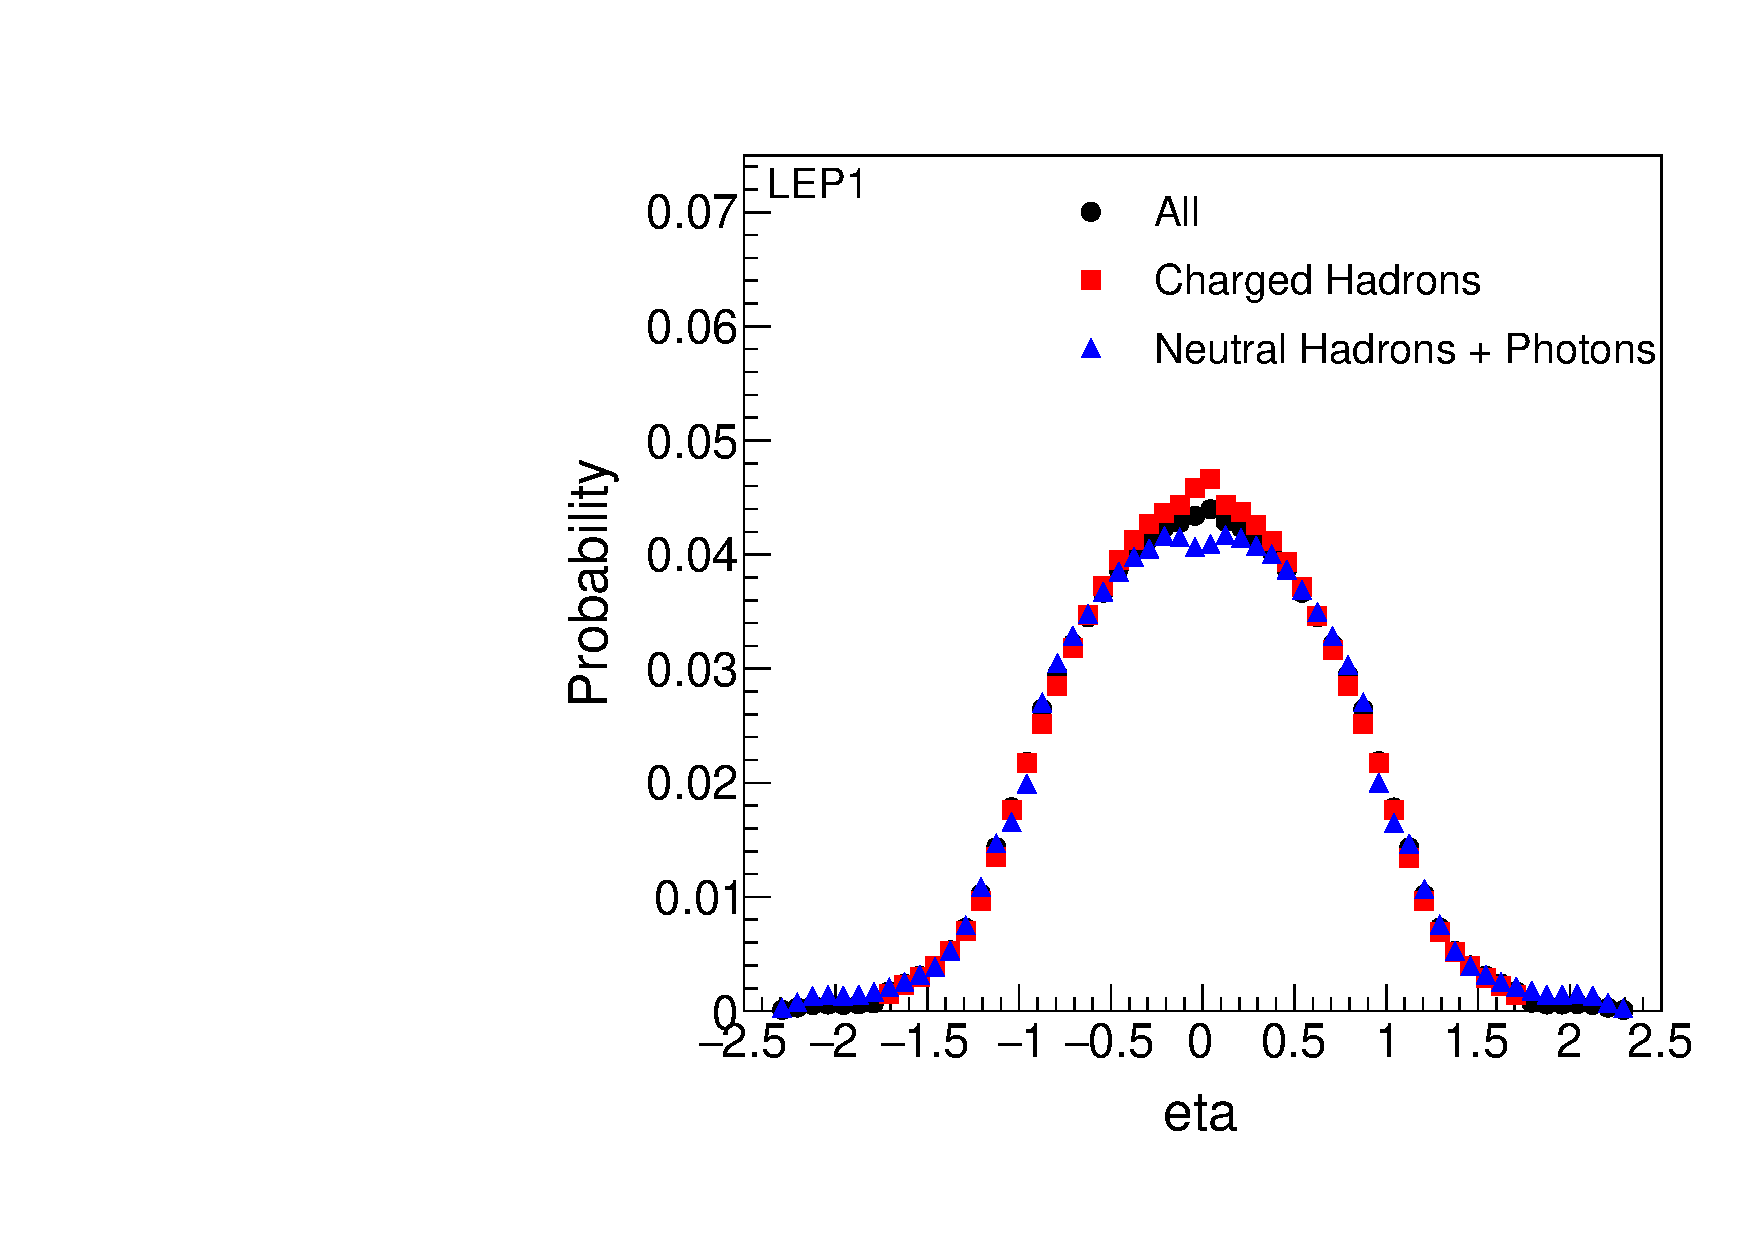
\includegraphics[width=.45\textwidth]{images/DataQualityCheck/LEP1_eta.pdf}
\caption{LEP1 Eta Spectra}
\label{fig:figure1} 
\end{center}
\end{figure}

\begin{figure}[!htb]
\begin{center}
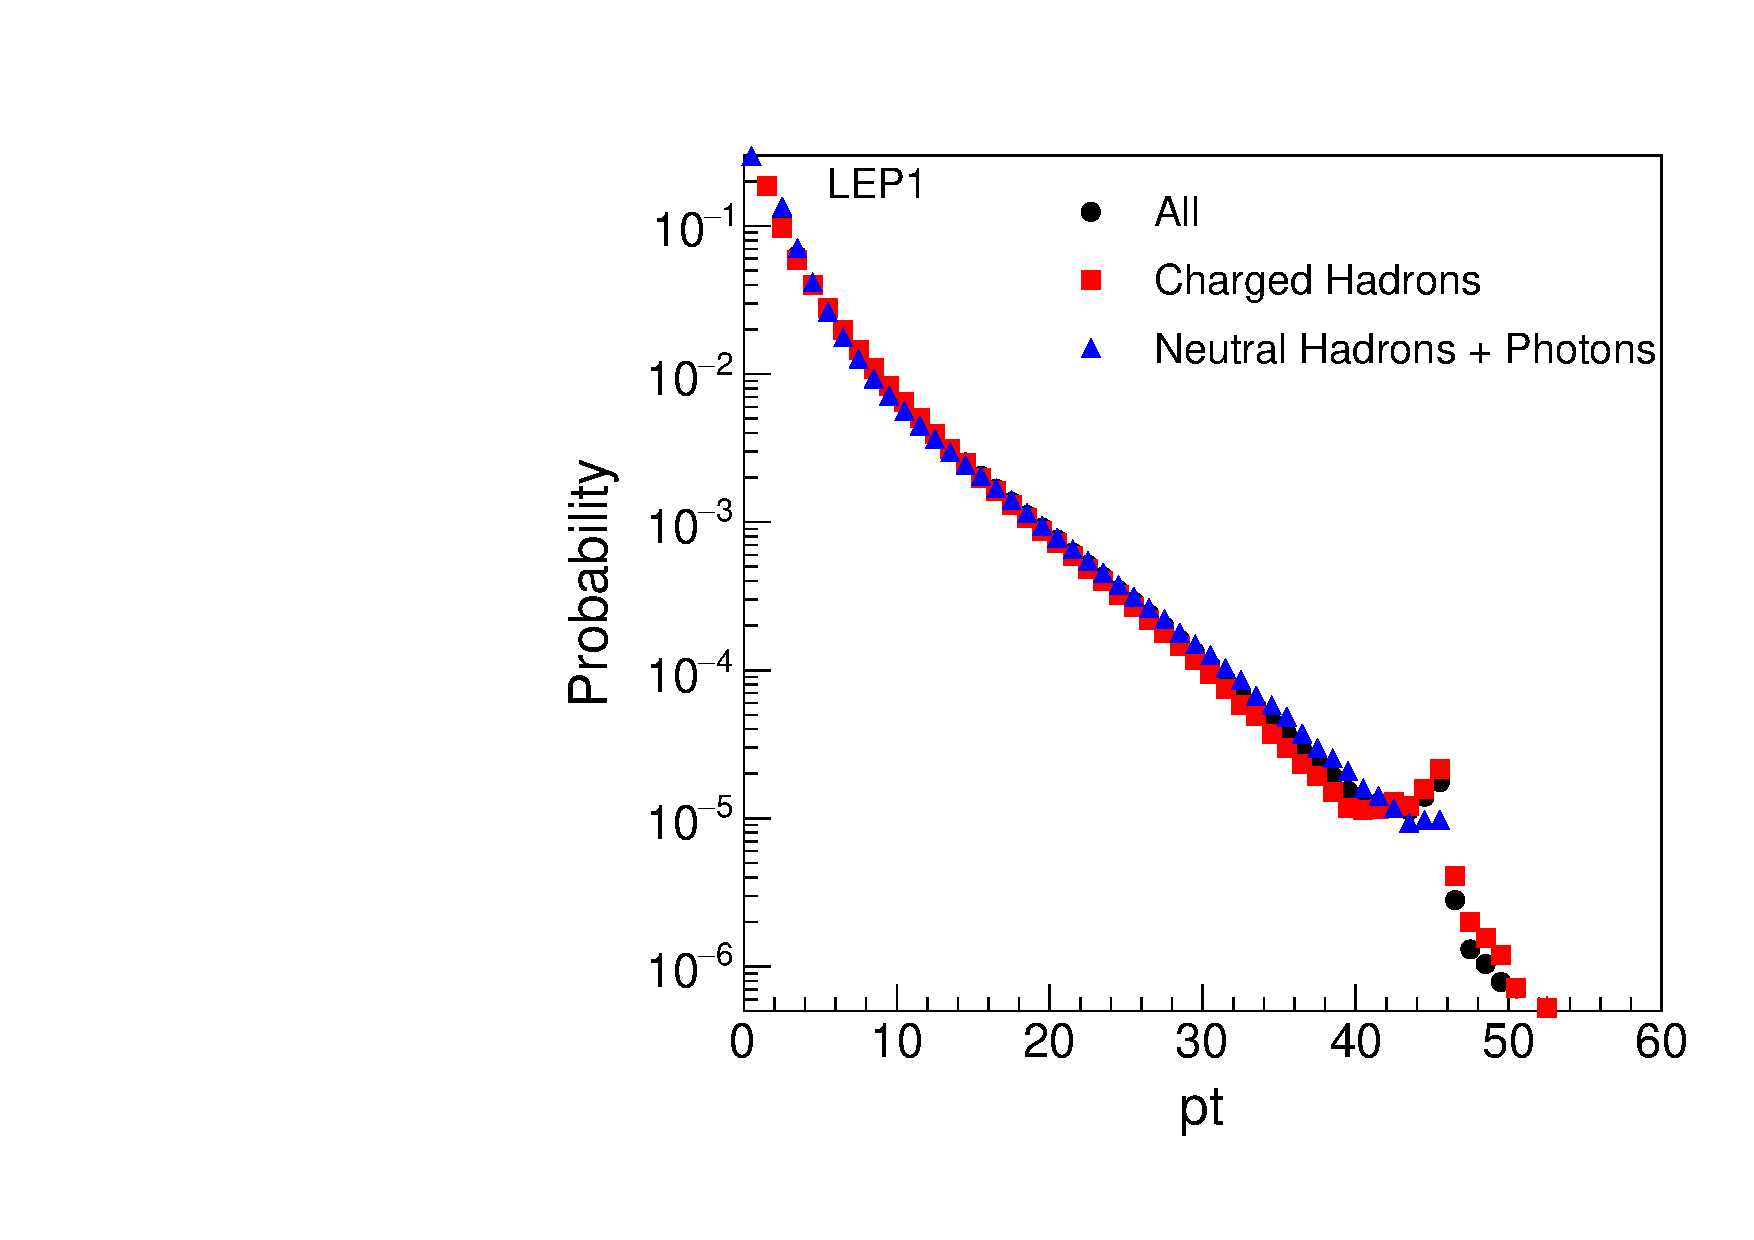
\includegraphics[width=.45\textwidth]{images/DataQualityCheck/LEP1_pt.pdf}
\caption{LEP1 PT spectra}
\label{fig:figure2} 
\end{center}
\end{figure}

\begin{figure}[!htb]
\begin{center}
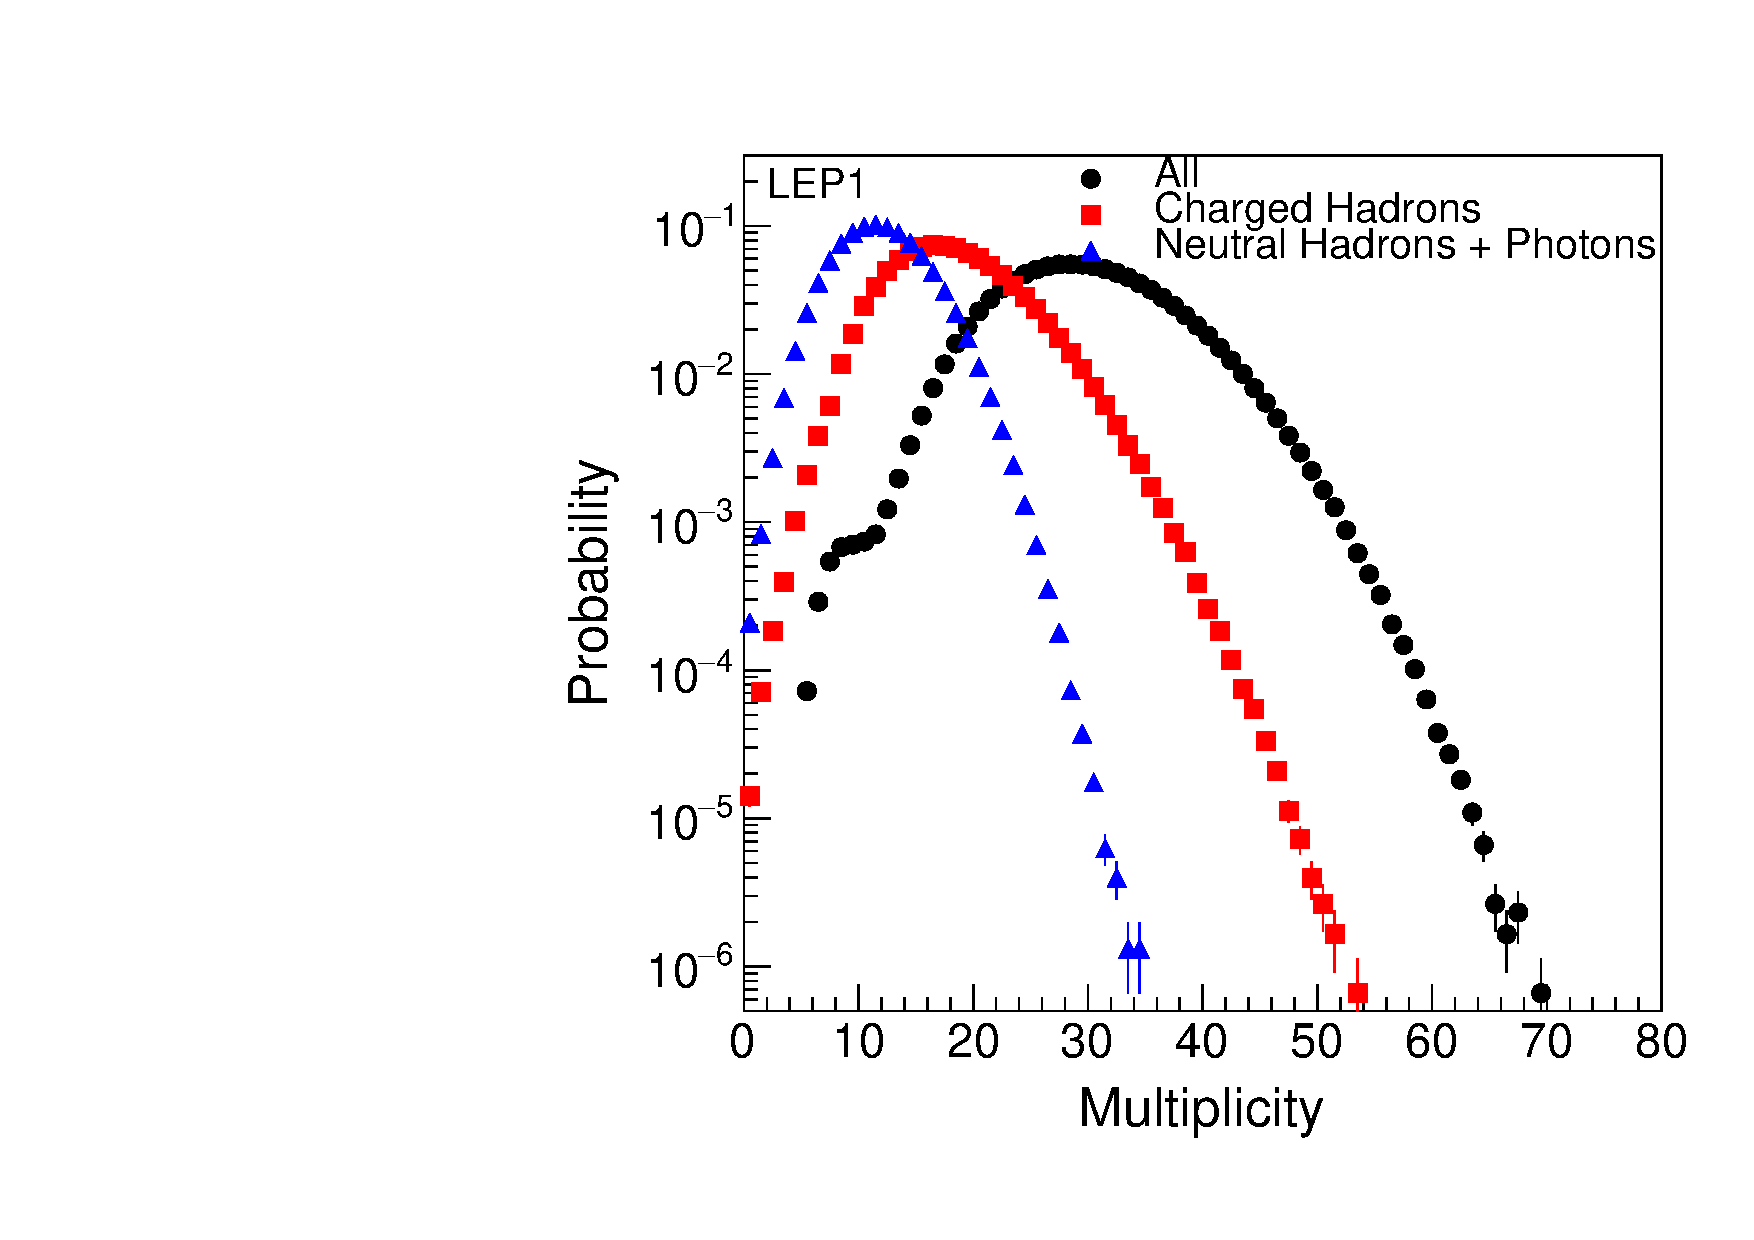
\includegraphics[width=.45\textwidth]{images/DataQualityCheck/LEP1_mult.pdf}
\caption{LEP1 Multiplicity Distribution}
\label{fig:figure6} 
\end{center}
\end{figure}

\begin{figure}[!htb]
\begin{center}
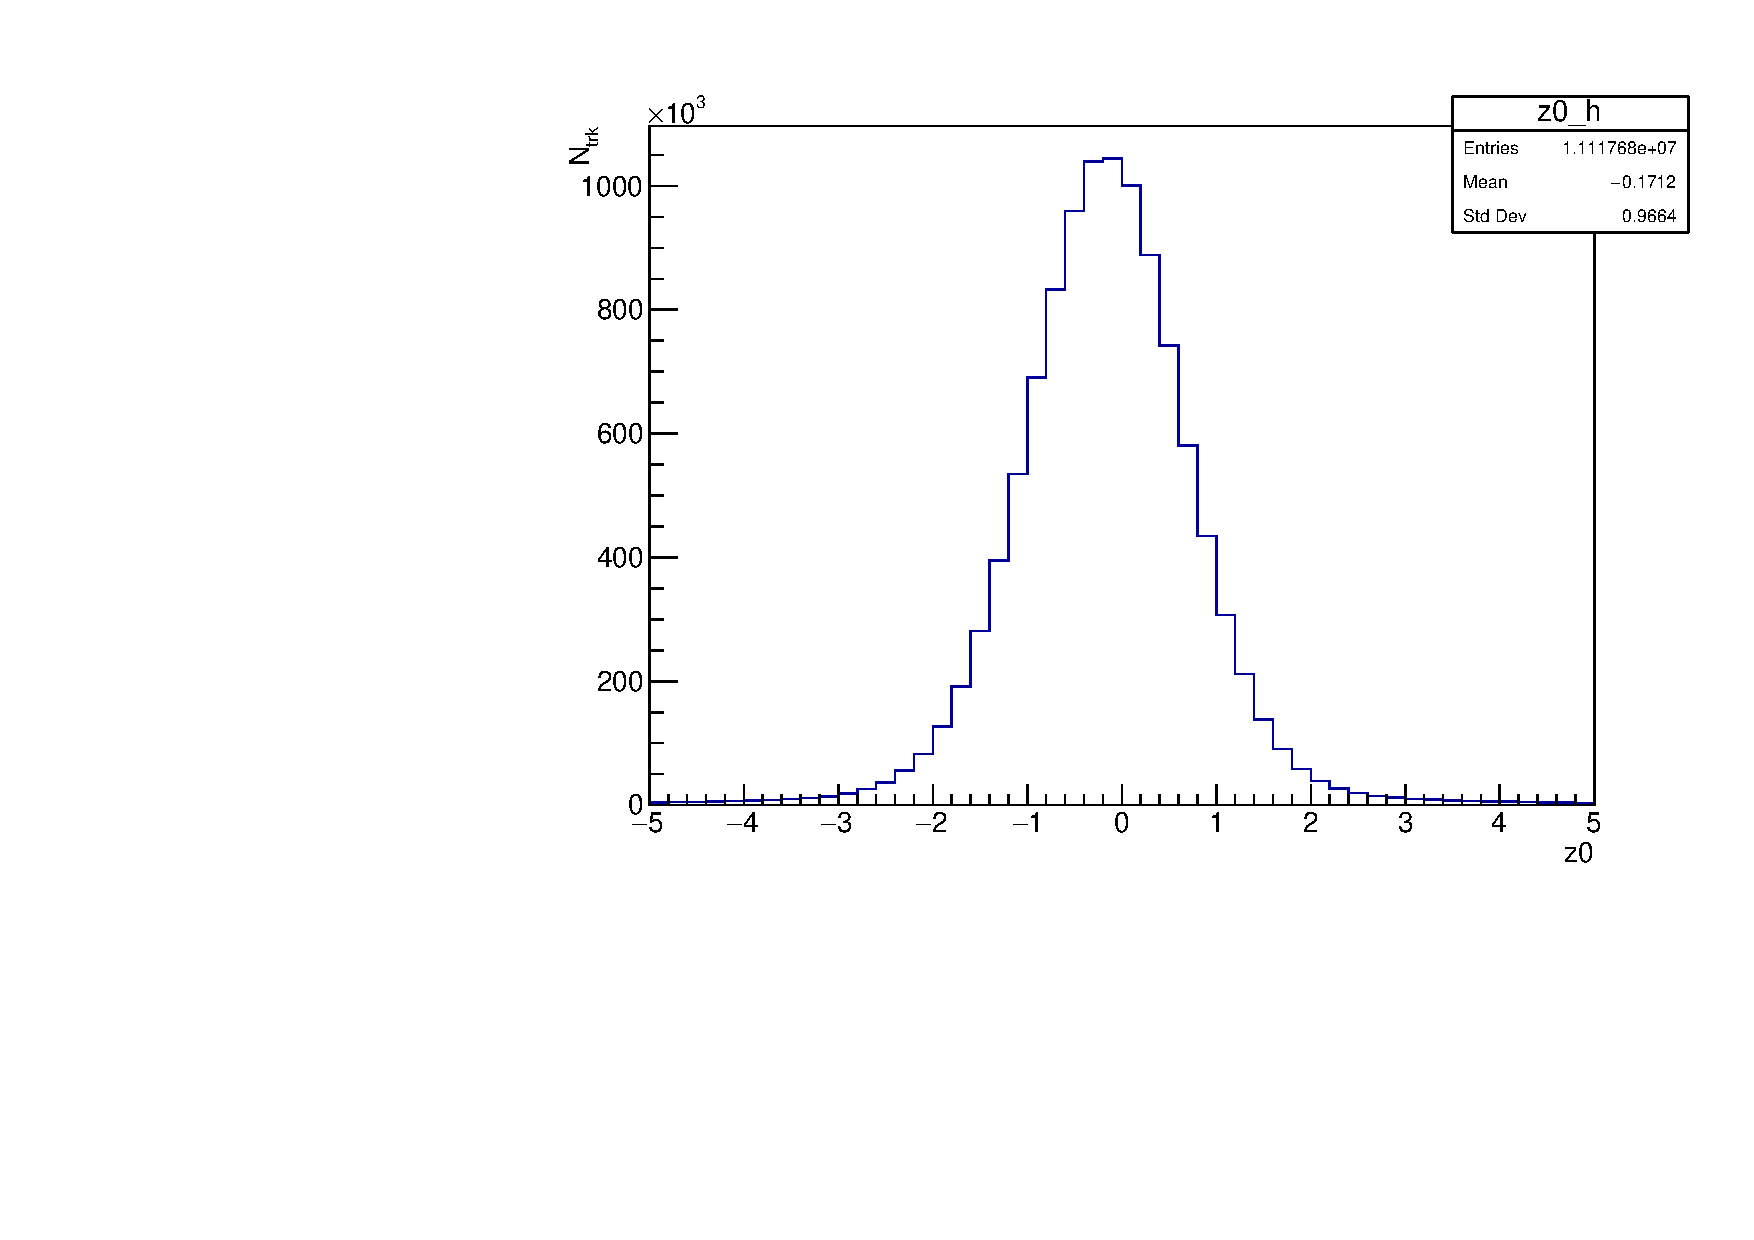
\includegraphics[width=.45\textwidth]{images/DataQualityCheck/z0.pdf}
\caption{LEP1 z distance-of-closest-approach distribution of charged tracks.}
\label{fig:z0} 
\end{center}
\end{figure}

\begin{figure}[!htb]
\begin{center}
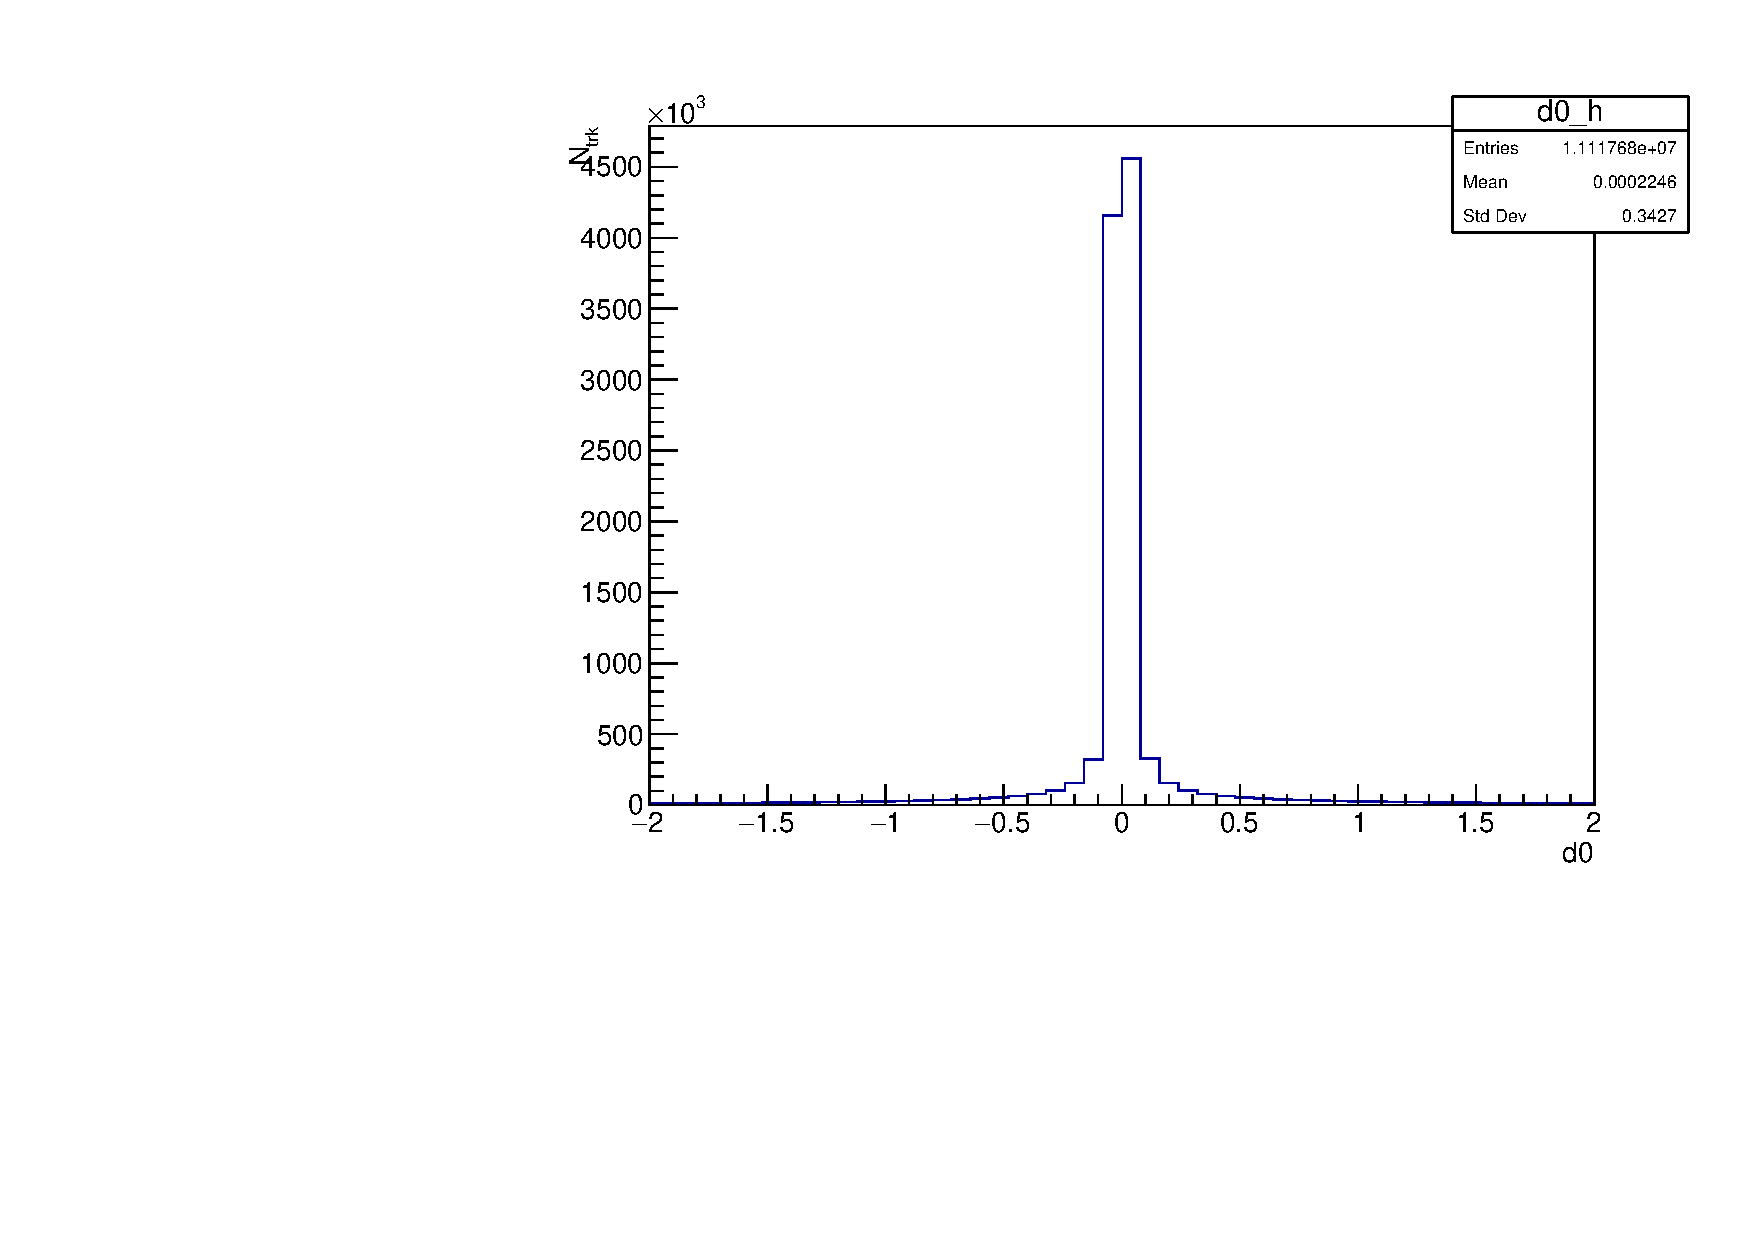
\includegraphics[width=.45\textwidth]{images/DataQualityCheck/d0.pdf}
\caption{LEP1 d0 distribution of charged tracks.}
\label{fig:d0} 
\end{center}
\end{figure}
\begin{figure}[!htb]

\begin{center}
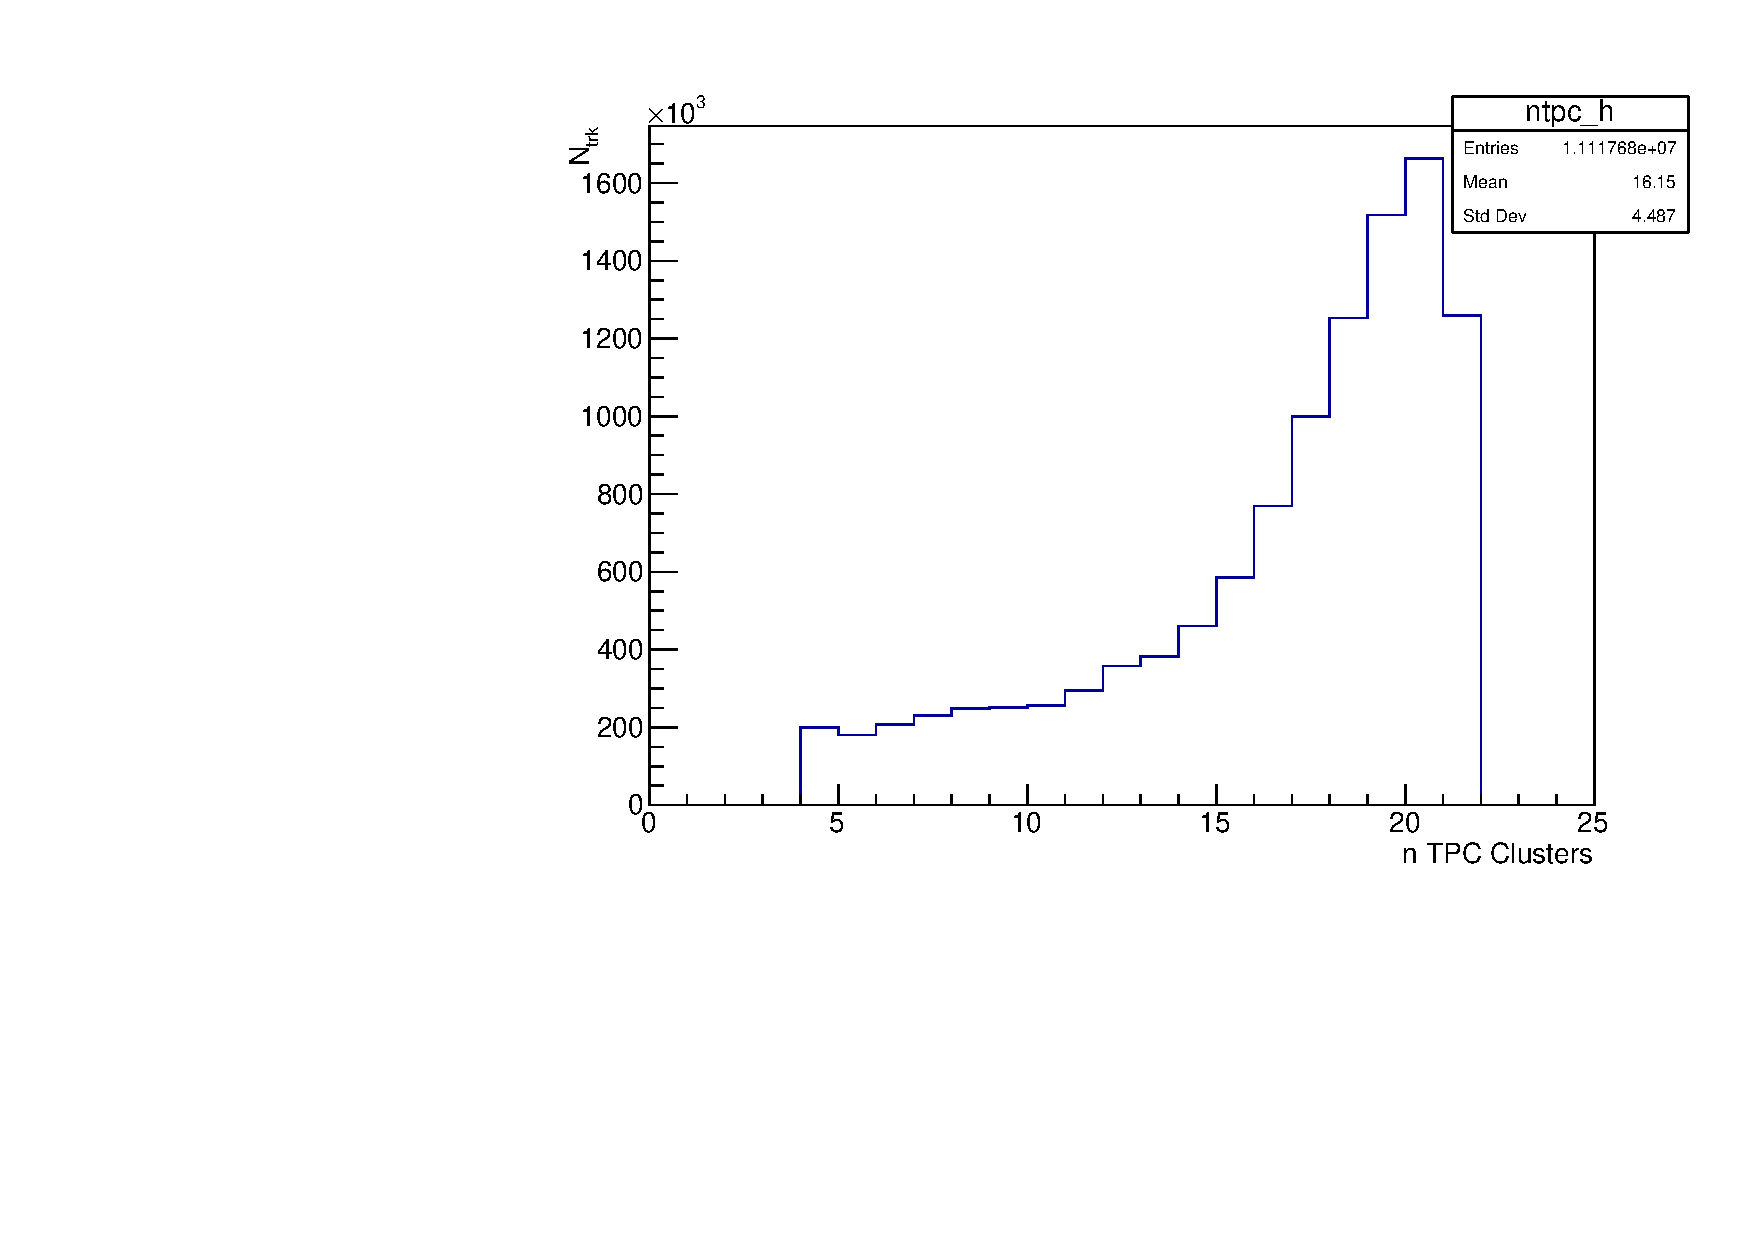
\includegraphics[width=.45\textwidth]{images/DataQualityCheck/ntpc.pdf}
\caption{LEP1 distribution of number of TPC clusters on charged tracks.}
\label{fig:ntpc} 
\end{center}
\end{figure}
\end{comment}

\begin{figure}[H]
\centering
\subfloat{\label{sfig:a}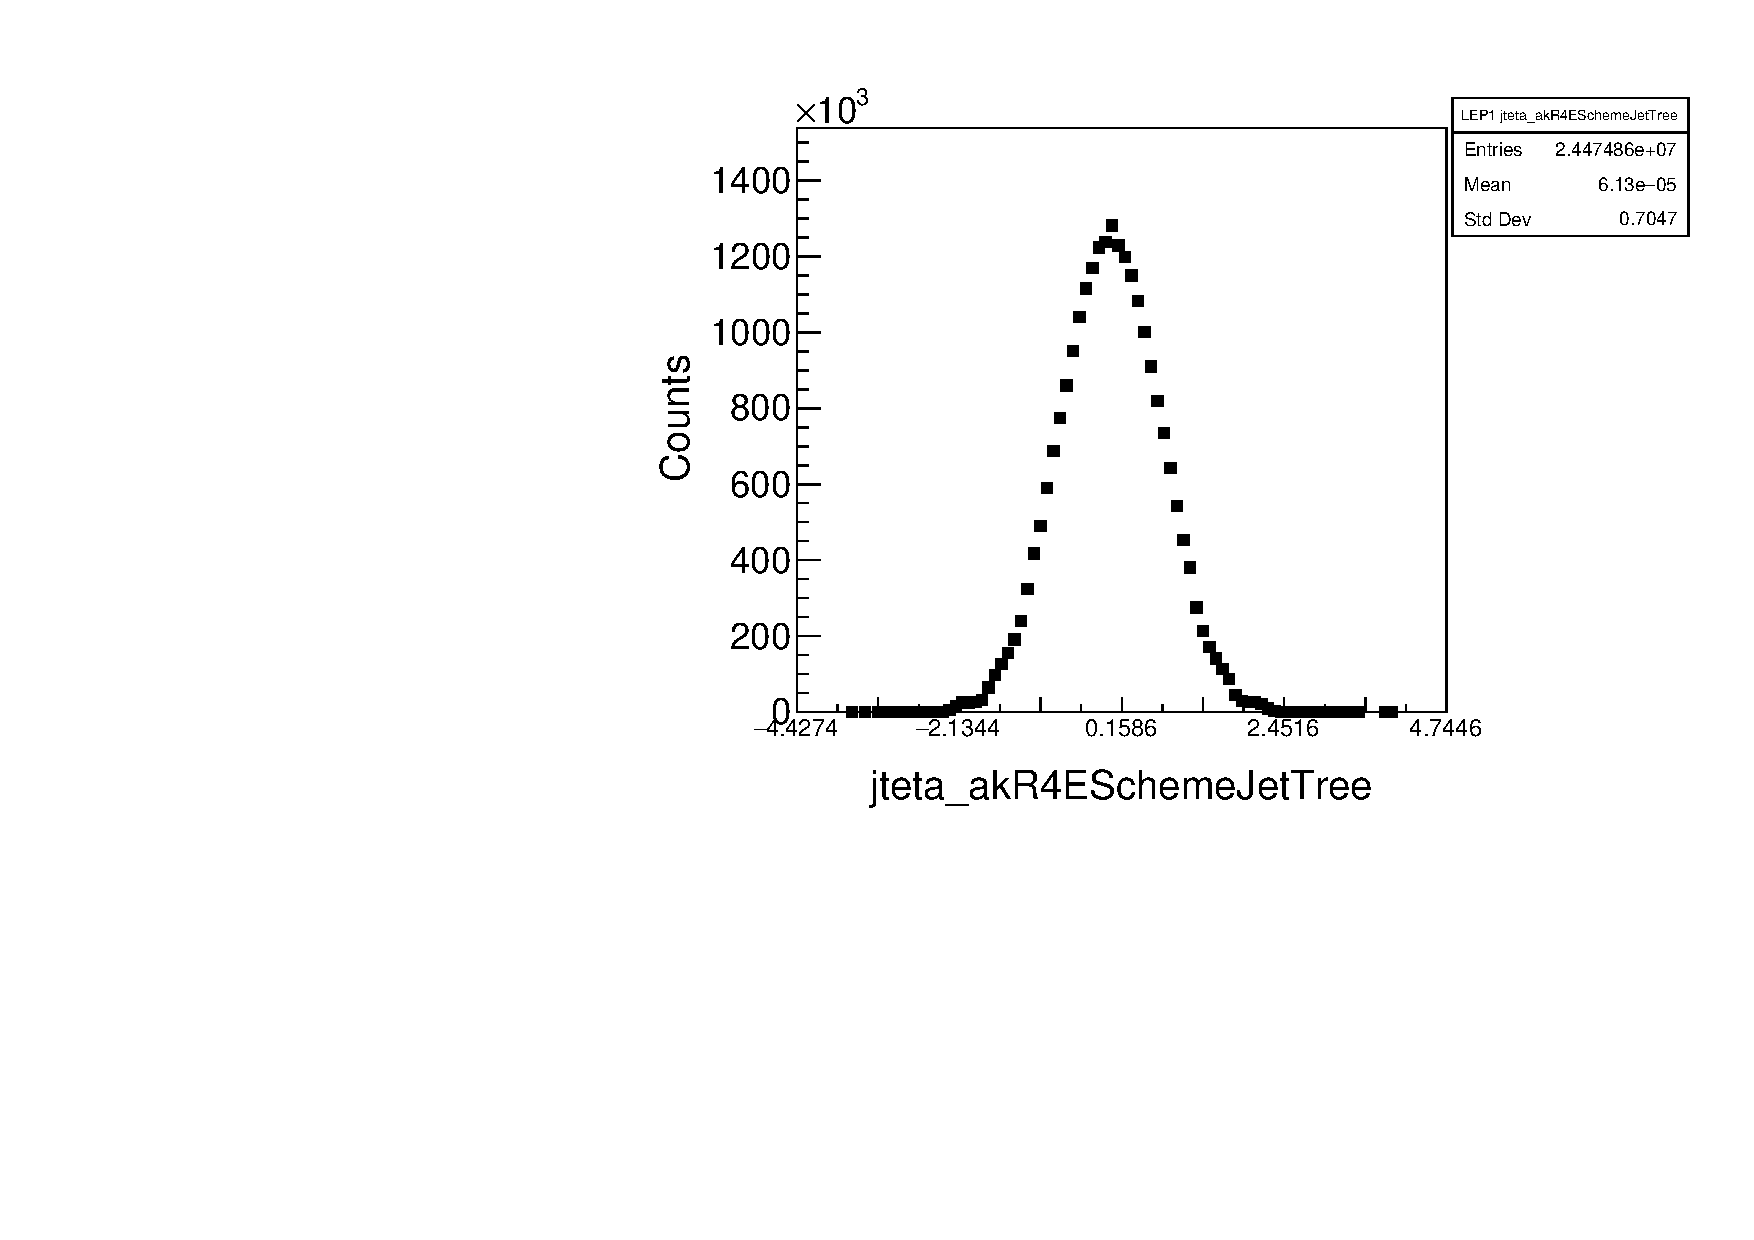
\includegraphics[width=.25\textwidth]{images/DQC/LEP1/jteta_akR4ESchemeJetTree.pdf}}\hfill
\subfloat{\label{sfig:b}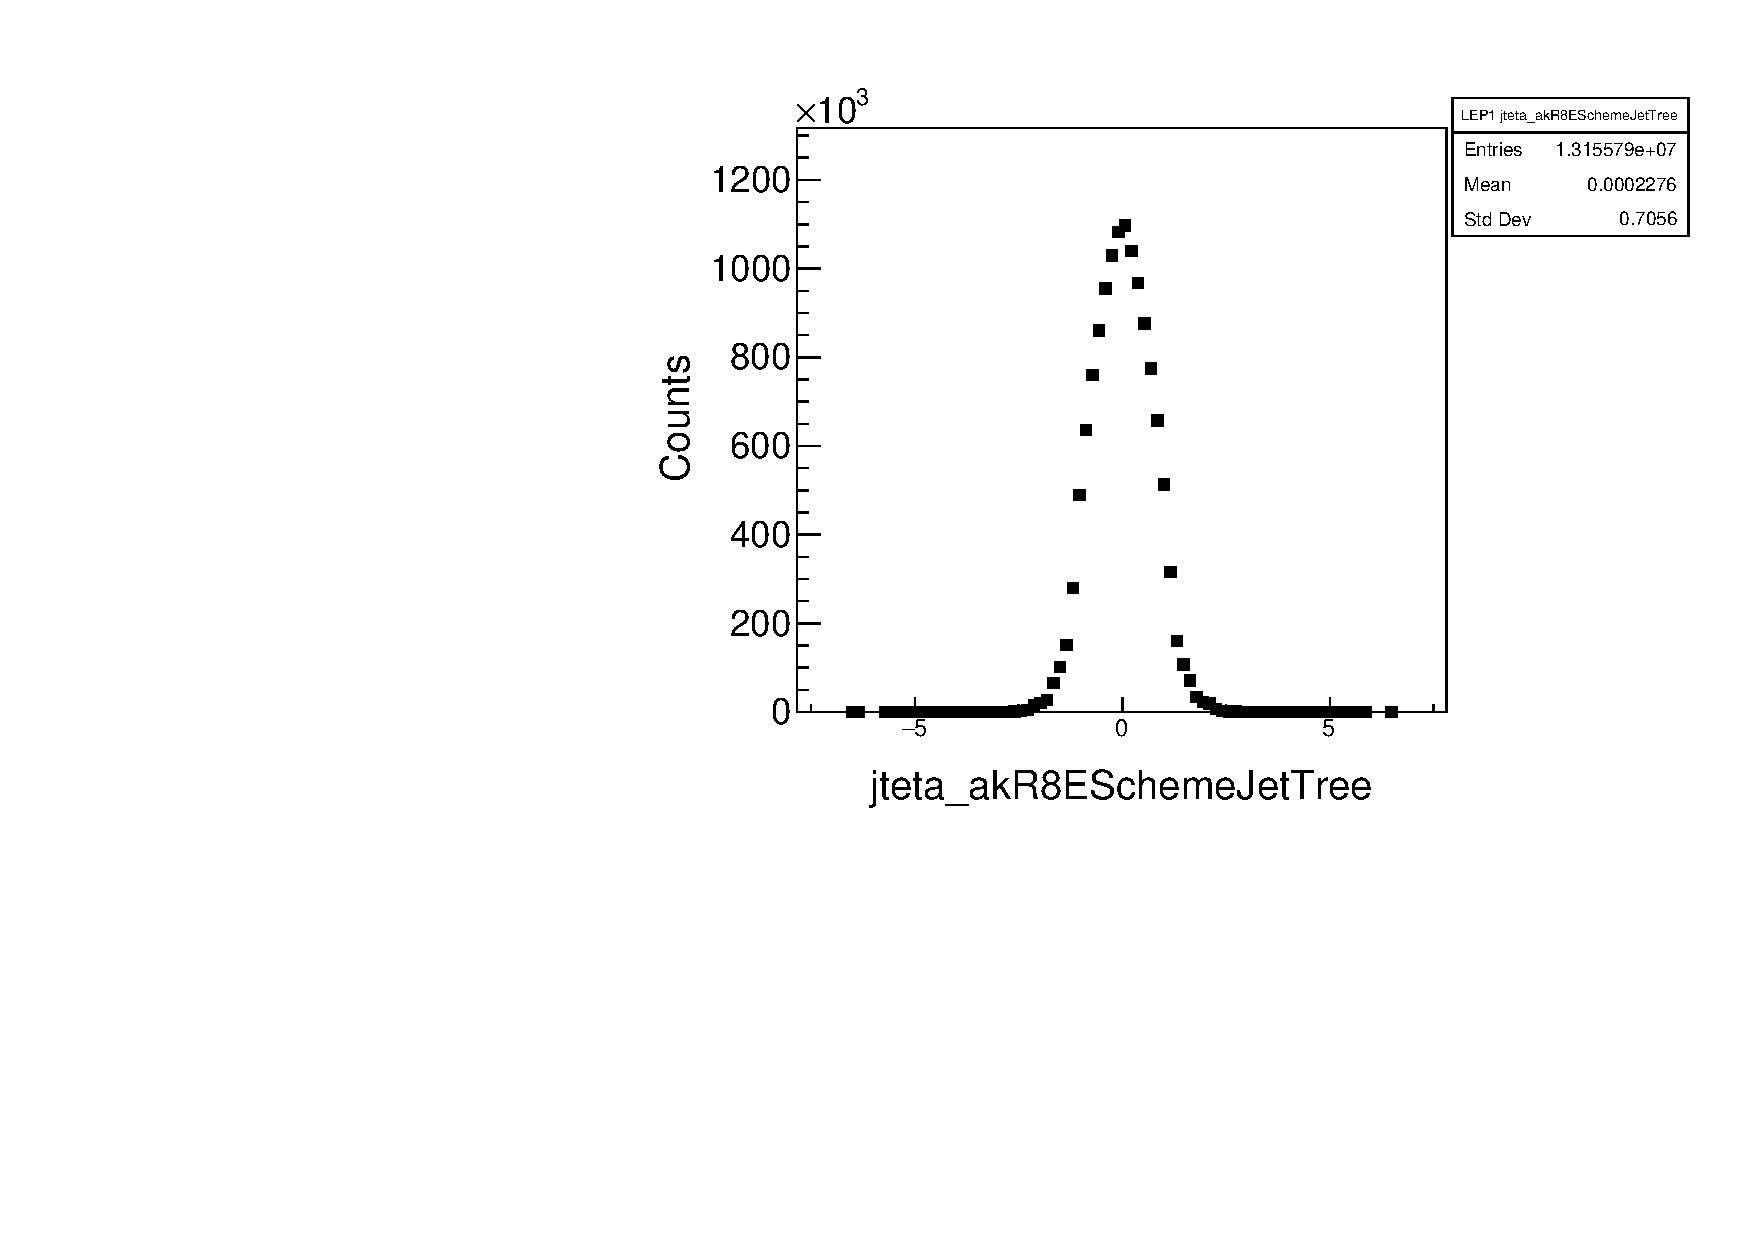
\includegraphics[width=.25\textwidth]{images/DQC/LEP1/jteta_akR8ESchemeJetTree.pdf}}\hfill
\subfloat{\label{sfig:c}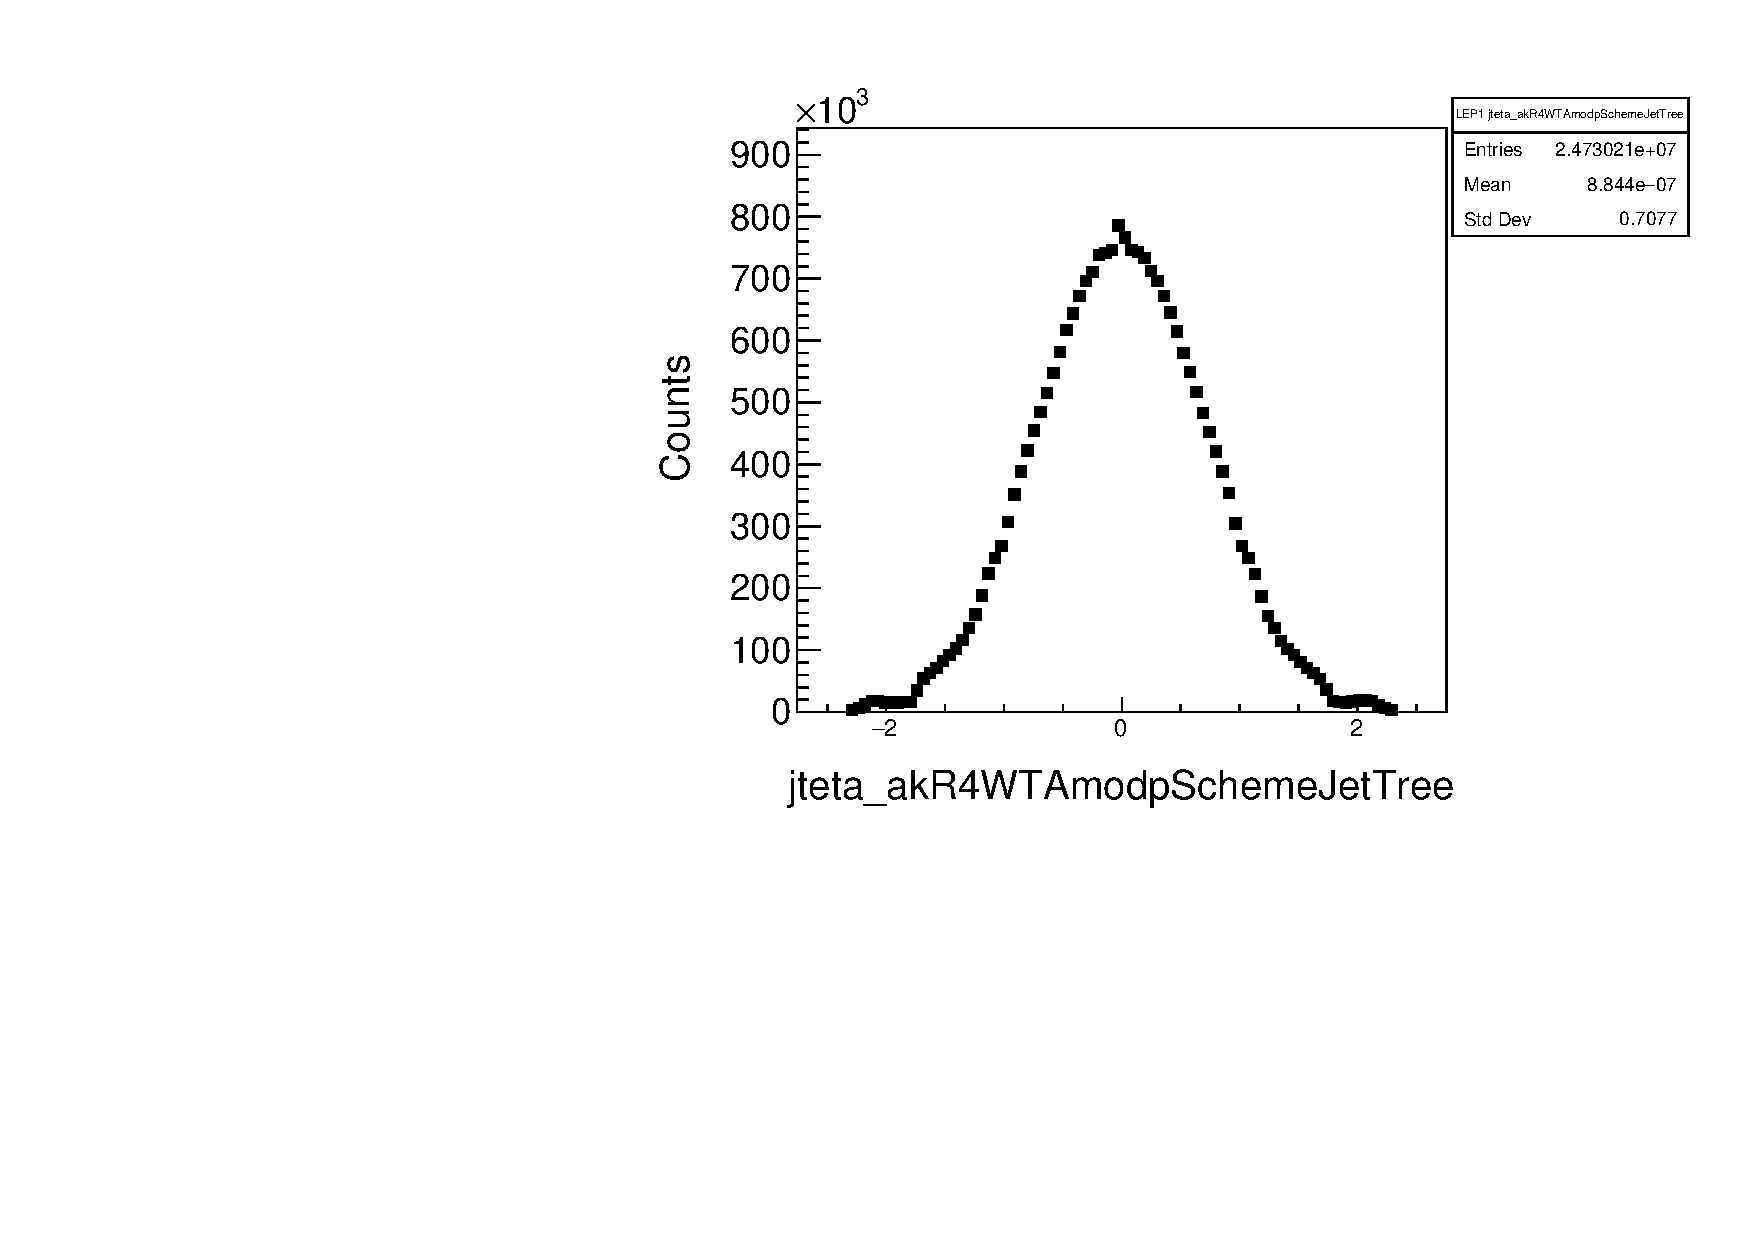
\includegraphics[width=.25\textwidth]{images/DQC/LEP1/jteta_akR4WTAmodpSchemeJetTree.pdf}}\hfill
\subfloat{\label{sfig:d}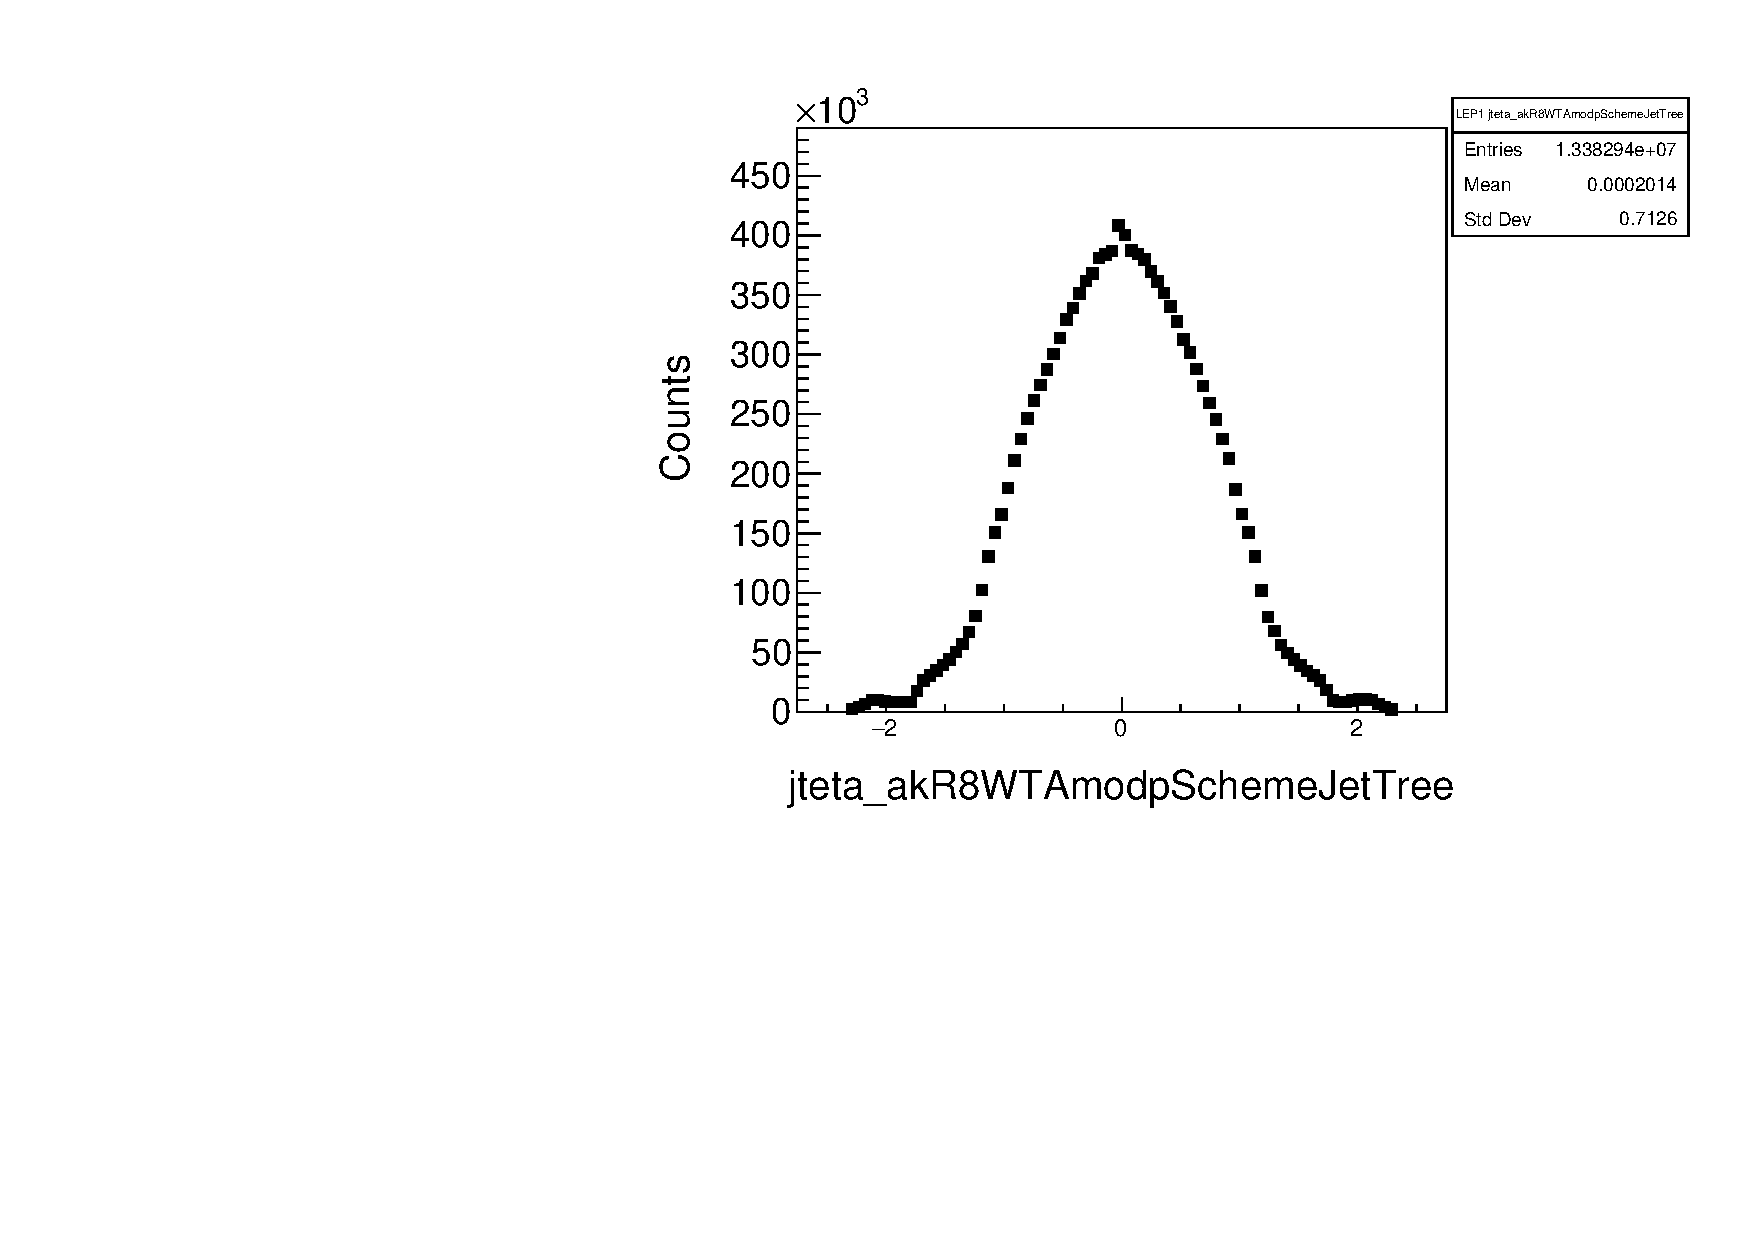
\includegraphics[width=.25\textwidth]{images/DQC/LEP1/jteta_akR8WTAmodpSchemeJetTree.pdf}}\hfill %row end
\subfloat{\label{sfig:e}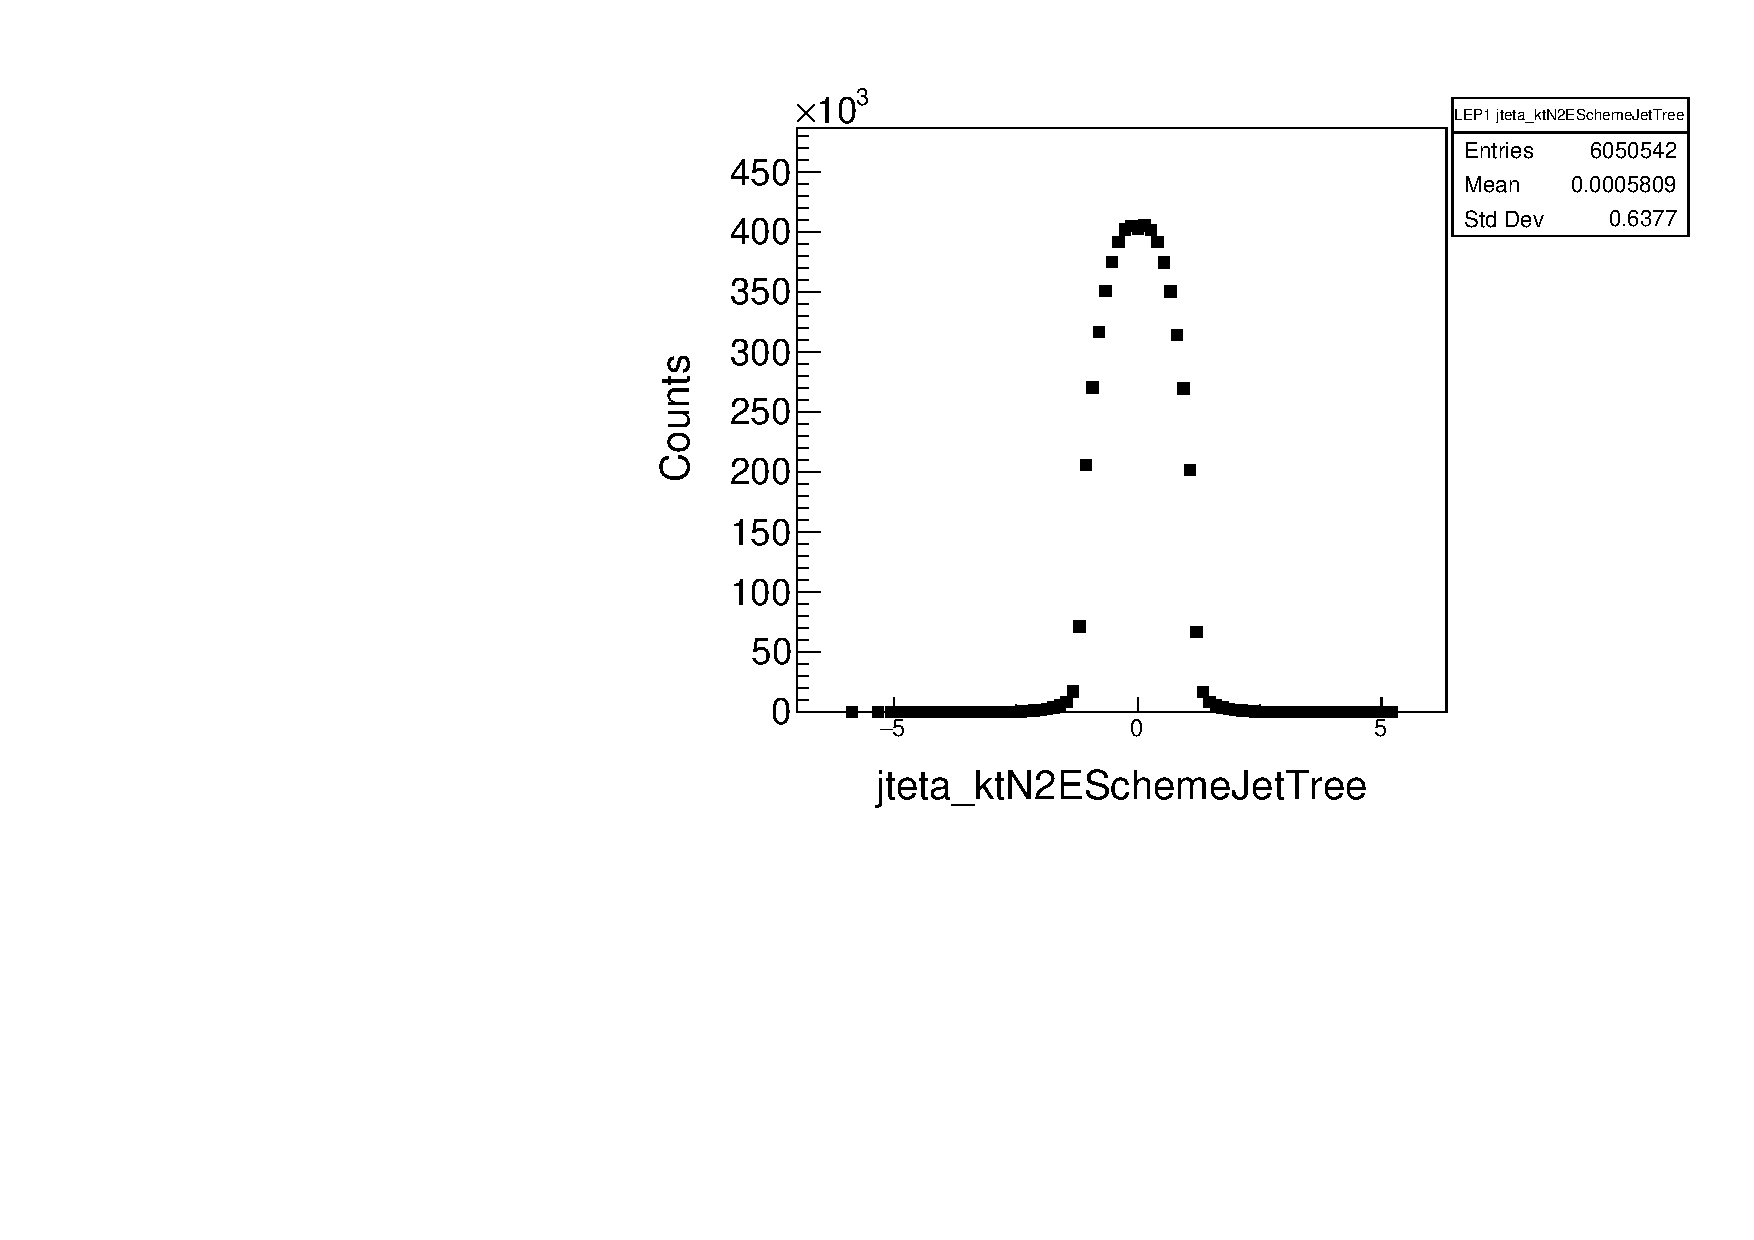
\includegraphics[width=.25\textwidth]{images/DQC/LEP1/jteta_ktN2ESchemeJetTree.pdf}}\hfill
\subfloat{\label{sfig:f}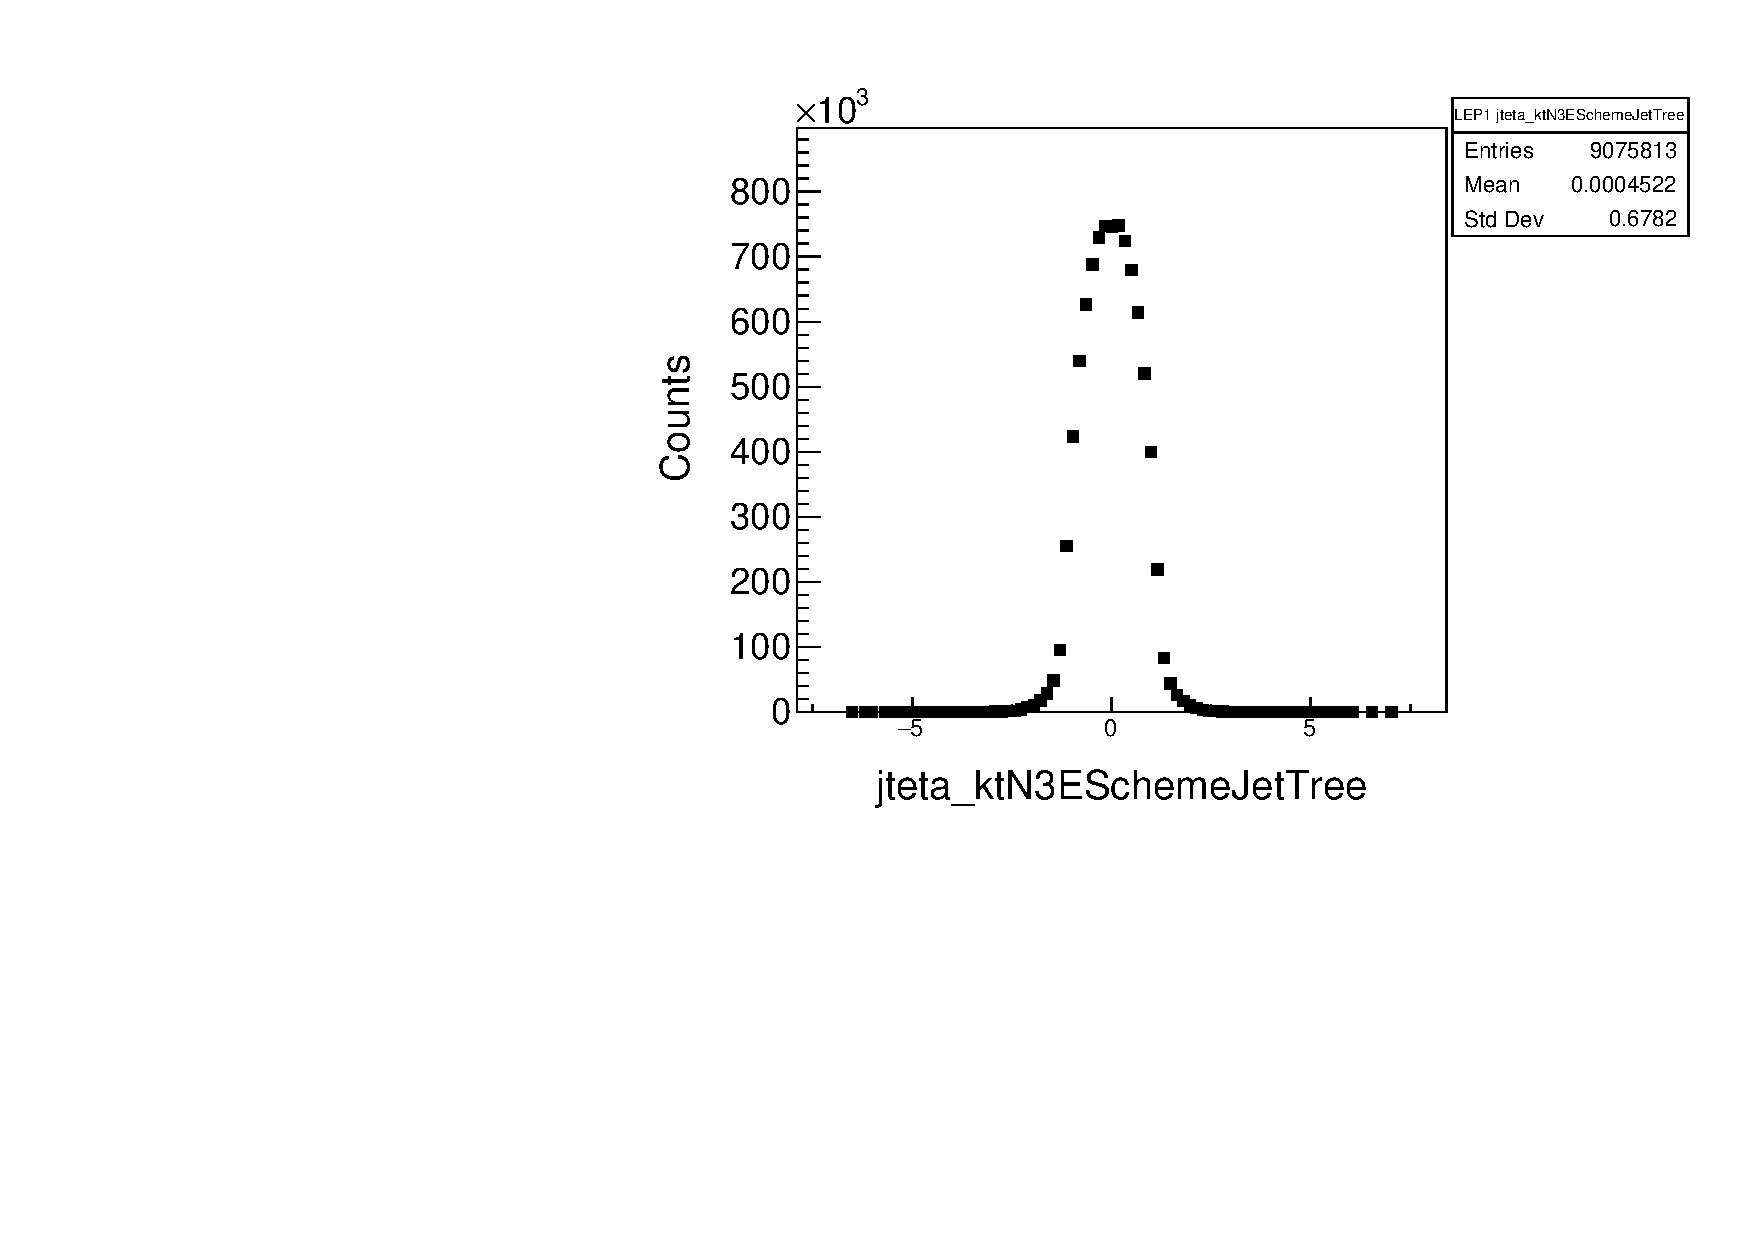
\includegraphics[width=.25\textwidth]{images/DQC/LEP1/jteta_ktN3ESchemeJetTree.pdf}}\hfill
\subfloat{\label{sfig:g}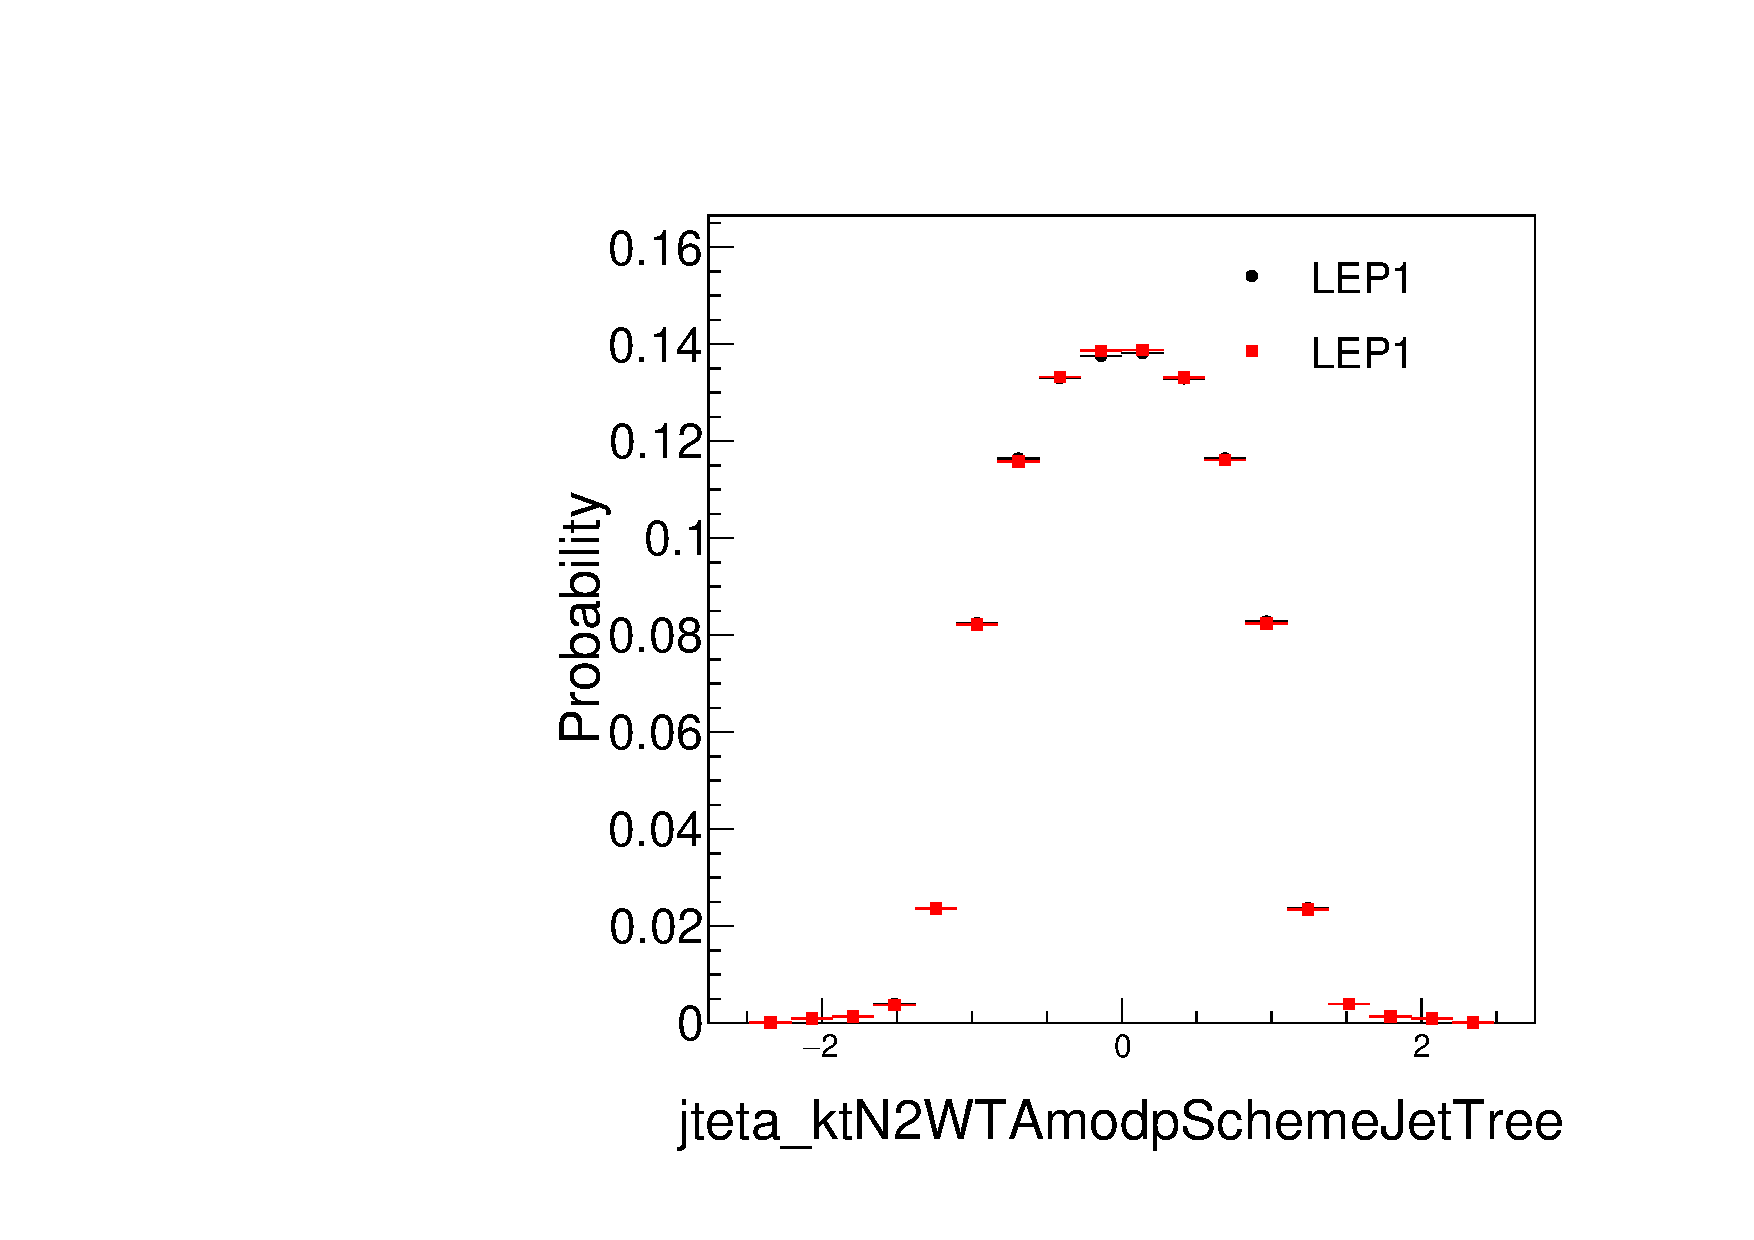
\includegraphics[width=.25\textwidth]{images/DQC/LEP1/jteta_ktN2WTAmodpSchemeJetTree.pdf}}\hfill
\subfloat{\label{sfig:h}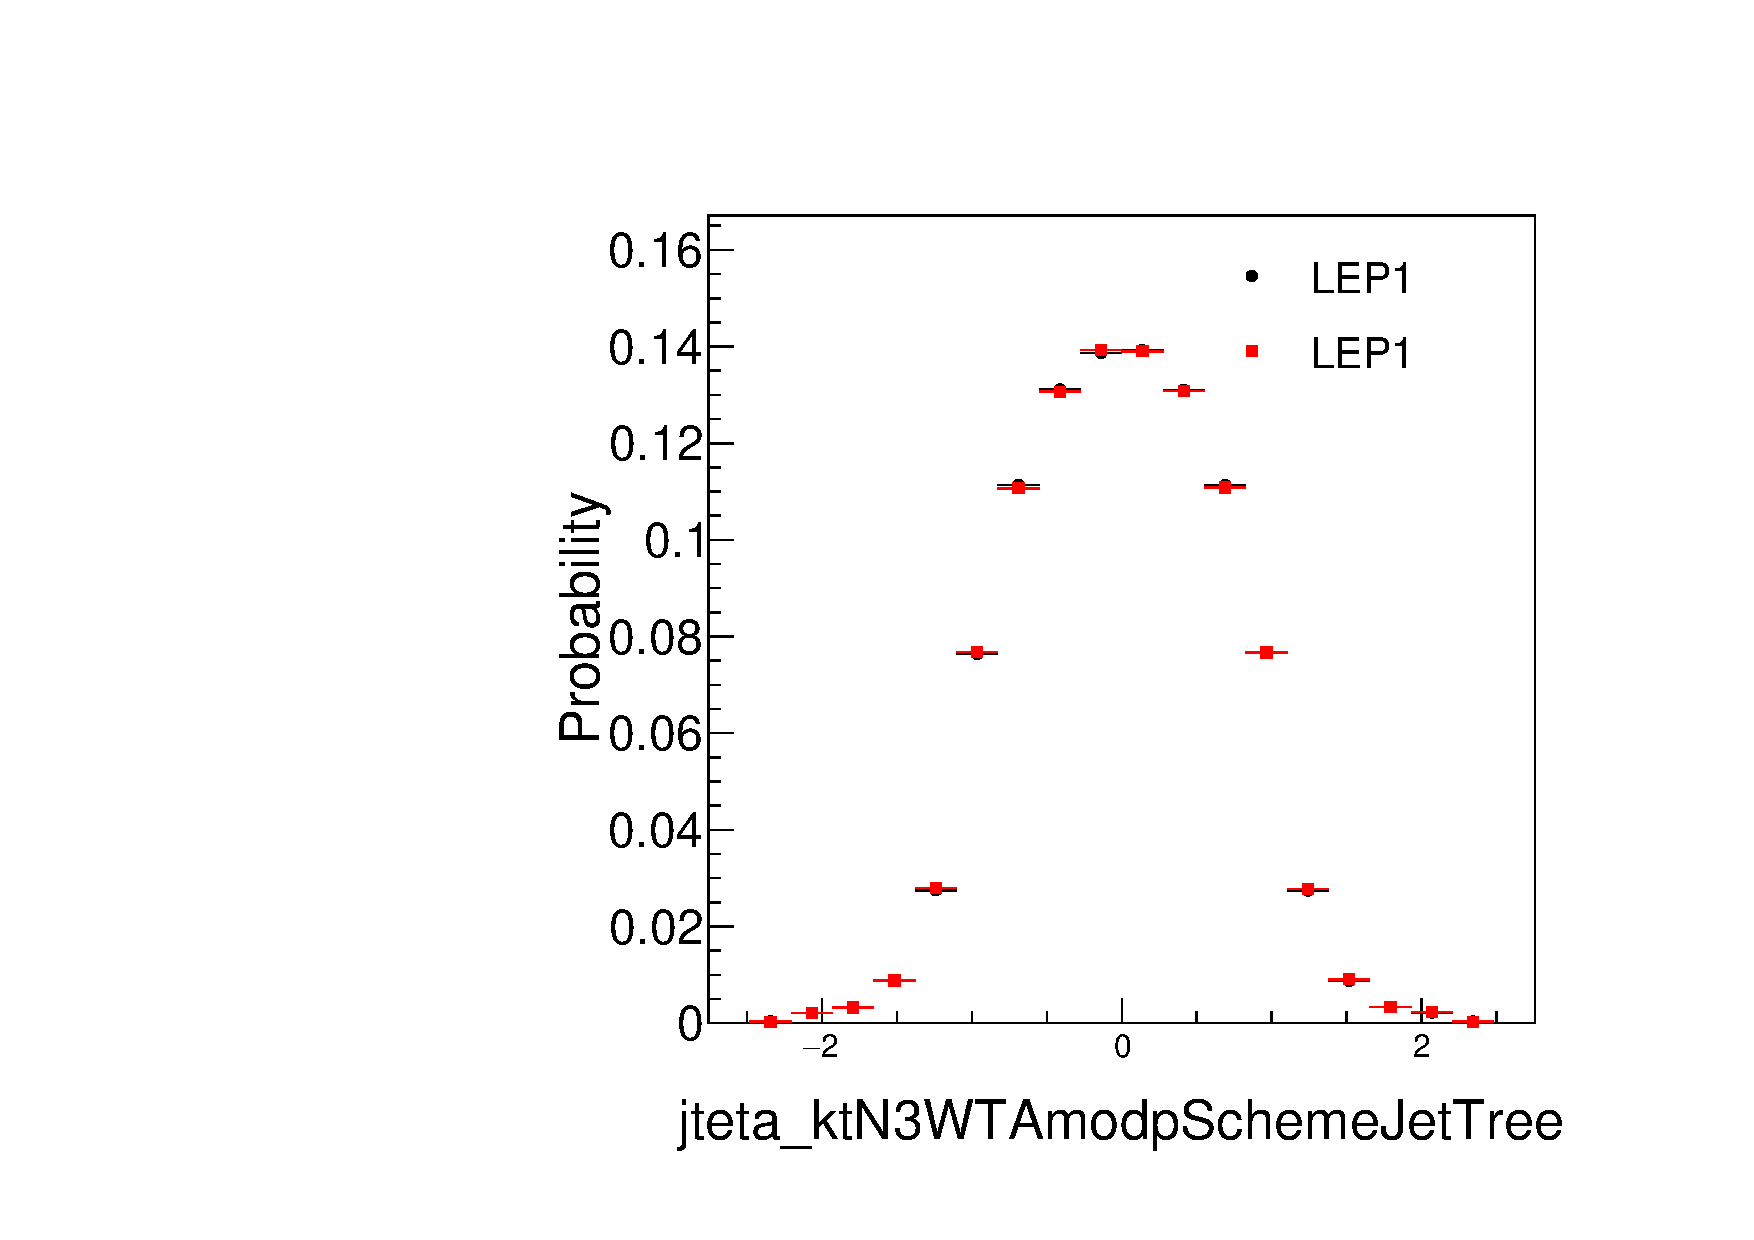
\includegraphics[width=.25\textwidth]{images/DQC/LEP1/jteta_ktN3WTAmodpSchemeJetTree.pdf}}\hfill
\caption{LEP1 Jet $\eta$ distributions. Top row: anti-$k_t$, left to right: $R=0.4$, $E$ scheme; $R=0.8$, $E$ scheme; $R=0.4$, WTA mod p scheme; $R=0.8$, WTA mod p scheme. Bottom row: $k_t$, left to right: $N=2$, $E$ scheme; $N=3$, $E$ scheme; $N=2$, WTA mod p scheme; $N=3$; WTA mod p scheme.}  
\end{figure}

\begin{figure}[H]
\centering
\subfloat{\label{sfig:a}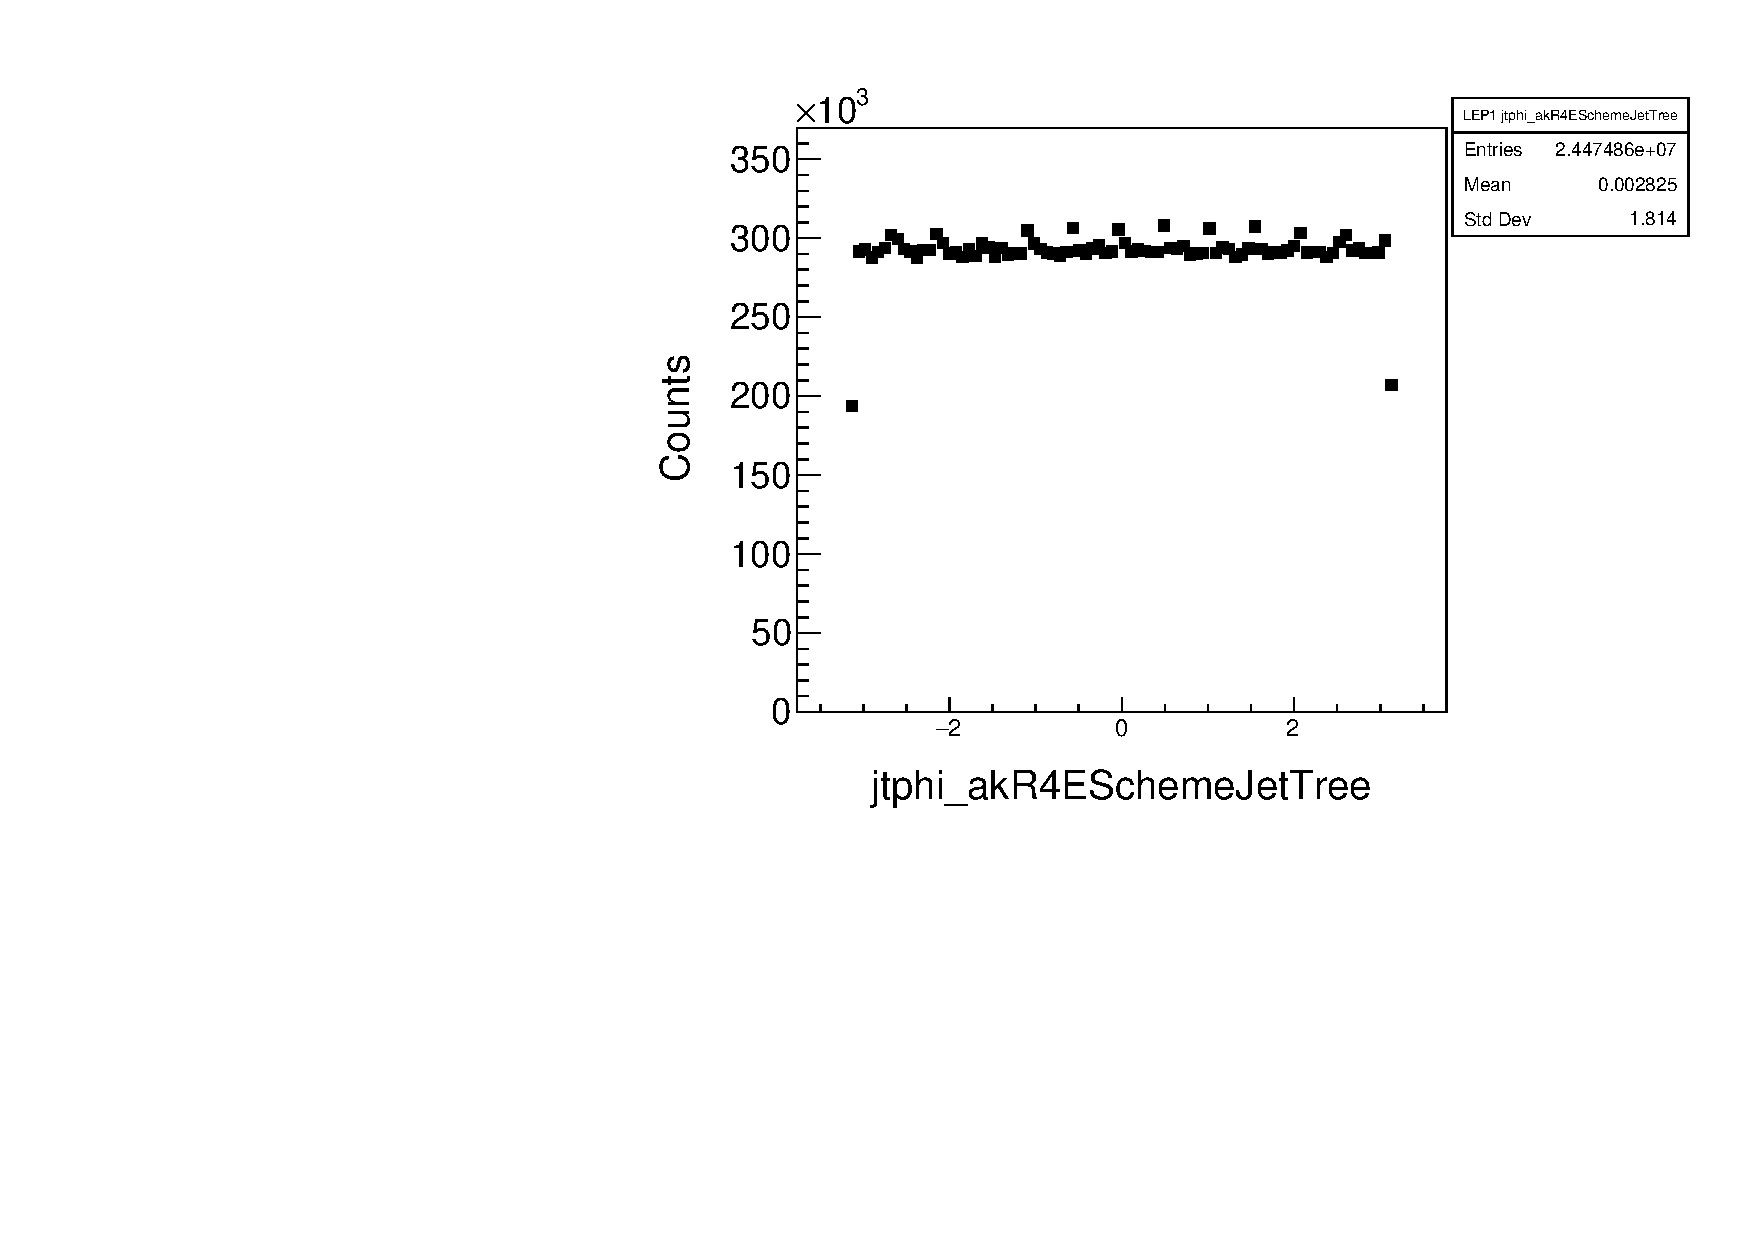
\includegraphics[width=.25\textwidth]{images/DQC/LEP1/jtphi_akR4ESchemeJetTree.pdf}}\hfill
\subfloat{\label{sfig:b}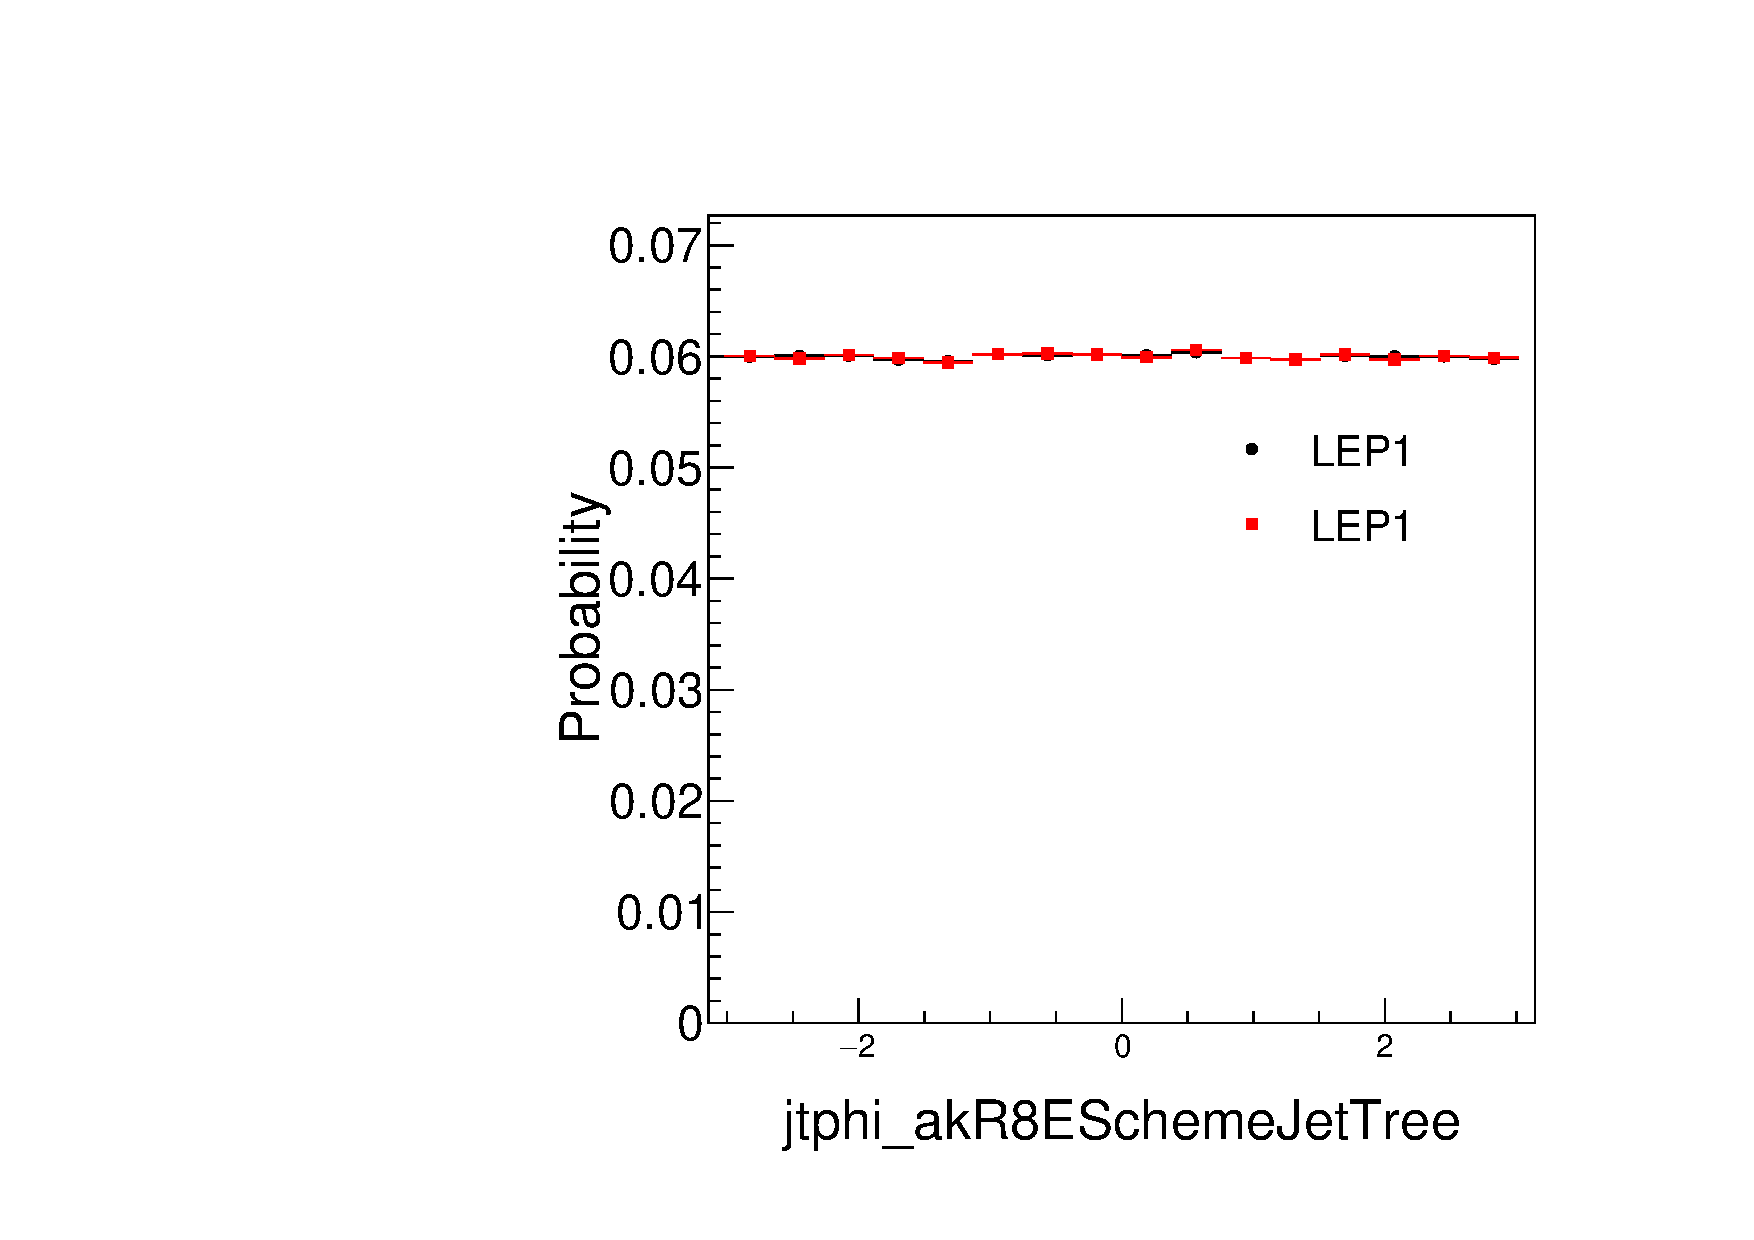
\includegraphics[width=.25\textwidth]{images/DQC/LEP1/jtphi_akR8ESchemeJetTree.pdf}}\hfill
\subfloat{\label{sfig:c}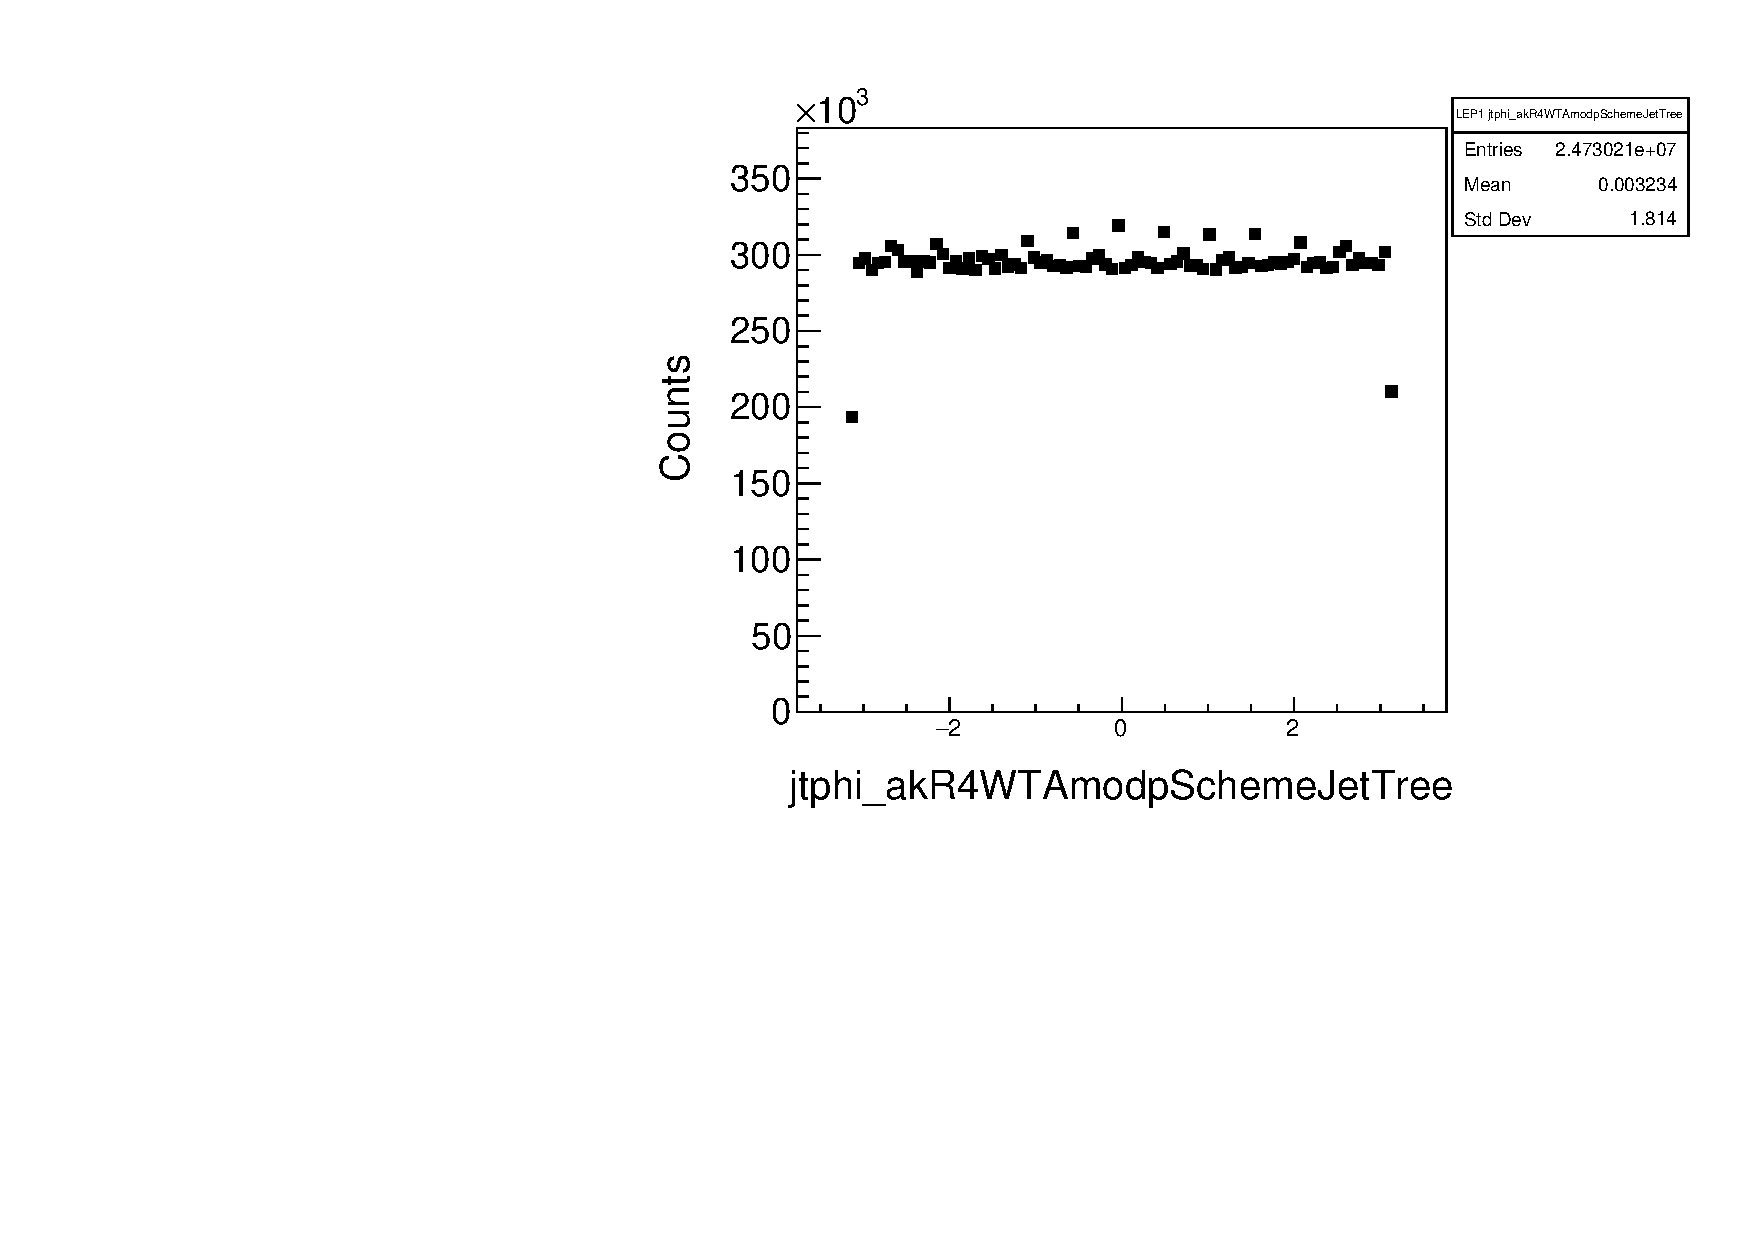
\includegraphics[width=.25\textwidth]{images/DQC/LEP1/jtphi_akR4WTAmodpSchemeJetTree.pdf}}\hfill
\subfloat{\label{sfig:d}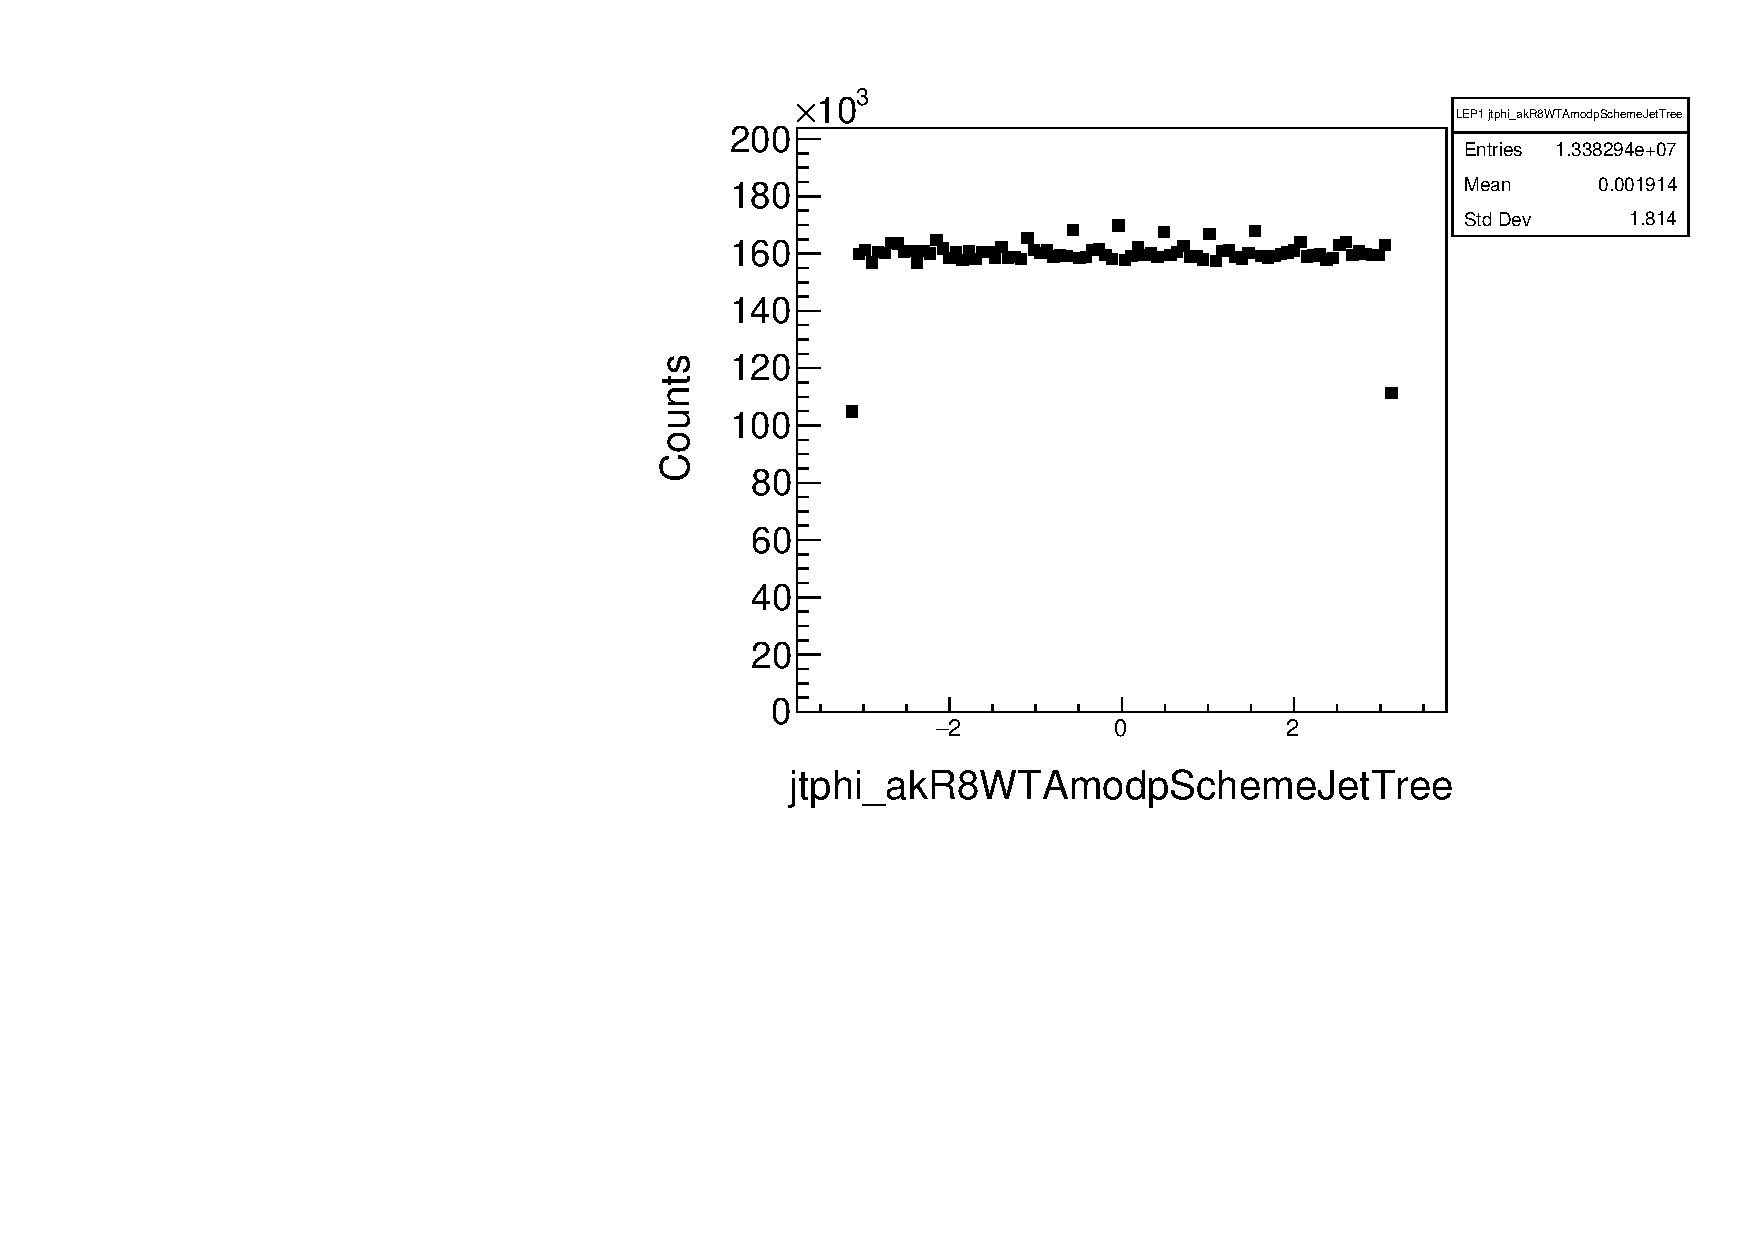
\includegraphics[width=.25\textwidth]{images/DQC/LEP1/jtphi_akR8WTAmodpSchemeJetTree.pdf}}\hfill %row end
\subfloat{\label{sfig:e}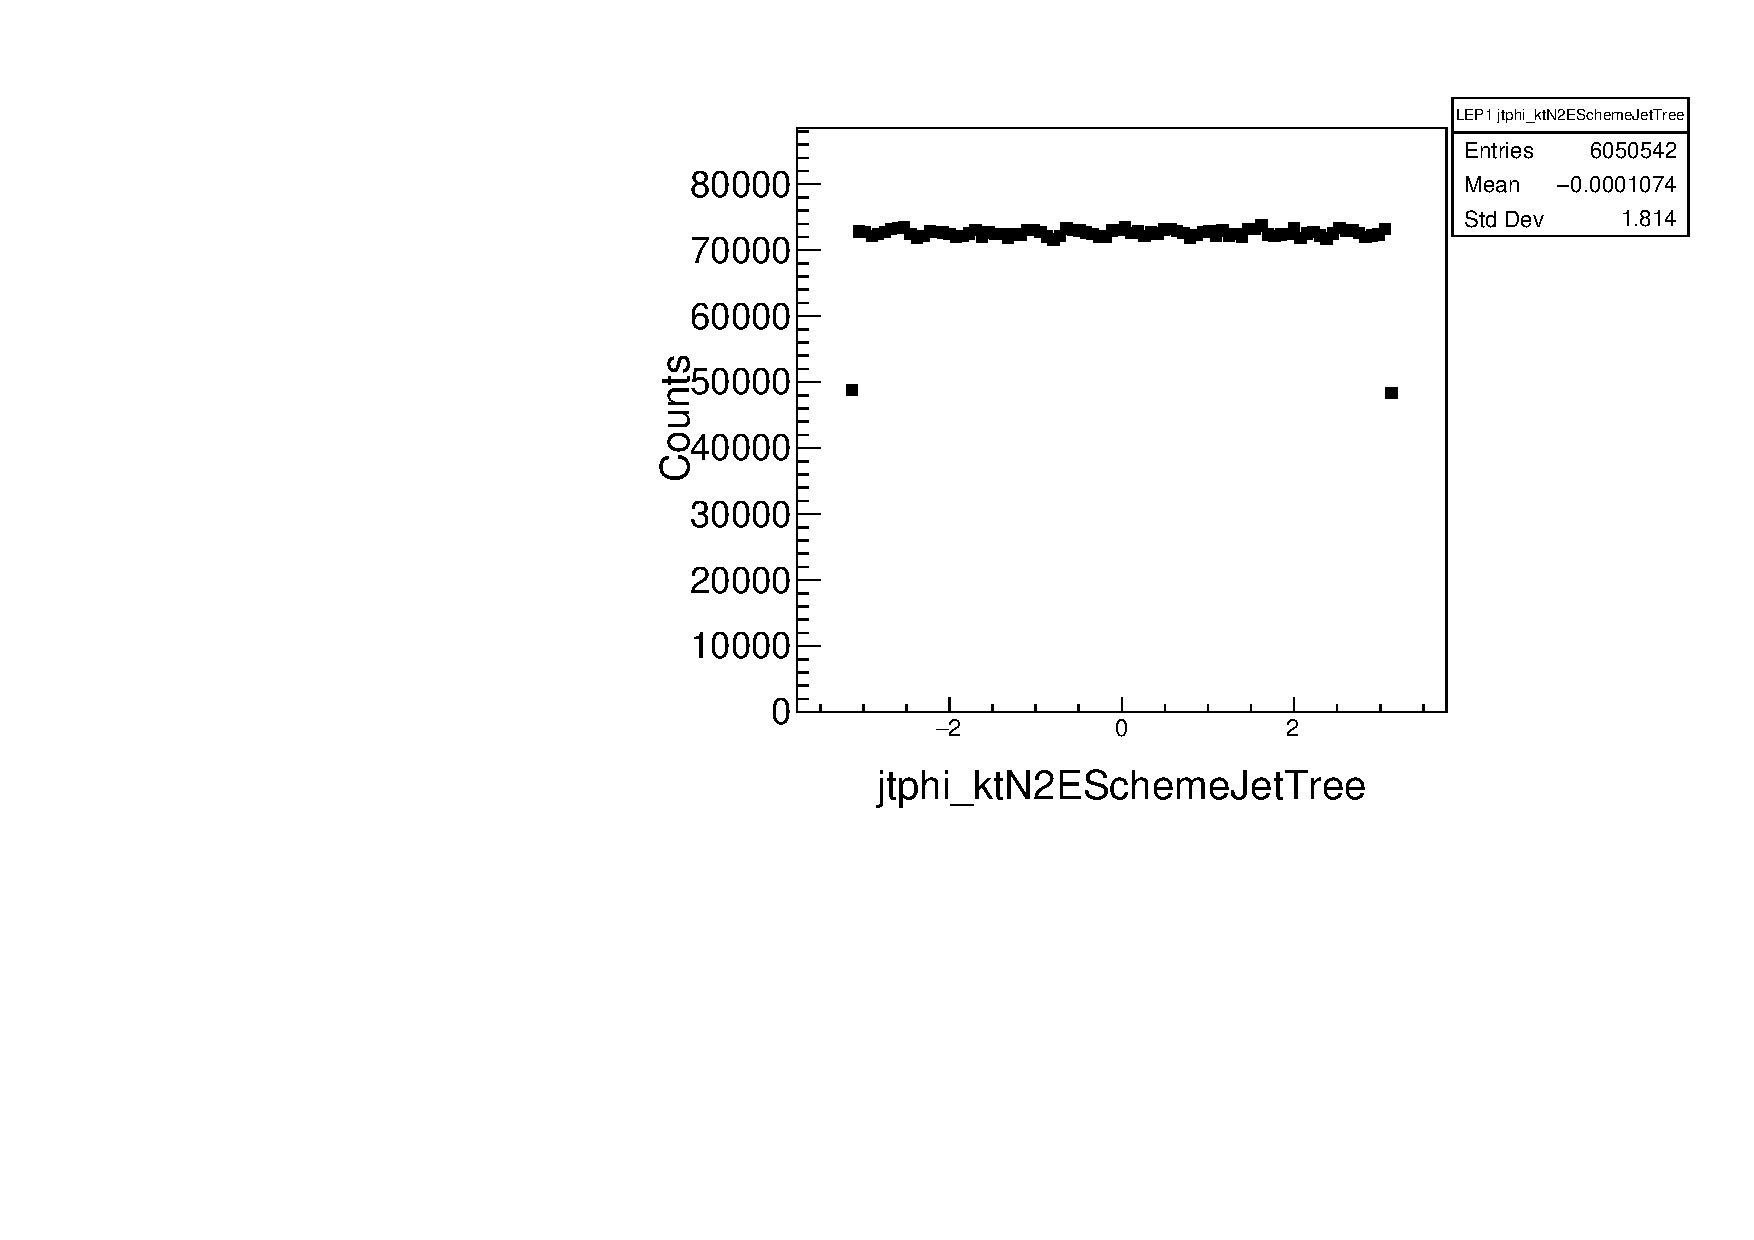
\includegraphics[width=.25\textwidth]{images/DQC/LEP1/jtphi_ktN2ESchemeJetTree.pdf}}\hfill
\subfloat{\label{sfig:f}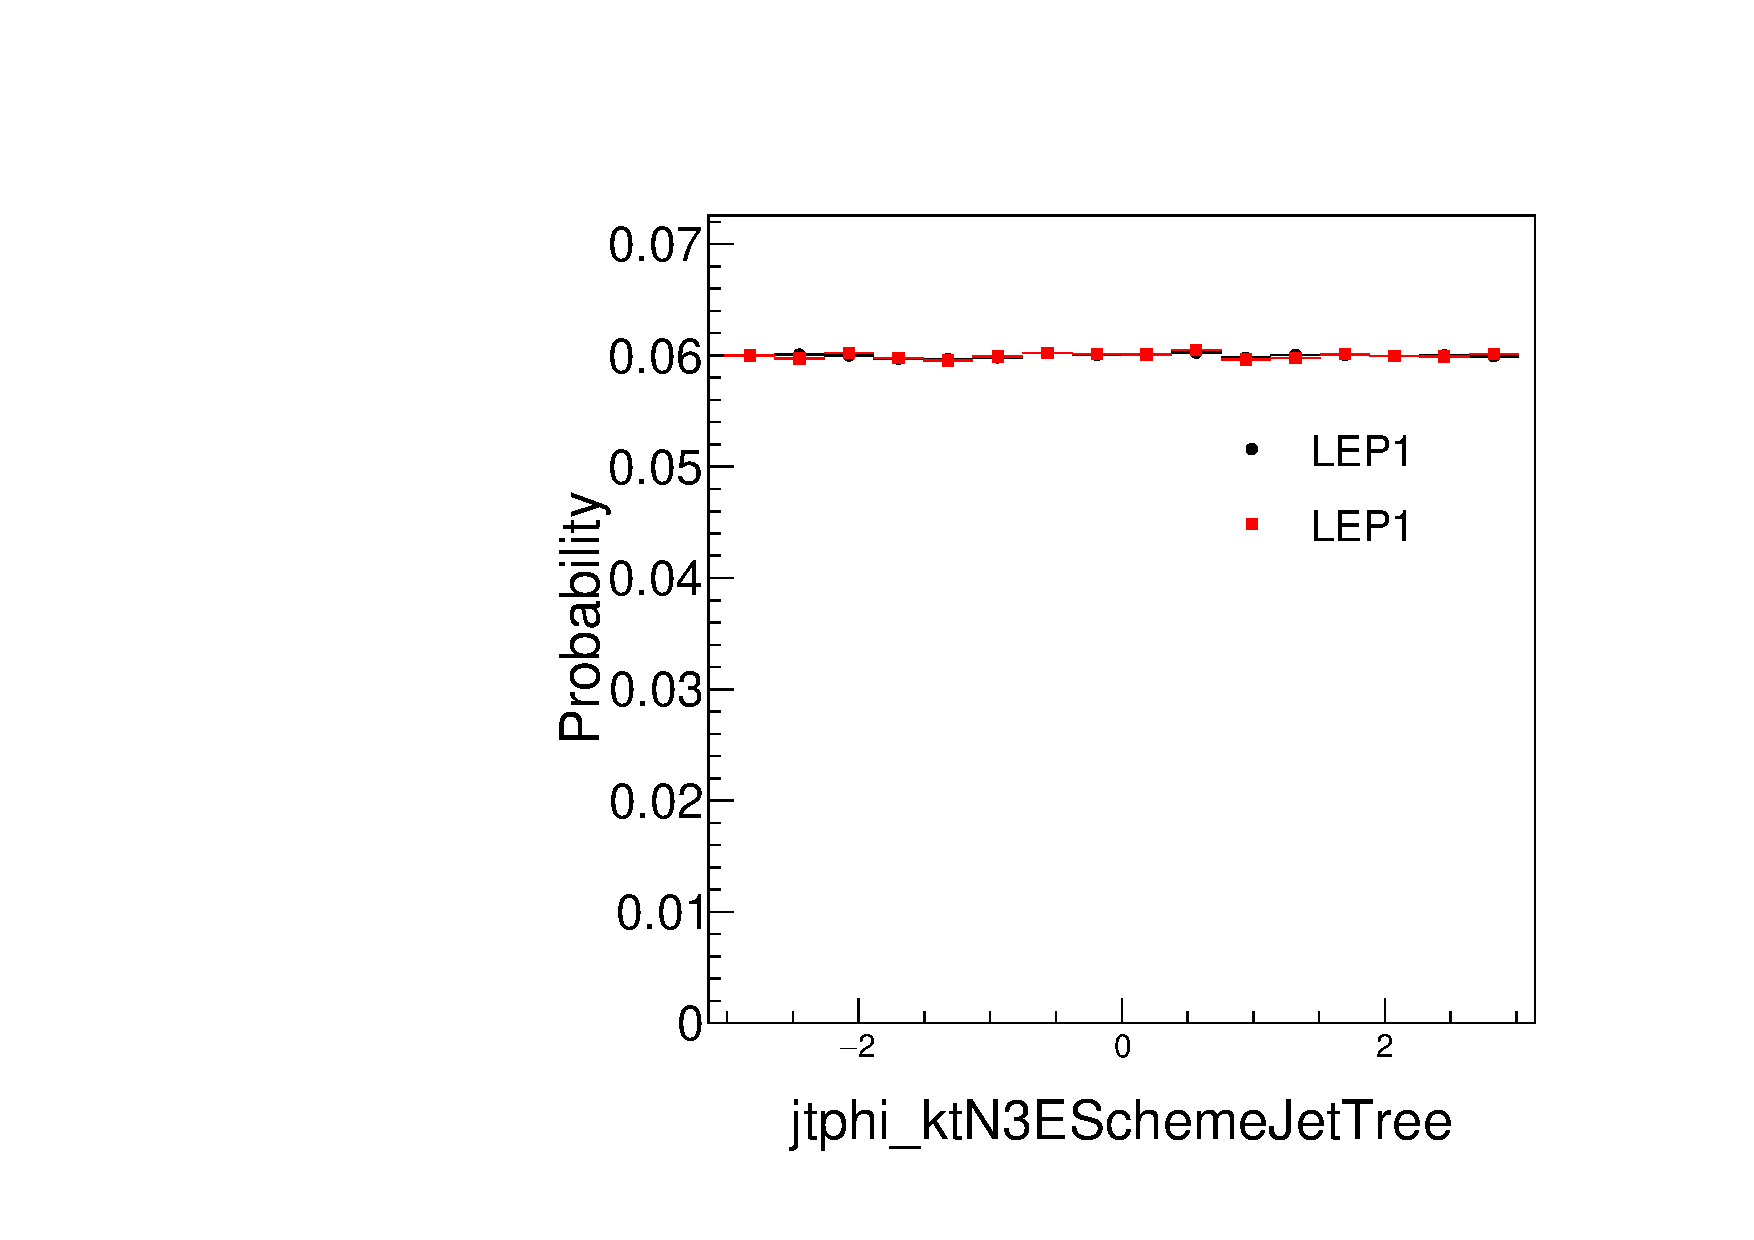
\includegraphics[width=.25\textwidth]{images/DQC/LEP1/jtphi_ktN3ESchemeJetTree.pdf}}\hfill
\subfloat{\label{sfig:g}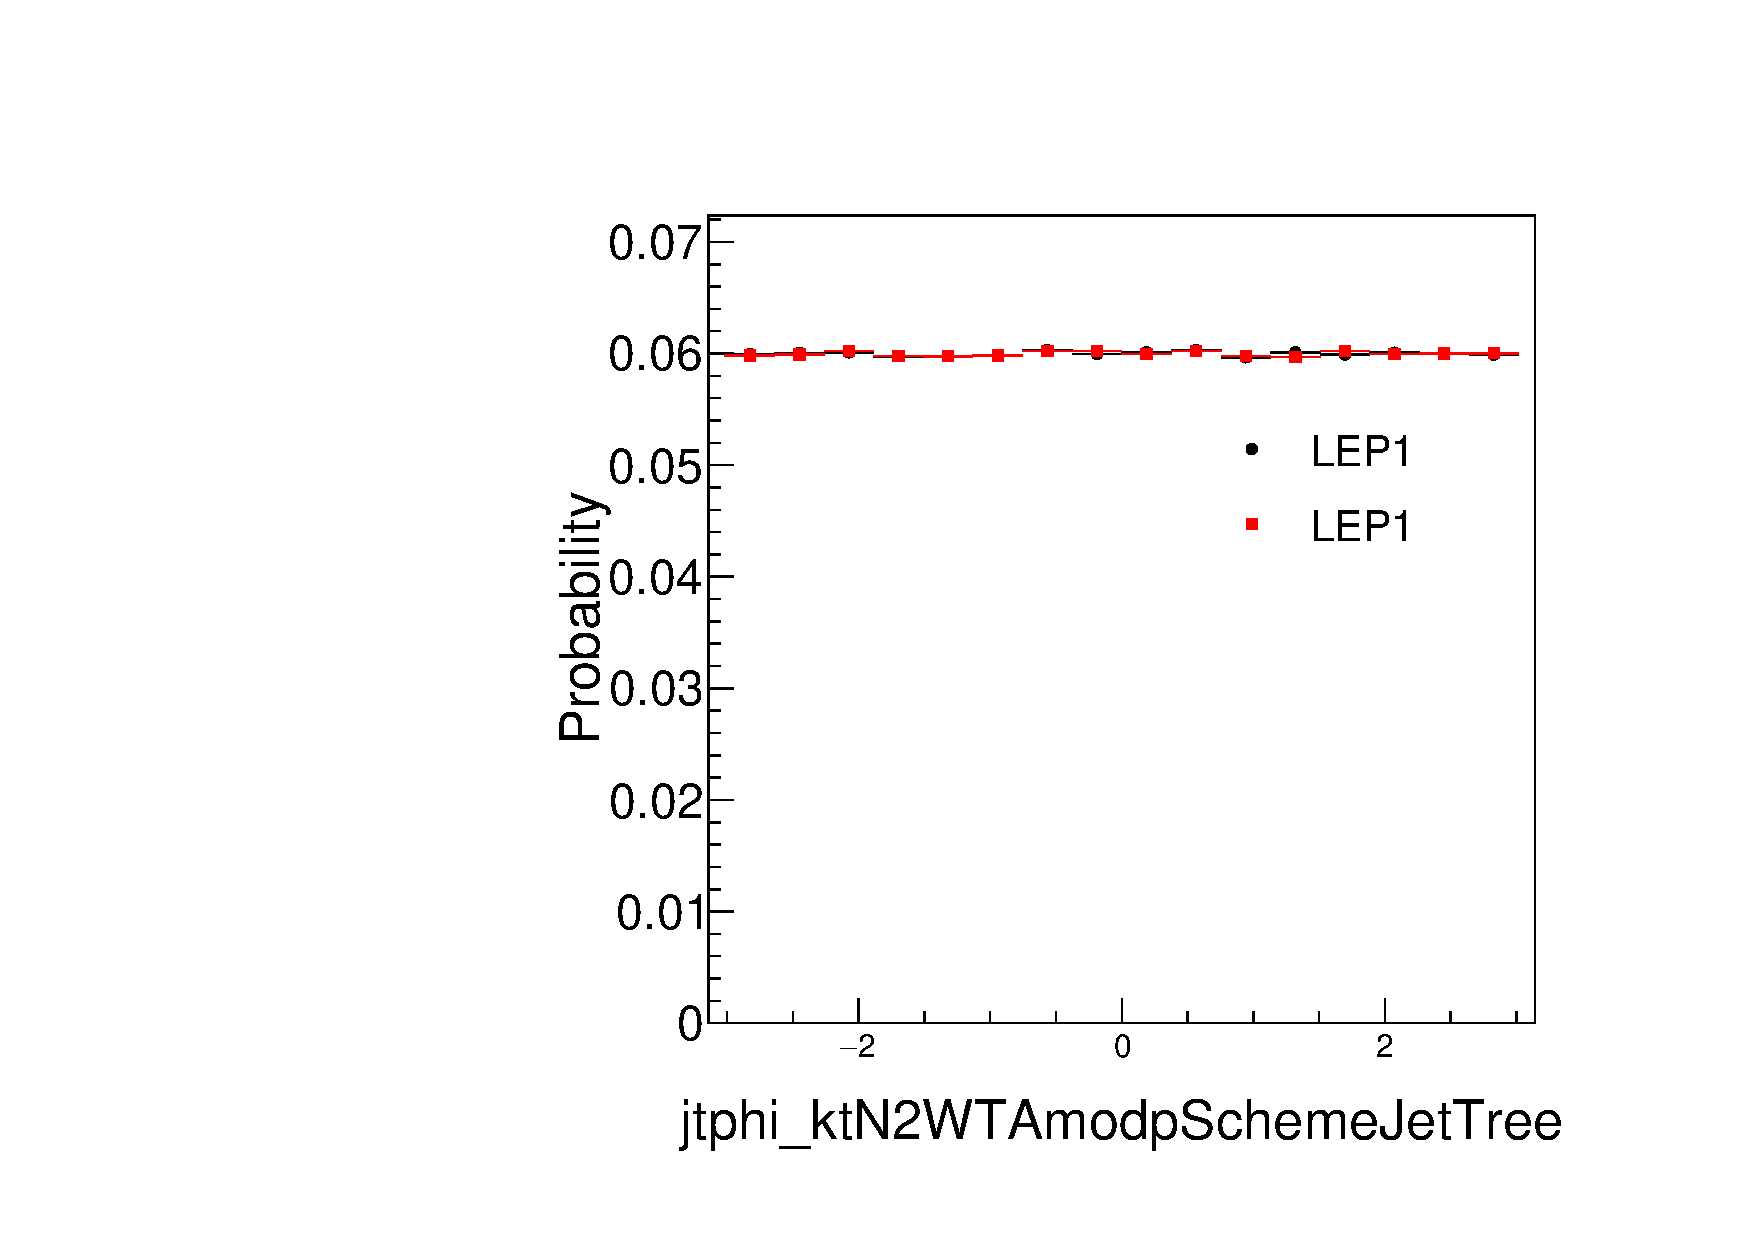
\includegraphics[width=.25\textwidth]{images/DQC/LEP1/jtphi_ktN2WTAmodpSchemeJetTree.pdf}}\hfill
\subfloat{\label{sfig:h}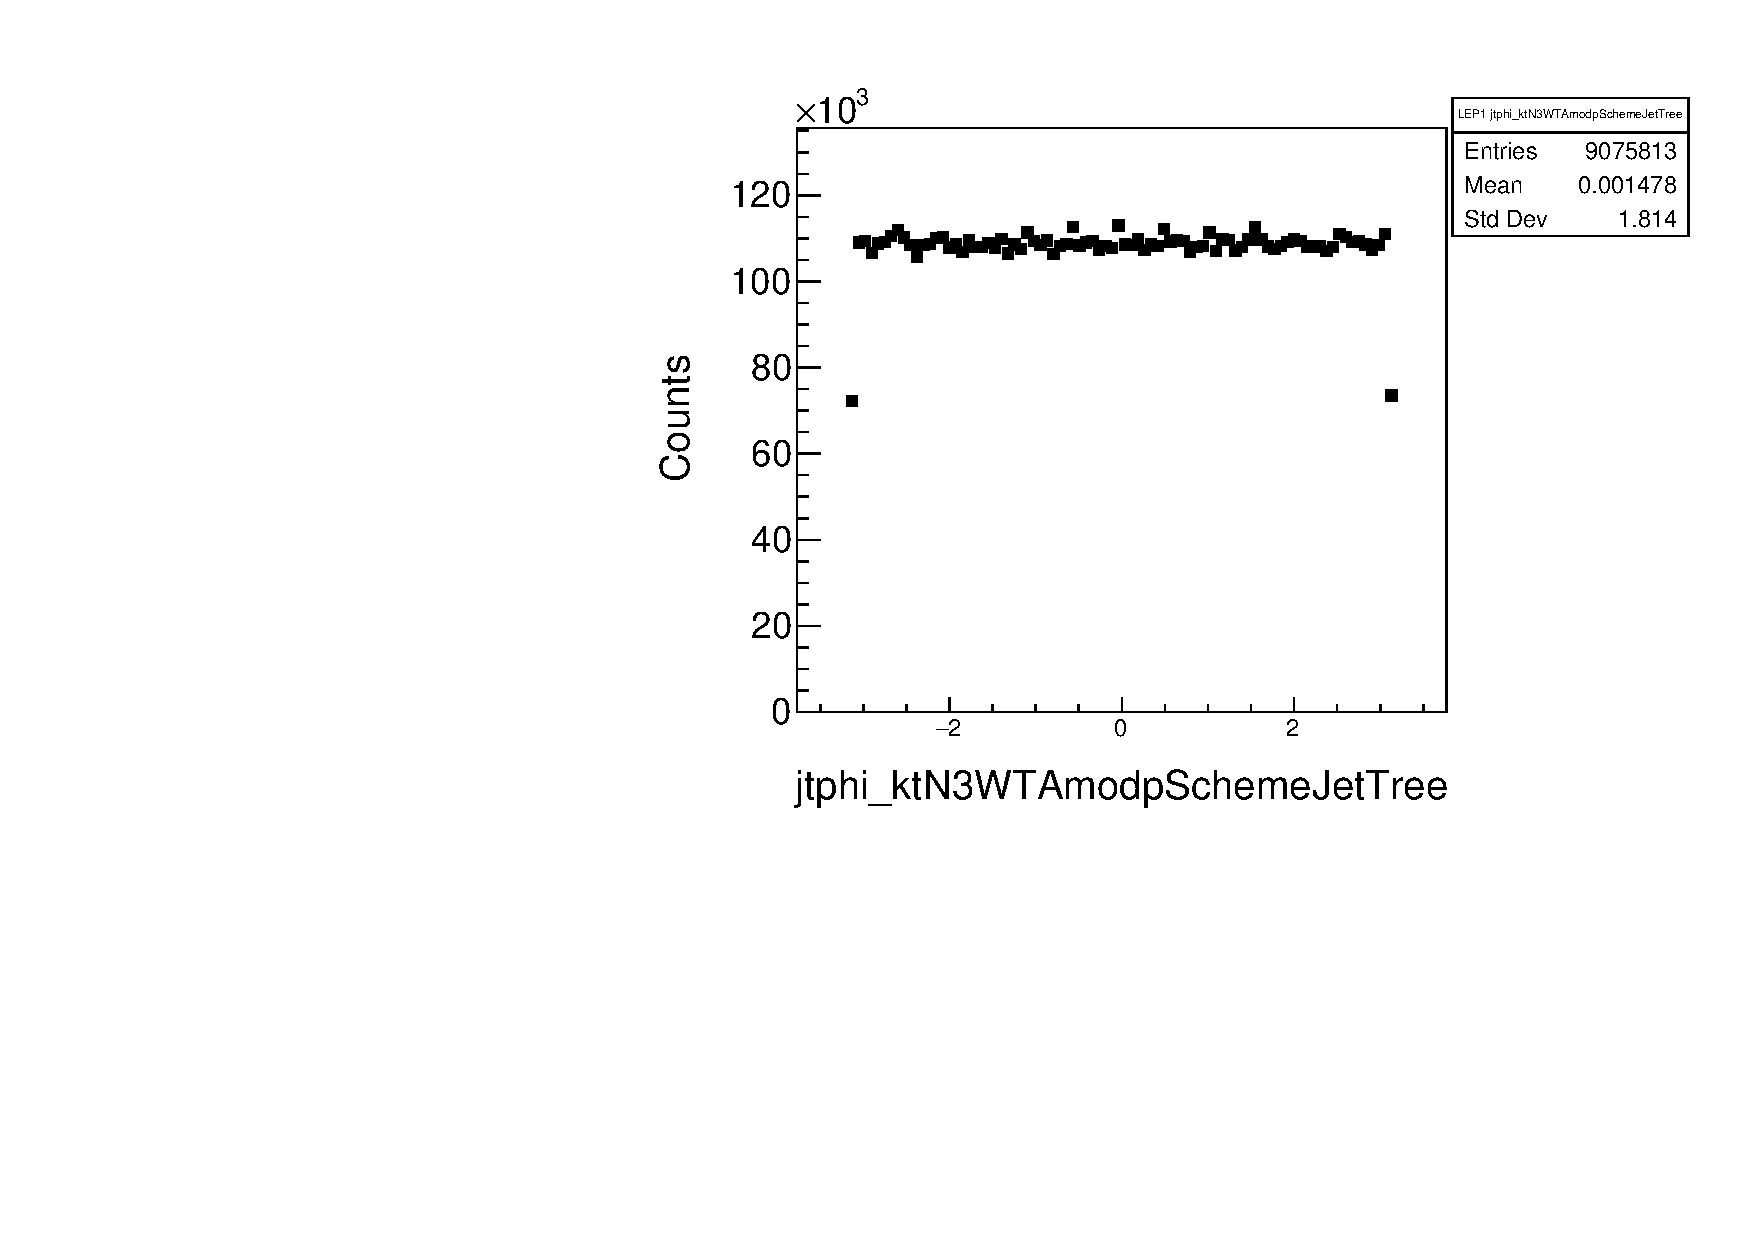
\includegraphics[width=.25\textwidth]{images/DQC/LEP1/jtphi_ktN3WTAmodpSchemeJetTree.pdf}}\hfill
\caption{LEP1 Jet $\phi$ distributions. Top row: anti-$k_t$, left to right: $R=0.4$, $E$ scheme; $R=0.8$, $E$ scheme; $R=0.4$, WTA mod p scheme; $R=0.8$, WTA mod p scheme. Bottom row: $k_t$, left to right: $N=2$, $E$ scheme; $N=3$, $E$ scheme; $N=2$, WTA mod p scheme; $N=3$; WTA mod p scheme.}  
\end{figure}

\begin{figure}[H]
\centering
\subfloat{\label{sfig:a}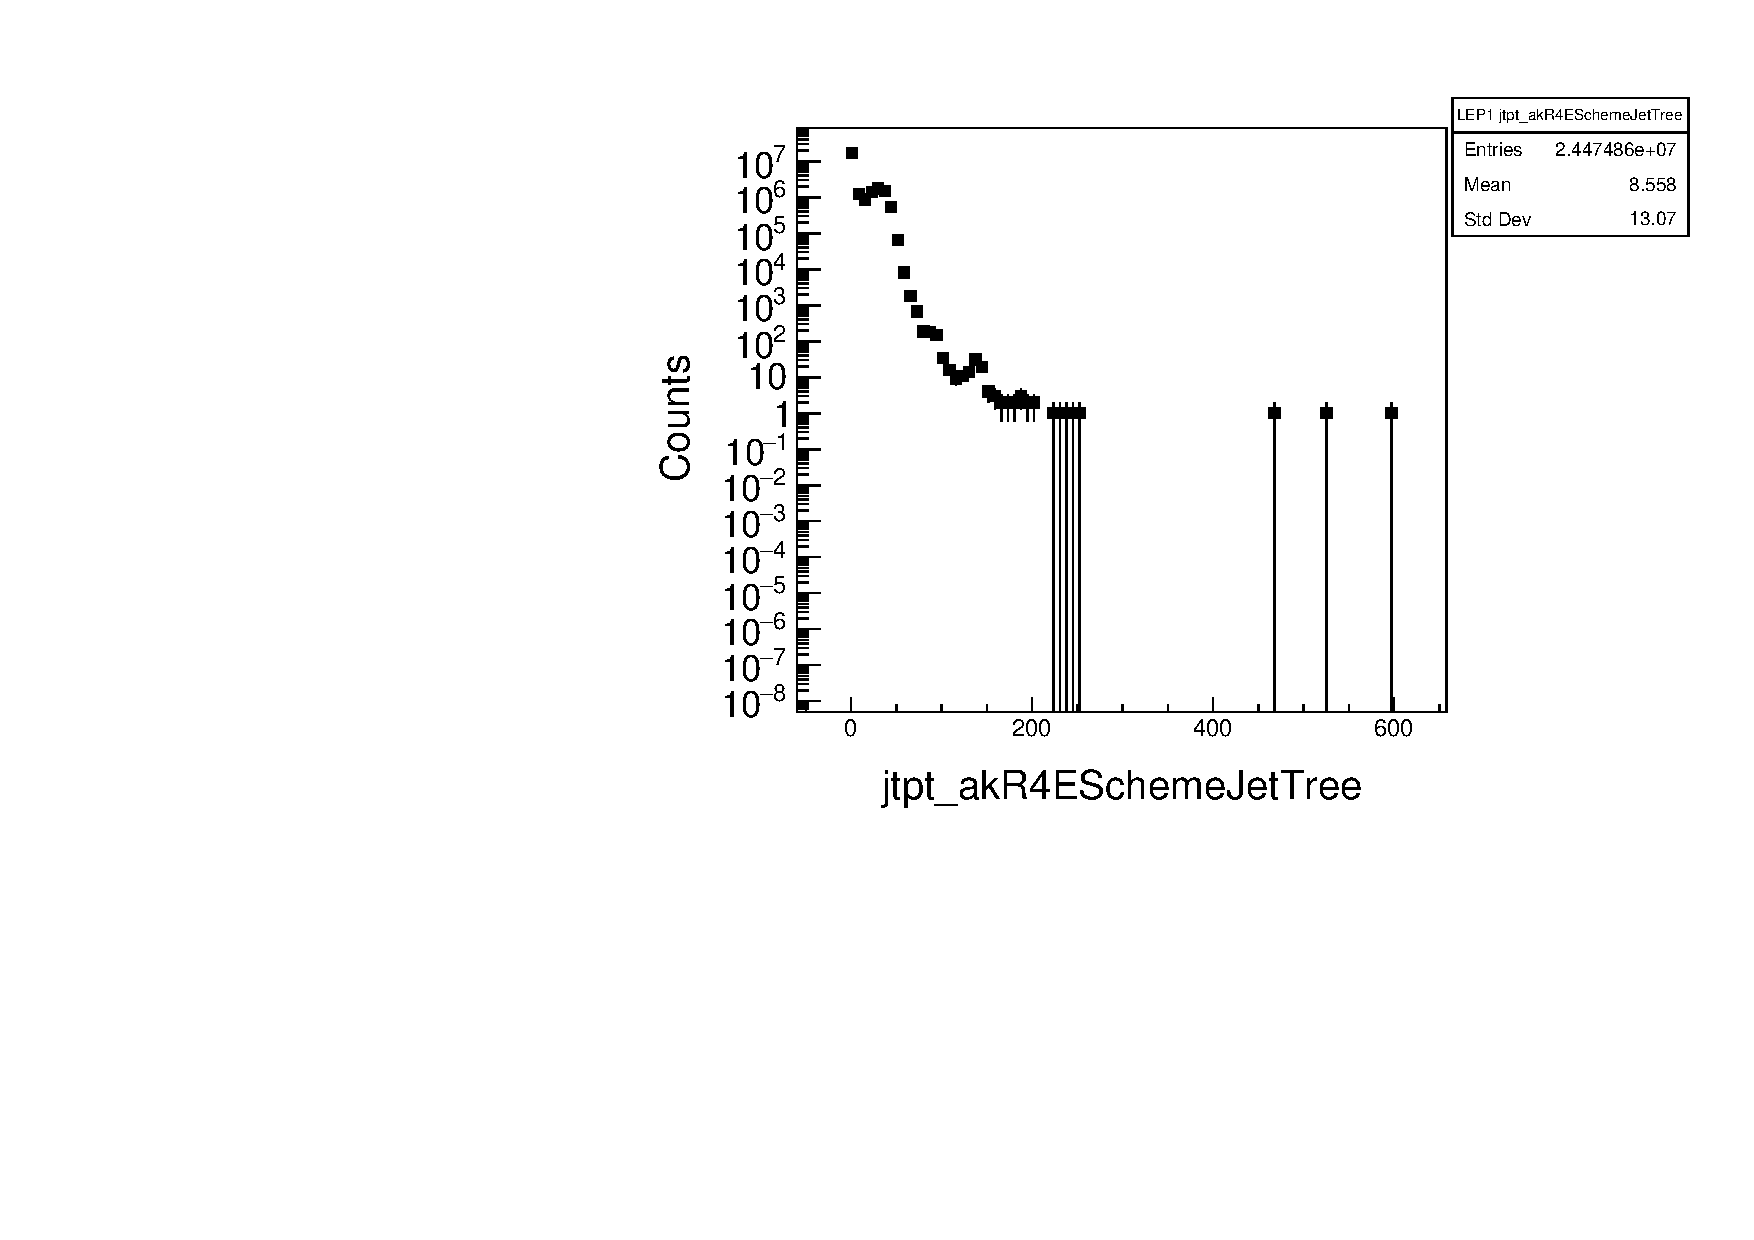
\includegraphics[width=.25\textwidth]{images/DQC/LEP1/jtpt_akR4ESchemeJetTree.pdf}}\hfill
\subfloat{\label{sfig:b}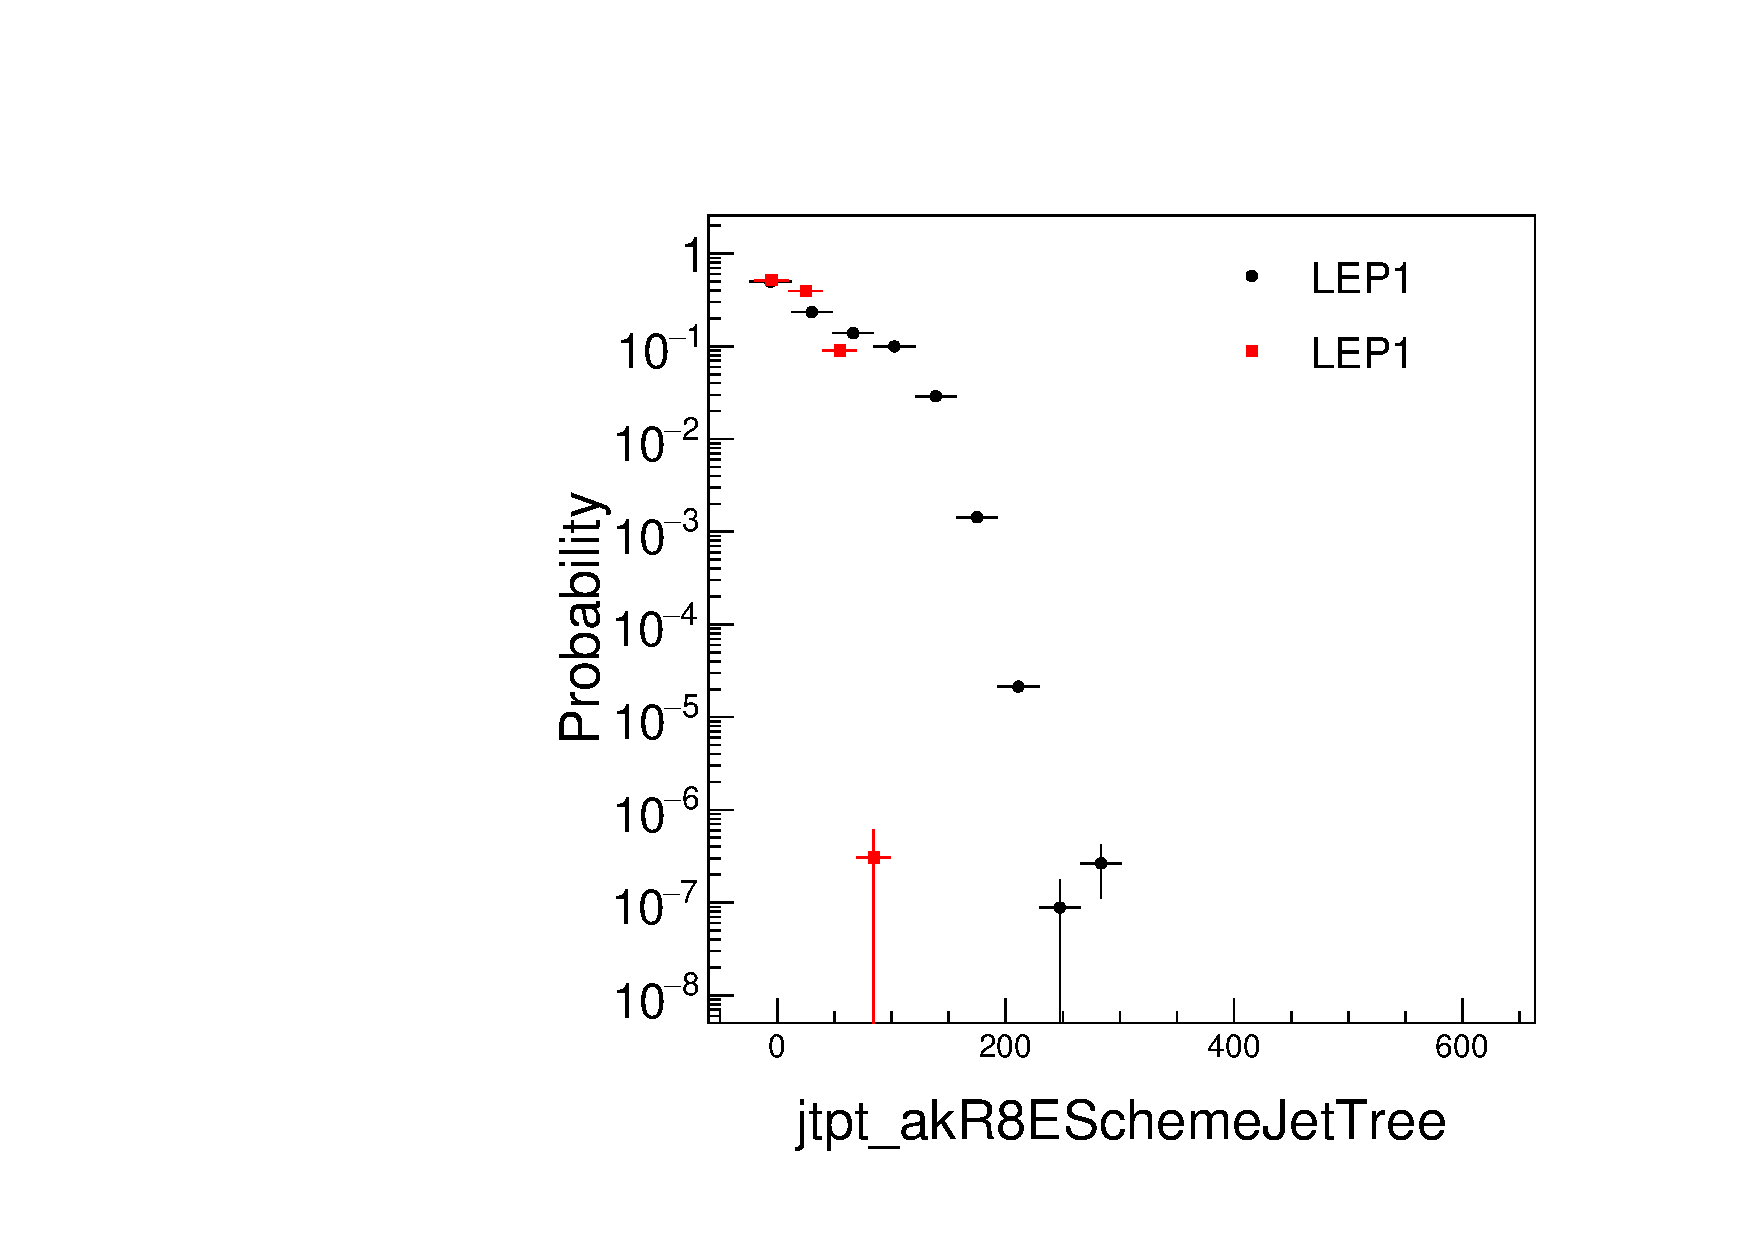
\includegraphics[width=.25\textwidth]{images/DQC/LEP1/jtpt_akR8ESchemeJetTree.pdf}}\hfill
\subfloat{\label{sfig:c}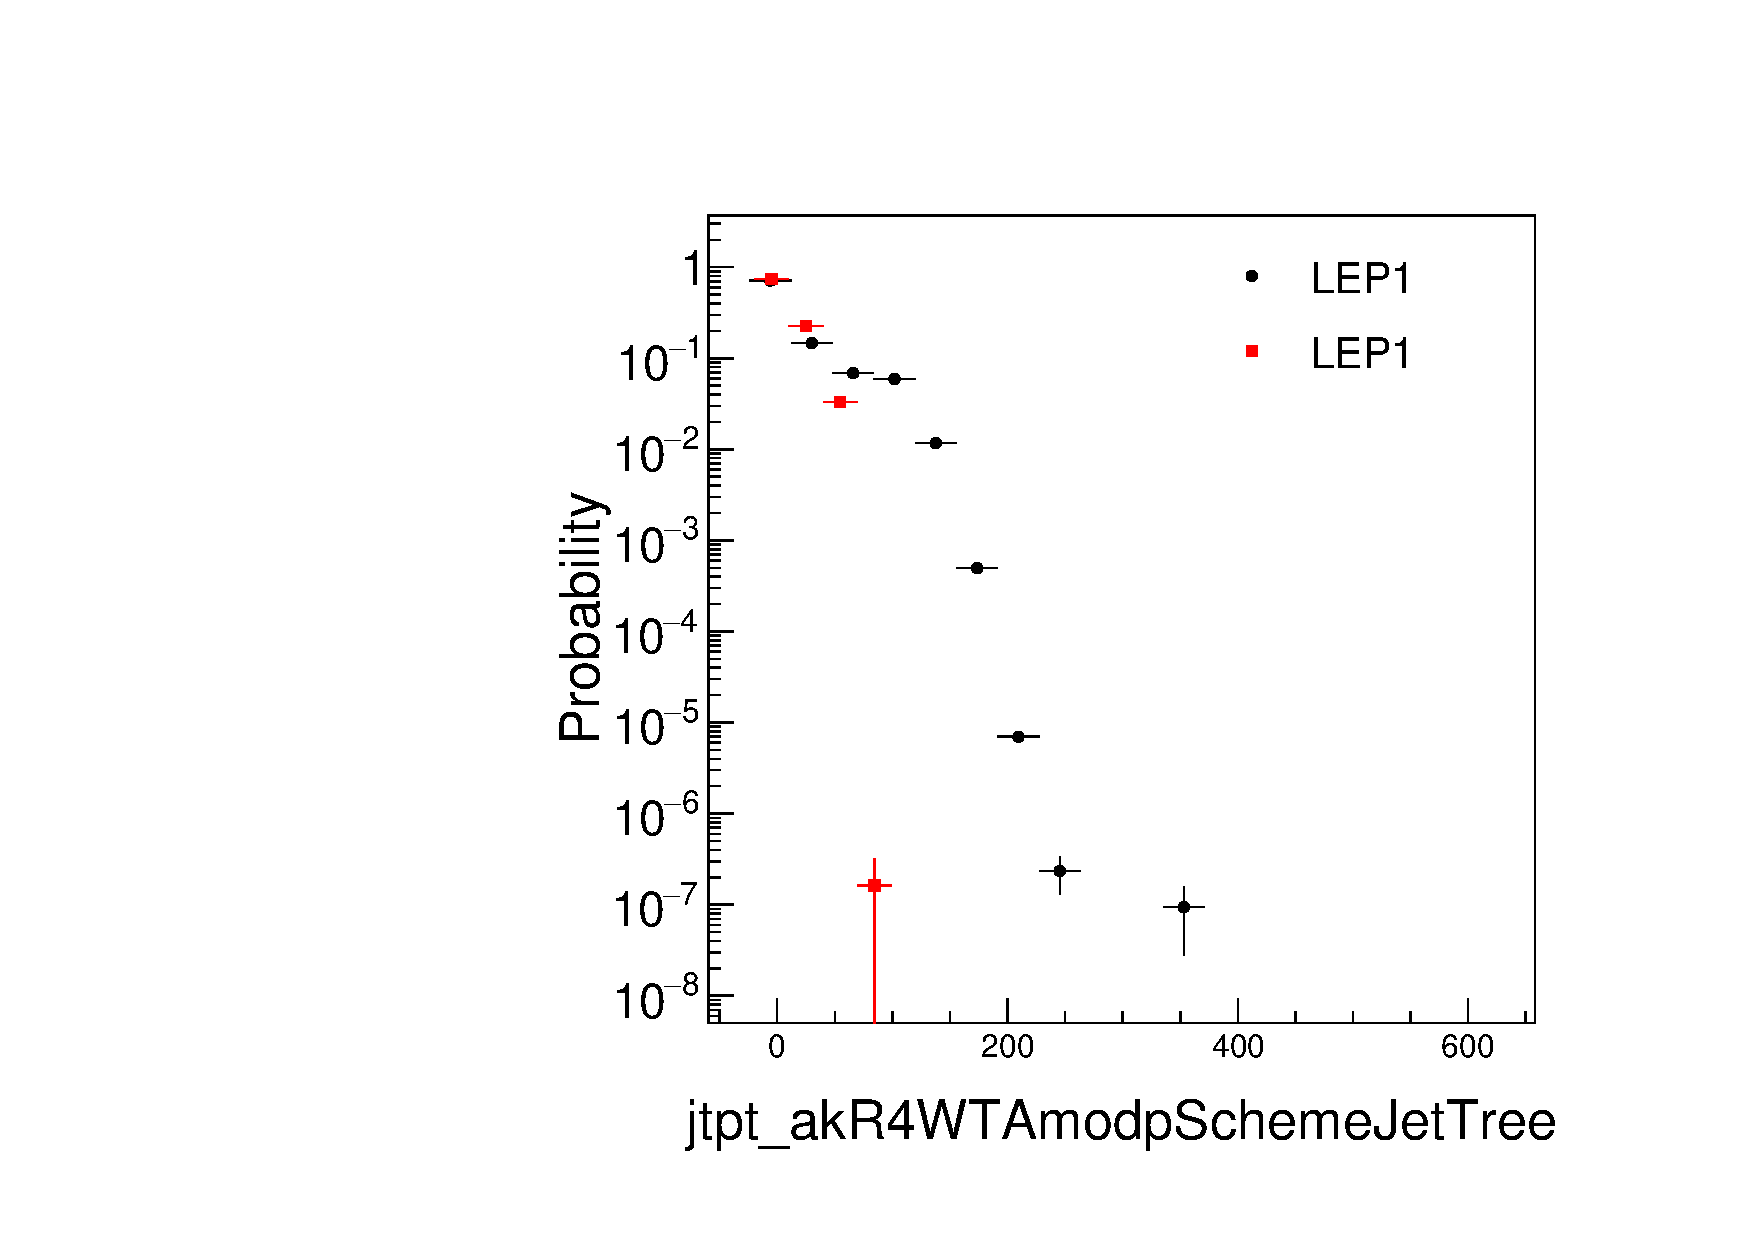
\includegraphics[width=.25\textwidth]{images/DQC/LEP1/jtpt_akR4WTAmodpSchemeJetTree.pdf}}\hfill
\subfloat{\label{sfig:d}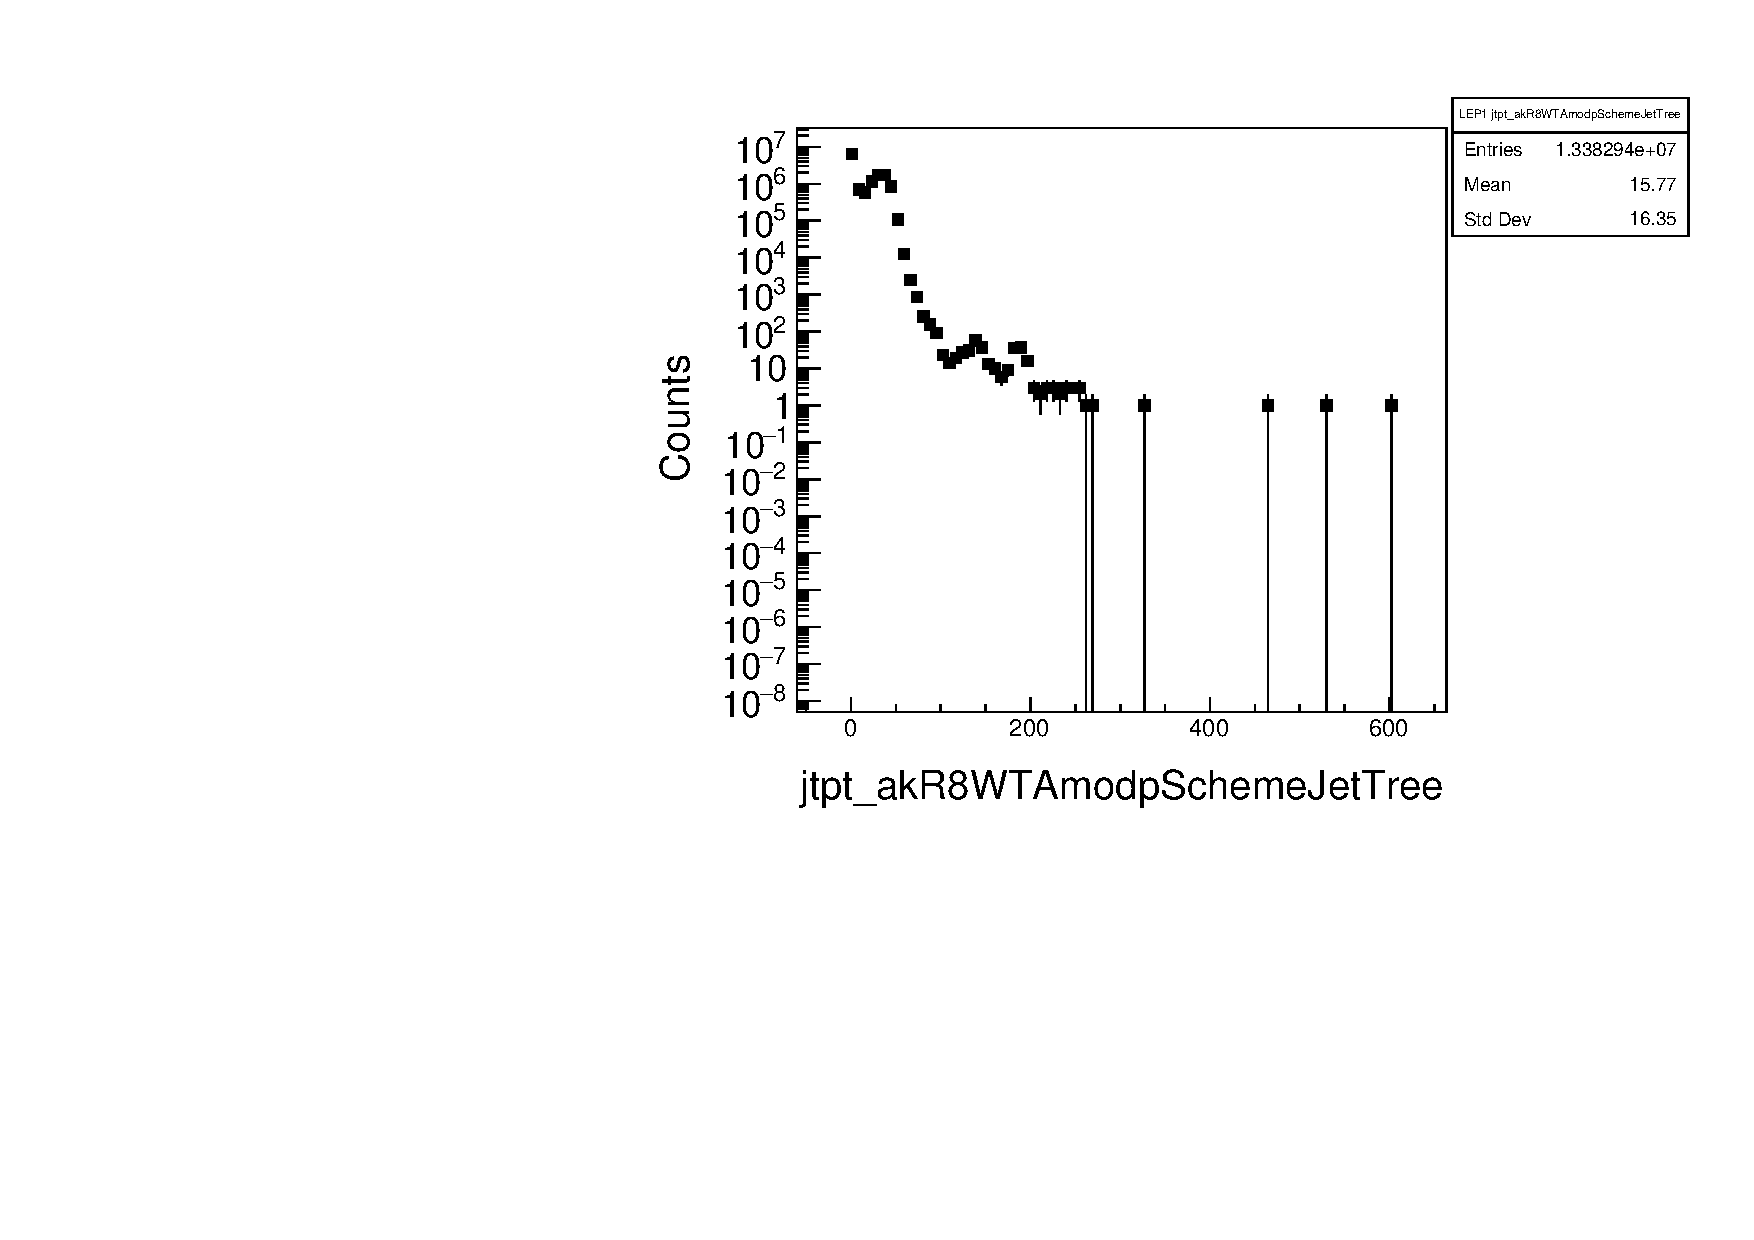
\includegraphics[width=.25\textwidth]{images/DQC/LEP1/jtpt_akR8WTAmodpSchemeJetTree.pdf}}\hfill %row end
\subfloat{\label{sfig:e}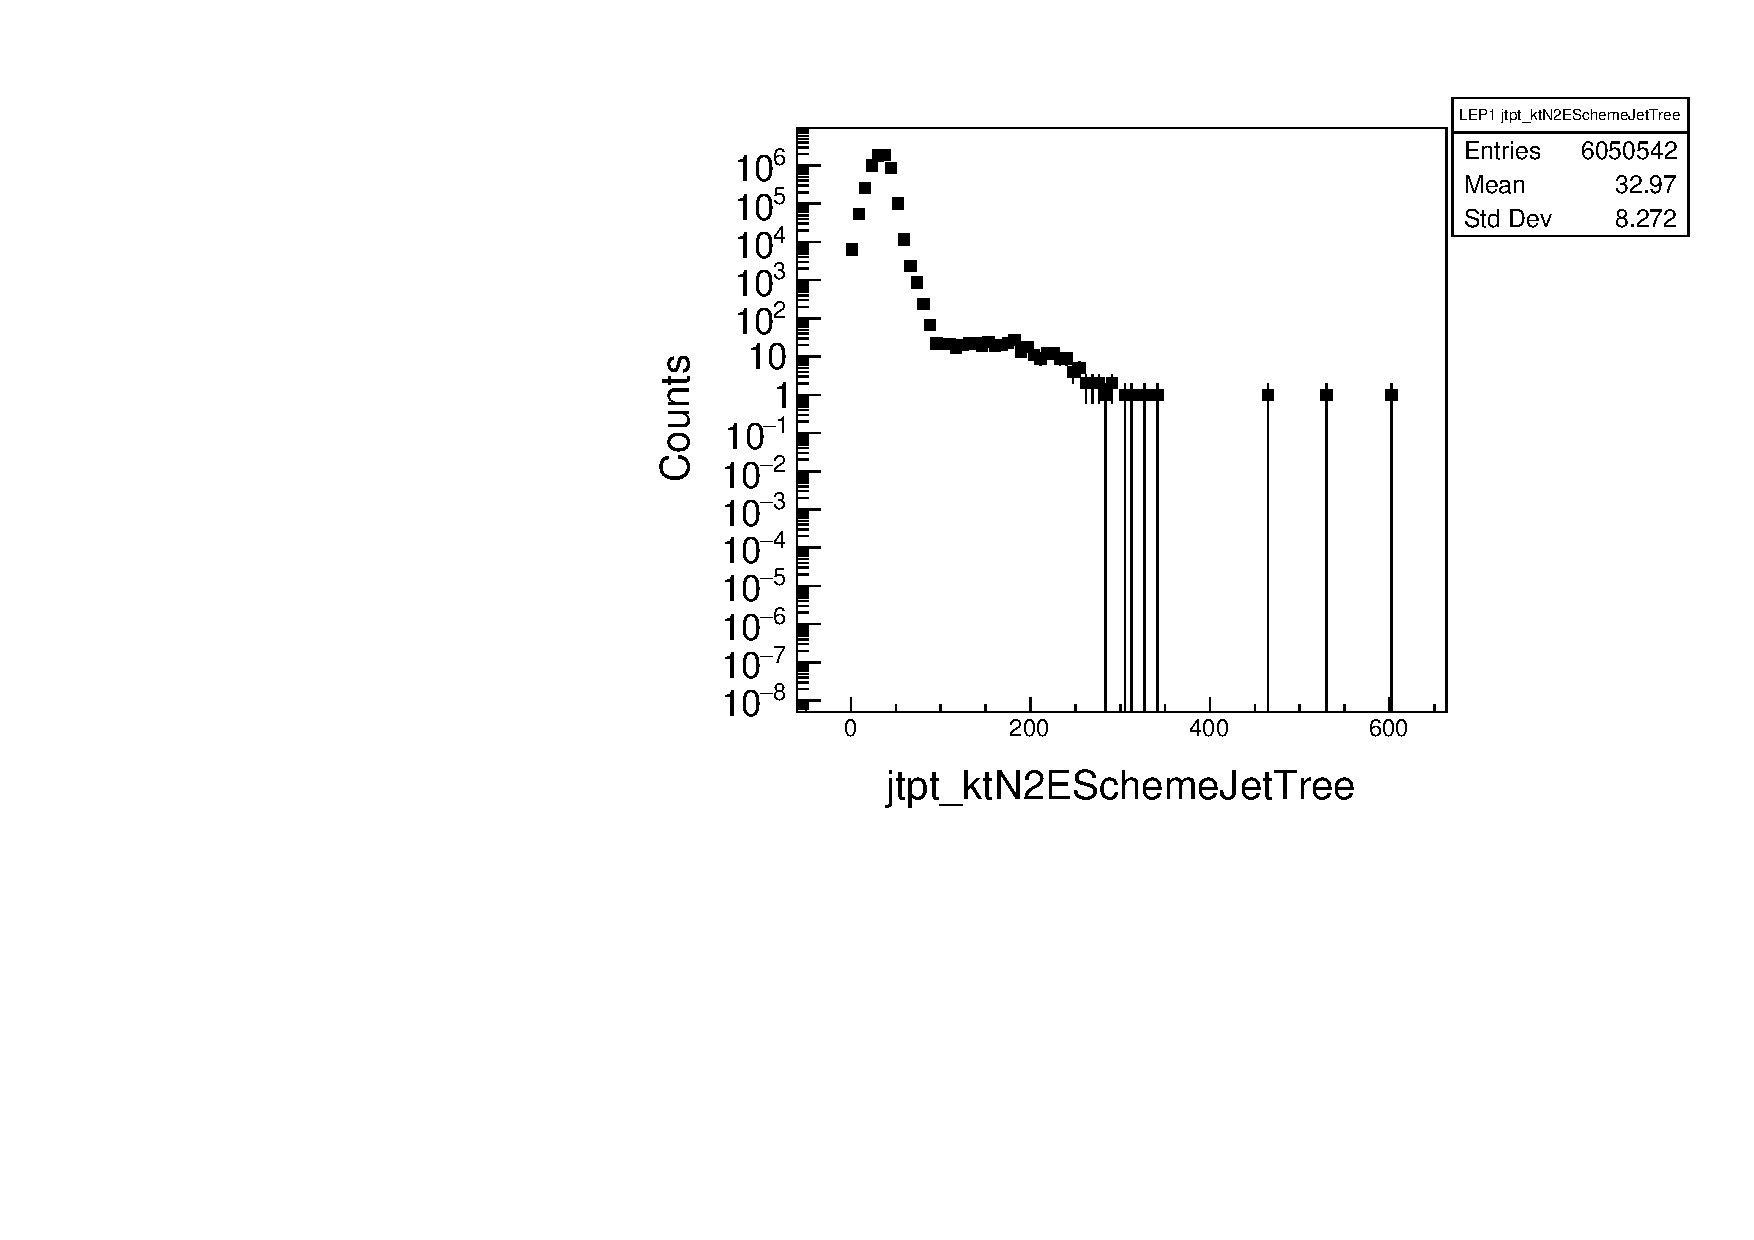
\includegraphics[width=.25\textwidth]{images/DQC/LEP1/jtpt_ktN2ESchemeJetTree.pdf}}\hfill
\subfloat{\label{sfig:f}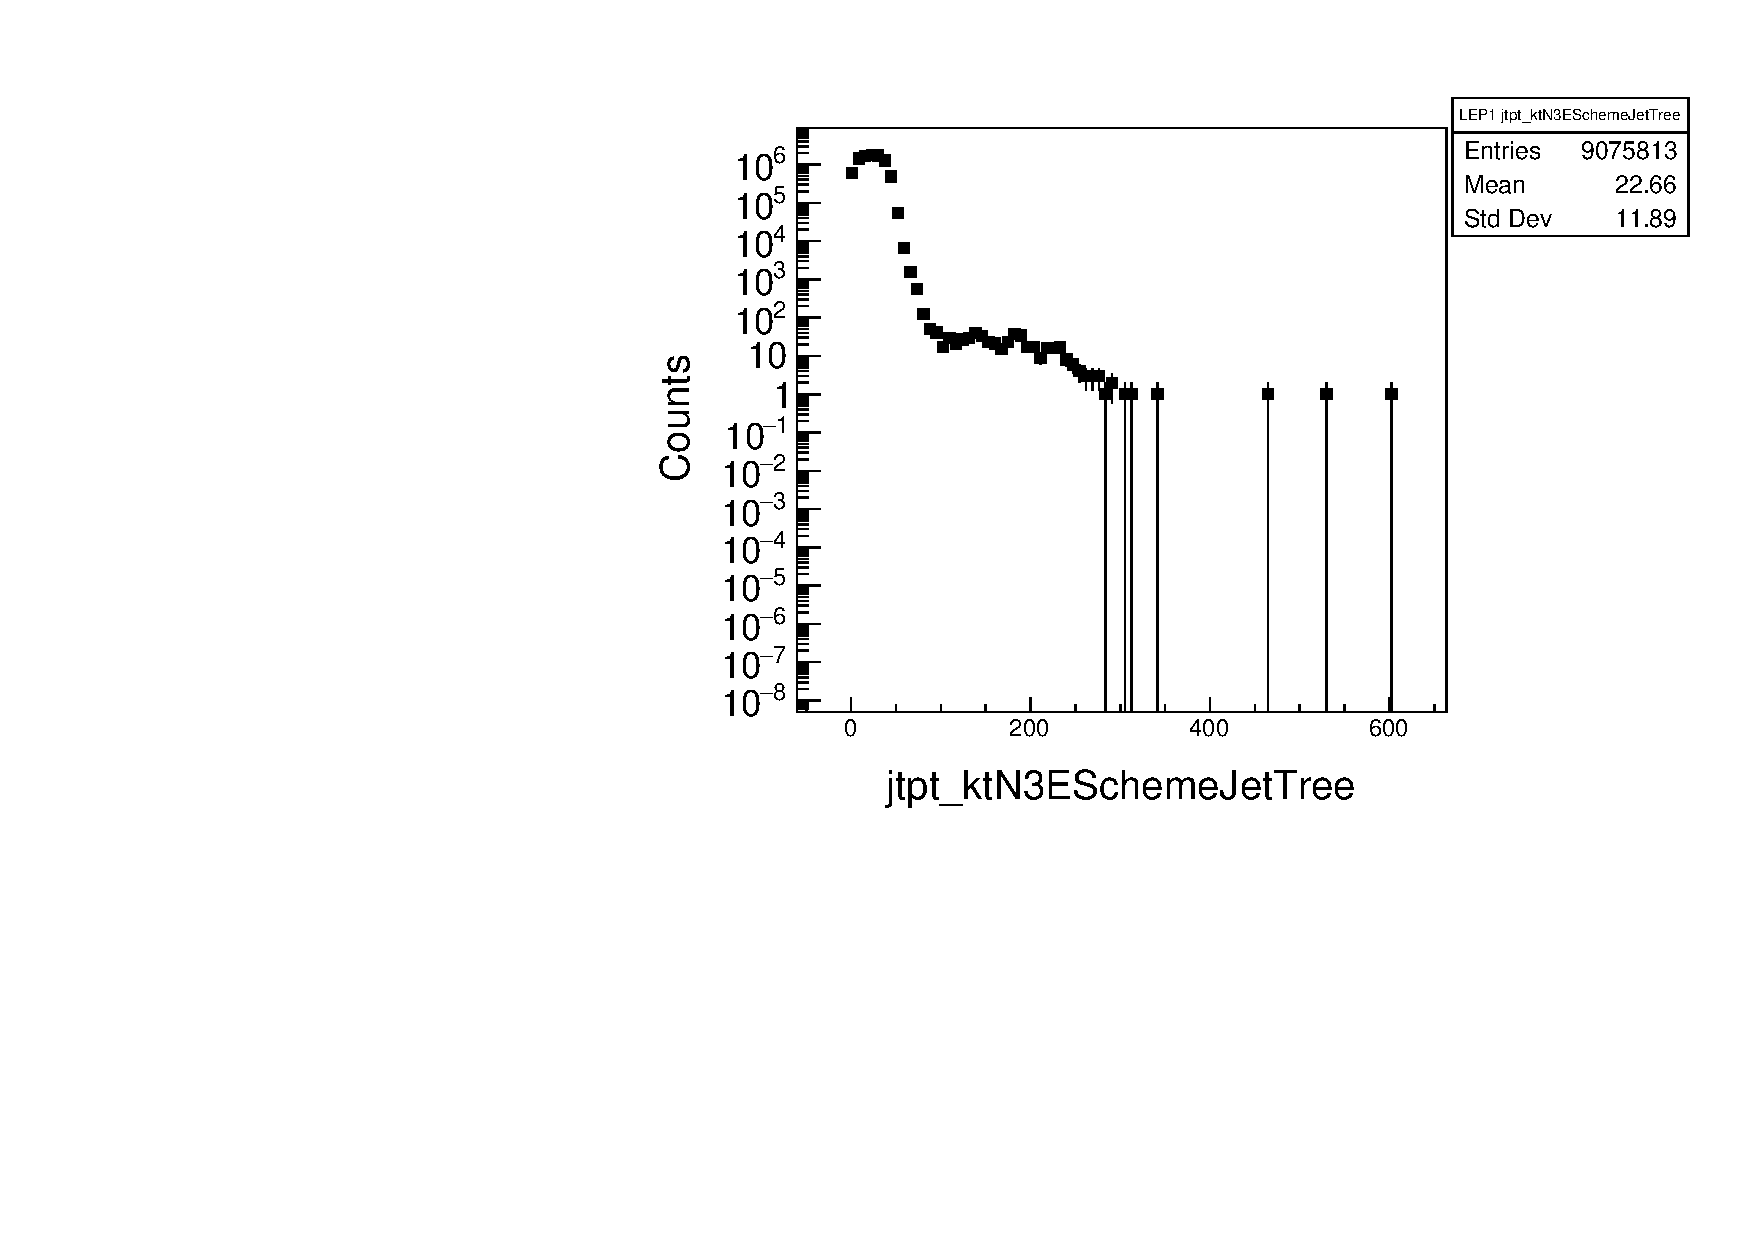
\includegraphics[width=.25\textwidth]{images/DQC/LEP1/jtpt_ktN3ESchemeJetTree.pdf}}\hfill
\subfloat{\label{sfig:g}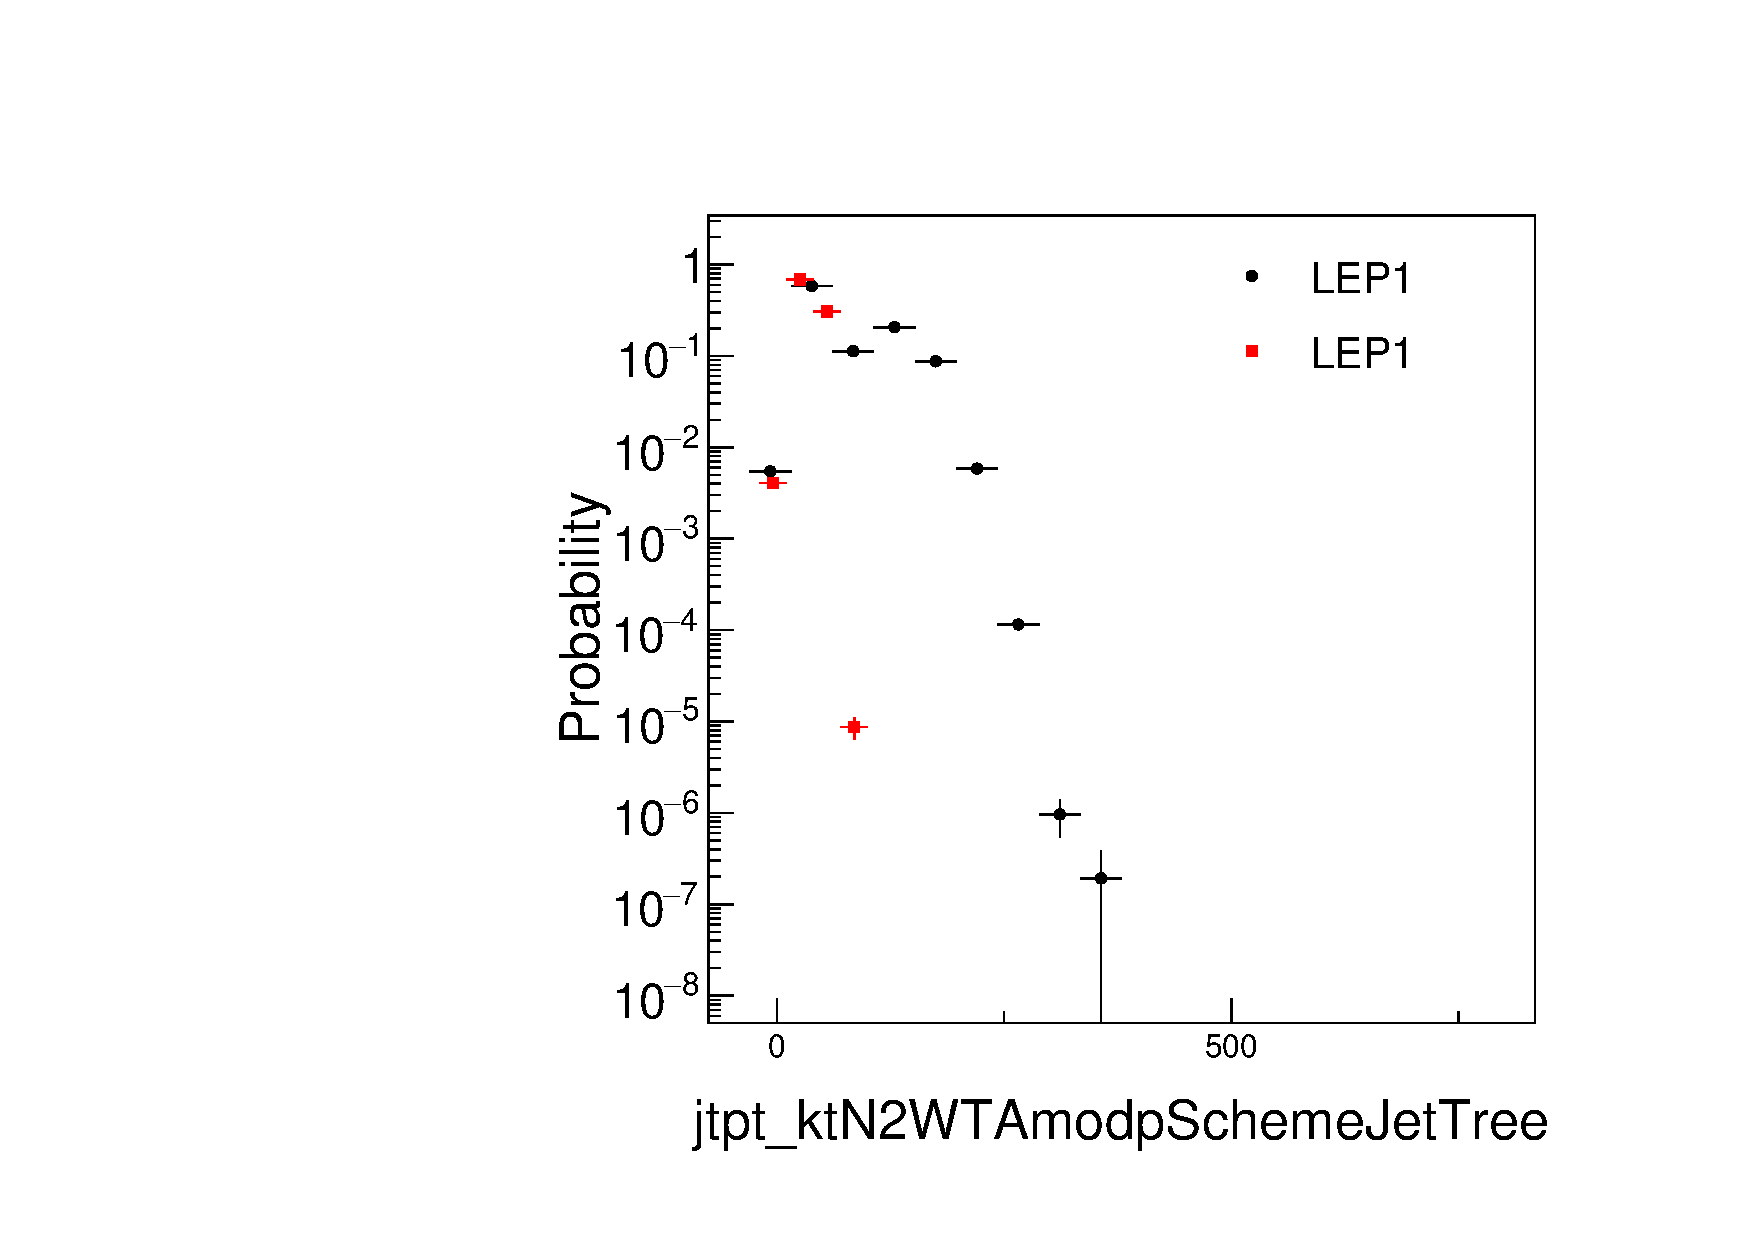
\includegraphics[width=.25\textwidth]{images/DQC/LEP1/jtpt_ktN2WTAmodpSchemeJetTree.pdf}}\hfill
\subfloat{\label{sfig:h}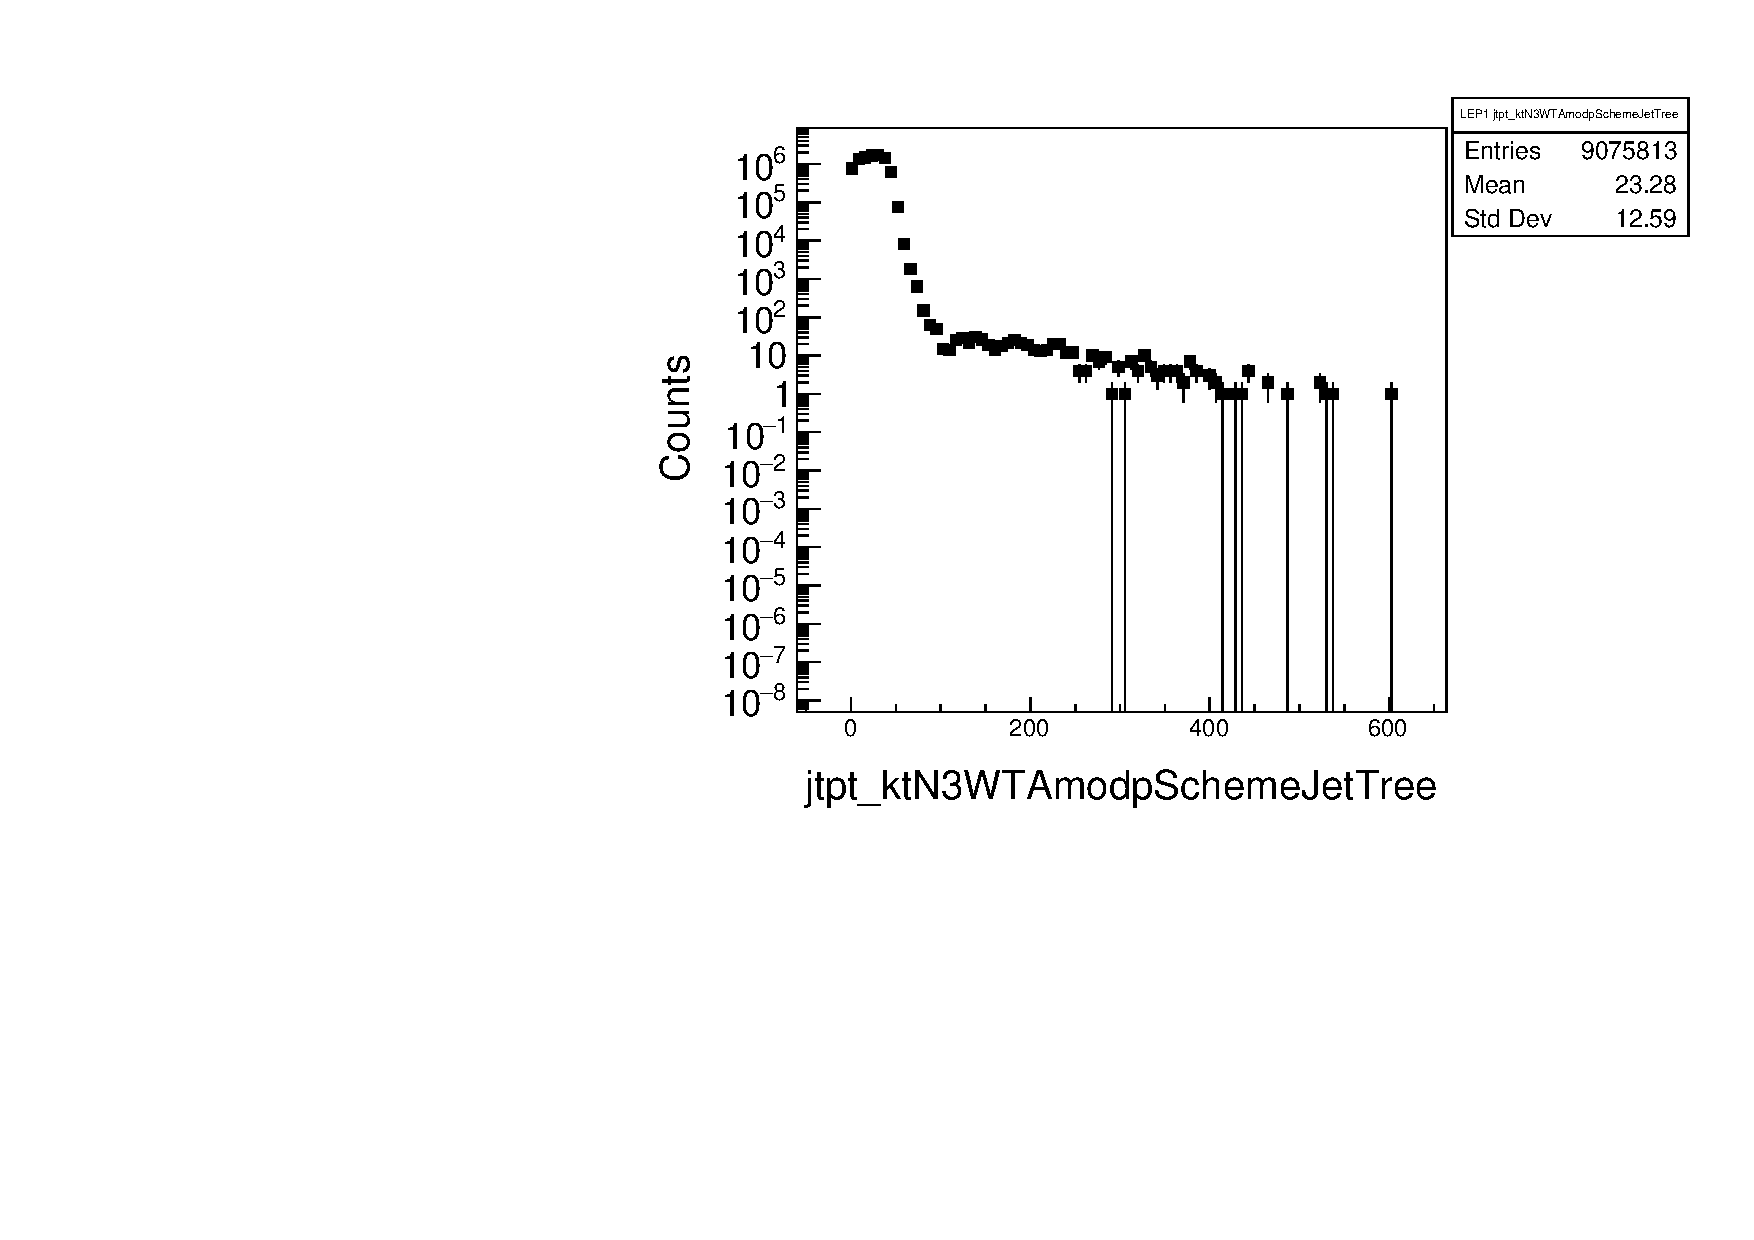
\includegraphics[width=.25\textwidth]{images/DQC/LEP1/jtpt_ktN3WTAmodpSchemeJetTree.pdf}}\hfill
\caption{LEP1 Jet $p_t$ distributions. Top row: anti-$k_t$, left to right: $R=0.4$, $E$ scheme; $R=0.8$, $E$ scheme; $R=0.4$, WTA mod p scheme; $R=0.8$, WTA mod p scheme. Bottom row: $k_t$, left to right: $N=2$, $E$ scheme; $N=3$, $E$ scheme; $N=2$, WTA mod p scheme; $N=3$; WTA mod p scheme.}  
\end{figure}

\begin{figure}[H]
\centering
\subfloat{\label{sfig:a}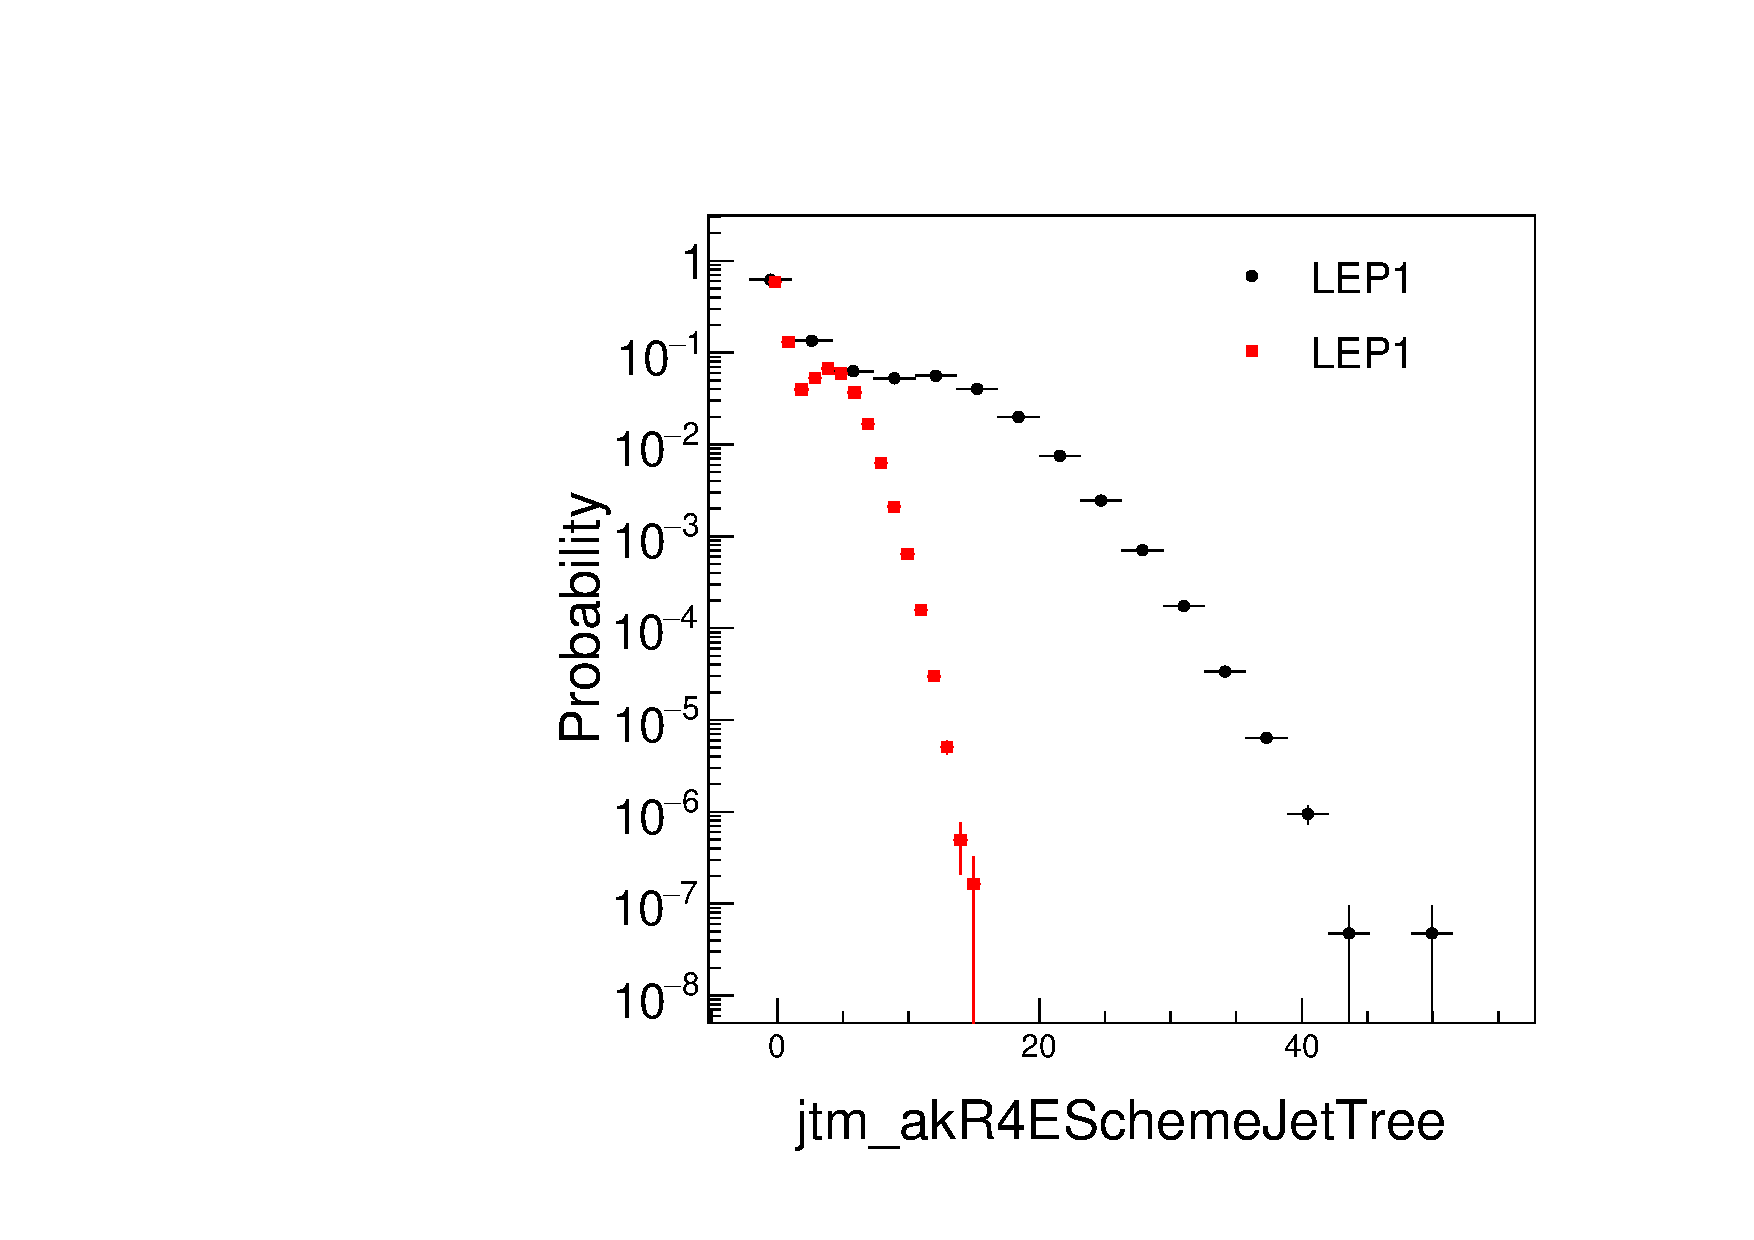
\includegraphics[width=.25\textwidth]{images/DQC/LEP1/jtm_akR4ESchemeJetTree.pdf}}\hfill
\subfloat{\label{sfig:b}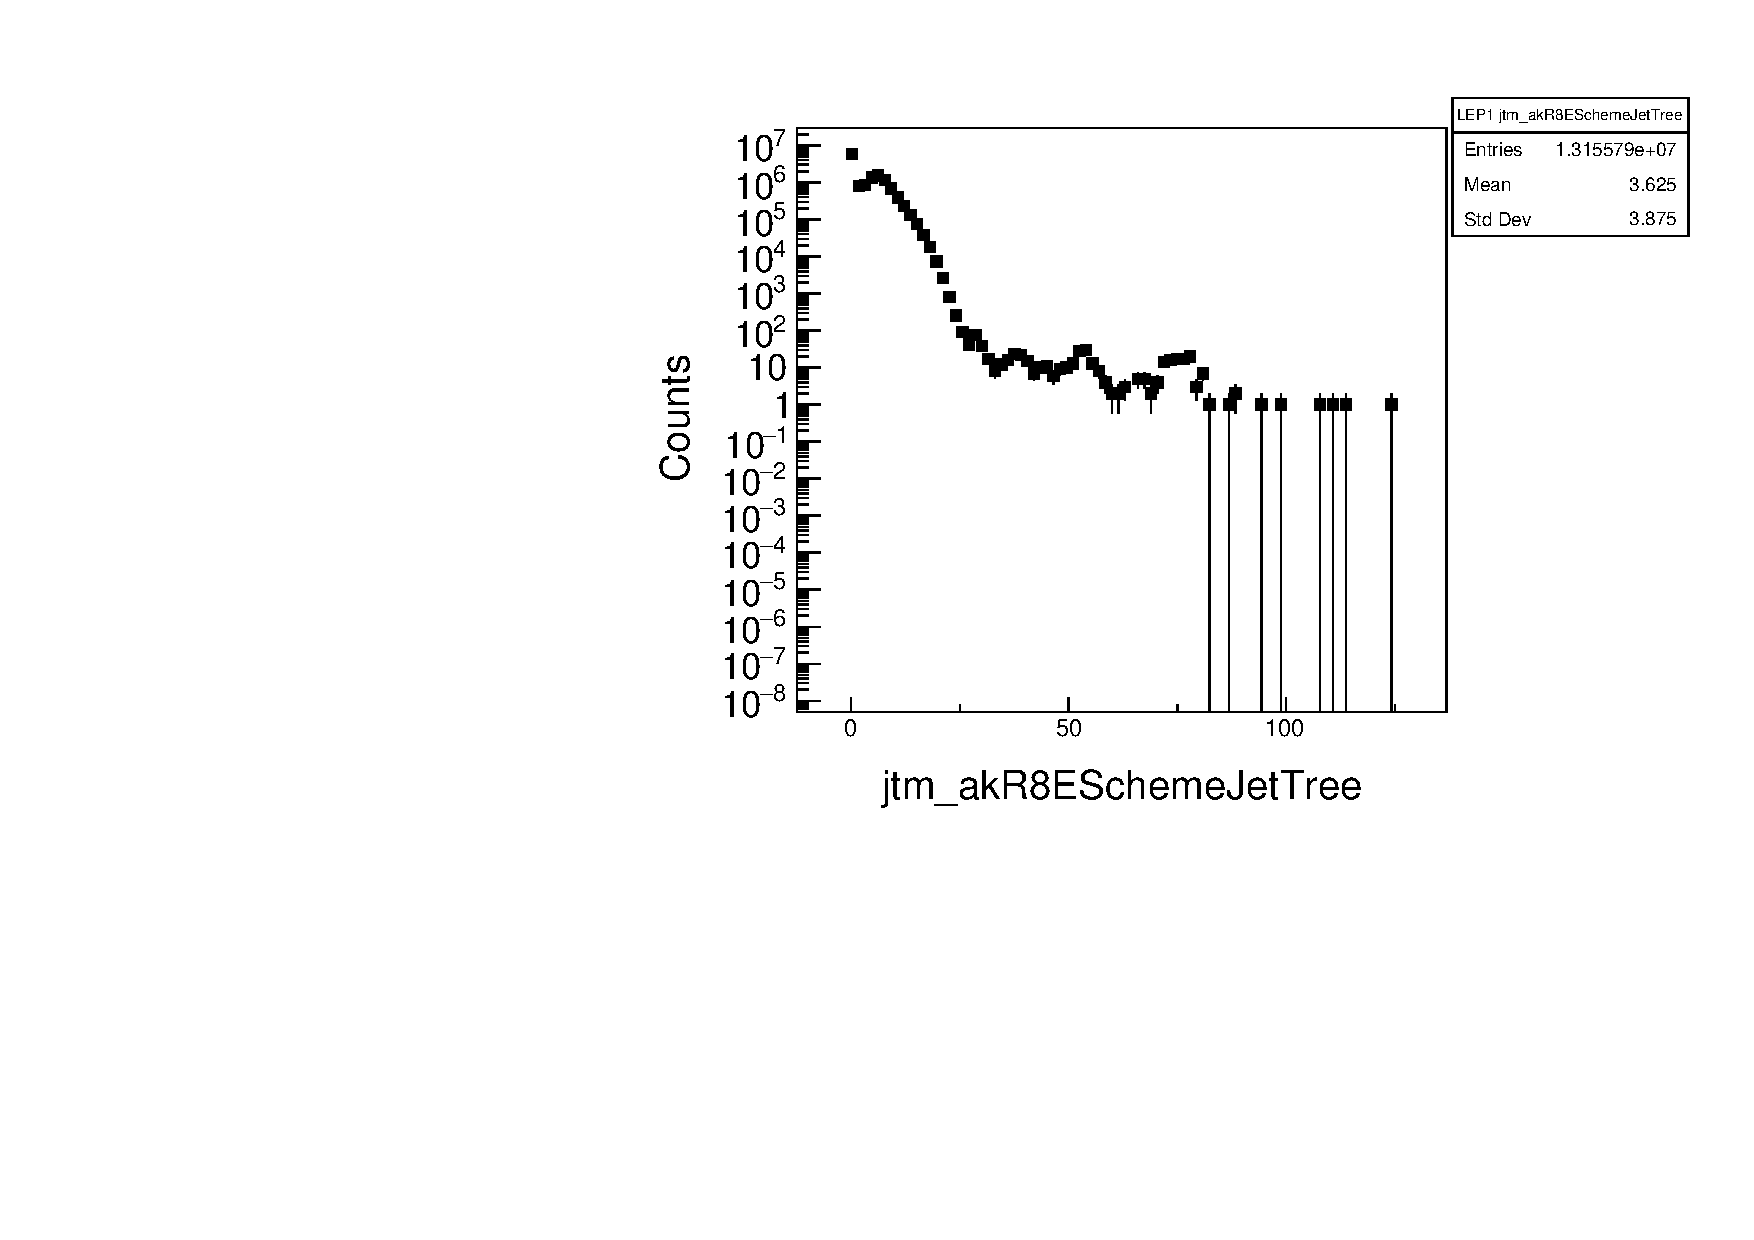
\includegraphics[width=.25\textwidth]{images/DQC/LEP1/jtm_akR8ESchemeJetTree.pdf}}\hfill
\subfloat{\label{sfig:c}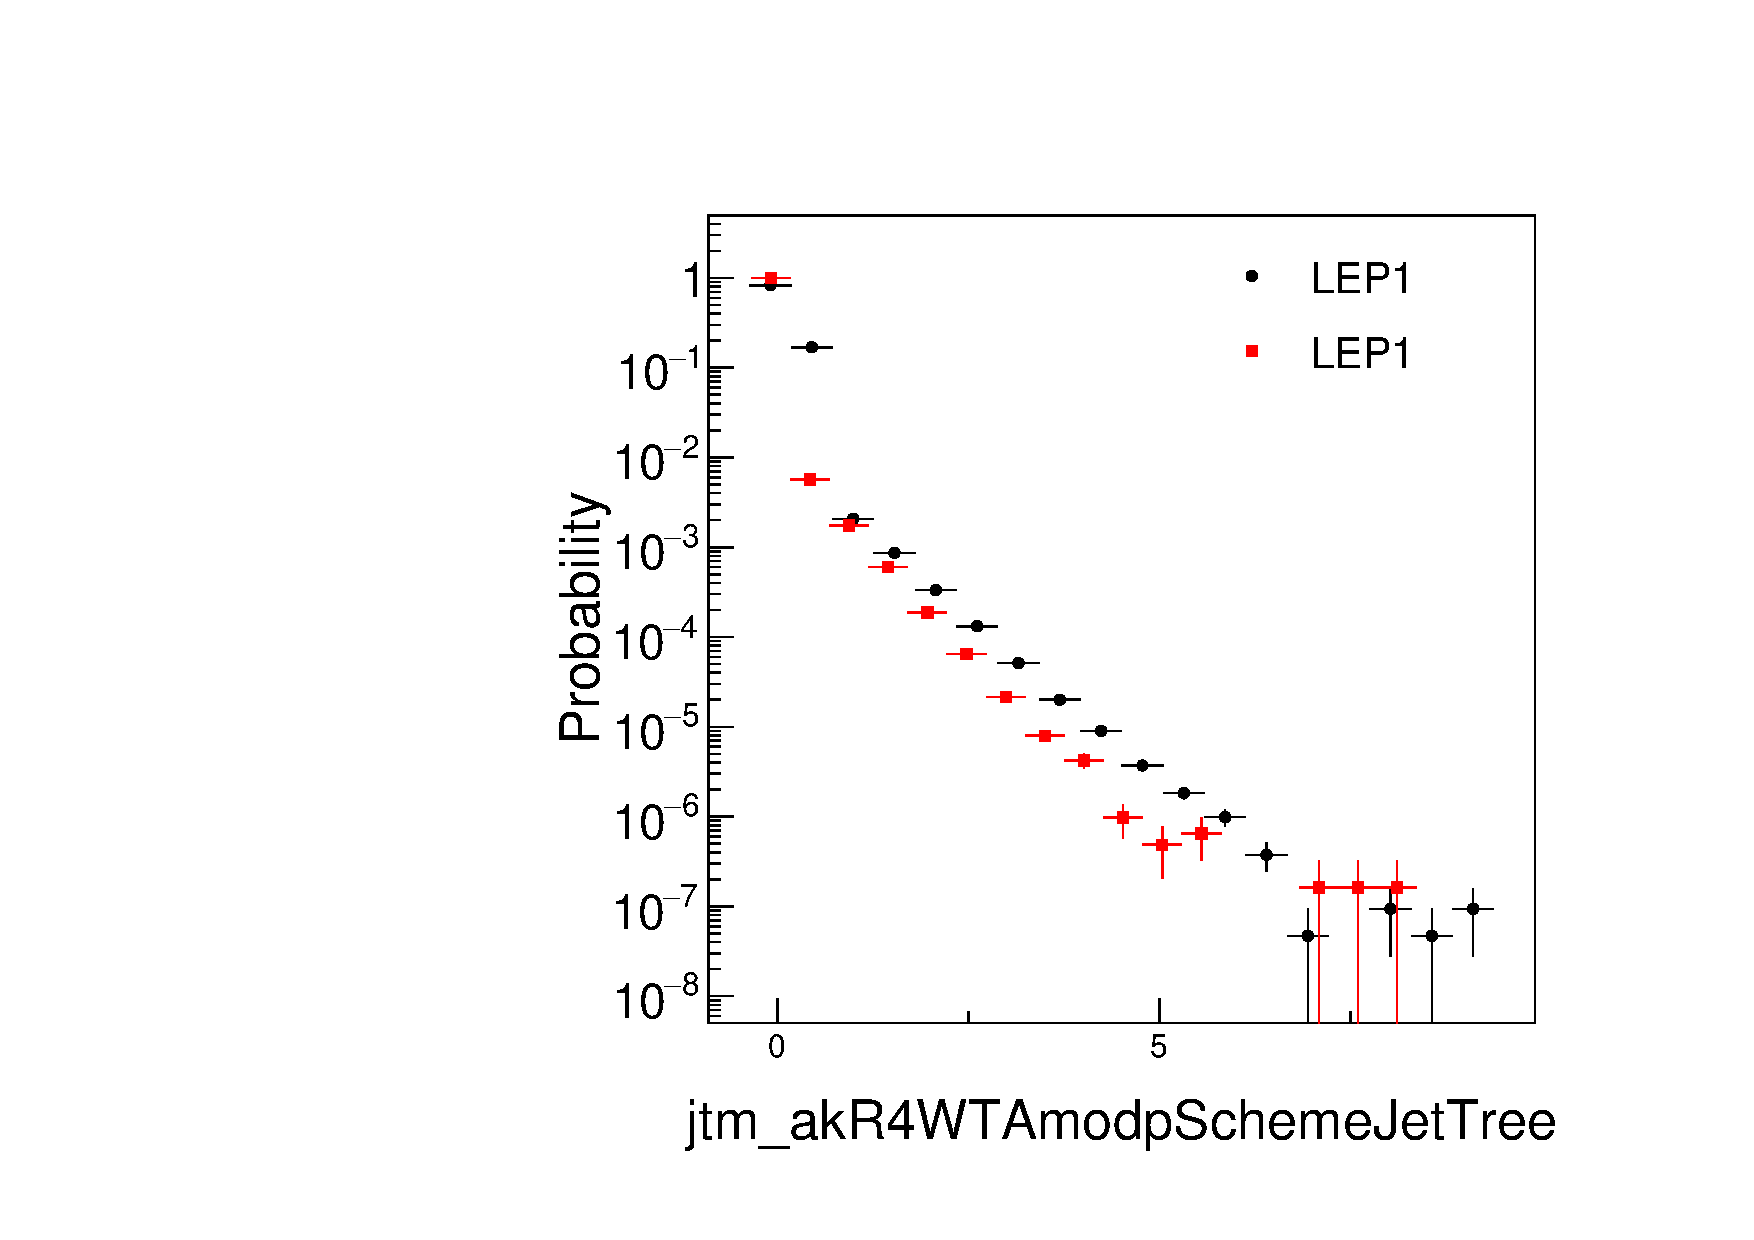
\includegraphics[width=.25\textwidth]{images/DQC/LEP1/jtm_akR4WTAmodpSchemeJetTree.pdf}}\hfill
\subfloat{\label{sfig:d}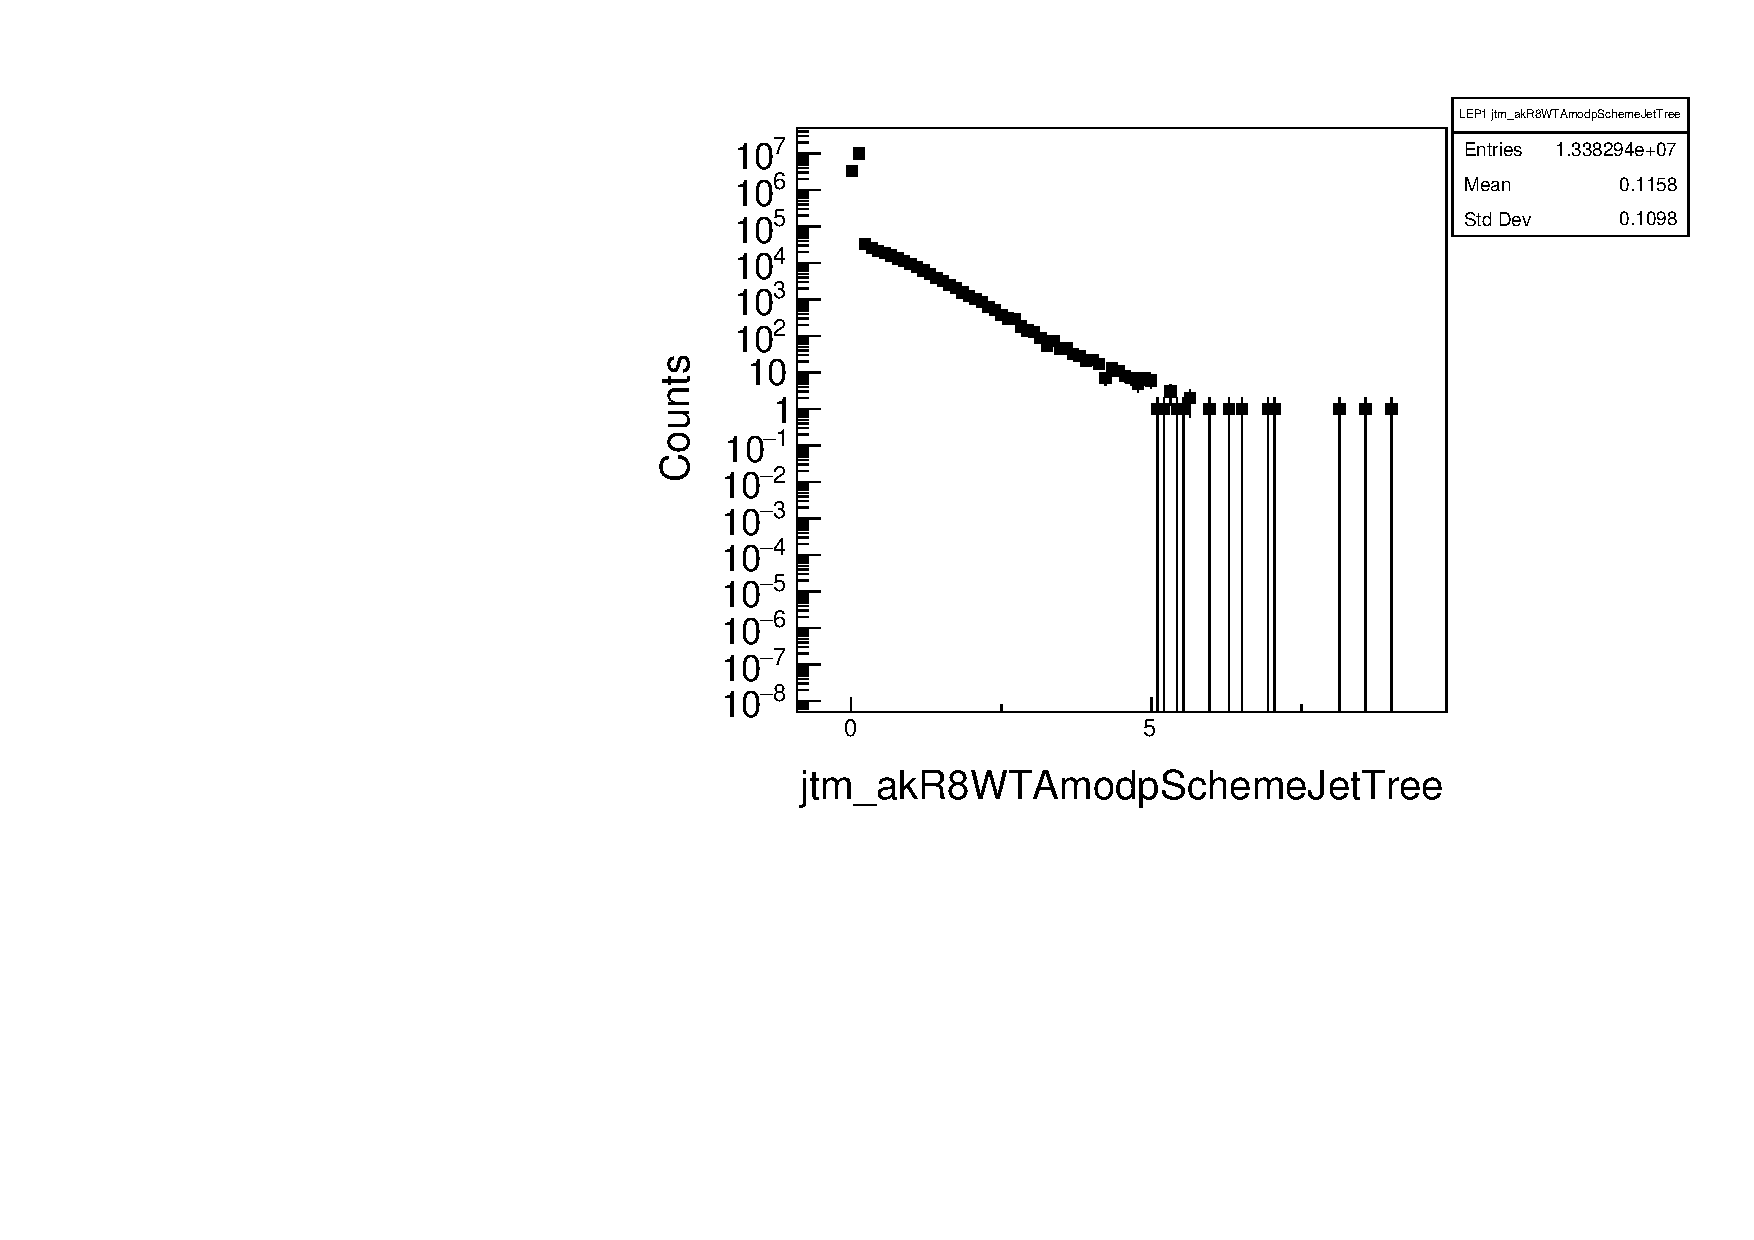
\includegraphics[width=.25\textwidth]{images/DQC/LEP1/jtm_akR8WTAmodpSchemeJetTree.pdf}}\hfill %row end
\subfloat{\label{sfig:e}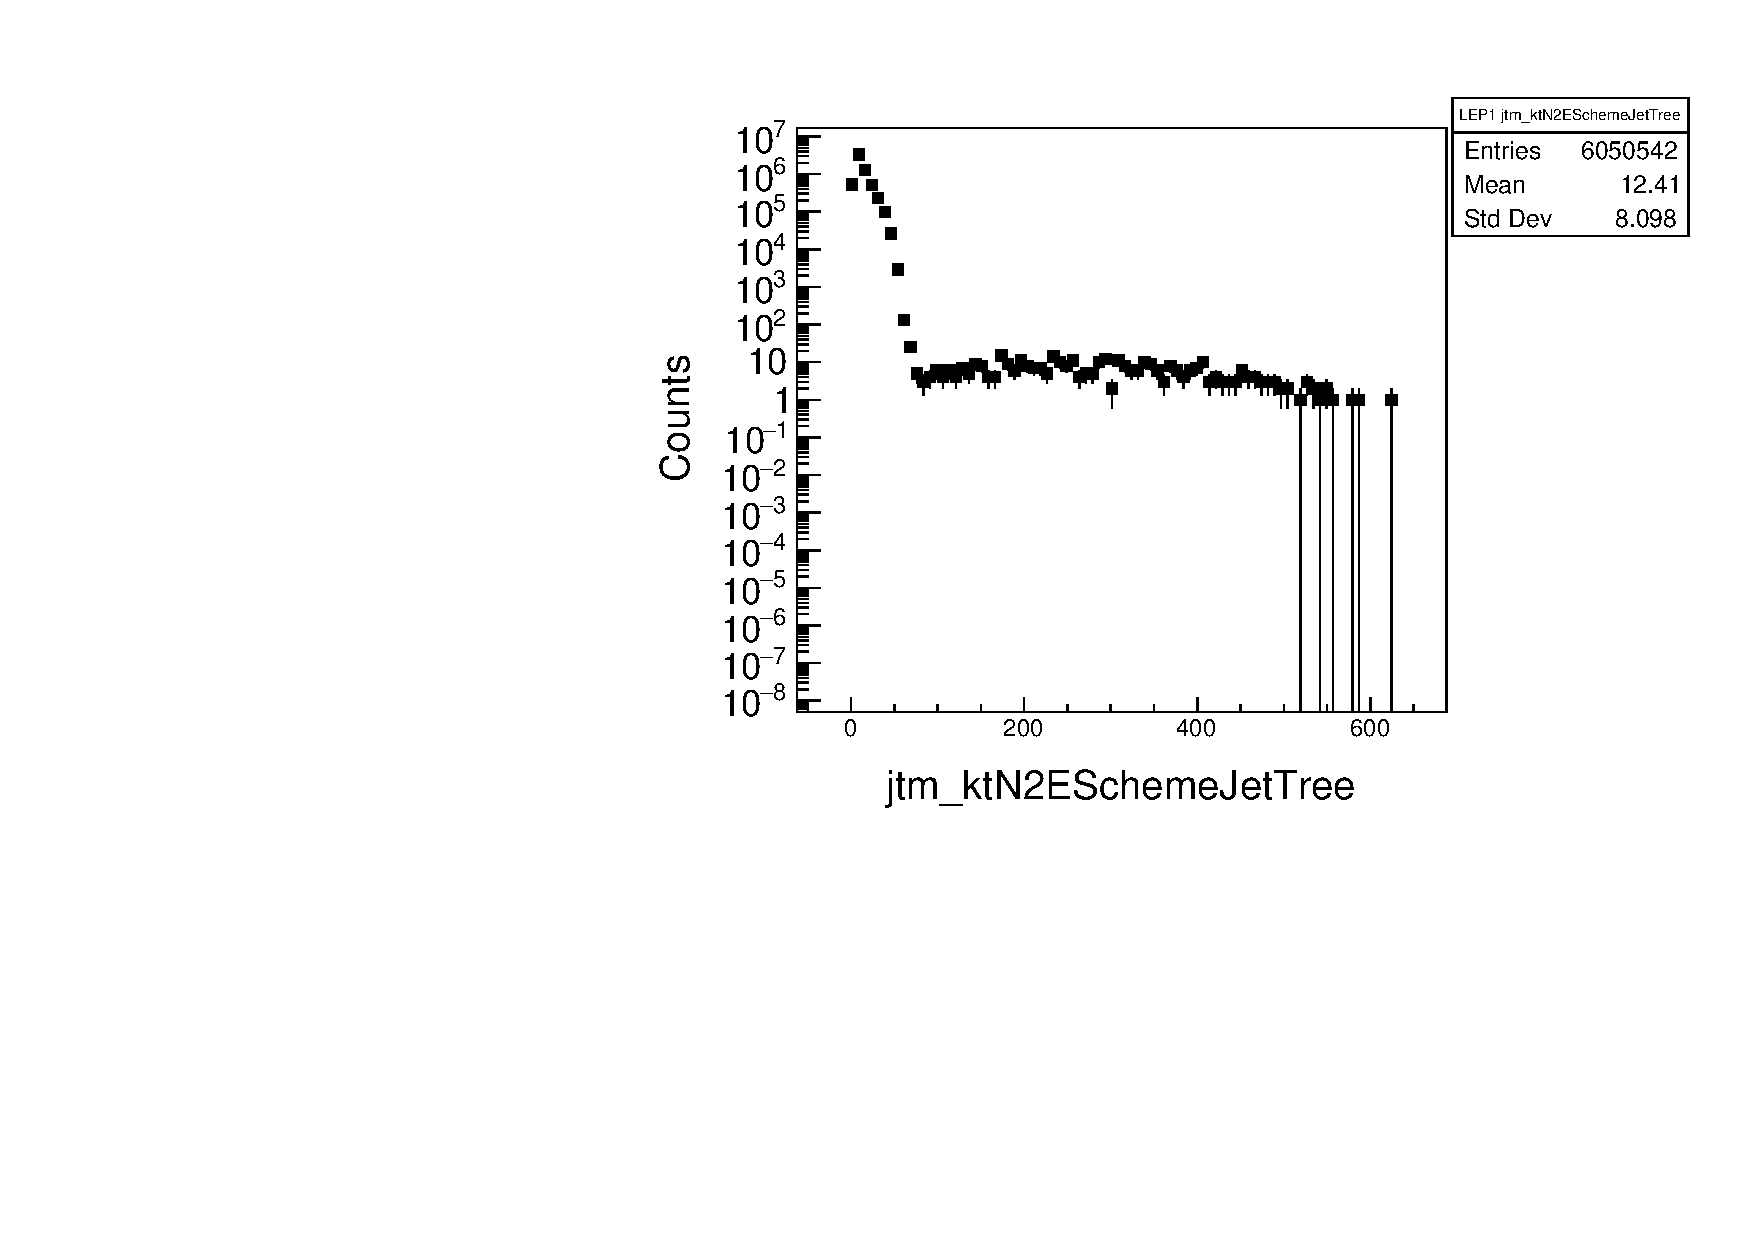
\includegraphics[width=.25\textwidth]{images/DQC/LEP1/jtm_ktN2ESchemeJetTree.pdf}}\hfill
\subfloat{\label{sfig:f}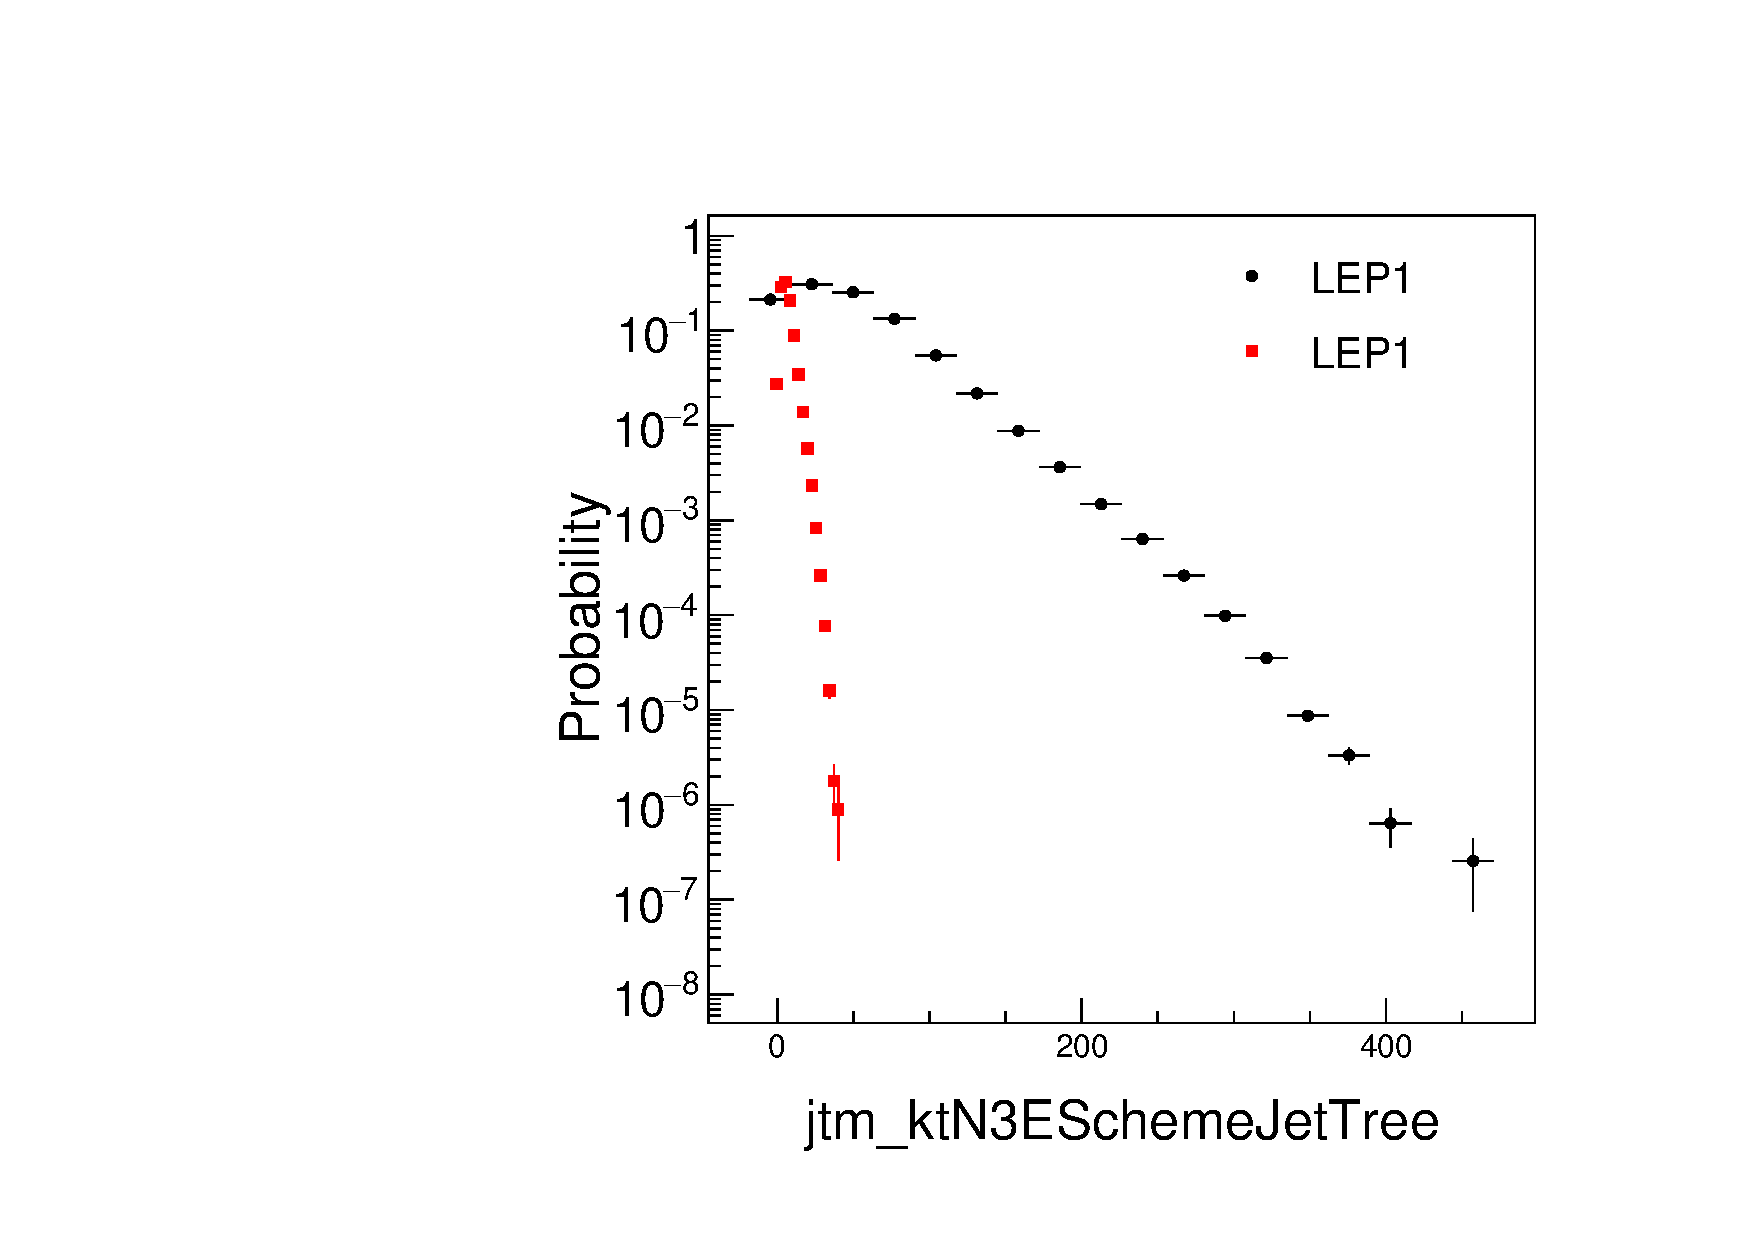
\includegraphics[width=.25\textwidth]{images/DQC/LEP1/jtm_ktN3ESchemeJetTree.pdf}}\hfill
\subfloat{\label{sfig:g}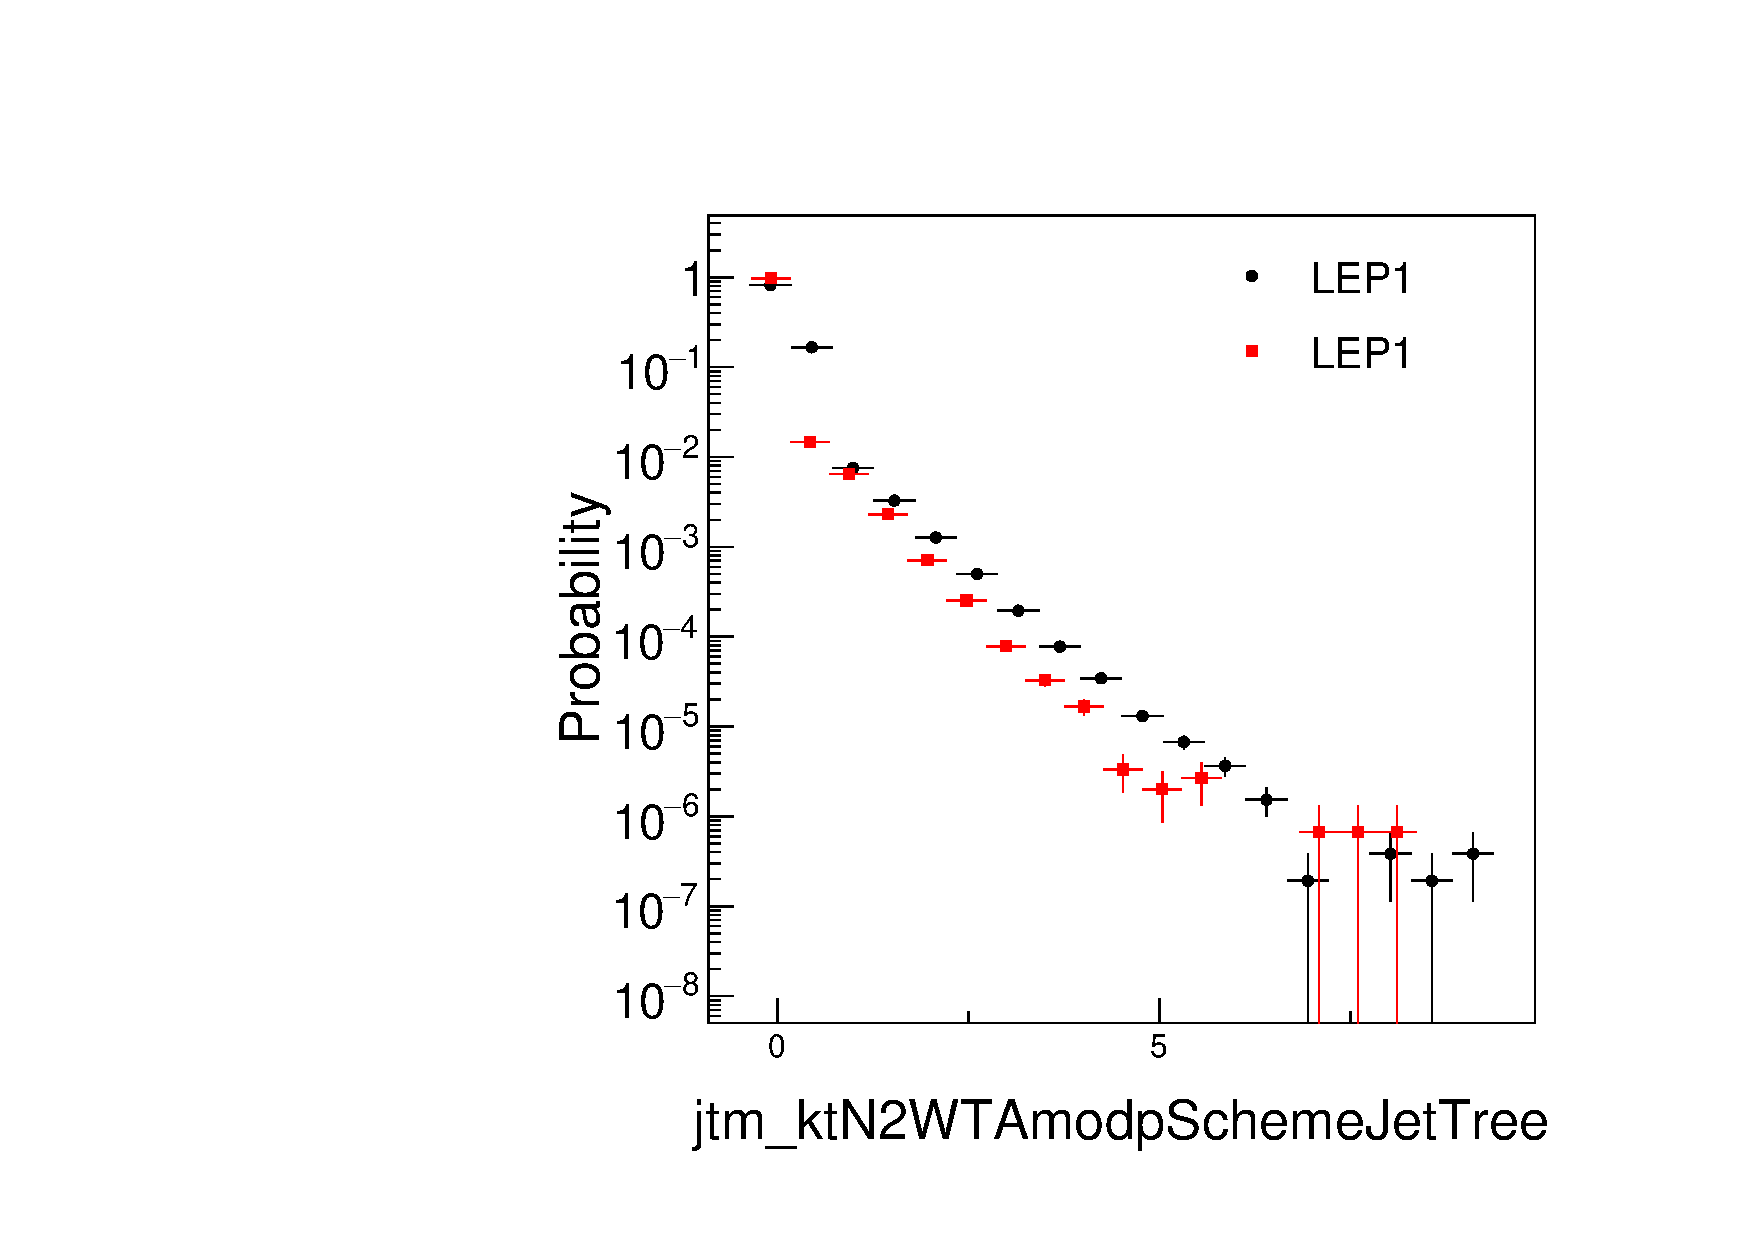
\includegraphics[width=.25\textwidth]{images/DQC/LEP1/jtm_ktN2WTAmodpSchemeJetTree.pdf}}\hfill
\subfloat{\label{sfig:h}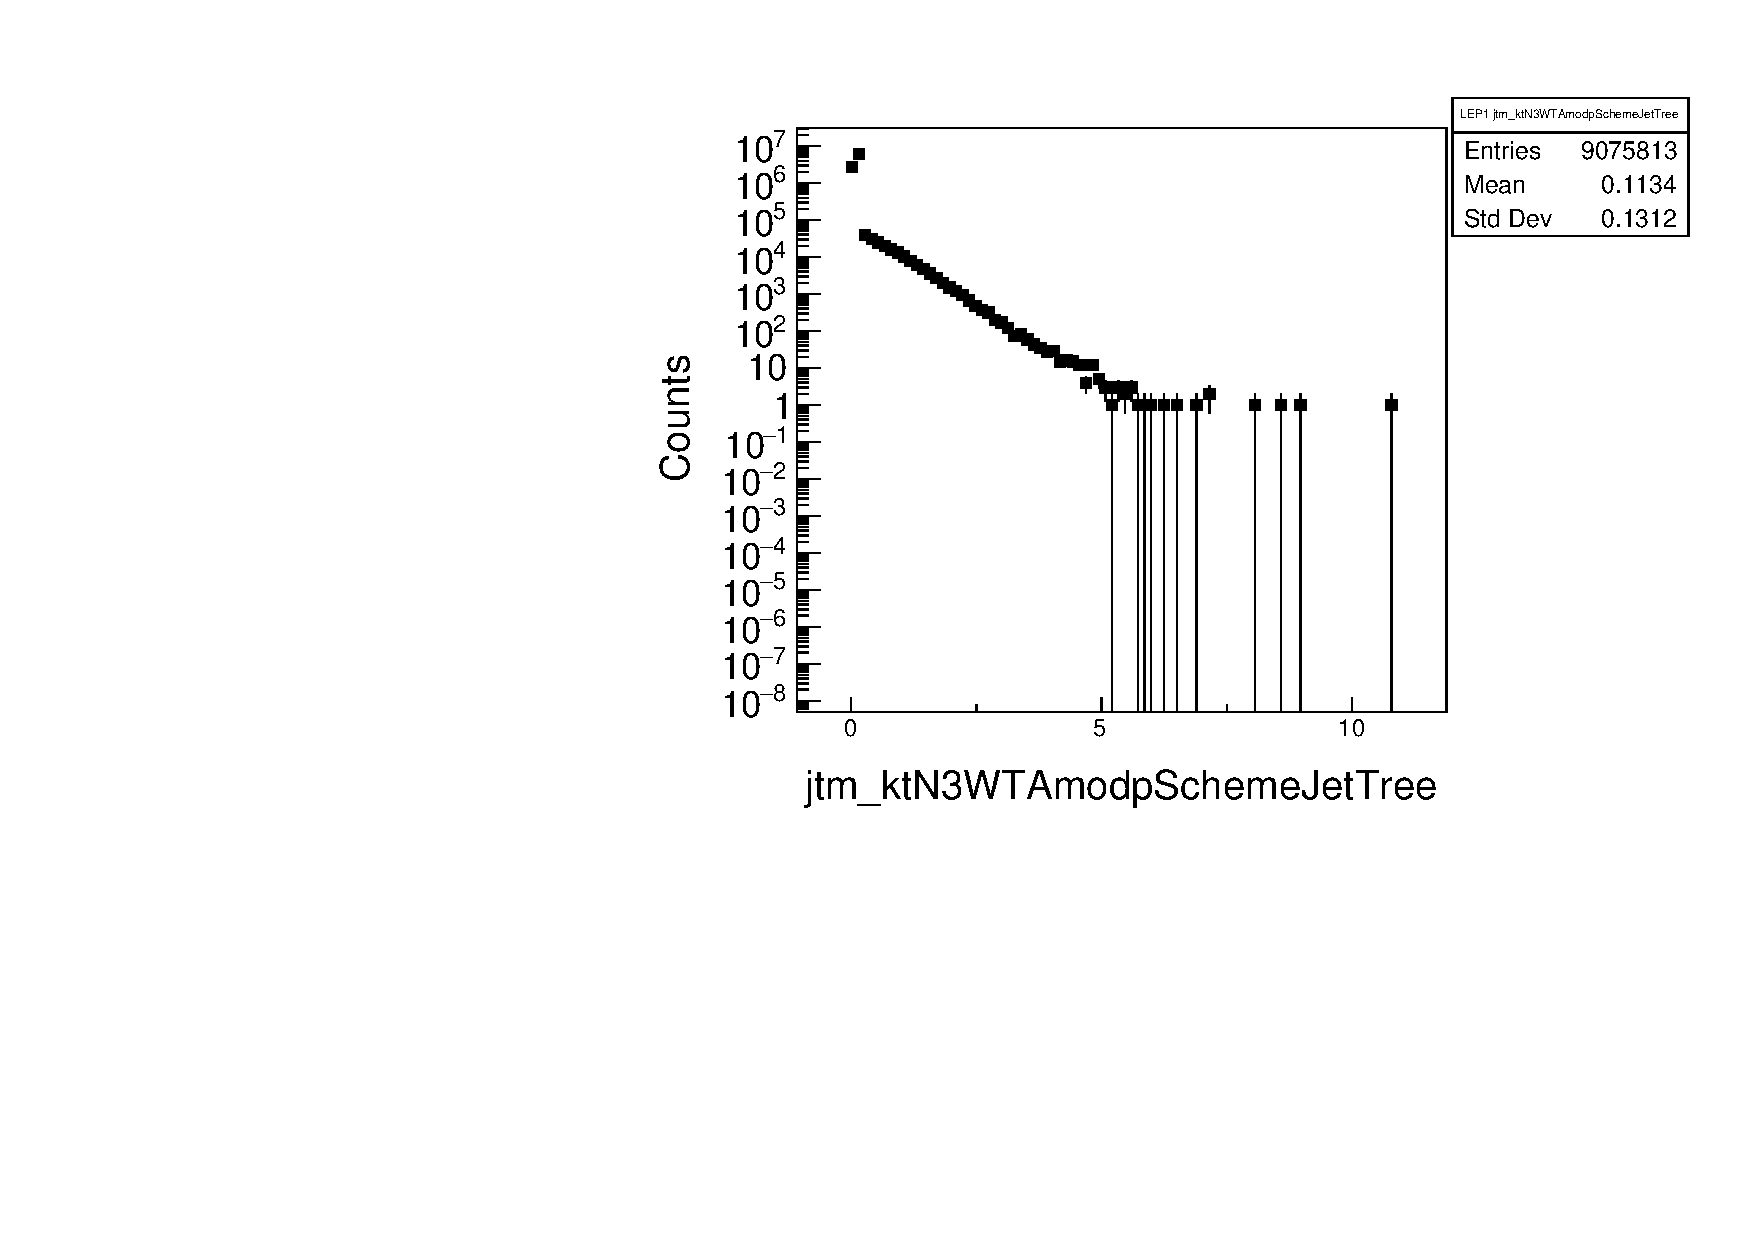
\includegraphics[width=.25\textwidth]{images/DQC/LEP1/jtm_ktN3WTAmodpSchemeJetTree.pdf}}\hfill
\caption{LEP1 Jet mass distributions. Top row: anti-$k_t$, left to right: $R=0.4$, $E$ scheme; $R=0.8$, $E$ scheme; $R=0.4$, WTA mod p scheme; $R=0.8$, WTA mod p scheme. Bottom row: $k_t$, left to right: $N=2$, $E$ scheme; $N=3$, $E$ scheme; $N=2$, WTA mod p scheme; $N=3$; WTA mod p scheme.}  
\end{figure}

\begin{figure}[H]
\centering
\subfloat{\label{sfig:a}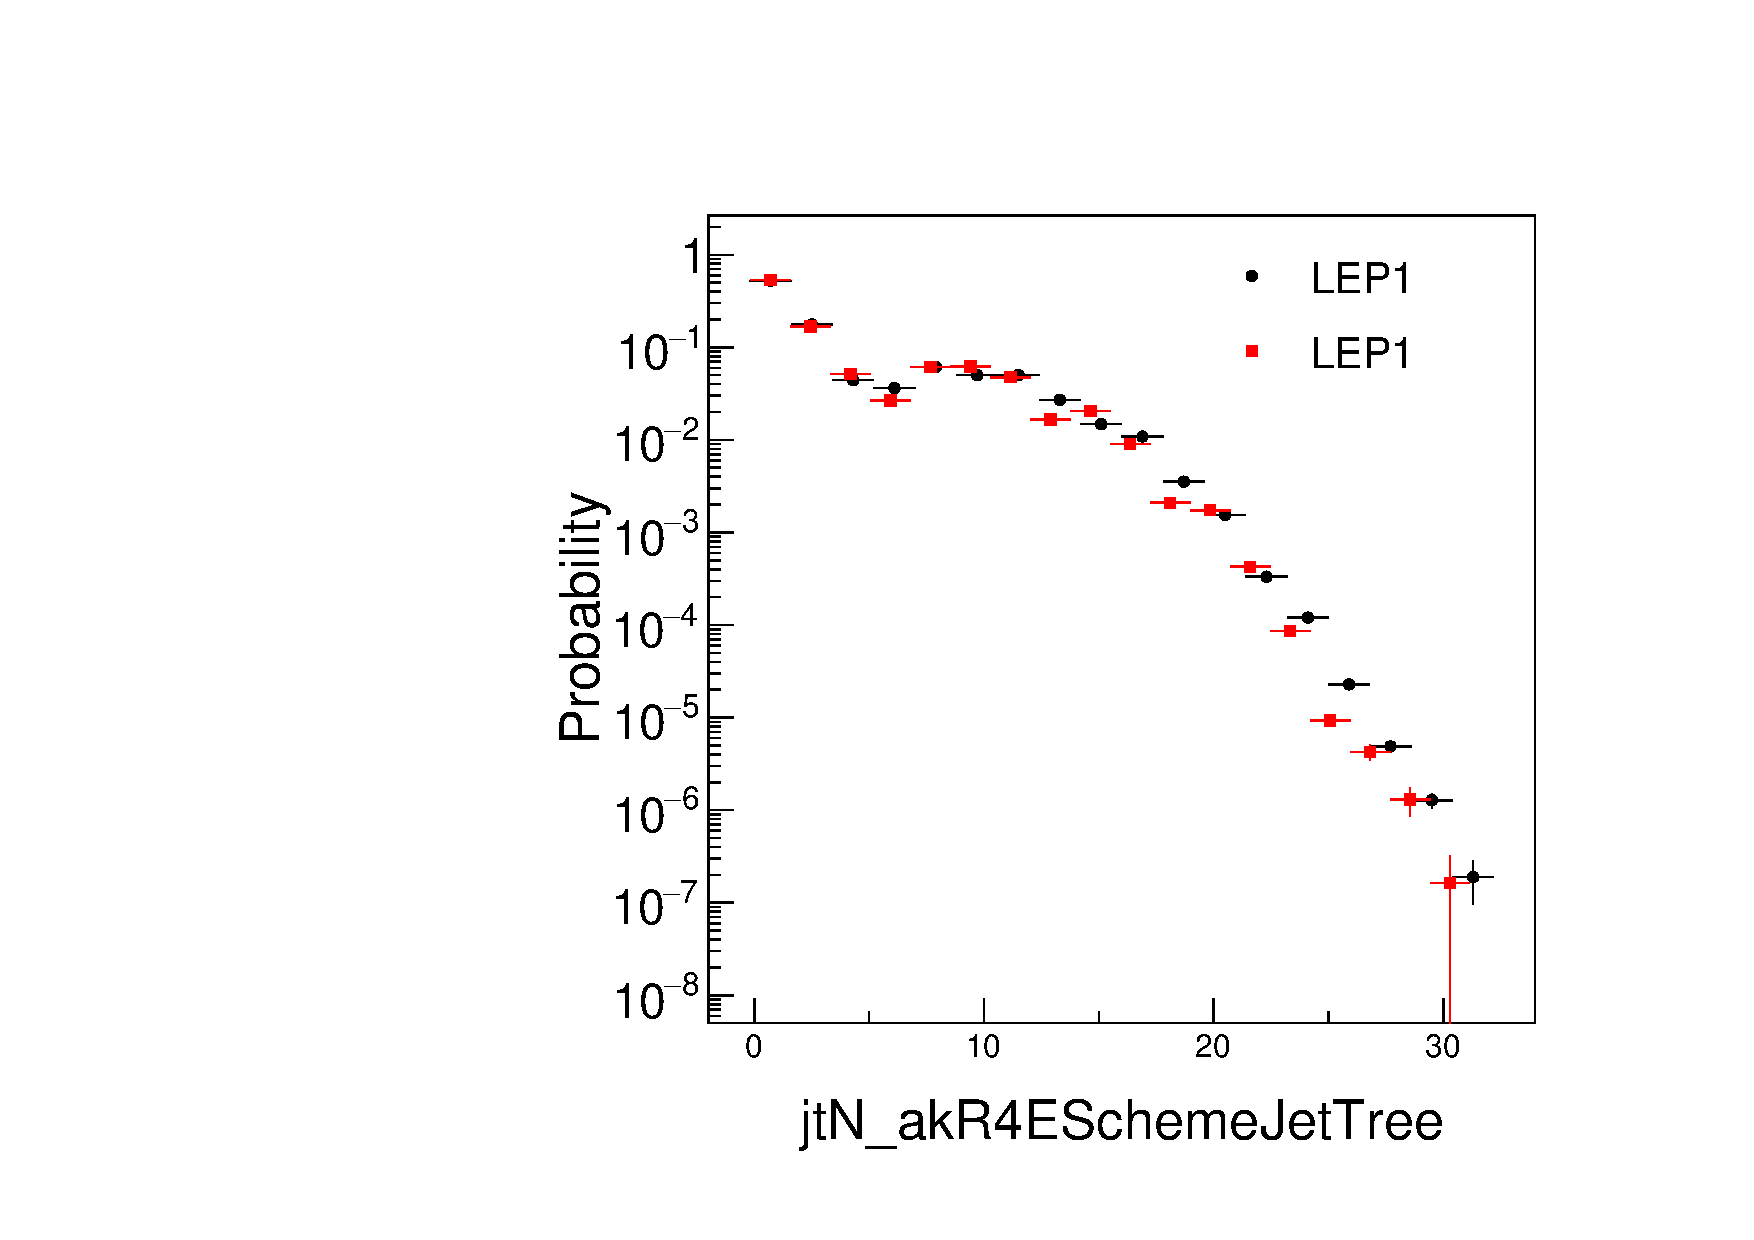
\includegraphics[width=.25\textwidth]{images/DQC/LEP1/jtN_akR4ESchemeJetTree.pdf}}\hfill
\subfloat{\label{sfig:b}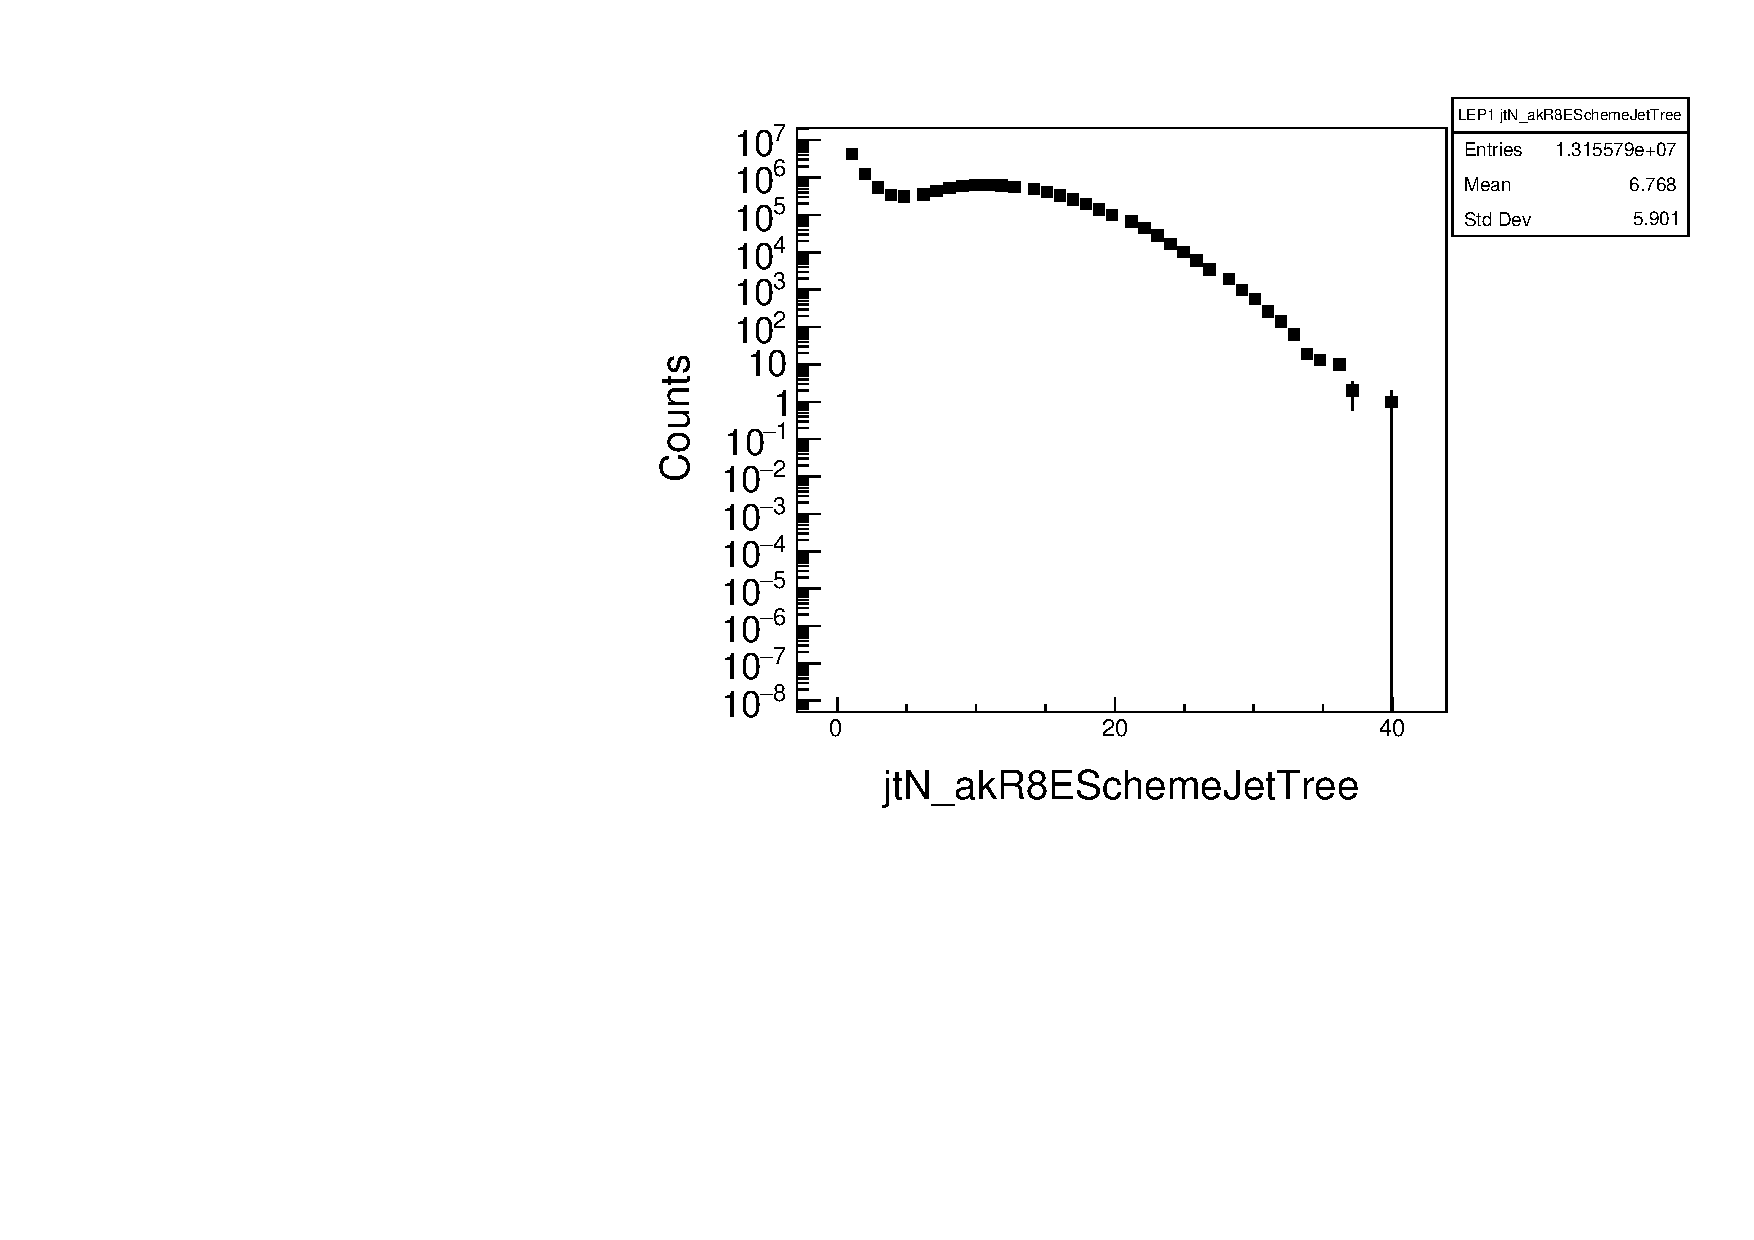
\includegraphics[width=.25\textwidth]{images/DQC/LEP1/jtN_akR8ESchemeJetTree.pdf}}\hfill
\subfloat{\label{sfig:c}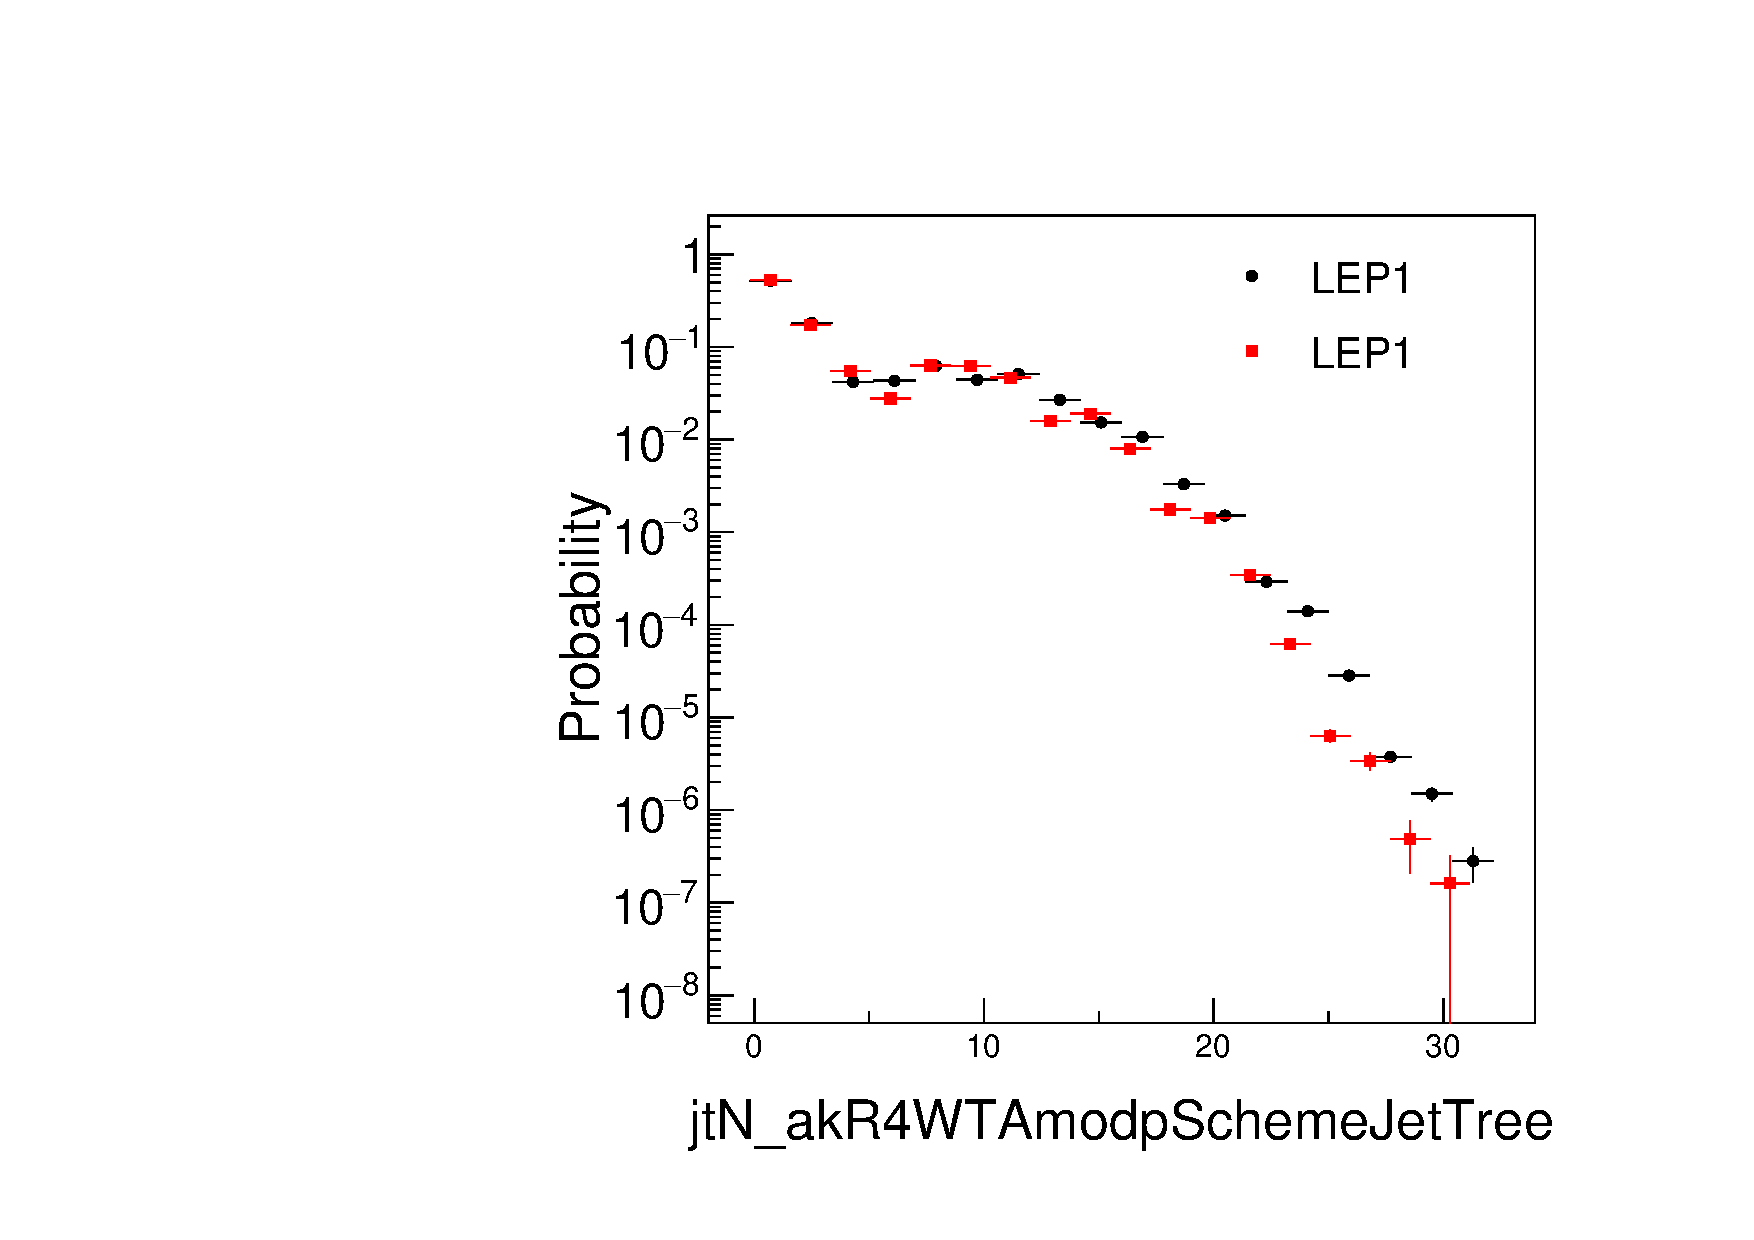
\includegraphics[width=.25\textwidth]{images/DQC/LEP1/jtN_akR4WTAmodpSchemeJetTree.pdf}}\hfill
\subfloat{\label{sfig:d}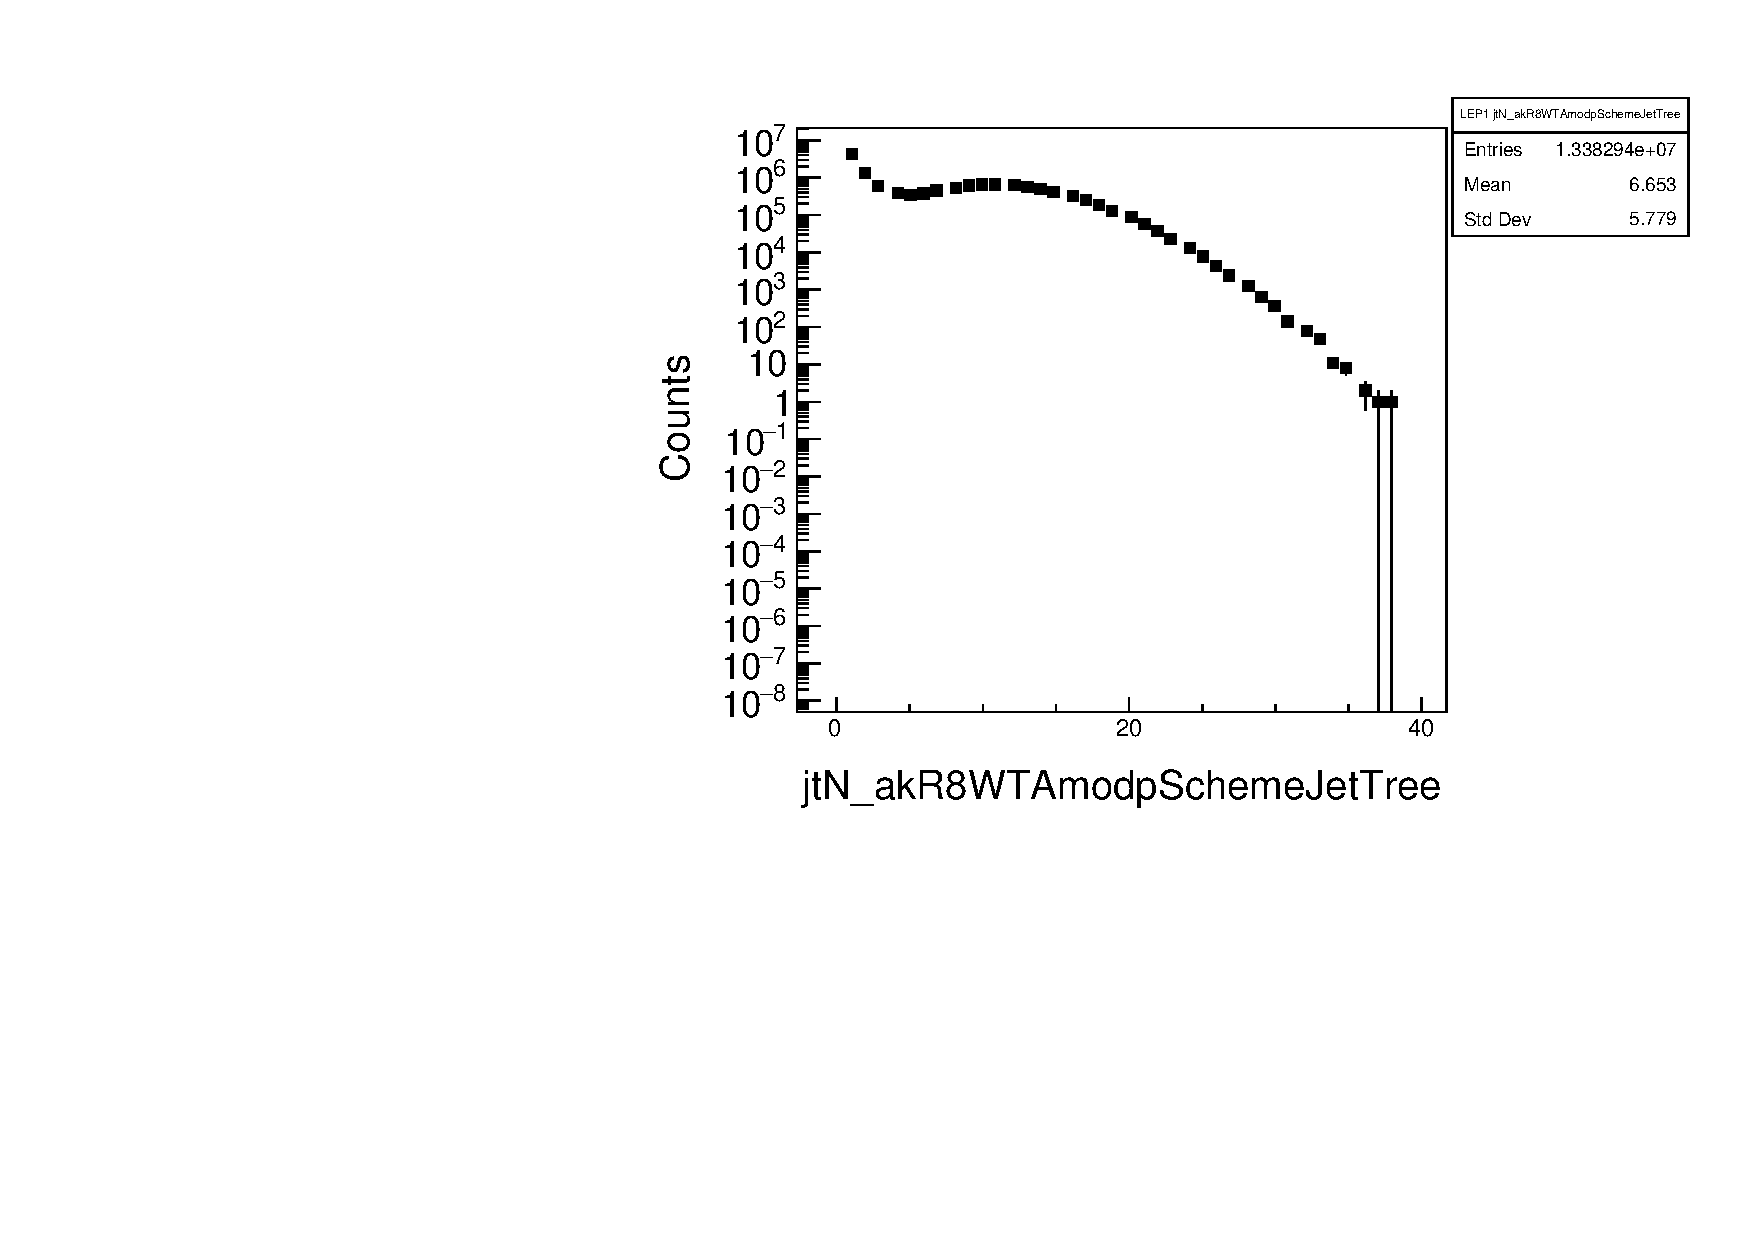
\includegraphics[width=.25\textwidth]{images/DQC/LEP1/jtN_akR8WTAmodpSchemeJetTree.pdf}}\hfill %row end
\subfloat{\label{sfig:e}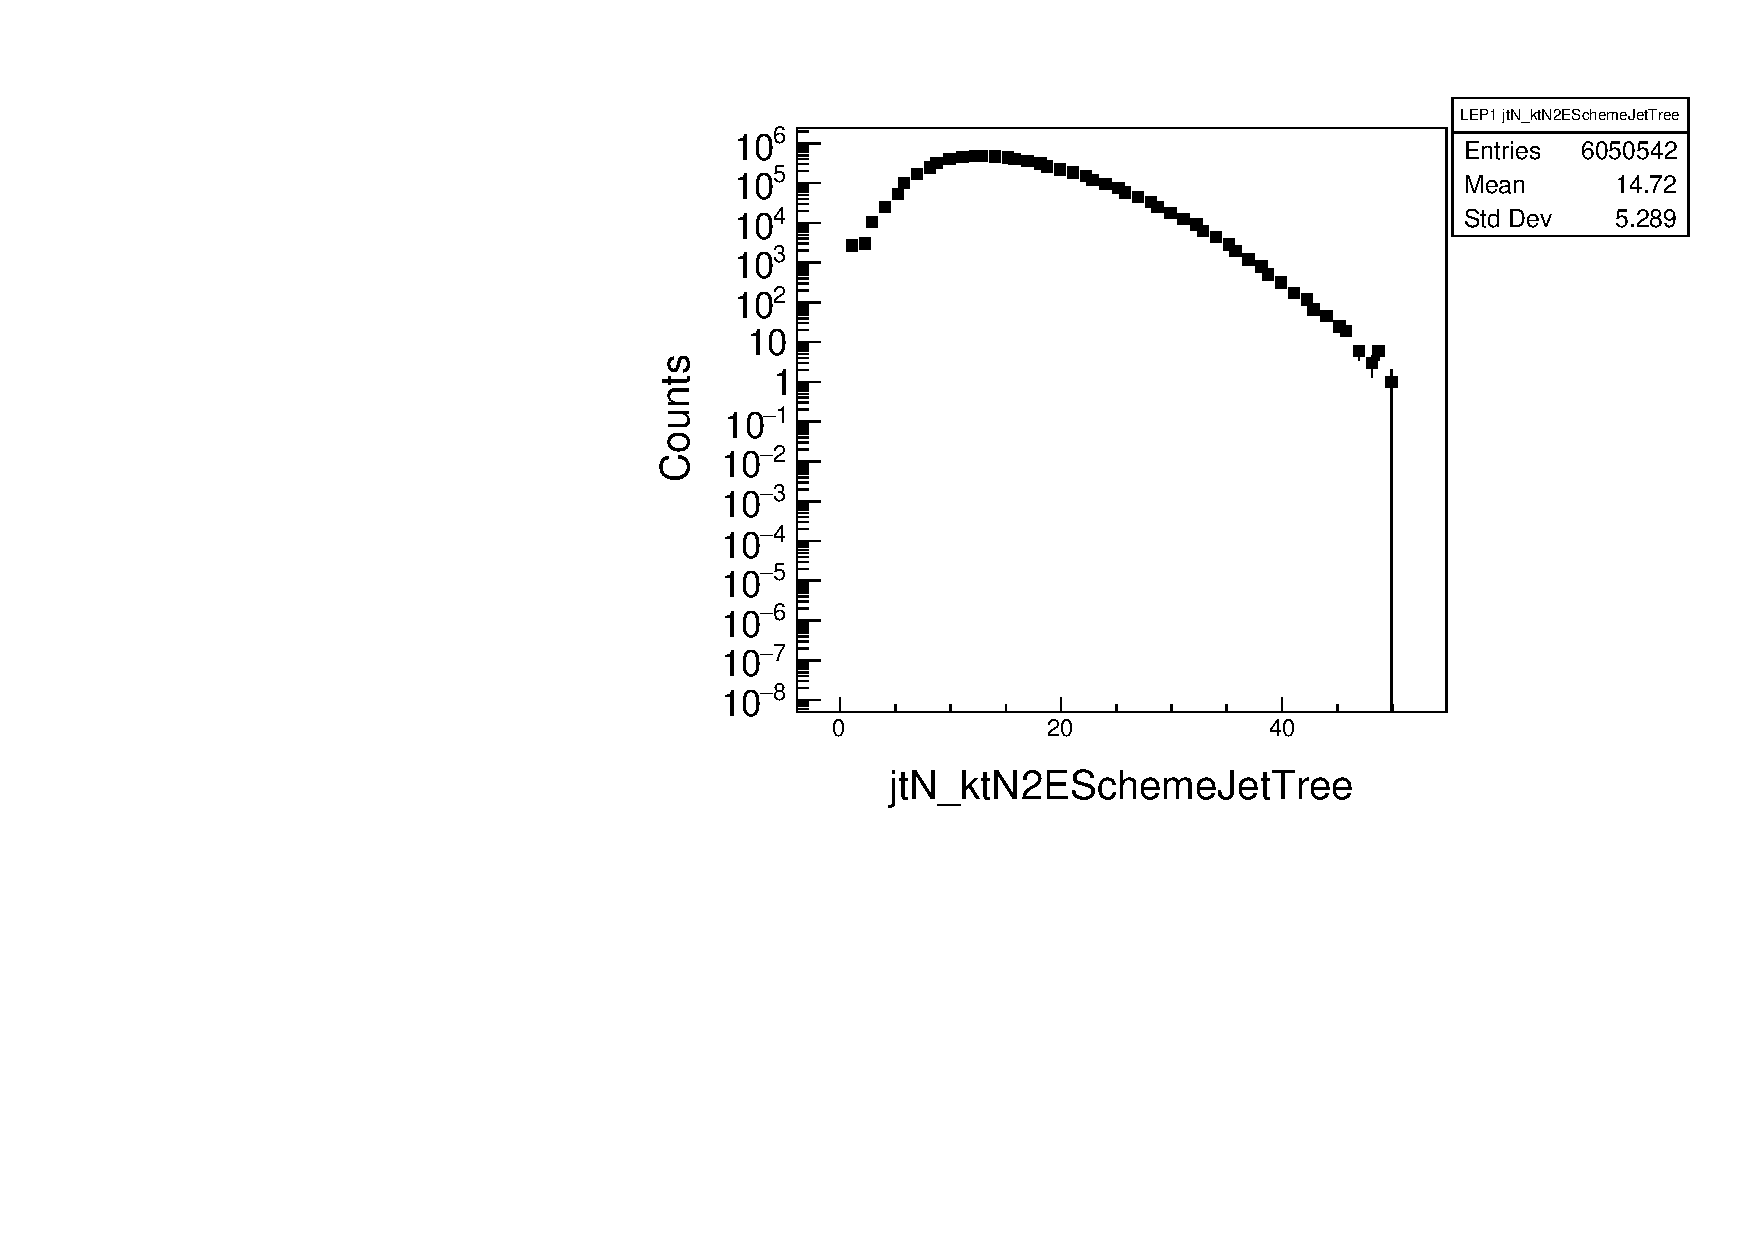
\includegraphics[width=.25\textwidth]{images/DQC/LEP1/jtN_ktN2ESchemeJetTree.pdf}}\hfill
\subfloat{\label{sfig:f}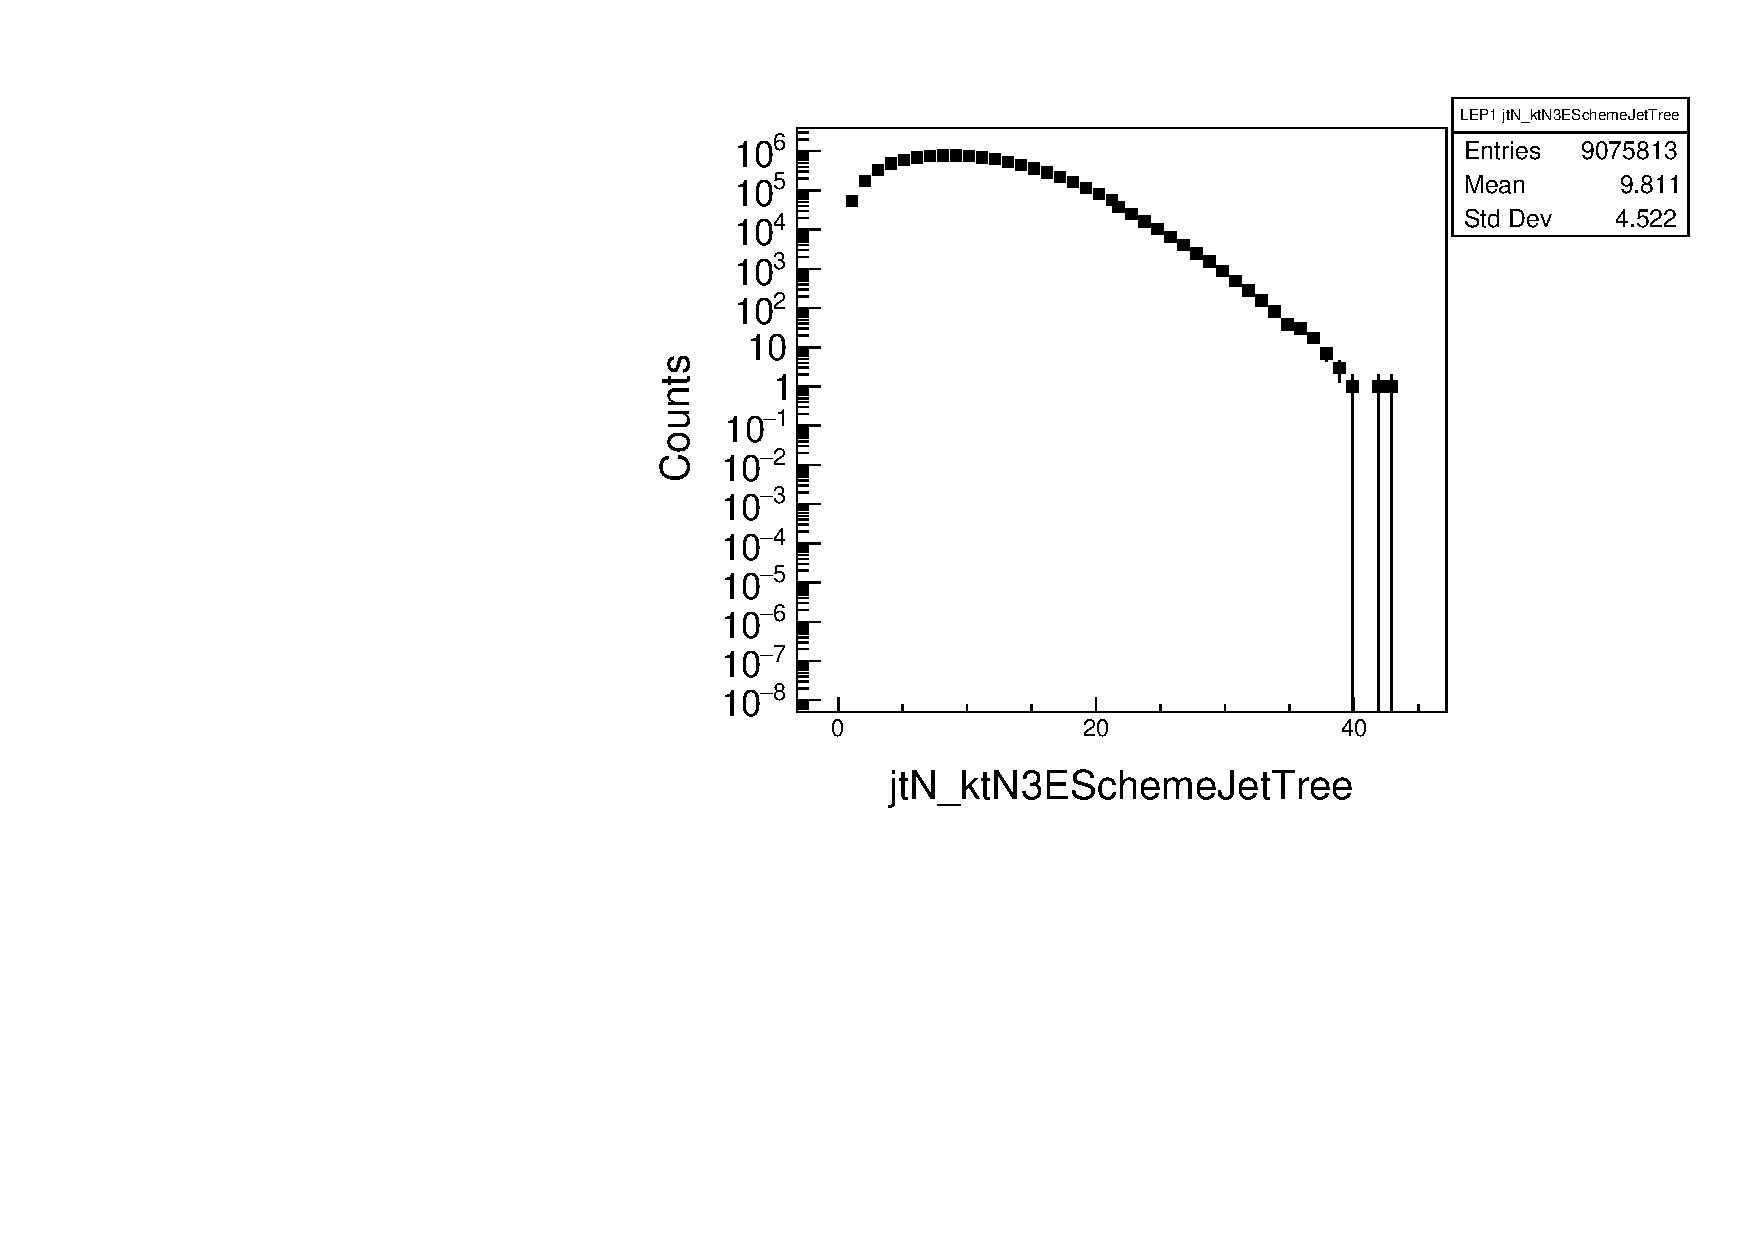
\includegraphics[width=.25\textwidth]{images/DQC/LEP1/jtN_ktN3ESchemeJetTree.pdf}}\hfill
\subfloat{\label{sfig:g}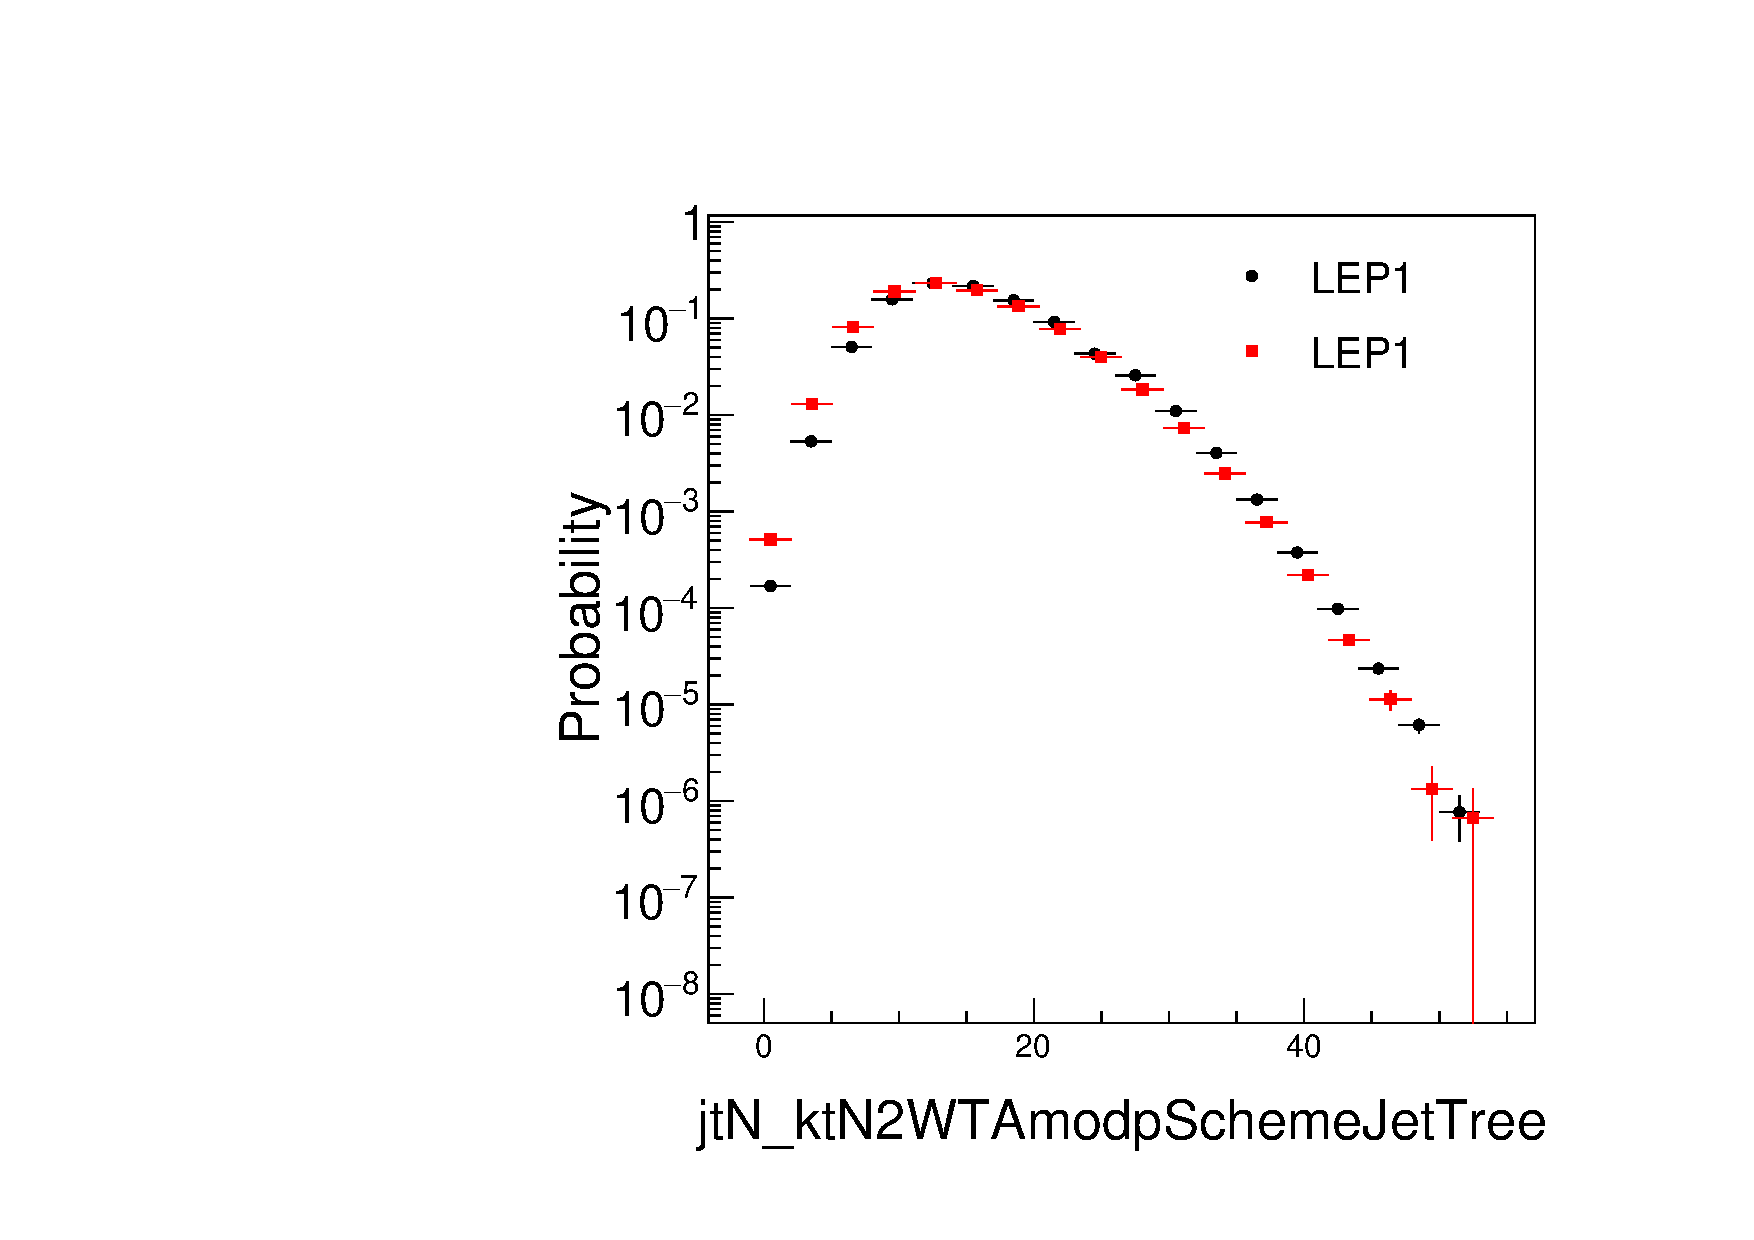
\includegraphics[width=.25\textwidth]{images/DQC/LEP1/jtN_ktN2WTAmodpSchemeJetTree.pdf}}\hfill
\subfloat{\label{sfig:h}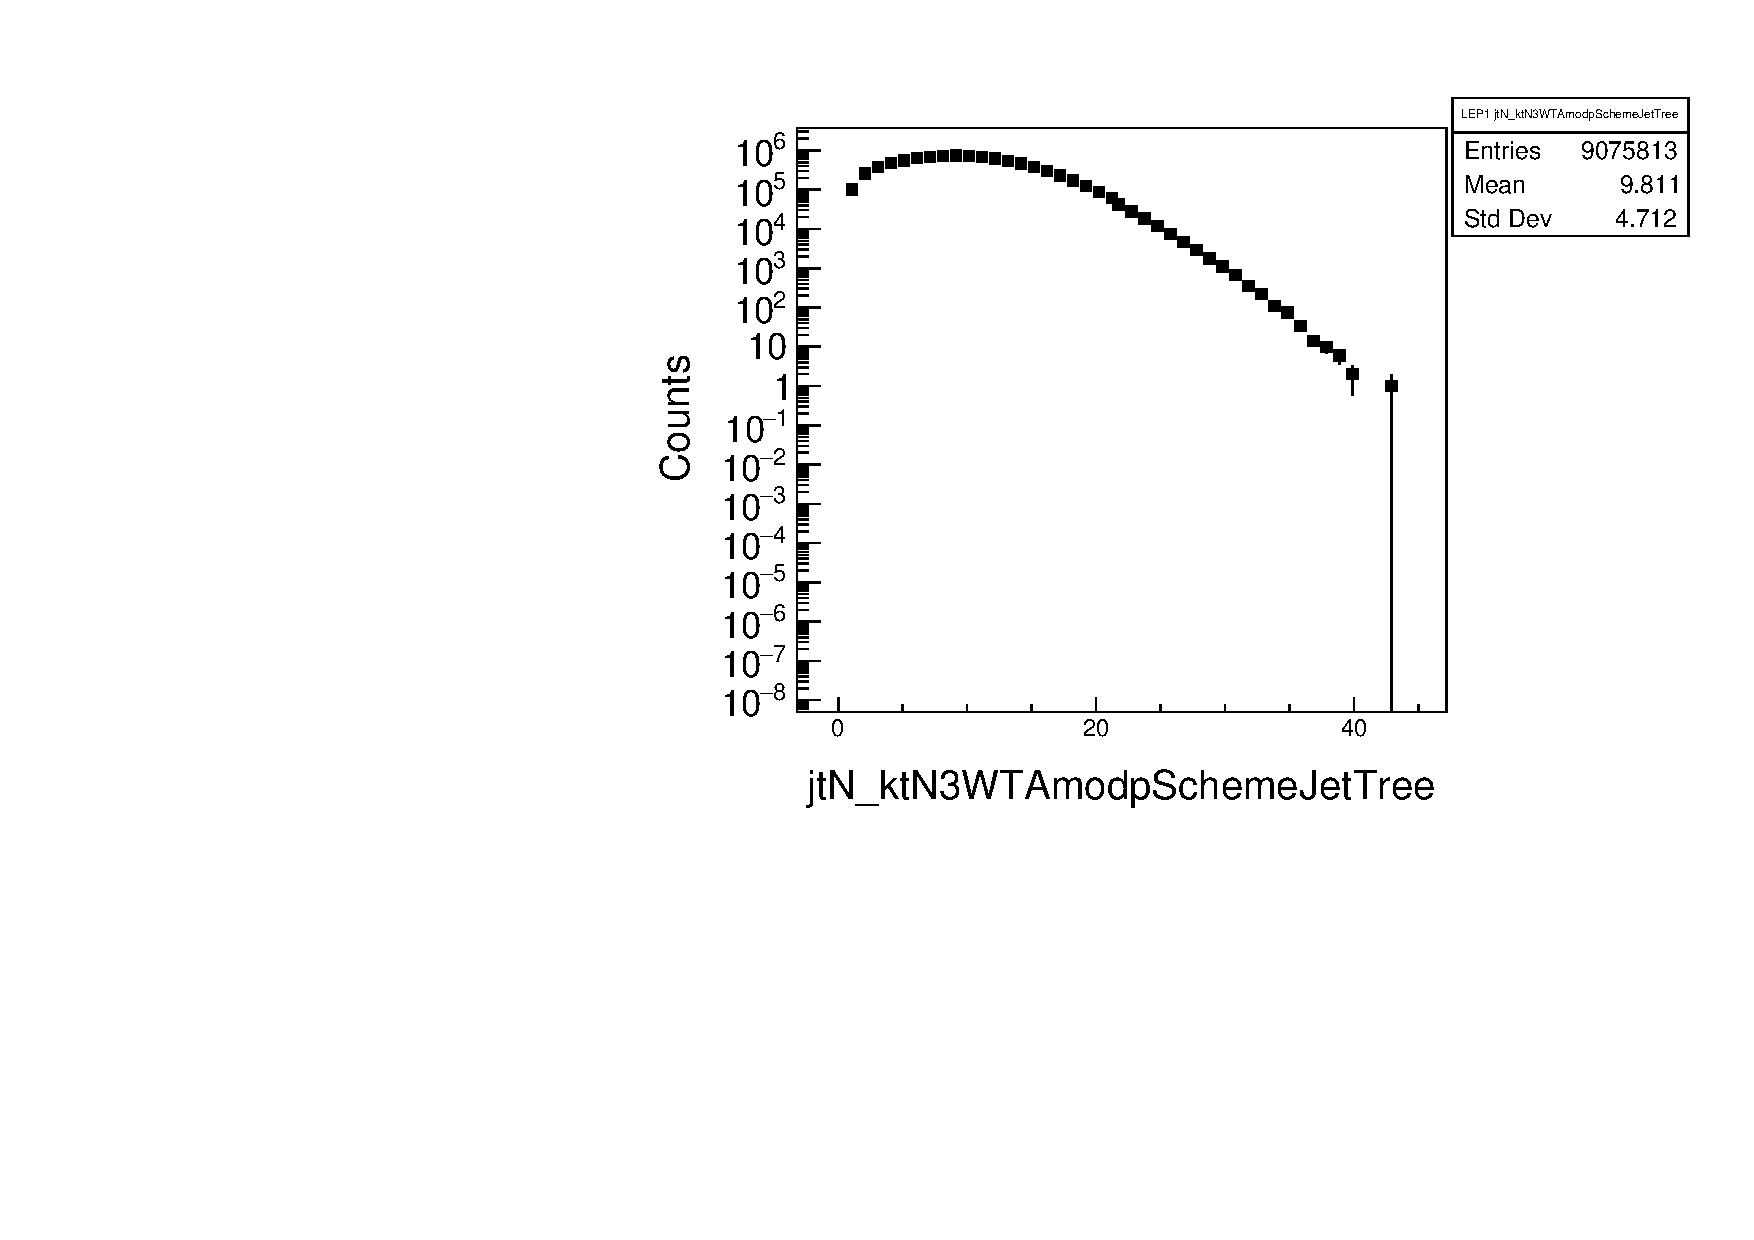
\includegraphics[width=.25\textwidth]{images/DQC/LEP1/jtN_ktN3WTAmodpSchemeJetTree.pdf}}\hfill
\caption{LEP1 Jet $N$ distributions. Top row: anti-$k_t$, left to right: $R=0.4$, $E$ scheme; $R=0.8$, $E$ scheme; $R=0.4$, WTA mod p scheme; $R=0.8$, WTA mod p scheme. Bottom row: $k_t$, left to right: $N=2$, $E$ scheme; $N=3$, $E$ scheme; $N=2$, WTA mod p scheme; $N=3$; WTA mod p scheme.}  
\end{figure} 

\begin{figure}[H]
\centering
\subfloat{\label{sfig:a}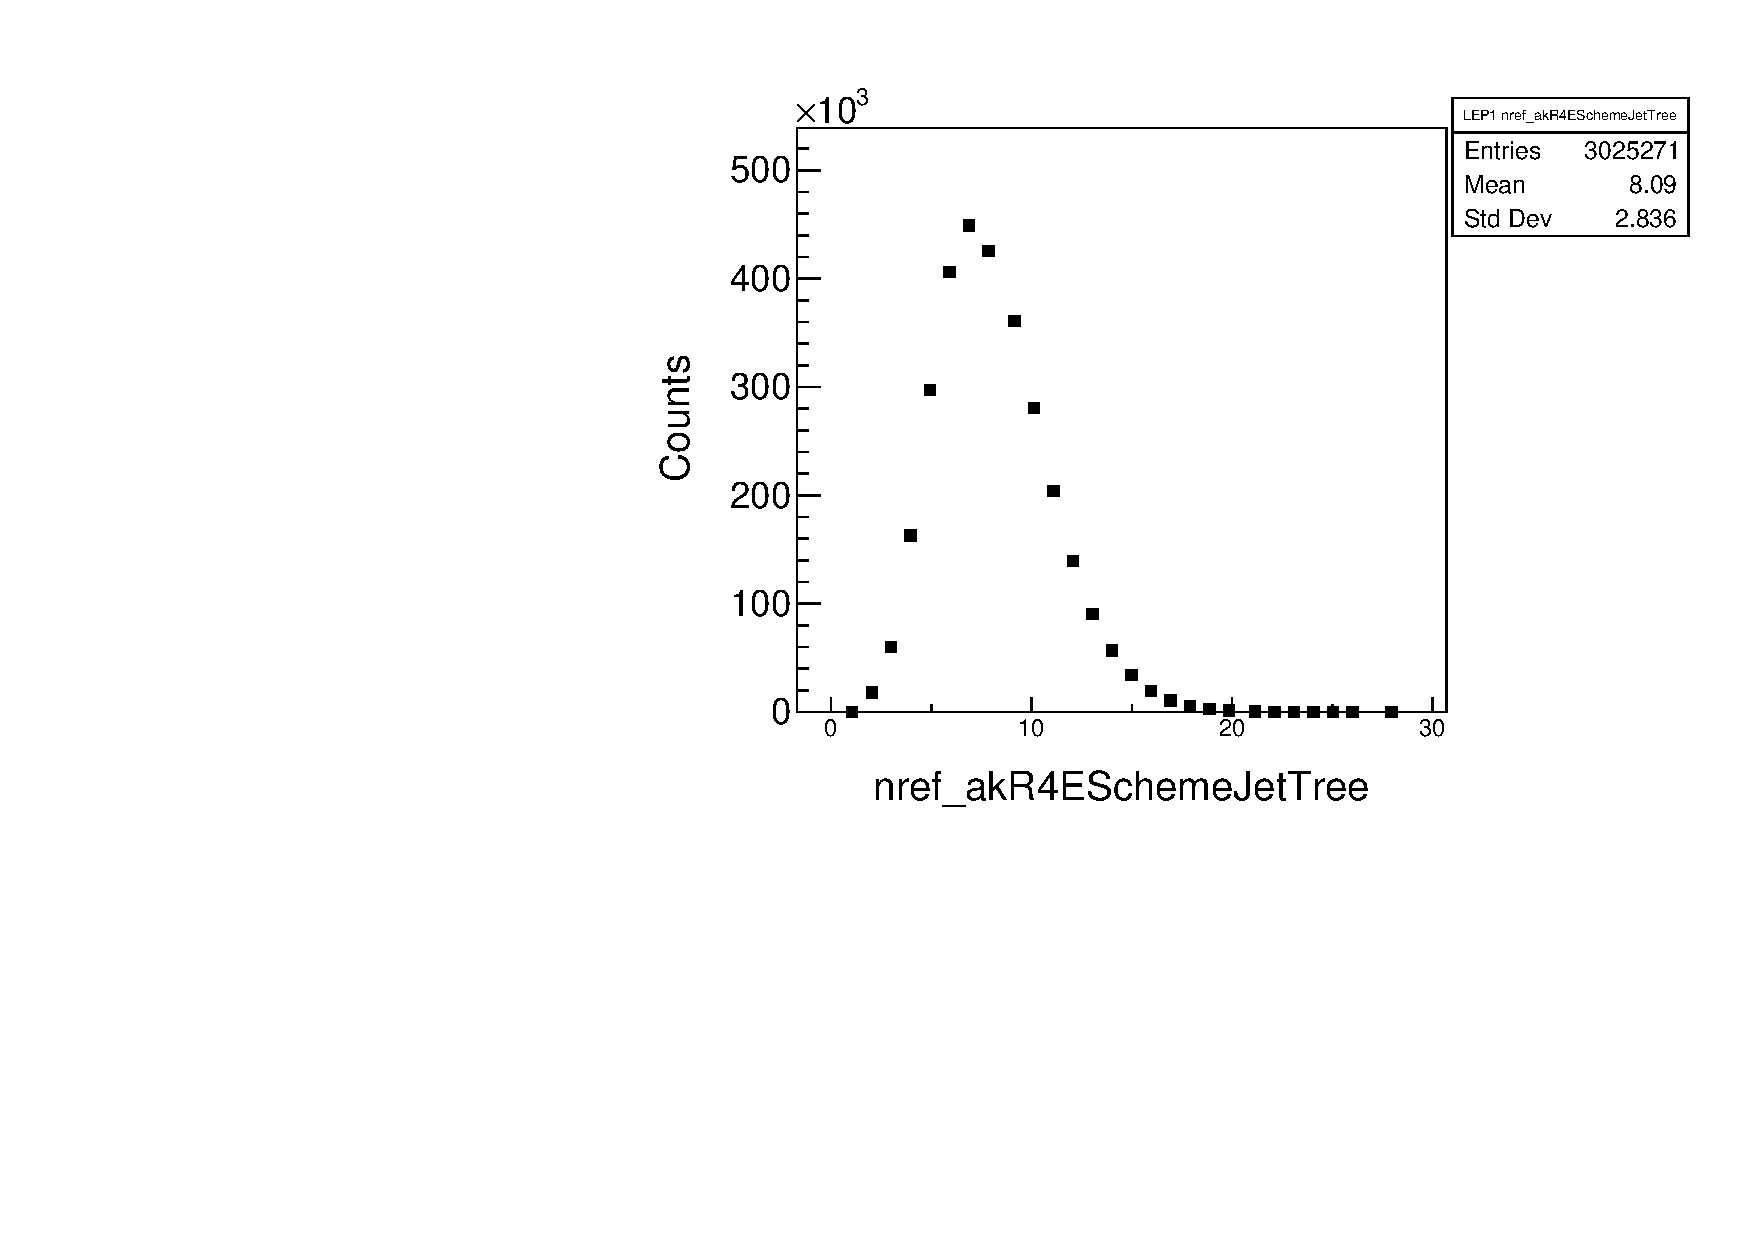
\includegraphics[width=.25\textwidth]{images/DQC/LEP1/nref_akR4ESchemeJetTree.pdf}}\hfill
\subfloat{\label{sfig:b}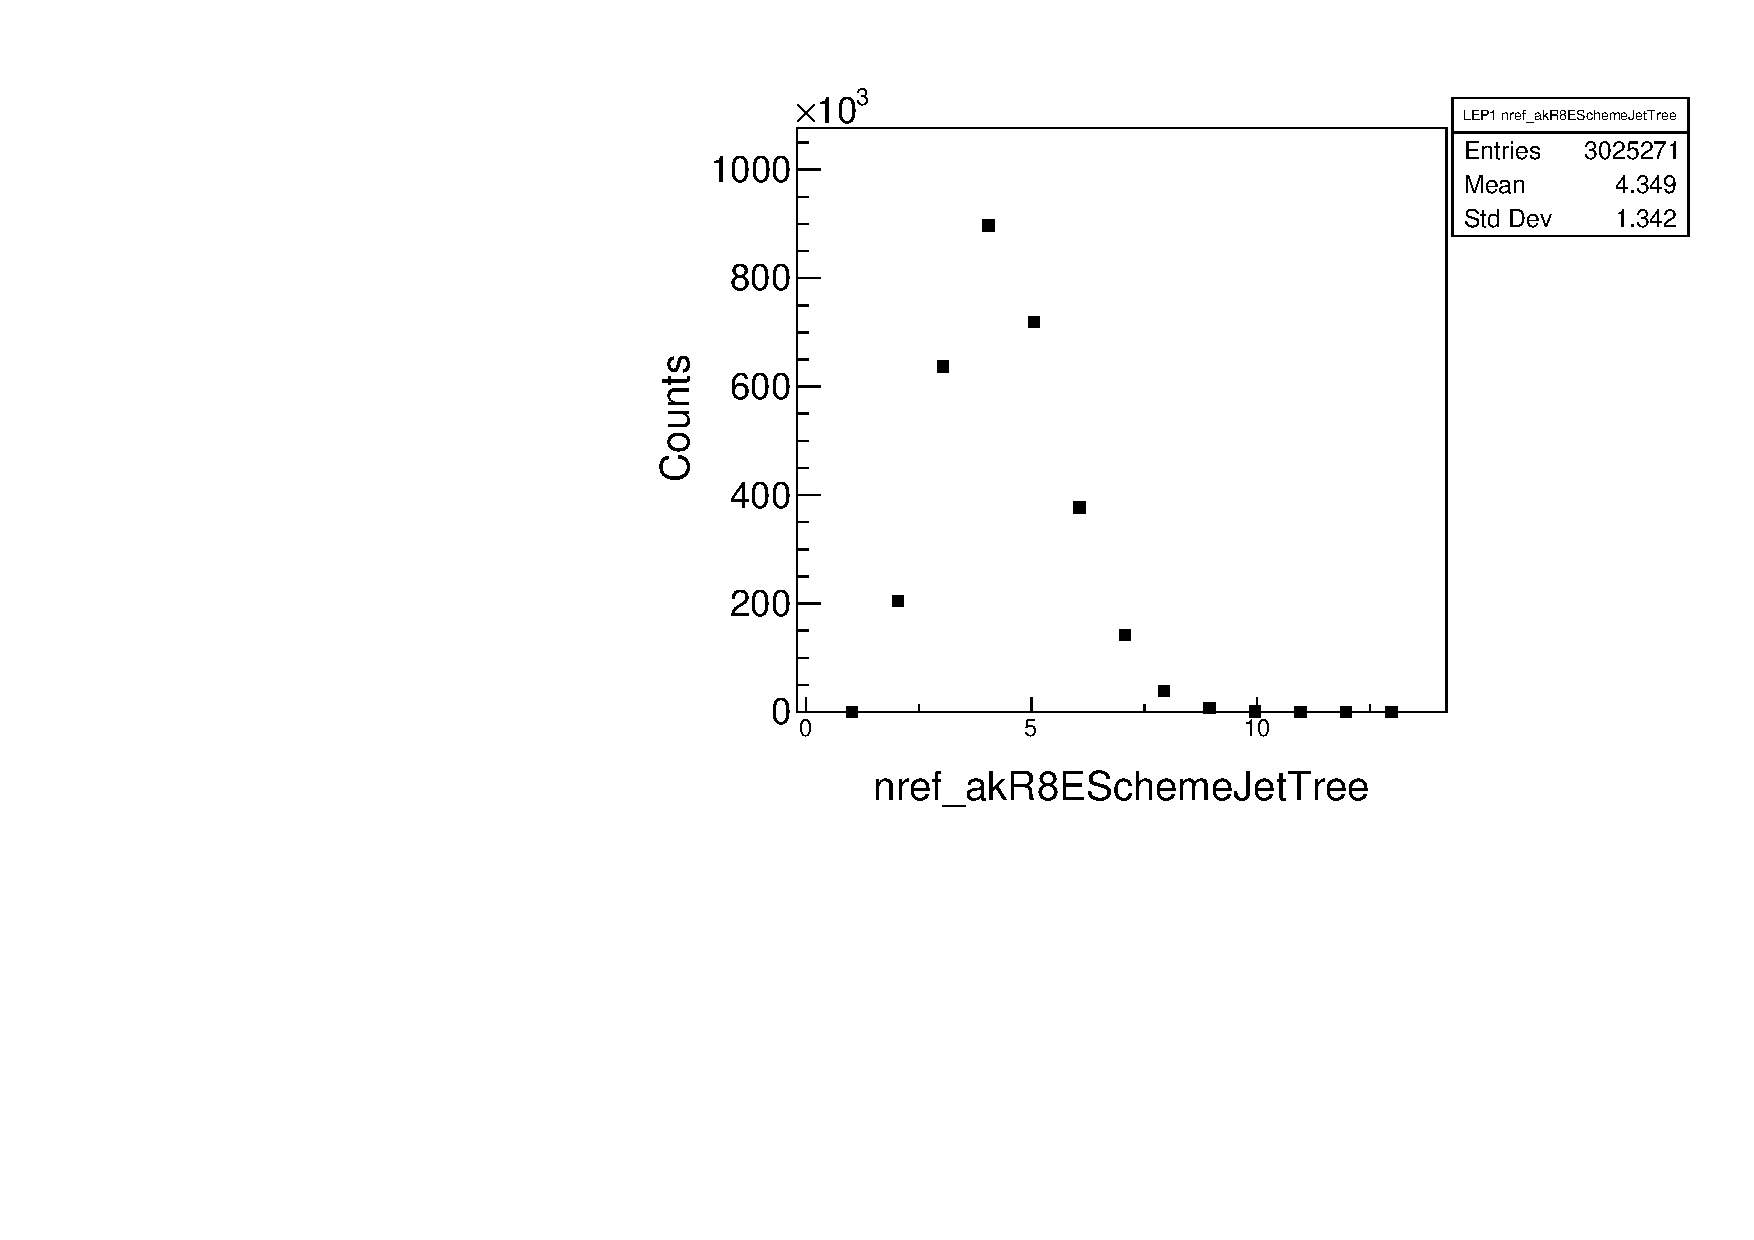
\includegraphics[width=.25\textwidth]{images/DQC/LEP1/nref_akR8ESchemeJetTree.pdf}}\hfill
\subfloat{\label{sfig:c}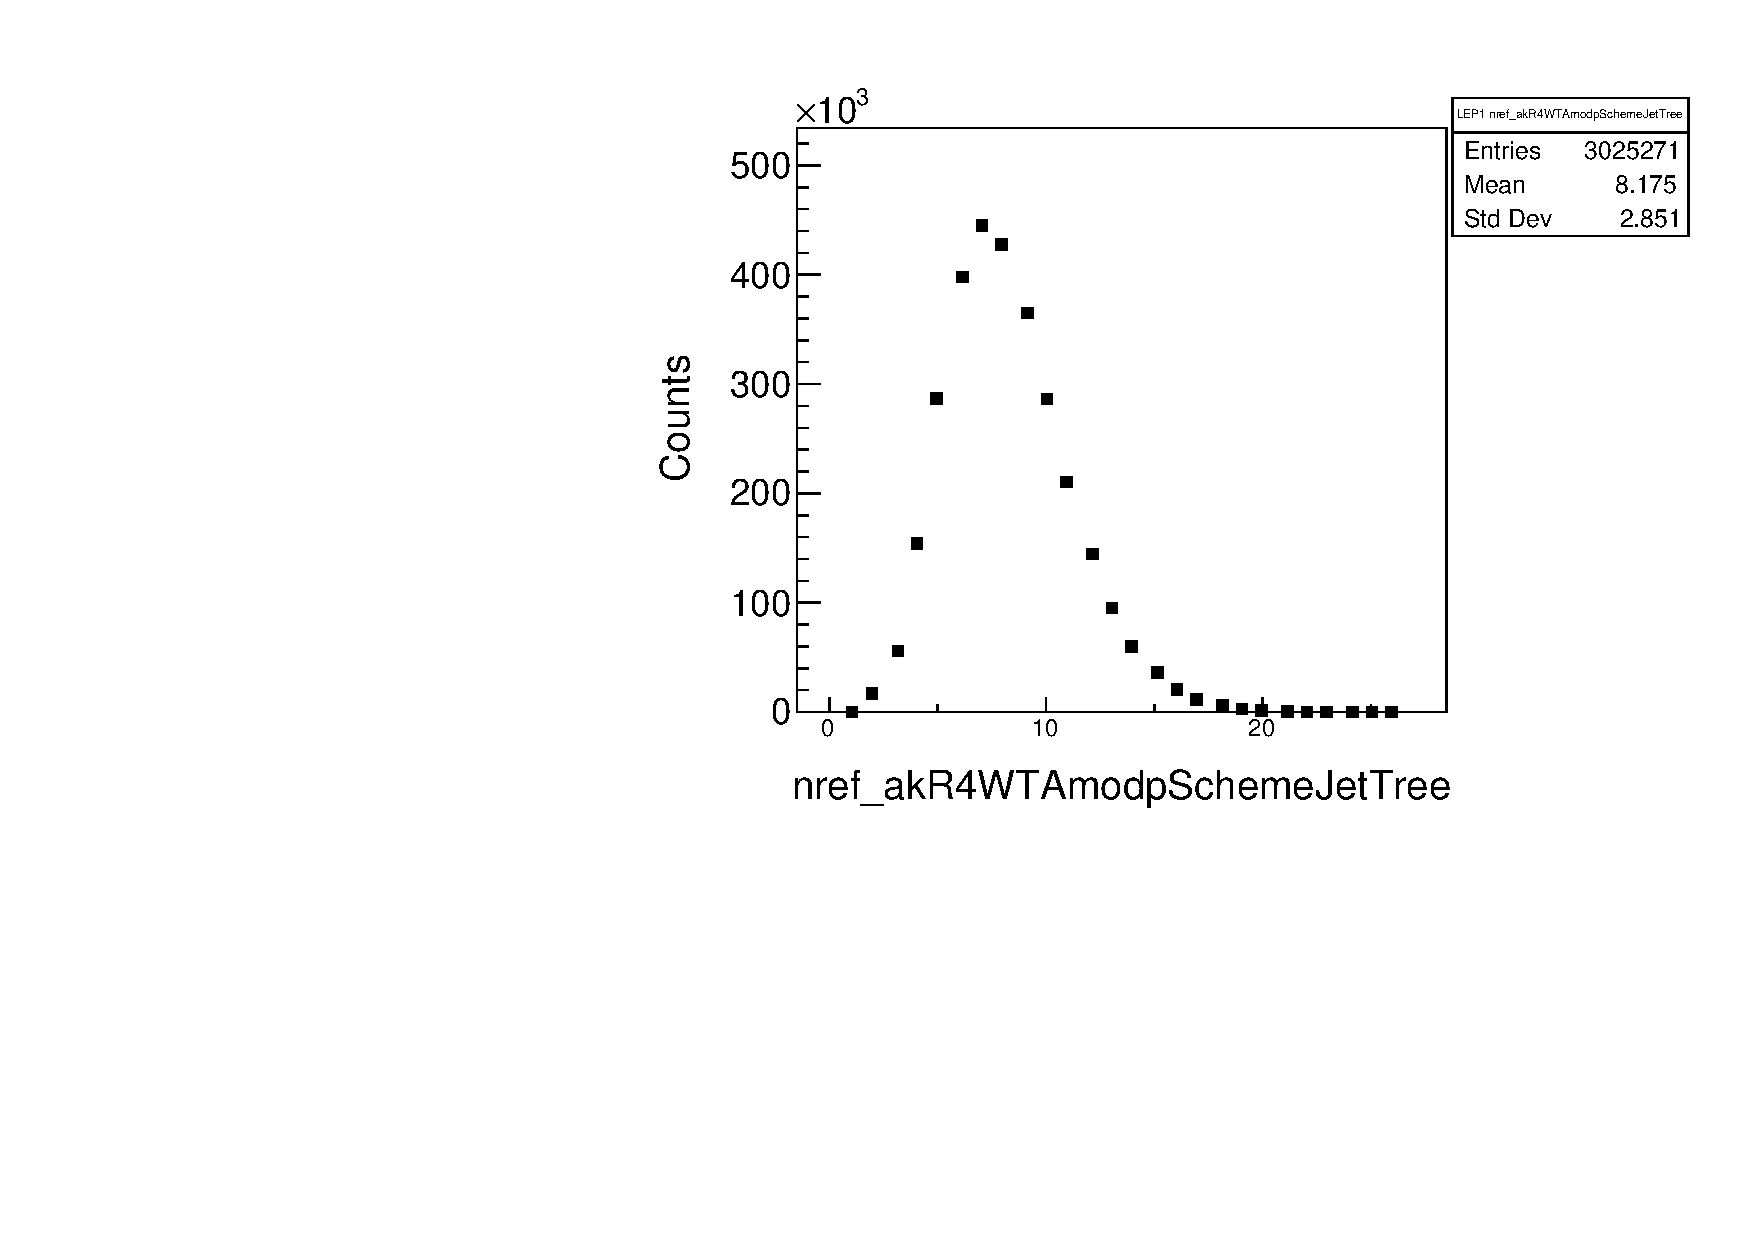
\includegraphics[width=.25\textwidth]{images/DQC/LEP1/nref_akR4WTAmodpSchemeJetTree.pdf}}\hfill
\subfloat{\label{sfig:d}\includegraphics[width=.25\textwidth]{images/DQC/LEP1/nref_akR8WTAmodpSchemeJetTree.pdf}}\hfill %row end
\subfloat{\label{sfig:e}\includegraphics[width=.25\textwidth]{images/DQC/LEP1/nref_ktN2ESchemeJetTree.pdf}}\hfill
\subfloat{\label{sfig:f}\includegraphics[width=.25\textwidth]{images/DQC/LEP1/nref_ktN3ESchemeJetTree.pdf}}\hfill
\subfloat{\label{sfig:g}\includegraphics[width=.25\textwidth]{images/DQC/LEP1/nref_ktN2WTAmodpSchemeJetTree.pdf}}\hfill
\subfloat{\label{sfig:h}\includegraphics[width=.25\textwidth]{images/DQC/LEP1/nref_ktN3WTAmodpSchemeJetTree.pdf}}\hfill
\caption{LEP1 Jet nref distributions. Top row: anti-$k_t$, left to right: $R=0.4$, $E$ scheme; $R=0.8$, $E$ scheme; $R=0.4$, WTA mod p scheme; $R=0.8$, WTA mod p scheme. Bottom row: $k_t$, left to right: $N=2$, $E$ scheme; $N=3$, $E$ scheme; $N=2$, WTA mod p scheme; $N=3$; WTA mod p scheme.}  
\end{figure}

\begin{figure}[H]
\centering
\subfloat{\label{sfig:a}\includegraphics[width=.33\textwidth]{images/DQC/LEP1/eta.pdf}}\hfill
\subfloat{\label{sfig:b}\includegraphics[width=.33\textwidth]{images/DQC/LEP1/eta_wrtThr.pdf}}\hfill
\subfloat{\label{sfig:c}\includegraphics[width=.33\textwidth]{images/DQC/LEP1/eta_wrtChThr.pdf}}\hfill
\caption{LEP1 $\eta$ distributions. Left to right: $\eta$; $\eta$ with respect to thrust axis; $\eta$ with respect to charged thrust axis.}
\end{figure}

\begin{figure}[H]
\centering
\subfloat{\label{sfig:a}\includegraphics[width=.33\textwidth]{images/DQC/LEP1/phi.pdf}}\hfill
\subfloat{\label{sfig:b}\includegraphics[width=.33\textwidth]{images/DQC/LEP1/phi_wrtThr.pdf}}\hfill
\subfloat{\label{sfig:c}\includegraphics[width=.33\textwidth]{images/DQC/LEP1/phi_wrtChThr.pdf}}\hfill
\caption{LEP1 $\phi$ distributions. Left to right: $\phi$; $\phi$ with respect to thrust axis; $\phi$ with respect to charged thrust axis.}
\end{figure}

\begin{figure}[H]
\centering
\subfloat{\label{sfig:a}\includegraphics[width=.33\textwidth]{images/DQC/LEP1/pt.pdf}}\hfill
\subfloat{\label{sfig:b}\includegraphics[width=.33\textwidth]{images/DQC/LEP1/pt_wrtThr.pdf}}\hfill
\subfloat{\label{sfig:c}\includegraphics[width=.33\textwidth]{images/DQC/LEP1/pt_wrtChThr.pdf}}\hfill
\caption{LEP1 $p_t$ distributions. Left to right: $p_t$; $p_t$ with respect to thrust axis; $p_t$ with respect to charged thrust axis.}
\end{figure}

\begin{figure}[H]
\centering
\subfloat{\label{sfig:a}\includegraphics[width=.33\textwidth]{images/DQC/LEP1/theta.pdf}}\hfill
\subfloat{\label{sfig:b}\includegraphics[width=.33\textwidth]{images/DQC/LEP1/theta_wrtThr.pdf}}\hfill
\subfloat{\label{sfig:c}\includegraphics[width=.33\textwidth]{images/DQC/LEP1/theta_wrtChThr.pdf}}\hfill
\caption{LEP1 $\theta$ distributions. Left to right: $\theta$; $\theta$ with respect to thrust axis; $\theta$ with respect to charged thrust axis.}
\end{figure}

\begin{figure}[H]
\centering
\subfloat{\label{sfig:a}\includegraphics[width=.25\textwidth]{images/DQC/LEP1/px.pdf}}\hfill
\subfloat{\label{sfig:b}\includegraphics[width=.25\textwidth]{images/DQC/LEP1/py.pdf}}\hfill
\subfloat{\label{sfig:c}\includegraphics[width=.25\textwidth]{images/DQC/LEP1/pz.pdf}}\hfill
\subfloat{\label{sfig:a}\includegraphics[width=.25\textwidth]{images/DQC/LEP1/pmag.pdf}}\hfill
\caption{LEP1 $p_x$, $p_y$, $p_z$, and $|\vec{p}|$ distributions.}
\end{figure}

\begin{figure}[H]
\centering
\subfloat{\label{sfig:a}\includegraphics[width=.25\textwidth]{images/DQC/LEP1/missP.pdf}}\hfill
\subfloat{\label{sfig:b}\includegraphics[width=.25\textwidth]{images/DQC/LEP1/missPt.pdf}}\hfill
\subfloat{\label{sfig:c}\includegraphics[width=.25\textwidth]{images/DQC/LEP1/missTheta.pdf}}\hfill
\subfloat{\label{sfig:d}\includegraphics[width=.25\textwidth]{images/DQC/LEP1/missPhi.pdf}}\hfill %row end
\subfloat{\label{sfig:e}\includegraphics[width=.25\textwidth]{images/DQC/LEP1/missChargedP.pdf}}\hfill
\subfloat{\label{sfig:f}\includegraphics[width=.25\textwidth]{images/DQC/LEP1/missChargedPt.pdf}}\hfill
\subfloat{\label{sfig:g}\includegraphics[width=.25\textwidth]{images/DQC/LEP1/missChargedTheta.pdf}}\hfill
\subfloat{\label{sfig:h}\includegraphics[width=.25\textwidth]{images/DQC/LEP1/missChargedPhi.pdf}}\hfill
\caption{LEP1 missing quantities distribution. Left to right: missing $P$; missing $p_t$; missing $\theta$; missing $\phi$. Top to bottom: All; charged.}  
\end{figure}

\begin{figure}[H]
\centering
\subfloat{\label{sfig:a}\includegraphics[width=.33\textwidth]{images/DQC/LEP1/charge.pdf}}\hfill
\subfloat{\label{sfig:b}\includegraphics[width=.33\textwidth]{images/DQC/LEP1/d0.pdf}}\hfill
\subfloat{\label{sfig:c}\includegraphics[width=.33\textwidth]{images/DQC/LEP1/Energy.pdf}}\hfill %row end
\subfloat{\label{sfig:d}\includegraphics[width=.33\textwidth]{images/DQC/LEP1/mass.pdf}}\hfill
\subfloat{\label{sfig:e}\includegraphics[width=.33\textwidth]{images/DQC/LEP1/nParticle.pdf}}\hfill
\subfloat{\label{sfig:f}\includegraphics[width=.33\textwidth]{images/DQC/LEP1/pwflag.pdf}}\hfill
\caption{Left to right: Top row: LEP1 charge, $d_0$, and energy distributions. Bottom row: LEP1 mass, particle multiplicity, and pwflag distributions.}
\end{figure}

\begin{figure}[H]
\centering
\subfloat{\label{sfig:a}\includegraphics[width=.5\textwidth]{images/DQC/LEP1/bx.pdf}}\hfill
\subfloat{\label{sfig:b}\includegraphics[width=.5\textwidth]{images/DQC/LEP1/by.pdf}}\hfill %row end
\subfloat{\label{sfig:c}\includegraphics[width=.5\textwidth]{images/DQC/LEP1/ebx.pdf}}\hfill
\subfloat{\label{sfig:d}\includegraphics[width=.5\textwidth]{images/DQC/LEP1/eby.pdf}}\hfill
\caption{Top row: LEP1 beamspot $x$ and $y$. Bottom row: Error in beamspot $x$ and $y$.}
\end{figure}

\begin{figure}[H]
\centering
\subfloat{\label{sfig:a}\includegraphics[width=.5\textwidth]{images/DQC/LEP1/Thrust.pdf}}\hfill
\subfloat{\label{sfig:b}\includegraphics[width=.5\textwidth]{images/DQC/LEP1/Thrust_charged.pdf}}\hfill %row end
\caption{Left: LEP1 thrust distribution. Right: LEP1 charged thrust distribution.}
\end{figure}

\begin{figure}[H]
\centering
\subfloat{\label{sfig:a}\includegraphics[width=.33\textwidth]{images/DQC/LEP1/nChargedHadrons.pdf}}\hfill
\subfloat{\label{sfig:b}\includegraphics[width=.33\textwidth]{images/DQC/LEP1/nChargedHadrons_GT0p4.pdf}}\hfill
\subfloat{\label{sfig:c}\includegraphics[width=.33\textwidth]{images/DQC/LEP1/nChargedHadrons_GT0p4Thrust.pdf}}\hfill
\caption{LEP1 charged hadron multiplicity distributions. Left to right: charged hadron multiplicity; charged hadron multiplicity (GT0p4); charged hadron multiplicity (GT0p4Thrust).}
\end{figure}

\begin{figure}[H]
\centering
\subfloat{\label{sfig:a}\includegraphics[width=.33\textwidth]{images/DQC/LEP1/z0.pdf}}\hfill
\subfloat{\label{sfig:b}\includegraphics[width=.33\textwidth]{images/DQC/LEP1/ntpc.pdf}}\hfill %row end
\subfloat{\label{sfig:c}\includegraphics[width=.33\textwidth]{images/DQC/LEP1/rap.pdf}}\hfill %row end
\caption{Left: LEP1 $z_0$ distribution. Center: LEP1 TPC hits distribution. Right: LEP1 rapidity distribution.}
\end{figure}

%%%%%%%%%%%%%%%%%%%%%%%%%%%%%%%%%%%% LEP 2 %%%%%%%%%%%%%%%%%%%%%%%%%%%%%%%%

\subsection{LEP2 Data}

\begin{comment}
\begin{figure}[!htb]
\begin{center}
\includegraphics[width=.45\textwidth]{images/DataQualityCheck/LEP2_eta.pdf}
\caption{LEP2 Eta Spectra}
\label{fig:figure4} 
\end{center}
\end{figure}

\begin{figure}[!htb]
\begin{center}
\includegraphics[width=.45\textwidth]{images/DataQualityCheck/LEP2_pt.pdf}
\caption{LEP2 PT spectra}
\label{fig:figure5} 
\end{center}
\end{figure}

\begin{figure}[!htb]
\begin{center}
\includegraphics[width=.45\textwidth]{images/DataQualityCheck/LEP2_mult.pdf}
\caption{LEP2 Multiplicity Distribution}
\label{fig:figure6} 
\end{center}
\end{figure}
\end{comment}

\begin{figure}[H]
\centering
\subfloat{\label{sfig:a}\includegraphics[width=.25\textwidth]{images/DQC/LEP2/jteta_akR4ESchemeJetTree.pdf}}\hfill
\subfloat{\label{sfig:b}\includegraphics[width=.25\textwidth]{images/DQC/LEP2/jteta_akR8ESchemeJetTree.pdf}}\hfill
\subfloat{\label{sfig:c}\includegraphics[width=.25\textwidth]{images/DQC/LEP2/jteta_akR4WTAmodpSchemeJetTree.pdf}}\hfill
\subfloat{\label{sfig:d}\includegraphics[width=.25\textwidth]{images/DQC/LEP2/jteta_akR8WTAmodpSchemeJetTree.pdf}}\hfill %row end
\subfloat{\label{sfig:e}\includegraphics[width=.25\textwidth]{images/DQC/LEP2/jteta_ktN2ESchemeJetTree.pdf}}\hfill
\subfloat{\label{sfig:f}\includegraphics[width=.25\textwidth]{images/DQC/LEP2/jteta_ktN3ESchemeJetTree.pdf}}\hfill
\subfloat{\label{sfig:g}\includegraphics[width=.25\textwidth]{images/DQC/LEP2/jteta_ktN2WTAmodpSchemeJetTree.pdf}}\hfill
\subfloat{\label{sfig:h}\includegraphics[width=.25\textwidth]{images/DQC/LEP2/jteta_ktN3WTAmodpSchemeJetTree.pdf}}\hfill
\caption{LEP2 Jet $\eta$ distributions. Top row: anti-$k_t$, left to right: $R=0.4$, $E$ scheme; $R=0.8$, $E$ scheme; $R=0.4$, WTA mod p scheme; $R=0.8$, WTA mod p scheme. Bottom row: $k_t$, left to right: $N=2$, $E$ scheme; $N=3$, $E$ scheme; $N=2$, WTA mod p scheme; $N=3$; WTA mod p scheme.}  
\end{figure}

\begin{figure}[H]
\centering
\subfloat{\label{sfig:a}\includegraphics[width=.25\textwidth]{images/DQC/LEP2/jtphi_akR4ESchemeJetTree.pdf}}\hfill
\subfloat{\label{sfig:b}\includegraphics[width=.25\textwidth]{images/DQC/LEP2/jtphi_akR8ESchemeJetTree.pdf}}\hfill
\subfloat{\label{sfig:c}\includegraphics[width=.25\textwidth]{images/DQC/LEP2/jtphi_akR4WTAmodpSchemeJetTree.pdf}}\hfill
\subfloat{\label{sfig:d}\includegraphics[width=.25\textwidth]{images/DQC/LEP2/jtphi_akR8WTAmodpSchemeJetTree.pdf}}\hfill %row end
\subfloat{\label{sfig:e}\includegraphics[width=.25\textwidth]{images/DQC/LEP2/jtphi_ktN2ESchemeJetTree.pdf}}\hfill
\subfloat{\label{sfig:f}\includegraphics[width=.25\textwidth]{images/DQC/LEP2/jtphi_ktN3ESchemeJetTree.pdf}}\hfill
\subfloat{\label{sfig:g}\includegraphics[width=.25\textwidth]{images/DQC/LEP2/jtphi_ktN2WTAmodpSchemeJetTree.pdf}}\hfill
\subfloat{\label{sfig:h}\includegraphics[width=.25\textwidth]{images/DQC/LEP2/jtphi_ktN3WTAmodpSchemeJetTree.pdf}}\hfill
\caption{LEP2 Jet $\phi$ distributions. Top row: anti-$k_t$, left to right: $R=0.4$, $E$ scheme; $R=0.8$, $E$ scheme; $R=0.4$, WTA mod p scheme; $R=0.8$, WTA mod p scheme. Bottom row: $k_t$, left to right: $N=2$, $E$ scheme; $N=3$, $E$ scheme; $N=2$, WTA mod p scheme; $N=3$; WTA mod p scheme.}  
\end{figure}

\begin{figure}[H]
\centering
\subfloat{\label{sfig:a}\includegraphics[width=.25\textwidth]{images/DQC/LEP2/jtpt_akR4ESchemeJetTree.pdf}}\hfill
\subfloat{\label{sfig:b}\includegraphics[width=.25\textwidth]{images/DQC/LEP2/jtpt_akR8ESchemeJetTree.pdf}}\hfill
\subfloat{\label{sfig:c}\includegraphics[width=.25\textwidth]{images/DQC/LEP2/jtpt_akR4WTAmodpSchemeJetTree.pdf}}\hfill
\subfloat{\label{sfig:d}\includegraphics[width=.25\textwidth]{images/DQC/LEP2/jtpt_akR8WTAmodpSchemeJetTree.pdf}}\hfill %row end
\subfloat{\label{sfig:e}\includegraphics[width=.25\textwidth]{images/DQC/LEP2/jtpt_ktN2ESchemeJetTree.pdf}}\hfill
\subfloat{\label{sfig:f}\includegraphics[width=.25\textwidth]{images/DQC/LEP2/jtpt_ktN3ESchemeJetTree.pdf}}\hfill
\subfloat{\label{sfig:g}\includegraphics[width=.25\textwidth]{images/DQC/LEP2/jtpt_ktN2WTAmodpSchemeJetTree.pdf}}\hfill
\subfloat{\label{sfig:h}\includegraphics[width=.25\textwidth]{images/DQC/LEP2/jtpt_ktN3WTAmodpSchemeJetTree.pdf}}\hfill
\caption{LEP2 Jet $p_t$ distributions. Top row: anti-$k_t$, left to right: $R=0.4$, $E$ scheme; $R=0.8$, $E$ scheme; $R=0.4$, WTA mod p scheme; $R=0.8$, WTA mod p scheme. Bottom row: $k_t$, left to right: $N=2$, $E$ scheme; $N=3$, $E$ scheme; $N=2$, WTA mod p scheme; $N=3$; WTA mod p scheme.}  
\end{figure}

\begin{figure}[H]
\centering
\subfloat{\label{sfig:a}\includegraphics[width=.25\textwidth]{images/DQC/LEP2/jtm_akR4ESchemeJetTree.pdf}}\hfill
\subfloat{\label{sfig:b}\includegraphics[width=.25\textwidth]{images/DQC/LEP2/jtm_akR8ESchemeJetTree.pdf}}\hfill
\subfloat{\label{sfig:c}\includegraphics[width=.25\textwidth]{images/DQC/LEP2/jtm_akR4WTAmodpSchemeJetTree.pdf}}\hfill
\subfloat{\label{sfig:d}\includegraphics[width=.25\textwidth]{images/DQC/LEP2/jtm_akR8WTAmodpSchemeJetTree.pdf}}\hfill %row end
\subfloat{\label{sfig:e}\includegraphics[width=.25\textwidth]{images/DQC/LEP2/jtm_ktN2ESchemeJetTree.pdf}}\hfill
\subfloat{\label{sfig:f}\includegraphics[width=.25\textwidth]{images/DQC/LEP2/jtm_ktN3ESchemeJetTree.pdf}}\hfill
\subfloat{\label{sfig:g}\includegraphics[width=.25\textwidth]{images/DQC/LEP2/jtm_ktN2WTAmodpSchemeJetTree.pdf}}\hfill
\subfloat{\label{sfig:h}\includegraphics[width=.25\textwidth]{images/DQC/LEP2/jtm_ktN3WTAmodpSchemeJetTree.pdf}}\hfill
\caption{LEP2 Jet mass distributions. Top row: anti-$k_t$, left to right: $R=0.4$, $E$ scheme; $R=0.8$, $E$ scheme; $R=0.4$, WTA mod p scheme; $R=0.8$, WTA mod p scheme. Bottom row: $k_t$, left to right: $N=2$, $E$ scheme; $N=3$, $E$ scheme; $N=2$, WTA mod p scheme; $N=3$; WTA mod p scheme.}  
\end{figure}

\begin{figure}[H]
\centering
\subfloat{\label{sfig:a}\includegraphics[width=.25\textwidth]{images/DQC/LEP2/jtN_akR4ESchemeJetTree.pdf}}\hfill
\subfloat{\label{sfig:b}\includegraphics[width=.25\textwidth]{images/DQC/LEP2/jtN_akR8ESchemeJetTree.pdf}}\hfill
\subfloat{\label{sfig:c}\includegraphics[width=.25\textwidth]{images/DQC/LEP2/jtN_akR4WTAmodpSchemeJetTree.pdf}}\hfill
\subfloat{\label{sfig:d}\includegraphics[width=.25\textwidth]{images/DQC/LEP2/jtN_akR8WTAmodpSchemeJetTree.pdf}}\hfill %row end
\subfloat{\label{sfig:e}\includegraphics[width=.25\textwidth]{images/DQC/LEP2/jtN_ktN2ESchemeJetTree.pdf}}\hfill
\subfloat{\label{sfig:f}\includegraphics[width=.25\textwidth]{images/DQC/LEP2/jtN_ktN3ESchemeJetTree.pdf}}\hfill
\subfloat{\label{sfig:g}\includegraphics[width=.25\textwidth]{images/DQC/LEP2/jtN_ktN2WTAmodpSchemeJetTree.pdf}}\hfill
\subfloat{\label{sfig:h}\includegraphics[width=.25\textwidth]{images/DQC/LEP2/jtN_ktN3WTAmodpSchemeJetTree.pdf}}\hfill
\caption{LEP2 Jet $N$ distributions. Top row: anti-$k_t$, left to right: $R=0.4$, $E$ scheme; $R=0.8$, $E$ scheme; $R=0.4$, WTA mod p scheme; $R=0.8$, WTA mod p scheme. Bottom row: $k_t$, left to right: $N=2$, $E$ scheme; $N=3$, $E$ scheme; $N=2$, WTA mod p scheme; $N=3$; WTA mod p scheme.}  
\end{figure} 

\begin{figure}[H]
\centering
\subfloat{\label{sfig:a}\includegraphics[width=.25\textwidth]{images/DQC/LEP2/nref_akR4ESchemeJetTree.pdf}}\hfill
\subfloat{\label{sfig:b}\includegraphics[width=.25\textwidth]{images/DQC/LEP2/nref_akR8ESchemeJetTree.pdf}}\hfill
\subfloat{\label{sfig:c}\includegraphics[width=.25\textwidth]{images/DQC/LEP2/nref_akR4WTAmodpSchemeJetTree.pdf}}\hfill
\subfloat{\label{sfig:d}\includegraphics[width=.25\textwidth]{images/DQC/LEP2/nref_akR8WTAmodpSchemeJetTree.pdf}}\hfill %row end
\subfloat{\label{sfig:e}\includegraphics[width=.25\textwidth]{images/DQC/LEP2/nref_ktN2ESchemeJetTree.pdf}}\hfill
\subfloat{\label{sfig:f}\includegraphics[width=.25\textwidth]{images/DQC/LEP2/nref_ktN3ESchemeJetTree.pdf}}\hfill
\subfloat{\label{sfig:g}\includegraphics[width=.25\textwidth]{images/DQC/LEP2/nref_ktN2WTAmodpSchemeJetTree.pdf}}\hfill
\subfloat{\label{sfig:h}\includegraphics[width=.25\textwidth]{images/DQC/LEP2/nref_ktN3WTAmodpSchemeJetTree.pdf}}\hfill
\caption{LEP2 Jet nref distributions. Top row: anti-$k_t$, left to right: $R=0.4$, $E$ scheme; $R=0.8$, $E$ scheme; $R=0.4$, WTA mod p scheme; $R=0.8$, WTA mod p scheme. Bottom row: $k_t$, left to right: $N=2$, $E$ scheme; $N=3$, $E$ scheme; $N=2$, WTA mod p scheme; $N=3$; WTA mod p scheme.}  
\end{figure}

\begin{figure}[H]
\centering
\subfloat{\label{sfig:a}\includegraphics[width=.33\textwidth]{images/DQC/LEP2/eta.pdf}}\hfill
\subfloat{\label{sfig:b}\includegraphics[width=.33\textwidth]{images/DQC/LEP2/eta_wrtThr.pdf}}\hfill
\subfloat{\label{sfig:c}\includegraphics[width=.33\textwidth]{images/DQC/LEP2/eta_wrtChThr.pdf}}\hfill
\caption{LEP2 $\eta$ distributions. Left to right: $\eta$; $\eta$ with respect to thrust axis; $\eta$ with respect to charged thrust axis.}
\end{figure}

\begin{figure}[H]
\centering
\subfloat{\label{sfig:a}\includegraphics[width=.33\textwidth]{images/DQC/LEP2/phi.pdf}}\hfill
\subfloat{\label{sfig:b}\includegraphics[width=.33\textwidth]{images/DQC/LEP2/phi_wrtThr.pdf}}\hfill
\subfloat{\label{sfig:c}\includegraphics[width=.33\textwidth]{images/DQC/LEP2/phi_wrtChThr.pdf}}\hfill
\caption{LEP2 $\phi$ distributions. Left to right: $\phi$; $\phi$ with respect to thrust axis; $\phi$ with respect to charged thrust axis.}
\end{figure}

\begin{figure}[H]
\centering
\subfloat{\label{sfig:a}\includegraphics[width=.33\textwidth]{images/DQC/LEP2/pt.pdf}}\hfill
\subfloat{\label{sfig:b}\includegraphics[width=.33\textwidth]{images/DQC/LEP2/pt_wrtThr.pdf}}\hfill
\subfloat{\label{sfig:c}\includegraphics[width=.33\textwidth]{images/DQC/LEP2/pt_wrtChThr.pdf}}\hfill
\caption{LEP2 $p_t$ distributions. Left to right: $p_t$; $p_t$ with respect to thrust axis; $p_t$ with respect to charged thrust axis.}
\end{figure}

\begin{figure}[H]
\centering
\subfloat{\label{sfig:a}\includegraphics[width=.33\textwidth]{images/DQC/LEP2/theta.pdf}}\hfill
\subfloat{\label{sfig:b}\includegraphics[width=.33\textwidth]{images/DQC/LEP2/theta_wrtThr.pdf}}\hfill
\subfloat{\label{sfig:c}\includegraphics[width=.33\textwidth]{images/DQC/LEP2/theta_wrtChThr.pdf}}\hfill
\caption{LEP2 $\theta$ distributions. Left to right: $\theta$; $\theta$ with respect to thrust axis; $\theta$ with respect to charged thrust axis.}
\end{figure}

\begin{figure}[H]
\centering
\subfloat{\label{sfig:a}\includegraphics[width=.25\textwidth]{images/DQC/LEP2/px.pdf}}\hfill
\subfloat{\label{sfig:b}\includegraphics[width=.25\textwidth]{images/DQC/LEP2/py.pdf}}\hfill
\subfloat{\label{sfig:c}\includegraphics[width=.25\textwidth]{images/DQC/LEP2/pz.pdf}}\hfill
\subfloat{\label{sfig:a}\includegraphics[width=.25\textwidth]{images/DQC/LEP2/pmag.pdf}}\hfill
\caption{LEP2 $p_x$, $p_y$, $p_z$, and $|\vec{p}|$ distributions.}
\end{figure}

\begin{figure}[H]
\centering
\subfloat{\label{sfig:a}\includegraphics[width=.25\textwidth]{images/DQC/LEP2/missP.pdf}}\hfill
\subfloat{\label{sfig:b}\includegraphics[width=.25\textwidth]{images/DQC/LEP2/missPt.pdf}}\hfill
\subfloat{\label{sfig:c}\includegraphics[width=.25\textwidth]{images/DQC/LEP2/missTheta.pdf}}\hfill
\subfloat{\label{sfig:d}\includegraphics[width=.25\textwidth]{images/DQC/LEP2/missPhi.pdf}}\hfill %row end
\subfloat{\label{sfig:e}\includegraphics[width=.25\textwidth]{images/DQC/LEP2/missChargedP.pdf}}\hfill
\subfloat{\label{sfig:f}\includegraphics[width=.25\textwidth]{images/DQC/LEP2/missChargedPt.pdf}}\hfill
\subfloat{\label{sfig:g}\includegraphics[width=.25\textwidth]{images/DQC/LEP2/missChargedTheta.pdf}}\hfill
\subfloat{\label{sfig:h}\includegraphics[width=.25\textwidth]{images/DQC/LEP2/missChargedPhi.pdf}}\hfill
\caption{LEP2 missing quantities distribution. Left to right: missing $P$; missing $p_t$; missing $\theta$; missing $\phi$. Top to bottom: All; charged.}  
\end{figure}

\begin{figure}[H]
\centering
\subfloat{\label{sfig:a}\includegraphics[width=.33\textwidth]{images/DQC/LEP2/charge.pdf}}\hfill
\subfloat{\label{sfig:b}\includegraphics[width=.33\textwidth]{images/DQC/LEP2/d0.pdf}}\hfill
\subfloat{\label{sfig:c}\includegraphics[width=.33\textwidth]{images/DQC/LEP2/Energy.pdf}}\hfill %row end
\subfloat{\label{sfig:d}\includegraphics[width=.33\textwidth]{images/DQC/LEP2/mass.pdf}}\hfill
\subfloat{\label{sfig:e}\includegraphics[width=.33\textwidth]{images/DQC/LEP2/nParticle.pdf}}\hfill
\subfloat{\label{sfig:f}\includegraphics[width=.33\textwidth]{images/DQC/LEP2/pwflag.pdf}}\hfill
\caption{Left to right: Top row: LEP2 charge, $d_0$, and energy distributions. Bottom row: LEP2 mass, particle multiplicity, and pwflag distributions.}
\end{figure}

\begin{figure}[H]
\centering
\subfloat{\label{sfig:a}\includegraphics[width=.5\textwidth]{images/DQC/LEP2/bx.pdf}}\hfill
\subfloat{\label{sfig:b}\includegraphics[width=.5\textwidth]{images/DQC/LEP2/by.pdf}}\hfill %row end
\subfloat{\label{sfig:c}\includegraphics[width=.5\textwidth]{images/DQC/LEP2/ebx.pdf}}\hfill
\subfloat{\label{sfig:d}\includegraphics[width=.5\textwidth]{images/DQC/LEP2/eby.pdf}}\hfill
\caption{Top row: LEP2 beamspot $x$ and $y$. Bottom row: Error in beamspot $x$ and $y$.}
\end{figure}

\begin{figure}[H]
\centering
\subfloat{\label{sfig:a}\includegraphics[width=.5\textwidth]{images/DQC/LEP2/Thrust.pdf}}\hfill
\subfloat{\label{sfig:b}\includegraphics[width=.5\textwidth]{images/DQC/LEP2/Thrust_charged.pdf}}\hfill %row end
\caption{Left: LEP2 thrust distribution. Right: LEP2 charged thrust distribution.}
\end{figure}

\begin{figure}[H]
\centering
\subfloat{\label{sfig:a}\includegraphics[width=.33\textwidth]{images/DQC/LEP2/nChargedHadrons.pdf}}\hfill
\subfloat{\label{sfig:b}\includegraphics[width=.33\textwidth]{images/DQC/LEP2/nChargedHadrons_GT0p4.pdf}}\hfill
\subfloat{\label{sfig:c}\includegraphics[width=.33\textwidth]{images/DQC/LEP2/nChargedHadrons_GT0p4Thrust.pdf}}\hfill
\caption{LEP2 charged hadron multiplicity distributions. Left to right: charged hadron multiplicity; charged hadron multiplicity (GT0p4); charged hadron multiplicity (GT0p4Thrust).}
\end{figure}

\begin{figure}[H]
\centering
\subfloat{\label{sfig:a}\includegraphics[width=.33\textwidth]{images/DQC/LEP2/z0.pdf}}\hfill
\subfloat{\label{sfig:b}\includegraphics[width=.33\textwidth]{images/DQC/LEP2/ntpc.pdf}}\hfill %row end
\subfloat{\label{sfig:c}\includegraphics[width=.33\textwidth]{images/DQC/LEP2/rap.pdf}}\hfill %row end
\caption{Left: LEP2 $z_0$ distribution. Center: LEP2 TPC hits distribution. Right: LEP2 rapidity distribution.}
\end{figure}

%%%%%%%%%%%%%%%%%%%%%%%%%%%%%%%%%%%% PYTHIA8 %%%%%%%%%%%%%%%%%%%%%%%%%%%%%%%%

\subsection{PYTHIA8 Sample}

Note that the plots below only utilize a small subset of the PYTHIA8 results.

\begin{comment}
\begin{figure}[H]
\begin{center}
\includegraphics[width=.45\textwidth]{images/DataQualityCheck/PYTHIA8_eta.pdf}
\caption{PYTHIA8 Eta Spectra}
\label{fig:figure7} 
\end{center}
\end{figure}

\begin{figure}[H]
\begin{center}
\includegraphics[width=.45\textwidth]{images/DataQualityCheck/PYTHIA8_pt.pdf}
\caption{PYTHIA8 PT spectra}
\label{fig:figure8} 
\end{center}
\end{figure}

\begin{figure}[H]
\begin{center}
\includegraphics[width=.45\textwidth]{images/DataQualityCheck/PYTHIA8_mult.pdf}
\caption{PYTHIA8 Multiplicity Distribution}
\label{fig:figure9} 
\end{center}
\end{figure}
\end{comment}

\begin{figure}[H]
\centering
\subfloat{\label{sfig:a}\includegraphics[width=.25\textwidth]{images/DQC/PYTHIA8/jteta_akR4ESchemeJetTree.pdf}}\hfill
\subfloat{\label{sfig:b}\includegraphics[width=.25\textwidth]{images/DQC/PYTHIA8/jteta_akR8ESchemeJetTree.pdf}}\hfill
\subfloat{\label{sfig:c}\includegraphics[width=.25\textwidth]{images/DQC/PYTHIA8/jteta_akR4WTAmodpSchemeJetTree.pdf}}\hfill
\subfloat{\label{sfig:d}\includegraphics[width=.25\textwidth]{images/DQC/PYTHIA8/jteta_akR8WTAmodpSchemeJetTree.pdf}}\hfill %row end
\subfloat{\label{sfig:e}\includegraphics[width=.25\textwidth]{images/DQC/PYTHIA8/jteta_ktN2ESchemeJetTree.pdf}}\hfill
\subfloat{\label{sfig:f}\includegraphics[width=.25\textwidth]{images/DQC/PYTHIA8/jteta_ktN3ESchemeJetTree.pdf}}\hfill
\subfloat{\label{sfig:g}\includegraphics[width=.25\textwidth]{images/DQC/PYTHIA8/jteta_ktN2WTAmodpSchemeJetTree.pdf}}\hfill
\subfloat{\label{sfig:h}\includegraphics[width=.25\textwidth]{images/DQC/PYTHIA8/jteta_ktN3WTAmodpSchemeJetTree.pdf}}\hfill
\caption{PYTHIA8 Jet $\eta$ distributions. Top row: anti-$k_t$, left to right: $R=0.4$, $E$ scheme; $R=0.8$, $E$ scheme; $R=0.4$, WTA mod p scheme; $R=0.8$, WTA mod p scheme. Bottom row: $k_t$, left to right: $N=2$, $E$ scheme; $N=3$, $E$ scheme; $N=2$, WTA mod p scheme; $N=3$; WTA mod p scheme.}  
\end{figure}

\begin{figure}[H]
\centering
\subfloat{\label{sfig:a}\includegraphics[width=.25\textwidth]{images/DQC/PYTHIA8/jtphi_akR4ESchemeJetTree.pdf}}\hfill
\subfloat{\label{sfig:b}\includegraphics[width=.25\textwidth]{images/DQC/PYTHIA8/jtphi_akR8ESchemeJetTree.pdf}}\hfill
\subfloat{\label{sfig:c}\includegraphics[width=.25\textwidth]{images/DQC/PYTHIA8/jtphi_akR4WTAmodpSchemeJetTree.pdf}}\hfill
\subfloat{\label{sfig:d}\includegraphics[width=.25\textwidth]{images/DQC/PYTHIA8/jtphi_akR8WTAmodpSchemeJetTree.pdf}}\hfill %row end
\subfloat{\label{sfig:e}\includegraphics[width=.25\textwidth]{images/DQC/PYTHIA8/jtphi_ktN2ESchemeJetTree.pdf}}\hfill
\subfloat{\label{sfig:f}\includegraphics[width=.25\textwidth]{images/DQC/PYTHIA8/jtphi_ktN3ESchemeJetTree.pdf}}\hfill
\subfloat{\label{sfig:g}\includegraphics[width=.25\textwidth]{images/DQC/PYTHIA8/jtphi_ktN2WTAmodpSchemeJetTree.pdf}}\hfill
\subfloat{\label{sfig:h}\includegraphics[width=.25\textwidth]{images/DQC/PYTHIA8/jtphi_ktN3WTAmodpSchemeJetTree.pdf}}\hfill
\caption{PYTHIA8 Jet $\phi$ distributions. Top row: anti-$k_t$, left to right: $R=0.4$, $E$ scheme; $R=0.8$, $E$ scheme; $R=0.4$, WTA mod p scheme; $R=0.8$, WTA mod p scheme. Bottom row: $k_t$, left to right: $N=2$, $E$ scheme; $N=3$, $E$ scheme; $N=2$, WTA mod p scheme; $N=3$; WTA mod p scheme.}  
\end{figure}

\begin{figure}[H]
\centering
\subfloat{\label{sfig:a}\includegraphics[width=.25\textwidth]{images/DQC/PYTHIA8/jtpt_akR4ESchemeJetTree.pdf}}\hfill
\subfloat{\label{sfig:b}\includegraphics[width=.25\textwidth]{images/DQC/PYTHIA8/jtpt_akR8ESchemeJetTree.pdf}}\hfill
\subfloat{\label{sfig:c}\includegraphics[width=.25\textwidth]{images/DQC/PYTHIA8/jtpt_akR4WTAmodpSchemeJetTree.pdf}}\hfill
\subfloat{\label{sfig:d}\includegraphics[width=.25\textwidth]{images/DQC/PYTHIA8/jtpt_akR8WTAmodpSchemeJetTree.pdf}}\hfill %row end
\subfloat{\label{sfig:e}\includegraphics[width=.25\textwidth]{images/DQC/PYTHIA8/jtpt_ktN2ESchemeJetTree.pdf}}\hfill
\subfloat{\label{sfig:f}\includegraphics[width=.25\textwidth]{images/DQC/PYTHIA8/jtpt_ktN3ESchemeJetTree.pdf}}\hfill
\subfloat{\label{sfig:g}\includegraphics[width=.25\textwidth]{images/DQC/PYTHIA8/jtpt_ktN2WTAmodpSchemeJetTree.pdf}}\hfill
\subfloat{\label{sfig:h}\includegraphics[width=.25\textwidth]{images/DQC/PYTHIA8/jtpt_ktN3WTAmodpSchemeJetTree.pdf}}\hfill
\caption{PYTHIA8 Jet $p_t$ distributions. Top row: anti-$k_t$, left to right: $R=0.4$, $E$ scheme; $R=0.8$, $E$ scheme; $R=0.4$, WTA mod p scheme; $R=0.8$, WTA mod p scheme. Bottom row: $k_t$, left to right: $N=2$, $E$ scheme; $N=3$, $E$ scheme; $N=2$, WTA mod p scheme; $N=3$; WTA mod p scheme.}  
\end{figure}

\begin{figure}[H]
\centering
\subfloat{\label{sfig:a}\includegraphics[width=.25\textwidth]{images/DQC/PYTHIA8/jtm_akR4ESchemeJetTree.pdf}}\hfill
\subfloat{\label{sfig:b}\includegraphics[width=.25\textwidth]{images/DQC/PYTHIA8/jtm_akR8ESchemeJetTree.pdf}}\hfill
\subfloat{\label{sfig:c}\includegraphics[width=.25\textwidth]{images/DQC/PYTHIA8/jtm_akR4WTAmodpSchemeJetTree.pdf}}\hfill
\subfloat{\label{sfig:d}\includegraphics[width=.25\textwidth]{images/DQC/PYTHIA8/jtm_akR8WTAmodpSchemeJetTree.pdf}}\hfill %row end
\subfloat{\label{sfig:e}\includegraphics[width=.25\textwidth]{images/DQC/PYTHIA8/jtm_ktN2ESchemeJetTree.pdf}}\hfill
\subfloat{\label{sfig:f}\includegraphics[width=.25\textwidth]{images/DQC/PYTHIA8/jtm_ktN3ESchemeJetTree.pdf}}\hfill
\subfloat{\label{sfig:g}\includegraphics[width=.25\textwidth]{images/DQC/PYTHIA8/jtm_ktN2WTAmodpSchemeJetTree.pdf}}\hfill
\subfloat{\label{sfig:h}\includegraphics[width=.25\textwidth]{images/DQC/PYTHIA8/jtm_ktN3WTAmodpSchemeJetTree.pdf}}\hfill
\caption{PYTHIA8 Jet mass distributions. Top row: anti-$k_t$, left to right: $R=0.4$, $E$ scheme; $R=0.8$, $E$ scheme; $R=0.4$, WTA mod p scheme; $R=0.8$, WTA mod p scheme. Bottom row: $k_t$, left to right: $N=2$, $E$ scheme; $N=3$, $E$ scheme; $N=2$, WTA mod p scheme; $N=3$; WTA mod p scheme.}  
\end{figure}

\begin{figure}[H]
\centering
\subfloat{\label{sfig:a}\includegraphics[width=.25\textwidth]{images/DQC/PYTHIA8/jtN_akR4ESchemeJetTree.pdf}}\hfill
\subfloat{\label{sfig:b}\includegraphics[width=.25\textwidth]{images/DQC/PYTHIA8/jtN_akR8ESchemeJetTree.pdf}}\hfill
\subfloat{\label{sfig:c}\includegraphics[width=.25\textwidth]{images/DQC/PYTHIA8/jtN_akR4WTAmodpSchemeJetTree.pdf}}\hfill
\subfloat{\label{sfig:d}\includegraphics[width=.25\textwidth]{images/DQC/PYTHIA8/jtN_akR8WTAmodpSchemeJetTree.pdf}}\hfill %row end
\subfloat{\label{sfig:e}\includegraphics[width=.25\textwidth]{images/DQC/PYTHIA8/jtN_ktN2ESchemeJetTree.pdf}}\hfill
\subfloat{\label{sfig:f}\includegraphics[width=.25\textwidth]{images/DQC/PYTHIA8/jtN_ktN3ESchemeJetTree.pdf}}\hfill
\subfloat{\label{sfig:g}\includegraphics[width=.25\textwidth]{images/DQC/PYTHIA8/jtN_ktN2WTAmodpSchemeJetTree.pdf}}\hfill
\subfloat{\label{sfig:h}\includegraphics[width=.25\textwidth]{images/DQC/PYTHIA8/jtN_ktN3WTAmodpSchemeJetTree.pdf}}\hfill
\caption{PYTHIA8 Jet $N$ distributions. Top row: anti-$k_t$, left to right: $R=0.4$, $E$ scheme; $R=0.8$, $E$ scheme; $R=0.4$, WTA mod p scheme; $R=0.8$, WTA mod p scheme. Bottom row: $k_t$, left to right: $N=2$, $E$ scheme; $N=3$, $E$ scheme; $N=2$, WTA mod p scheme; $N=3$; WTA mod p scheme.}  
\end{figure} 

\begin{figure}[H]
\centering
\subfloat{\label{sfig:a}\includegraphics[width=.25\textwidth]{images/DQC/PYTHIA8/nref_akR4ESchemeJetTree.pdf}}\hfill
\subfloat{\label{sfig:b}\includegraphics[width=.25\textwidth]{images/DQC/PYTHIA8/nref_akR8ESchemeJetTree.pdf}}\hfill
\subfloat{\label{sfig:c}\includegraphics[width=.25\textwidth]{images/DQC/PYTHIA8/nref_akR4WTAmodpSchemeJetTree.pdf}}\hfill
\subfloat{\label{sfig:d}\includegraphics[width=.25\textwidth]{images/DQC/PYTHIA8/nref_akR8WTAmodpSchemeJetTree.pdf}}\hfill %row end
\subfloat{\label{sfig:e}\includegraphics[width=.25\textwidth]{images/DQC/PYTHIA8/nref_ktN2ESchemeJetTree.pdf}}\hfill
\subfloat{\label{sfig:f}\includegraphics[width=.25\textwidth]{images/DQC/PYTHIA8/nref_ktN3ESchemeJetTree.pdf}}\hfill
\subfloat{\label{sfig:g}\includegraphics[width=.25\textwidth]{images/DQC/PYTHIA8/nref_ktN2WTAmodpSchemeJetTree.pdf}}\hfill
\subfloat{\label{sfig:h}\includegraphics[width=.25\textwidth]{images/DQC/PYTHIA8/nref_ktN3WTAmodpSchemeJetTree.pdf}}\hfill
\caption{PYTHIA8 Jet nref distributions. Top row: anti-$k_t$, left to right: $R=0.4$, $E$ scheme; $R=0.8$, $E$ scheme; $R=0.4$, WTA mod p scheme; $R=0.8$, WTA mod p scheme. Bottom row: $k_t$, left to right: $N=2$, $E$ scheme; $N=3$, $E$ scheme; $N=2$, WTA mod p scheme; $N=3$; WTA mod p scheme.}  
\end{figure}

\begin{figure}[H]
\centering
\subfloat{\label{sfig:a}\includegraphics[width=.33\textwidth]{images/DQC/PYTHIA8/eta.pdf}}\hfill
\subfloat{\label{sfig:b}\includegraphics[width=.33\textwidth]{images/DQC/PYTHIA8/eta_wrtThr.pdf}}\hfill
\subfloat{\label{sfig:c}\includegraphics[width=.33\textwidth]{images/DQC/PYTHIA8/eta_wrtChThr.pdf}}\hfill
\caption{PYTHIA8 $\eta$ distributions. Left to right: $\eta$; $\eta$ with respect to thrust axis; $\eta$ with respect to charged thrust axis.}
\end{figure}

\begin{figure}[H]
\centering
\subfloat{\label{sfig:a}\includegraphics[width=.33\textwidth]{images/DQC/PYTHIA8/phi.pdf}}\hfill
\subfloat{\label{sfig:b}\includegraphics[width=.33\textwidth]{images/DQC/PYTHIA8/phi_wrtThr.pdf}}\hfill
\subfloat{\label{sfig:c}\includegraphics[width=.33\textwidth]{images/DQC/PYTHIA8/phi_wrtChThr.pdf}}\hfill
\caption{PYTHIA8 $\phi$ distributions. Left to right: $\phi$; $\phi$ with respect to thrust axis; $\phi$ with respect to charged thrust axis.}
\end{figure}

\begin{figure}[H]
\centering
\subfloat{\label{sfig:a}\includegraphics[width=.33\textwidth]{images/DQC/PYTHIA8/pt.pdf}}\hfill
\subfloat{\label{sfig:b}\includegraphics[width=.33\textwidth]{images/DQC/PYTHIA8/pt_wrtThr.pdf}}\hfill
\subfloat{\label{sfig:c}\includegraphics[width=.33\textwidth]{images/DQC/PYTHIA8/pt_wrtChThr.pdf}}\hfill
\caption{PYTHIA8 $p_t$ distributions. Left to right: $p_t$; $p_t$ with respect to thrust axis; $p_t$ with respect to charged thrust axis.}
\end{figure}

\begin{figure}[H]
\centering
\subfloat{\label{sfig:a}\includegraphics[width=.33\textwidth]{images/DQC/PYTHIA8/theta.pdf}}\hfill
\subfloat{\label{sfig:b}\includegraphics[width=.33\textwidth]{images/DQC/PYTHIA8/theta_wrtThr.pdf}}\hfill
\subfloat{\label{sfig:c}\includegraphics[width=.33\textwidth]{images/DQC/PYTHIA8/theta_wrtChThr.pdf}}\hfill
\caption{PYTHIA8 $\theta$ distributions. Left to right: $\theta$; $\theta$ with respect to thrust axis; $\theta$ with respect to charged thrust axis.}
\end{figure}

\begin{figure}[H]
\centering
\subfloat{\label{sfig:a}\includegraphics[width=.25\textwidth]{images/DQC/PYTHIA8/px.pdf}}\hfill
\subfloat{\label{sfig:b}\includegraphics[width=.25\textwidth]{images/DQC/PYTHIA8/py.pdf}}\hfill
\subfloat{\label{sfig:c}\includegraphics[width=.25\textwidth]{images/DQC/PYTHIA8/pz.pdf}}\hfill
\subfloat{\label{sfig:a}\includegraphics[width=.25\textwidth]{images/DQC/PYTHIA8/pmag.pdf}}\hfill
\caption{PYTHIA8 $p_x$, $p_y$, $p_z$, and $|\vec{p}|$ distributions.}
\end{figure}

\begin{figure}[H]
\centering
\subfloat{\label{sfig:a}\includegraphics[width=.25\textwidth]{images/DQC/PYTHIA8/missP.pdf}}\hfill
\subfloat{\label{sfig:b}\includegraphics[width=.25\textwidth]{images/DQC/PYTHIA8/missPt.pdf}}\hfill
\subfloat{\label{sfig:c}\includegraphics[width=.25\textwidth]{images/DQC/PYTHIA8/missTheta.pdf}}\hfill
\subfloat{\label{sfig:d}\includegraphics[width=.25\textwidth]{images/DQC/PYTHIA8/missPhi.pdf}}\hfill %row end
\subfloat{\label{sfig:e}\includegraphics[width=.25\textwidth]{images/DQC/PYTHIA8/missChargedP.pdf}}\hfill
\subfloat{\label{sfig:f}\includegraphics[width=.25\textwidth]{images/DQC/PYTHIA8/missChargedPt.pdf}}\hfill
\subfloat{\label{sfig:g}\includegraphics[width=.25\textwidth]{images/DQC/PYTHIA8/missChargedTheta.pdf}}\hfill
\subfloat{\label{sfig:h}\includegraphics[width=.25\textwidth]{images/DQC/PYTHIA8/missChargedPhi.pdf}}\hfill
\caption{PYTHIA8 missing quantities distribution. Left to right: missing $P$; missing $p_t$; missing $\theta$; missing $\phi$. Top to bottom: All; charged.}  
\end{figure}

\begin{figure}[H]
\centering
\subfloat{\label{sfig:a}\includegraphics[width=.33\textwidth]{images/DQC/PYTHIA8/charge.pdf}}\hfill
\subfloat{\label{sfig:b}\includegraphics[width=.33\textwidth]{images/DQC/PYTHIA8/d0.pdf}}\hfill
\subfloat{\label{sfig:c}\includegraphics[width=.33\textwidth]{images/DQC/PYTHIA8/Energy.pdf}}\hfill %row end
\subfloat{\label{sfig:d}\includegraphics[width=.33\textwidth]{images/DQC/PYTHIA8/mass.pdf}}\hfill
\subfloat{\label{sfig:e}\includegraphics[width=.33\textwidth]{images/DQC/PYTHIA8/nParticle.pdf}}\hfill
\subfloat{\label{sfig:f}\includegraphics[width=.33\textwidth]{images/DQC/PYTHIA8/pwflag.pdf}}\hfill
\caption{Left to right: Top row: PYTHIA8 charge, $d_0$, and energy distributions. Bottom row: PYTHIA8 mass, particle multiplicity, and pwflag distributions.}
\end{figure}

\begin{figure}[H]
\centering
\subfloat{\label{sfig:a}\includegraphics[width=.5\textwidth]{images/DQC/PYTHIA8/bx.pdf}}\hfill
\subfloat{\label{sfig:b}\includegraphics[width=.5\textwidth]{images/DQC/PYTHIA8/by.pdf}}\hfill %row end
\subfloat{\label{sfig:c}\includegraphics[width=.5\textwidth]{images/DQC/PYTHIA8/ebx.pdf}}\hfill
\subfloat{\label{sfig:d}\includegraphics[width=.5\textwidth]{images/DQC/PYTHIA8/eby.pdf}}\hfill
\caption{Top row: PYTHIA8 beamspot $x$ and $y$. Bottom row: Error in beamspot $x$ and $y$.}
\end{figure}

\begin{figure}[H]
\centering
\subfloat{\label{sfig:a}\includegraphics[width=.5\textwidth]{images/DQC/PYTHIA8/Thrust.pdf}}\hfill
\subfloat{\label{sfig:b}\includegraphics[width=.5\textwidth]{images/DQC/PYTHIA8/Thrust_charged.pdf}}\hfill %row end
\caption{Left: PYTHIA8 thrust distribution. Right: PYTHIA8 charged thrust distribution.}
\end{figure}

\begin{figure}[H]
\centering
\subfloat{\label{sfig:a}\includegraphics[width=.33\textwidth]{images/DQC/PYTHIA8/nChargedHadrons.pdf}}\hfill
\subfloat{\label{sfig:b}\includegraphics[width=.33\textwidth]{images/DQC/PYTHIA8/nChargedHadrons_GT0p4.pdf}}\hfill
\subfloat{\label{sfig:c}\includegraphics[width=.33\textwidth]{images/DQC/PYTHIA8/nChargedHadrons_GT0p4Thrust.pdf}}\hfill
\caption{PYTHIA8 charged hadron multiplicity distributions. Left to right: charged hadron multiplicity; charged hadron multiplicity (GT0p4); charged hadron multiplicity (GT0p4Thrust).}
\end{figure}

\begin{figure}[H]
\centering
\subfloat{\label{sfig:a}\includegraphics[width=.33\textwidth]{images/DQC/PYTHIA8/z0.pdf}}\hfill
\subfloat{\label{sfig:b}\includegraphics[width=.33\textwidth]{images/DQC/PYTHIA8/ntpc.pdf}}\hfill %row end
\subfloat{\label{sfig:c}\includegraphics[width=.33\textwidth]{images/DQC/PYTHIA8/rap.pdf}}\hfill %row end
\caption{Left: PYTHIA8 $z_0$ distribution. Center: PYTHIA8 TPC hits distribution. Right: PYTHIA8 rapidity distribution.}
\end{figure}

%%%%%%%%%%%%%%%%%%%%%%%%%%%%% LEP 1 vs PYTHIA8 %%%%%%%%%%%%%%%%%%%%%%%%%%%%%
\begin{figure}[H]
\begin{center}
\includegraphics[width=.45\textwidth]{images/DataQualityCheck/eta_LEP1_PYTHIA8.pdf}
\caption{LEP1 vs PYTHIA8 Eta Spectra of charged hadrons}
\label{fig:figure10} 
\end{center}
\end{figure}

\begin{figure}[H]
\begin{center}
\includegraphics[width=.45\textwidth]{images/DataQualityCheck/pt_LEP1_PYTHIA8.pdf}
\caption{LEP1 vs PYTHIA8 PT spectra of charged hadrons}
\label{fig:figure11} 
\end{center}
\end{figure}

\begin{figure}[H]
\begin{center}
\includegraphics[width=.45\textwidth]{images/DataQualityCheck/mult_LEP1_PYTHIA8.pdf}
\caption{LEP1 vs PYTHIA8 Multiplicity Distribution of charged hadrons}
\label{fig:figure12} 
\end{center}
\end{figure}


%%%Multiplicity Comparisons
%\FloatBarrier
\section{Multiplicity Distributions}

Previous measurements of two particle correlations have been done at hadron collider experiments, such as CMS.  These measurements typically are typically done in bins of event multiplicity in order to quantify the activity in a set of events.  Because ALEPH has a different acceptance than the CMS detector, and because $e^{+}e^{-}$ collisions have different kinematics than those at hadron colliders, some conversion needs to be done in order to compare events of a given multiplicity in ALEPH with those in CMS.  For the studies done here, we require charged tracks to have $p_{T}<0.2$ GeV and $|\eta|<1.8$ in ALEPH, and $p_{T}<0.4$ and $|\eta|<2.4$ in CMS.  The latter requirement is identical to the cuts used in all CMS papers on two particle correlations.  The multiplicity distribution in LEP1 ALEPH events can be seen in Fig.~\ref{fig:LEP1Mult}.  The tracking efficiency as a function of event multiplicity can be seen in Fig.~\ref{fig:LEP1Eff}, calculated by matching reconstructed tracks to generator-level particles in ALEPH Monte Carlo.  The dip at low multiplicity is most likely due to a self-bias causing low-efficiency events to also have low multiplicity.  After taking into account both the efficiency and acceptance of the ALEPH detector, the total fraction of charged particles reconstructed is shown in Fig.~\ref{fig:LEP1EffAccept}.  In the highest multiplcity events, the ALEPH detector reconstructions around 50\% of all the charged particles in an event.

The acceptance of the CMS detector, as calculated by seeing how many generator-level charged particles pass the $#eta$ cut, in pp pythia Monte Carlo events is shown in Fig.~\ref{fig:CMSAcc}.  This is done as a function of generator-level multiplicity.  Roughly 30\% of all charged particles can be reconstructed in CMS for pp collisions.  Using Fig.~\ref{fig:LEP1EffAccept} and Fig.~\ref{fig:CMSAcc}, a conversion factor can be calculated to convert the reconstructed ALEPH multiplicity to an equivilent corrected multiplicity for a hadron collider.  This conversion factor is shown in Fig.~\ref{fig:conversion}, and the mapping from ALEPH multiplicities to CMS multiplicities is shown in Fig.~\ref{fig:conversion2}.  The behavior at low multiplicities is caused by the self-bias of the efficiency and acceptances with the multiplicity calculation.  However, this analysis is mostly interested in events having high multiplicity, where the conversion factor converges to a reasonable factor of around 0.7.  After applying this mapping to the distribution in Fig.~\ref{fig:LEP1Mult}, the multiplicity distribution that can be used for comparing with CMS results is shown in Fig.~\ref{fig:CMSComparison}.

\begin{figure}[!htb]
\begin{center}
\includegraphics[width=.45\textwidth]{images/MultiplicityConversion/nTrkOffline_ALEPH.pdf}
\caption{LEP1 Multiplicity Distribution}
\label{fig:LEP1Mult} 
\end{center}
\end{figure}

\begin{figure}[!htb]
\begin{center}
\includegraphics[width=.45\textwidth]{images/MultiplicityConversion/nTrk_AlephMCGen_Cut.pdf}
\caption{LEP1 Efficiency Distribution vs Multiplcity}
\label{fig:LEP1Eff} 
\end{center}
\end{figure}

\begin{figure}[!htb]
\begin{center}
\includegraphics[width=.45\textwidth]{images/MultiplicityConversion/nTrk_AlephMCGen.pdf}
\caption{LEP1 Efficiency+Acceptance Distribution vs Multiplicity}
\label{fig:LEP1EffAccept} 
\end{center}
\end{figure}

\begin{figure}[!htb]
\begin{center}
\includegraphics[width=.45\textwidth]{images/MultiplicityConversion/nTrk_CMSMCGen.pdf}
\caption{CMS Acceptance Distribution vs generator-level Multiplicity}
\label{fig:CMSAcc} 
\end{center}
\end{figure}

\begin{figure}[!htb]
\begin{center}
\includegraphics[width=.45\textwidth]{images/MultiplicityConversion/conversion.pdf}
\caption{Conversion factor from ALEPH to CMS multiplcity}
\label{fig:conversion} 
\end{center}
\end{figure}

\begin{figure}[!htb]
\begin{center}
\includegraphics[width=.45\textwidth]{images/MultiplicityConversion/conversion_weighted.pdf}
\caption{Conversion mapping from ALEPH to CMS multiplcity}
\label{fig:conversion2} 
\end{center}
\end{figure}

\begin{figure}[!htb]
\begin{center}
\includegraphics[width=.45\textwidth]{images/MultiplicityConversion/new_nTrk_ALEPHConverted.pdf}
\caption{Scaled ALEPH multiplcity for comparing to CMS}
\label{fig:CMSComparison} 
\end{center}
\end{figure}

%%% Analysis %%%
%\section{Two-Particle Correlation Function}

In this analysis with Belle open data, identified protons, pions and kaons with transverse momentum between 0.1 and 4.0 GeV/$c$ 
are selected for the correlation function analysis. High multiplicity events are sampled using the total number of selected proton, 
pions and kaons (hadron multiplicity $N$) in each event. The first step in extracting the correlation function was to divide the sample 
into bins in the hadron multiplicity. For each hadron multiplicity class, ``trigger" particles are defined as charged particles originating 
from primary vertex in the selected transverse momentum range (0.1 and 4.0 GeV/$c$). The number of trigger particles in the event is denoted
by $N_{trig}$. Particle pairs are then formed by associating every trigger particle with the remaining charged primary particles in the 
same $p_{\rm T}$ interval as the trigger particle. The per-trigger-particle associated yield is defined as:
\begin{eqnarray}
\label{eq:associatedyield}
\frac{1}{N_{\rm trig}}\frac{\rm d^2N^{pair}}{d\Delta\eta  \rm d\Delta\phi}= B(0,0) \times \frac{S(\Delta\eta, \Delta\phi)}{B(\Delta\eta, \Delta\phi)}
\end{eqnarray}
where $\Delta\eta$ and $\Delta\phi$ are the differences in $\eta$ and $\phi$ of the pair. The signal distribution, $S(\Delta\eta, \Delta\phi)$, 
is the per-trigger-particle yield of particle pairs in the same event: 
\begin{eqnarray}
\label{eq:S}
S(\Delta\eta,\Delta\phi) = \frac{1}{N_{trig}}\frac{\rm d^2 N^{\rm same}}{\rm d\Delta\eta \rm d\Delta\phi}
\end{eqnarray}
The mixed-event background distribution, used to account for random combinatorial background, is defined as 
\begin{eqnarray}
\label{eq:B}
B(\Delta\eta,\Delta\phi) = \frac{1}{N_{trig}}\frac{\rm d^2 N^{\rm mix}}{\rm d\Delta\eta \rm d\Delta\phi}
\end{eqnarray}
and is constructing by pairing the trigger particles from two random events in the same hadron multiplicity interval.
The symbol $N^{mix}$ denotes the number of pairs taken from the mixed event, while $B(0,0)$ represents the 
mixed-event associated yield for both particles of the pair going in the same direction and thus having full pair acceptance. Therefore, 
the ratio $B(0,0)/B(\Delta\eta,\Delta\phi)$ represents the pair-acceptance correction factor used to derive the corrected per-trigger-particle
associated yield distribution.  The signal and background distributions are first calculated for each event and then averaged over all the events 
within the track multiplicity class.



%%% Systematics %%%
%\section{Systematical Uncertainties}

%%% Results %%%
%\section{Preliminary Results from Belle Open Data}

Figure~\ref{fig:multPID} shows the multiplicity distribution of identified particles (pions, kaons and proton) obtained after 
applying the selection on the particle transverse momentum (0.1 $<p_{\rm T}<$ 4.0 GeV/$c$). 
The dominant contribution to the total multiplicity is coming as expected from pions.
In Fig.~\ref{fig:multHadron}, the charged hadron multiplicity distribution $N$ is shown: the largest raw particle multiplicity observed in these events is about 70 before corrections for tracking efficiency, fakes and multiple reconstruction rate. 

\begin{figure}[!htb]
\begin{center}
\includegraphics[width=.32\textwidth]{figures/pion_mult.pdf}
\includegraphics[width=.32\textwidth]{figures/kaon_mult.pdf}
\includegraphics[width=.32\textwidth]{figures/proton_mult.pdf}
\caption{Uncorrected multiplicity distributions of pions (left), kaons (middle), protons (right) for  particles in the range  0.1 $<p_{\rm T}<$ 4.0 GeV/$c$ in $e^{+}e^{-}$ collisions. }
\label{fig:multPID} 
\end{center}
\end{figure}

\begin{figure}[!htb]
\begin{center}
\includegraphics[width=.45\textwidth]{figures/total_mult.pdf}
\caption{Multiplicity distribution of charged hadrons (protons, kaons and pions) for  particles in the range  0.1 $<p_{\rm T}<$ 4.0 GeV/$c$ in $e^{+}e^{-}$ collisions. }
\label{fig:multHadron} 
\end{center}
\end{figure}

In this proposal we present the first study of two particle correlations with $e^{+}e^{-}$ with the Belle experiment using open data.
In Fig.~\ref{fig:ridgeBelle} we compare the two-particle correlation functions for events with low (N$>$20) and high multiplicity(N$>40$). 
In the low-multiplicity result, the dominant features are the correlation peak near $(\Delta\eta,\Delta\phi)=(0,0)$ for pairs of particles originating from the same jet 
and the elongated structure at $\Delta\phi\sim\pi$ for pairs of particles from back-to-back jets. To better illustrate the full correlation structure, the jet peak has been truncated.
Moving from low-multiplicity to high-multiplicity selection, the same-side jet peak and back-to-back correlation structures can be observed. 
However, in addition, a hint of ``ridge"-like structure is visible at $\Delta\phi \sim$0. This ridge has characteristics which are similar to the structures
observed in high multiplicity pp and pPb collisions at $\sqrt{s_{NN}}$ and in AA collisions over a wide range of energies.

To check if a long-range ridge structure exists, one-dimensional distributions in $\Delta\phi$ are obtained by integrating over different $|\Delta\eta|$ interval, 0$<|\Delta \eta|<$1 (left) and 
2$<|\Delta \eta|<$3 (right). In the left side plot, we can clearly identify the near side peak at $\Delta\phi=$0 and the back-to-back peak at $\Delta\phi=\pi$. At large pseudorapidities, 
a hint of signal at $\Delta\phi=0$ seems to confirm the observation of a long-range correlation structure. This preliminary observation motivates a detailed study with the highest 
statistics data taken by the Belle collaboration. 

\begin{figure}[!htb]
\begin{center}
\includegraphics[width=.45\textwidth]{figures/canvasRidgeBelleMult20CutHigh0.pdf}
\includegraphics[width=.45\textwidth]{figures/canvasRidgeBelleMult50CutHigh0.pdf}
\caption{Two-particle correlation functions versus $\Delta\eta$ and $\Delta\phi$ in $e^{+}e^{-}$ collisions for events with particle multiplicity $>$ 20 (left) and  $>$ 50 (right).}
\label{fig:ridgeBelle} 
\end{center}
\end{figure}

\begin{figure}[!htb]
\begin{center}
\includegraphics[width=.45\textwidth]{figures/canvasProjection_isBelle1_mult50_eta01.pdf}
\includegraphics[width=.45\textwidth]{figures/canvasProjection_isBelle1_mult50_eta23.pdf}
\caption{Two-particle correlation functions as a function of  $\Delta\phi$ in $e^{+}e^{-}$ in the pseudorapidity ranges 0$<\Delta \eta<$1 (left) and 2$<\Delta \eta<$3 (right).}
\label{fig:ProjectionMult50} 
\end{center}
\end{figure}



%%% Summary %%%
%\section{Summary}

The Belle open data has been used to measure angular correlations between
two charged particles. A hint of long-range ridge-like structure at the
near-side ($\Delta\phi\sim 0$) was seen in the Belle data. The observation of
long-range near-side ridge like correlation (or the non-observation) with the full Belle dataset will bring significant impact to the interpretation of the pp, pA and AA data.


%\section{Appendix}
\subsection{Cross-check analysis with independent macros}

There are two independent analysis code used for correlation analyses and the cross check results are documented in this section. The cuts are specified in Table 1 and 2. The first column contains Anthony's analysis, the second contains Austin's cross-check, and the third contains the ratio of the two.
%%%%%%%%%%% LEP1 %%%%%%%%%%%
\begin{figure}[H]
\centering
\subfloat{\label{sfig:a}\includegraphics[width=.32\textwidth]{images/TwoParticleCorrelation/CrossCheck/20180126/LEP1_BEAM/LEP1_BEAM_ratio2_0_20.pdf}}\hfill
\subfloat{\label{sfig:b}\includegraphics[width=.32\textwidth]{images/TwoParticleCorrelation/CrossCheck/20180126/LEP1_BEAM/LEP1_BEAM_ratio1_0_20.pdf}}\hfill
\subfloat{\label{sfig:c}\includegraphics[width=.32\textwidth]{images/TwoParticleCorrelation/CrossCheck/20180126/LEP1_BEAM/LEP1_BEAM_r_ratio_0_20.pdf}}\hfill
\subfloat{\label{sfig:d}\includegraphics[width=.32\textwidth]{images/TwoParticleCorrelation/CrossCheck/20180126/LEP1_BEAM/LEP1_BEAM_ratio2_20_30.pdf}}\hfill
\subfloat{\label{sfig:e}\includegraphics[width=.32\textwidth]{images/TwoParticleCorrelation/CrossCheck/20180126/LEP1_BEAM/LEP1_BEAM_ratio1_20_30.pdf}}\hfill
\subfloat{\label{sfig:f}\includegraphics[width=.32\textwidth]{images/TwoParticleCorrelation/CrossCheck/20180126/LEP1_BEAM/LEP1_BEAM_r_ratio_20_30.pdf}}\hfill
\subfloat{\label{sfig:g}\includegraphics[width=.32\textwidth]{images/TwoParticleCorrelation/CrossCheck/20180126/LEP1_BEAM/LEP1_BEAM_ratio2_30_999.pdf}}\hfill
\subfloat{\label{sfig:h}\includegraphics[width=.32\textwidth]{images/TwoParticleCorrelation/CrossCheck/20180126/LEP1_BEAM/LEP1_BEAM_ratio1_30_999.pdf}}\hfill
\subfloat{\label{sfig:i}\includegraphics[width=.32\textwidth]{images/TwoParticleCorrelation/CrossCheck/20180126/LEP1_BEAM/LEP1_BEAM_r_ratio_30_999.pdf}} \\
\caption{Two particle correlation fuctions for the LEP1 data set analyzed in the beam axis.}
\label{fig:test}
\end{figure}

\begin{figure}[H]
\centering
\subfloat{\label{sfig:a}\includegraphics[width=.32\textwidth]{images/TwoParticleCorrelation/CrossCheck/20180126/LEP1_THRUST/LEP1_THRUST_ratio2_0_20.pdf}}\hfill
\subfloat{\label{sfig:b}\includegraphics[width=.32\textwidth]{images/TwoParticleCorrelation/CrossCheck/20180126/LEP1_THRUST/LEP1_THRUST_ratio1_0_20.pdf}}\hfill
\subfloat{\label{sfig:c}\includegraphics[width=.32\textwidth]{images/TwoParticleCorrelation/CrossCheck/20180126/LEP1_THRUST/LEP1_THRUST_r_ratio_0_20.pdf}}\hfill
\subfloat{\label{sfig:d}\includegraphics[width=.32\textwidth]{images/TwoParticleCorrelation/CrossCheck/20180126/LEP1_THRUST/LEP1_THRUST_ratio2_20_30.pdf}}\hfill
\subfloat{\label{sfig:e}\includegraphics[width=.32\textwidth]{images/TwoParticleCorrelation/CrossCheck/20180126/LEP1_THRUST/LEP1_THRUST_ratio1_20_30.pdf}}\hfill
\subfloat{\label{sfig:f}\includegraphics[width=.32\textwidth]{images/TwoParticleCorrelation/CrossCheck/20180126/LEP1_THRUST/LEP1_THRUST_r_ratio_20_30.pdf}}\hfill
\subfloat{\label{sfig:g}\includegraphics[width=.32\textwidth]{images/TwoParticleCorrelation/CrossCheck/20180126/LEP1_THRUST/LEP1_THRUST_ratio2_30_999.pdf}}\hfill
\subfloat{\label{sfig:h}\includegraphics[width=.32\textwidth]{images/TwoParticleCorrelation/CrossCheck/20180126/LEP1_THRUST/LEP1_THRUST_ratio1_30_999.pdf}}\hfill
\subfloat{\label{sfig:i}\includegraphics[width=.32\textwidth]{images/TwoParticleCorrelation/CrossCheck/20180126/LEP1_THRUST/LEP1_THRUST_r_ratio_30_999.pdf}} \\
\caption{Two particle correlation fuctions for the LEP1 data set analyzed in the thrust axis.}
\label{fig:test}
\end{figure}

\begin{figure}[H]
\centering
\subfloat{\label{sfig:a}\includegraphics[width=.32\textwidth]{images/TwoParticleCorrelation/CrossCheck/20180126/LEP1_WTA/LEP1_WTA_ratio2_0_20.pdf}}\hfill
\subfloat{\label{sfig:b}\includegraphics[width=.32\textwidth]{images/TwoParticleCorrelation/CrossCheck/20180126/LEP1_WTA/LEP1_WTA_ratio1_0_20.pdf}}\hfill
\subfloat{\label{sfig:c}\includegraphics[width=.32\textwidth]{images/TwoParticleCorrelation/CrossCheck/20180126/LEP1_WTA/LEP1_WTA_r_ratio_0_20.pdf}}\hfill
\subfloat{\label{sfig:d}\includegraphics[width=.32\textwidth]{images/TwoParticleCorrelation/CrossCheck/20180126/LEP1_WTA/LEP1_WTA_ratio2_20_30.pdf}}\hfill
\subfloat{\label{sfig:e}\includegraphics[width=.32\textwidth]{images/TwoParticleCorrelation/CrossCheck/20180126/LEP1_WTA/LEP1_WTA_ratio1_20_30.pdf}}\hfill
\subfloat{\label{sfig:f}\includegraphics[width=.32\textwidth]{images/TwoParticleCorrelation/CrossCheck/20180126/LEP1_WTA/LEP1_WTA_r_ratio_20_30.pdf}}\hfill
\subfloat{\label{sfig:g}\includegraphics[width=.32\textwidth]{images/TwoParticleCorrelation/CrossCheck/20180126/LEP1_WTA/LEP1_WTA_ratio2_30_999.pdf}}\hfill
\subfloat{\label{sfig:h}\includegraphics[width=.32\textwidth]{images/TwoParticleCorrelation/CrossCheck/20180126/LEP1_WTA/LEP1_WTA_ratio1_30_999.pdf}}\hfill
\subfloat{\label{sfig:i}\includegraphics[width=.32\textwidth]{images/TwoParticleCorrelation/CrossCheck/20180126/LEP1_WTA/LEP1_WTA_r_ratio_30_999.pdf}} \\
\caption{Two particle correlation fuctions for the LEP1 data set analyzed in the WTA axis.}
\label{fig:test}
\end{figure}

%%%%%%%%%%% LEP2 %%%%%%%%%%%
\begin{figure}[H]
\centering
\subfloat{\label{sfig:a}\includegraphics[width=.32\textwidth]{images/TwoParticleCorrelation/CrossCheck/20180126/LEP2_BEAM/LEP2_BEAM_ratio2_0_20.pdf}}\hfill
\subfloat{\label{sfig:b}\includegraphics[width=.32\textwidth]{images/TwoParticleCorrelation/CrossCheck/20180126/LEP2_BEAM/LEP2_BEAM_ratio1_0_20.pdf}}\hfill
\subfloat{\label{sfig:c}\includegraphics[width=.32\textwidth]{images/TwoParticleCorrelation/CrossCheck/20180126/LEP2_BEAM/LEP2_BEAM_r_ratio_0_20.pdf}}\hfill
\subfloat{\label{sfig:d}\includegraphics[width=.32\textwidth]{images/TwoParticleCorrelation/CrossCheck/20180126/LEP2_BEAM/LEP2_BEAM_ratio2_20_30.pdf}}\hfill
\subfloat{\label{sfig:e}\includegraphics[width=.32\textwidth]{images/TwoParticleCorrelation/CrossCheck/20180126/LEP2_BEAM/LEP2_BEAM_ratio1_20_30.pdf}}\hfill
\subfloat{\label{sfig:f}\includegraphics[width=.32\textwidth]{images/TwoParticleCorrelation/CrossCheck/20180126/LEP2_BEAM/LEP2_BEAM_r_ratio_20_30.pdf}}\hfill
\subfloat{\label{sfig:g}\includegraphics[width=.32\textwidth]{images/TwoParticleCorrelation/CrossCheck/20180126/LEP2_BEAM/LEP2_BEAM_ratio2_30_999.pdf}}\hfill
\subfloat{\label{sfig:h}\includegraphics[width=.32\textwidth]{images/TwoParticleCorrelation/CrossCheck/20180126/LEP2_BEAM/LEP2_BEAM_ratio1_30_999.pdf}}\hfill
\subfloat{\label{sfig:i}\includegraphics[width=.32\textwidth]{images/TwoParticleCorrelation/CrossCheck/20180126/LEP2_BEAM/LEP2_BEAM_r_ratio_30_999.pdf}} \\
\caption{Two particle correlation fuctions for the LEP2 data set analyzed in the beam axis.}
\label{fig:test}
\end{figure}

\begin{figure}[H]
\centering
\subfloat{\label{sfig:a}\includegraphics[width=.32\textwidth]{images/TwoParticleCorrelation/CrossCheck/20180126/LEP2_THRUST/LEP2_THRUST_ratio2_0_20.pdf}}\hfill
\subfloat{\label{sfig:b}\includegraphics[width=.32\textwidth]{images/TwoParticleCorrelation/CrossCheck/20180126/LEP2_THRUST/LEP2_THRUST_ratio1_0_20.pdf}}\hfill
\subfloat{\label{sfig:c}\includegraphics[width=.32\textwidth]{images/TwoParticleCorrelation/CrossCheck/20180126/LEP2_THRUST/LEP2_THRUST_r_ratio_0_20.pdf}}\hfill
\subfloat{\label{sfig:d}\includegraphics[width=.32\textwidth]{images/TwoParticleCorrelation/CrossCheck/20180126/LEP2_THRUST/LEP2_THRUST_ratio2_20_30.pdf}}\hfill
\subfloat{\label{sfig:e}\includegraphics[width=.32\textwidth]{images/TwoParticleCorrelation/CrossCheck/20180126/LEP2_THRUST/LEP2_THRUST_ratio1_20_30.pdf}}\hfill
\subfloat{\label{sfig:f}\includegraphics[width=.32\textwidth]{images/TwoParticleCorrelation/CrossCheck/20180126/LEP2_THRUST/LEP2_THRUST_r_ratio_20_30.pdf}}\hfill
\subfloat{\label{sfig:g}\includegraphics[width=.32\textwidth]{images/TwoParticleCorrelation/CrossCheck/20180126/LEP2_THRUST/LEP2_THRUST_ratio2_30_999.pdf}}\hfill
\subfloat{\label{sfig:h}\includegraphics[width=.32\textwidth]{images/TwoParticleCorrelation/CrossCheck/20180126/LEP2_THRUST/LEP2_THRUST_ratio1_30_999.pdf}}\hfill
\subfloat{\label{sfig:i}\includegraphics[width=.32\textwidth]{images/TwoParticleCorrelation/CrossCheck/20180126/LEP2_THRUST/LEP2_THRUST_r_ratio_30_999.pdf}} \\
\caption{Two particle correlation fuctions for the LEP2 data set analyzed in the thrust axis.}
\label{fig:test}
\end{figure}

\begin{figure}[H]
\centering
\subfloat{\label{sfig:a}\includegraphics[width=.32\textwidth]{images/TwoParticleCorrelation/CrossCheck/20180126/LEP2_WTA/LEP2_WTA_ratio2_0_20.pdf}}\hfill
\subfloat{\label{sfig:b}\includegraphics[width=.32\textwidth]{images/TwoParticleCorrelation/CrossCheck/20180126/LEP2_WTA/LEP2_WTA_ratio1_0_20.pdf}}\hfill
\subfloat{\label{sfig:c}\includegraphics[width=.32\textwidth]{images/TwoParticleCorrelation/CrossCheck/20180126/LEP2_WTA/LEP2_WTA_r_ratio_0_20.pdf}}\hfill
\subfloat{\label{sfig:d}\includegraphics[width=.32\textwidth]{images/TwoParticleCorrelation/CrossCheck/20180126/LEP2_WTA/LEP2_WTA_ratio2_20_30.pdf}}\hfill
\subfloat{\label{sfig:e}\includegraphics[width=.32\textwidth]{images/TwoParticleCorrelation/CrossCheck/20180126/LEP2_WTA/LEP2_WTA_ratio1_20_30.pdf}}\hfill
\subfloat{\label{sfig:f}\includegraphics[width=.32\textwidth]{images/TwoParticleCorrelation/CrossCheck/20180126/LEP2_WTA/LEP2_WTA_r_ratio_20_30.pdf}}\hfill
\subfloat{\label{sfig:g}\includegraphics[width=.32\textwidth]{images/TwoParticleCorrelation/CrossCheck/20180126/LEP2_WTA/LEP2_WTA_ratio2_30_999.pdf}}\hfill
\subfloat{\label{sfig:h}\includegraphics[width=.32\textwidth]{images/TwoParticleCorrelation/CrossCheck/20180126/LEP2_WTA/LEP2_WTA_ratio1_30_999.pdf}}\hfill
\subfloat{\label{sfig:i}\includegraphics[width=.32\textwidth]{images/TwoParticleCorrelation/CrossCheck/20180126/LEP2_WTA/LEP2_WTA_r_ratio_30_999.pdf}} \\
\caption{Two particle correlation fuctions for the LEP2 data set analyzed in the WTA axis.}
\label{fig:test}
\end{figure}

%%%%%%%%%%% PYTHIA8 %%%%%%%%%%%
\begin{figure}[H]
\centering
\subfloat{\label{sfig:a}\includegraphics[width=.32\textwidth]{images/TwoParticleCorrelation/CrossCheck/20180126/PYTHIA8_WTA/PYTHIA8_WTA_ratio2_0_20.pdf}}\hfill
\subfloat{\label{sfig:b}\includegraphics[width=.32\textwidth]{images/TwoParticleCorrelation/CrossCheck/20180126/PYTHIA8_WTA/PYTHIA8_WTA_ratio1_0_20.pdf}}\hfill
\subfloat{\label{sfig:c}\includegraphics[width=.32\textwidth]{images/TwoParticleCorrelation/CrossCheck/20180126/PYTHIA8_WTA/PYTHIA8_WTA_r_ratio_0_20.pdf}}\hfill
\subfloat{\label{sfig:d}\includegraphics[width=.32\textwidth]{images/TwoParticleCorrelation/CrossCheck/20180126/PYTHIA8_WTA/PYTHIA8_WTA_ratio2_20_30.pdf}}\hfill
\subfloat{\label{sfig:e}\includegraphics[width=.32\textwidth]{images/TwoParticleCorrelation/CrossCheck/20180126/PYTHIA8_WTA/PYTHIA8_WTA_ratio1_20_30.pdf}}\hfill
\subfloat{\label{sfig:f}\includegraphics[width=.32\textwidth]{images/TwoParticleCorrelation/CrossCheck/20180126/PYTHIA8_WTA/PYTHIA8_WTA_r_ratio_20_30.pdf}}\hfill
\subfloat{\label{sfig:g}\includegraphics[width=.32\textwidth]{images/TwoParticleCorrelation/CrossCheck/20180126/PYTHIA8_WTA/PYTHIA8_WTA_ratio2_30_999.pdf}}\hfill
\subfloat{\label{sfig:h}\includegraphics[width=.32\textwidth]{images/TwoParticleCorrelation/CrossCheck/20180126/PYTHIA8_WTA/PYTHIA8_WTA_ratio1_30_999.pdf}}\hfill
\subfloat{\label{sfig:i}\includegraphics[width=.32\textwidth]{images/TwoParticleCorrelation/CrossCheck/20180126/PYTHIA8_WTA/PYTHIA8_WTA_r_ratio_30_999.pdf}} \\
\caption{Two particle correlation fuctions for the PYTHIA8 data set analyzed in the WTA axis.}
\label{fig:test}
\end{figure}


%%%%%%%%%%% PYTHIA8 Rope Walk %%%%%%%%%%%
\begin{figure}[H]
\centering
\subfloat{\label{sfig:a}\includegraphics[width=.32\textwidth]{images/TwoParticleCorrelation/CrossCheck/20180126/PYTHIA8_RopeWalk_WTA/PYTHIA8_RopeWalk_WTA_ratio2_0_20.pdf}}\hfill
\subfloat{\label{sfig:b}\includegraphics[width=.32\textwidth]{images/TwoParticleCorrelation/CrossCheck/20180126/PYTHIA8_RopeWalk_WTA/PYTHIA8_RopeWalk_WTA_ratio1_0_20.pdf}}\hfill
\subfloat{\label{sfig:c}\includegraphics[width=.32\textwidth]{images/TwoParticleCorrelation/CrossCheck/20180126/PYTHIA8_RopeWalk_WTA/PYTHIA8_RopeWalk_WTA_r_ratio_0_20.pdf}}\hfill
\subfloat{\label{sfig:d}\includegraphics[width=.32\textwidth]{images/TwoParticleCorrelation/CrossCheck/20180126/PYTHIA8_RopeWalk_WTA/PYTHIA8_RopeWalk_WTA_ratio2_20_30.pdf}}\hfill
\subfloat{\label{sfig:e}\includegraphics[width=.32\textwidth]{images/TwoParticleCorrelation/CrossCheck/20180126/PYTHIA8_RopeWalk_WTA/PYTHIA8_RopeWalk_WTA_ratio1_20_30.pdf}}\hfill
\subfloat{\label{sfig:f}\includegraphics[width=.32\textwidth]{images/TwoParticleCorrelation/CrossCheck/20180126/PYTHIA8_RopeWalk_WTA/PYTHIA8_RopeWalk_WTA_r_ratio_20_30.pdf}}\hfill
\subfloat{\label{sfig:g}\includegraphics[width=.32\textwidth]{images/TwoParticleCorrelation/CrossCheck/20180126/PYTHIA8_RopeWalk_WTA/PYTHIA8_RopeWalk_WTA_ratio2_30_999.pdf}}\hfill
\subfloat{\label{sfig:h}\includegraphics[width=.32\textwidth]{images/TwoParticleCorrelation/CrossCheck/20180126/PYTHIA8_RopeWalk_WTA/PYTHIA8_RopeWalk_WTA_ratio1_30_999.pdf}}\hfill
\subfloat{\label{sfig:i}\includegraphics[width=.32\textwidth]{images/TwoParticleCorrelation/CrossCheck/20180126/PYTHIA8_RopeWalk_WTA/PYTHIA8_RopeWalk_WTA_r_ratio_30_999.pdf}} \\
\caption{Two particle correlation fuctions for the PYTHIA8 rope walk data set analyzed in the WTA axis.}
\label{fig:test}
\end{figure}


\bibliography{main}{}
\bibliographystyle{lucas_unsrt}
\end{document}
%
% ****** End of file apssamp.tex ******
